\documentclass[a4paper, keeplastbox]{jacow}

\usepackage{pdfpages,multirow,ragged2e}
\geometry{footskip=1cm}
\ifboolexpr{bool{xetex} or bool{luatex}} 
 {}                                      
 {\usepackage[utf8]{inputenc}}           

\usepackage[USenglish]{babel}
\usepackage{authblk}
\usepackage{float}
\usepackage[nottoc]{tocbibind}
\usepackage{listings}
\usepackage{tikz}
\usepackage{pgfplots}
\sisetup{detect-weight,exponent-product=\cdot,output-decimal-marker={,},per-mode=symbol,binary-units=true,range-phrase={-},range-units=single}
\usetikzlibrary{arrows,calc,decorations.markings,math,arrows.meta}

\ifboolexpr{bool{jacowbiblatex}}%
 {
  \addbibresource{jacow-test.bib}
  \addbibresource{biblatex-examples.bib}
 }{}
\listfiles

\makeatletter
\let\@fnsymbol\@arabic
\makeatother

\def\figurename{Fig.}
\def\listingname{Lst.}

\begin{document}

\title{Leakage detection system for isolation cooling pipes report}

\author{Jakub Wieczorek \thanks{jakub.lukasz.wieczorek@cern.ch EP/CMX Warsaw University of Technology (PL) The Institute of Electronic Systems}}

\maketitle

\section{Introduction}
The \verb|CMS| \verb|Preshower| detector is cooled down by \verb|C6F14| liquid. The pipes that are used to transfer it are partially isolated using \verb|Armaflex| (\figurename{} \ref{rys:pipe}) in order to cool down the ending device not the surrounding environment. \verb|Armaflex| is subjected to ageing (esp. given the presence of radiation). When isolation is indeed damaged due to for example time, then air gets between isolation material and pipe and because of the temperature difference in the vicinity of pipe and the pipe itself, water condensates on the pipe's surface and gets inside \verb|Armaflex| through small holes where isolation was damaged, so the possibility of presence of water or ice in the vicinity of the pipe or in the \verb|Armaflex| body cannot be excluded. That situation causes energy dissipation and the cooling system no longer cools down only the detector, but also condensed water and ice in the isolation and on the pipe. Therefore a non-intrusive method of monitoring should be developed in order to detect such situation. As it is impossible to cut the isolation in order to install a proper dew point or water sensor (that would also have to be radiation tolerant) it was decided to test the possibility to monitor the existence of water or ice as a function of the resistance measurement between two points in the insulating pipe material. Another approach would be studying a possible different temperature measurement in case the existence of water or ice but this would require the insertion of a radiation tolerant temperature sensor and would put back to the problems of installing a relative humidity dew point sensor in the insulation body. The main point of the project is to construct a non-intrusive reliable system which will detect if \verb|Armaflex| isolation is damaged or not by more primitive and simple technologies than digital sensors.

\section{Measurement principles/Description}
\subsection{Description}

The idea is to use two needles stuck into isolating material with accurate position (distance, depth) and finally measure and study resistance between that two needles as a function of the water presence.
\begin{figure}[H]
	\begin{center}
		\scalebox{.2}{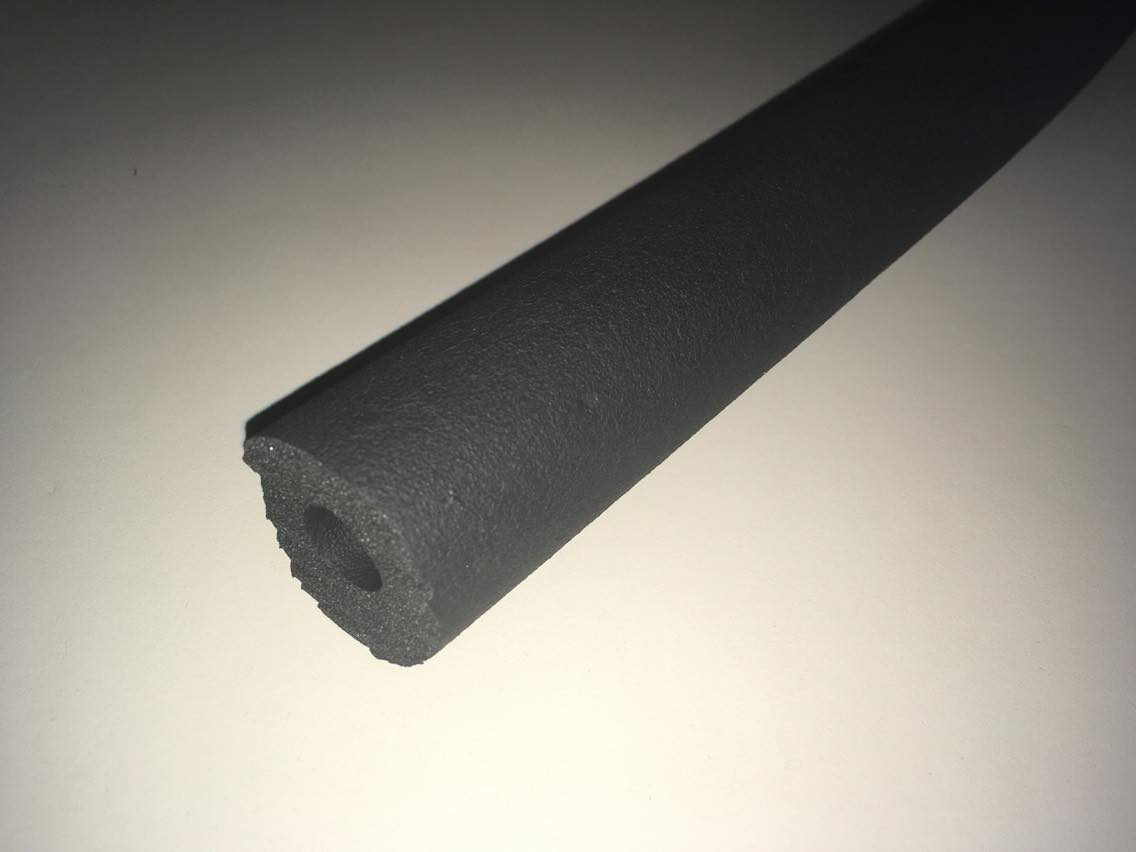
\includegraphics{./pictures/pipe.jpg}}
	\end{center}
	\caption{Isolating pipe}
	\label{rys:pipe}
\end{figure}

At the beginning proposed solution of exploiting needles in order to measure humidity has to be explored thoroughly. Set of measurements were collected in time from complete dry isolation to fully wet and full of water. Experiments were performed for 30 minutes using \verb|Hewlett| \verb|Packard| \verb|4263B| \verb|LCR Meter| (\figurename{} \ref{rys:hewlett}), which was connected to the PC via \verb|GPIB-USB-HS| control device and \verb|MATLAB| where communication with \verb|LCR Meter| was implemented.

\begin{figure}[H]
	\begin{center}
		\scalebox{.25}{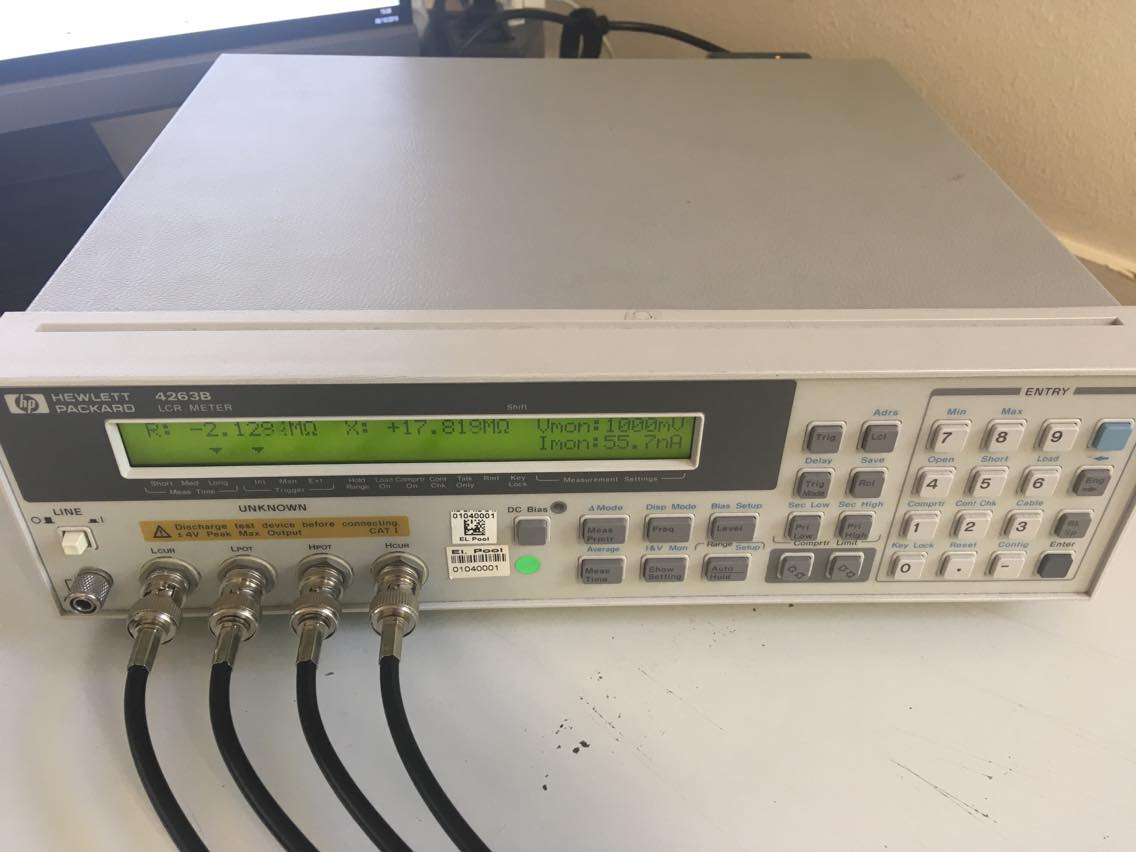
\includegraphics{./pictures/hewlett.jpg}}
	\end{center}
	\caption{Hewlett Packard 4263B LCR Meter}
	\label{rys:hewlett}
\end{figure}

The \verb|LCR| \verb|meter| allows to perform measurements of different quantities like capacitance or impedance. For the project purpose the device was configured to measure resistance. Both the device and the measurement configuration were performed in \verb|MATLAB| using \verb|Basic| language and commands.

A pair of needles were mounted on a calipers as shown on \figurename{} \ref{rys:needles} in order to exactly set and monitor the needles distance and verify that both are in the same depth. All the experiments were performed with isolation placed on the floor horizontally as well as the calipers. 

\begin{figure}[H]
	\begin{center}
		\scalebox{.25}{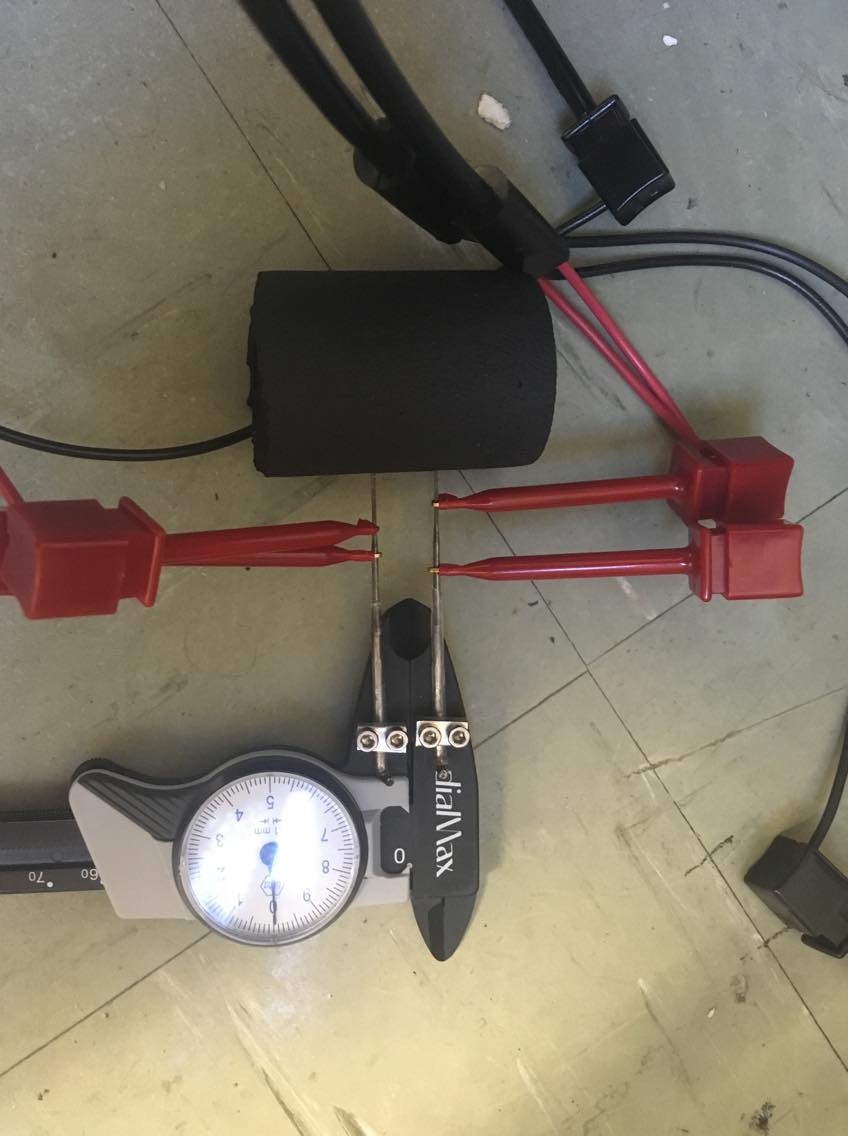
\includegraphics[angle=90,origin=c]{./pictures/needles.jpg}}
	\end{center}
	\caption{Needles mounted on the calipers with connected LCR Meter}
	\label{rys:needles}
\end{figure}

\section{Experiments}
A couple of experiments were performed with different needles configuration, that is a place of sticking into isolation and different amount of water. 
Needles were placed in three ways. First they pierced fully isolation in the middle, consequently they were stuck to the top and bottom edge also horizontally, what means that the needles did not crossed inner hole of the isolation. The last experiment was performed with the needles stuck in the middle, however only to the depth of 1cm -- before they reached an inner hole. 

\begin{figure}[H]
	\begin{center}
		\scalebox{.7}{% This file was created by matlab2tikz.
%
%The latest updates can be retrieved from
%  http://www.mathworks.com/matlabcentral/fileexchange/22022-matlab2tikz-matlab2tikz
%where you can also make suggestions and rate matlab2tikz.
%
\definecolor{mycolor1}{rgb}{0.00000,0.44700,0.74100}%
%
\begin{tikzpicture}

\begin{axis}[%
width=4.521in,
height=3.566in,
at={(0.758in,0.481in)},
scale only axis,
xmin=0,
xmax=30,
xlabel style={font=\color{white!15!black}},
xlabel={t},
ymin=-10000,
ymax=230626000,
ylabel style={font=\color{white!15!black}},
ylabel={R},
axis background/.style={fill=white},
xmajorgrids,
ymajorgrids,
legend style={legend cell align=left, align=left, draw=white!15!black}
]
\addplot [color=mycolor1]
  table[row sep=crcr]{%
0	85135700\\
0.01667	104307000\\
0.03334	99810400\\
0.05001	86722800\\
0.06668	101016000\\
0.08335	83570500\\
0.10002	122970000\\
0.11669	109422000\\
0.13336	97676100\\
0.15003	100366000\\
0.1667	103080000\\
0.18337	118850000\\
0.20004	78201900\\
0.21671	119926000\\
0.23338	87707900\\
0.25005	89795800\\
0.26672	102566000\\
0.28339	93943500\\
0.30006	105891000\\
0.31673	112400000\\
0.3334	98382400\\
0.35007	114188000\\
0.36674	98119600\\
0.38341	89768400\\
0.40008	101453000\\
0.41675	115252000\\
0.43342	117577000\\
0.45009	125183000\\
0.46676	128292000\\
0.48343	127022000\\
0.5001	138459000\\
0.51677	120607000\\
0.53344	136423000\\
0.55011	119849000\\
0.56678	131306000\\
0.58345	116699000\\
0.60012	101256000\\
0.61679	145725000\\
0.63346	167937000\\
0.65013	176639000\\
0.6668	179339000\\
0.68347	148686000\\
0.70014	176535000\\
0.71681	173546000\\
0.73348	167267000\\
0.75015	176257000\\
0.76682	156604000\\
0.78349	207126000\\
0.80016	185202000\\
0.81683	183992000\\
0.8335	195781000\\
0.85017	194707000\\
0.86684	162772000\\
0.88351	184969000\\
0.90018	181625000\\
0.91685	152426000\\
0.93352	116416000\\
0.95019	118296000\\
0.96686	114586000\\
0.98353	137691000\\
1.0002	81371500\\
1.01687	106485000\\
1.03354	90836700\\
1.05021	99746200\\
1.06688	111222000\\
1.08355	115719000\\
1.10022	89918600\\
1.11689	111136000\\
1.13356	105068000\\
1.15023	97698200\\
1.1669	87995700\\
1.18357	119660000\\
1.20024	105913000\\
1.21691	104971000\\
1.23358	121543000\\
1.25025	105704000\\
1.26692	128863000\\
1.28359	103056000\\
1.30026	125302000\\
1.31693	125137000\\
1.3336	120300000\\
1.35027	116906000\\
1.36694	128346000\\
1.38361	98011600\\
1.40028	125105000\\
1.41695	106380000\\
1.43362	103783000\\
1.45029	102021000\\
1.46696	79959500\\
1.48363	77993200\\
1.5003	82354100\\
1.51697	84112600\\
1.53364	104307000\\
1.55031	111456000\\
1.56698	101604000\\
1.58365	99773200\\
1.60032	113584000\\
1.61699	150180000\\
1.63366	171272000\\
1.65033	179897000\\
1.667	189469000\\
1.68367	202043000\\
1.70034	208154000\\
1.71701	209808000\\
1.73368	172048000\\
1.75035	173684000\\
1.76702	158608000\\
1.78369	104024000\\
1.80036	110000000\\
1.81703	93330100\\
1.8337	100760000\\
1.85037	126506000\\
1.86704	111685000\\
1.88371	130877000\\
1.90038	143213000\\
1.91705	180749000\\
1.93372	191488000\\
1.95039	213452000\\
1.96706	185600000\\
1.98373	165925000\\
2.0004	145394000\\
2.01707	132541000\\
2.03374	109995000\\
2.05041	77515800\\
2.06708	103125000\\
2.08375	92461900\\
2.10042	139286000\\
2.11709	146120000\\
2.13376	183182000\\
2.15043	179224000\\
2.1671	195003000\\
2.18377	192092000\\
2.20044	208061000\\
2.21711	151813000\\
2.23378	167692000\\
2.25045	111630000\\
2.26712	92900400\\
2.28379	125798000\\
2.30046	94794600\\
2.31713	122392000\\
2.3338	129534000\\
2.35047	189246000\\
2.36714	190605000\\
2.38381	203351000\\
2.40048	222102000\\
2.41715	161122000\\
2.43382	166436000\\
2.45049	149723000\\
2.46716	134712000\\
2.48383	109773000\\
2.5005	93811600\\
2.51717	89069600\\
2.53384	106366000\\
2.55051	134706000\\
2.56718	152103000\\
2.58385	161300000\\
2.60052	195157000\\
2.61719	190517000\\
2.63386	195709000\\
2.65053	212511000\\
2.6672	219786000\\
2.68387	179639000\\
2.70054	228516000\\
2.71721	150174000\\
2.73388	153765000\\
2.75055	161288000\\
2.76722	129091000\\
2.78389	102196000\\
2.80056	85082700\\
2.81723	88823400\\
2.8339	107417000\\
2.85057	92823900\\
2.86724	119632000\\
2.88391	106394000\\
2.90058	156696000\\
2.91725	124773000\\
2.93392	135893000\\
2.95059	175694000\\
2.96726	164825000\\
2.98393	169443000\\
3.0006	185847000\\
3.01727	209552000\\
3.03394	208686000\\
3.05061	207248000\\
3.06728	198879000\\
3.08395	158892000\\
3.10062	165685000\\
3.11729	150875000\\
3.13396	136812000\\
3.15063	101819000\\
3.1673	97366300\\
3.18397	113527000\\
3.20064	94101600\\
3.21731	117273000\\
3.23398	116615000\\
3.25065	115647000\\
3.26732	141775000\\
3.28399	131856000\\
3.30066	164519000\\
3.31733	155588000\\
3.334	175571000\\
3.35067	199210000\\
3.36734	208716000\\
3.38401	206096000\\
3.40068	197268000\\
3.41735	165123000\\
3.43402	192227000\\
3.45069	178133000\\
3.46736	136148000\\
3.48403	111003000\\
3.5007	128201000\\
3.51737	104270000\\
3.53404	112259000\\
3.55071	82774100\\
3.56738	100846000\\
3.58405	96578800\\
3.60072	81642600\\
3.61739	93017000\\
3.63406	102237000\\
3.65073	102696000\\
3.6674	93715900\\
3.68407	95253700\\
3.70074	112497000\\
3.71741	95505800\\
3.73408	91190500\\
3.75075	114098000\\
3.76742	119388000\\
3.78409	104026000\\
3.80076	82784100\\
3.81743	107091000\\
3.8341	112353000\\
3.85077	125329000\\
3.86744	103353000\\
3.88411	126002000\\
3.90078	152083000\\
3.91745	143245000\\
3.93412	130590000\\
3.95079	145925000\\
3.96746	137573000\\
3.98413	156481000\\
4.0008	144402000\\
4.01747	121808000\\
4.03414	141344000\\
4.05081	107661000\\
4.06748	110739000\\
4.08415	107232000\\
4.10082	105032000\\
4.11749	89465900\\
4.13416	99820100\\
4.15083	127207000\\
4.1675	108643000\\
4.18417	111724000\\
4.20084	134608000\\
4.21751	138224000\\
4.23418	148628000\\
4.25085	171302000\\
4.26752	183481000\\
4.28419	201055000\\
4.30086	211778000\\
4.31753	205093000\\
4.3342	196130000\\
4.35087	188580000\\
4.36754	222530000\\
4.38421	182320000\\
4.40088	197648000\\
4.41755	196676000\\
4.43422	209313000\\
4.45089	181798000\\
4.46756	199046000\\
4.48423	203810000\\
4.5009	195081000\\
4.51757	174065000\\
4.53424	190023000\\
4.55091	189911000\\
4.56758	187976000\\
4.58425	176627000\\
4.60092	130946000\\
4.61759	153470000\\
4.63426	144282000\\
4.65093	127314000\\
4.6676	138426000\\
4.68427	166144000\\
4.70094	145393000\\
4.71761	140508000\\
4.73428	126951000\\
4.75095	117687000\\
4.76762	142346000\\
4.78429	131513000\\
4.80096	144302000\\
4.81763	140893000\\
4.8343	169576000\\
4.85097	183679000\\
4.86764	149388000\\
4.88431	152218000\\
4.90098	163784000\\
4.91765	178053000\\
4.93432	175630000\\
4.95099	166812000\\
4.96766	194686000\\
4.98433	193740000\\
5.001	218269000\\
5.01767	215899000\\
5.03434	195400000\\
5.05101	196288000\\
5.06768	207470000\\
5.08435	183832000\\
5.10102	212940000\\
5.11769	153297000\\
5.13436	159961000\\
5.15103	165275000\\
5.1677	148722000\\
5.18437	142360000\\
5.20104	115014000\\
5.21771	120961000\\
5.23438	126578000\\
5.25105	118414000\\
5.26772	94085300\\
5.28439	129178000\\
5.30106	92346300\\
5.31773	98266800\\
5.3344	82753000\\
5.35107	113020000\\
5.36774	78762700\\
5.38441	108718000\\
5.40108	90813000\\
5.41775	89210600\\
5.43442	105668000\\
5.45109	86215800\\
5.46776	86079300\\
5.48443	98172100\\
5.5011	112893000\\
5.51777	80656600\\
5.53444	97403300\\
5.55111	98351600\\
5.56778	78553400\\
5.58445	89225200\\
5.60112	113249000\\
5.61779	105978000\\
5.63446	104827000\\
5.65113	104201000\\
5.6678	107442000\\
5.68447	144571000\\
5.70114	149340000\\
5.71781	129286000\\
5.73448	119952000\\
5.75115	153729000\\
5.76782	170753000\\
5.78449	186770000\\
5.80116	184325000\\
5.81783	194543000\\
5.8345	212072000\\
5.85117	203922000\\
5.86784	189912000\\
5.88451	201507000\\
5.90118	197675000\\
5.91785	157471000\\
5.93452	141405000\\
5.95119	145069000\\
5.96786	96774000\\
5.98453	80035200\\
6.0012	119465000\\
6.01787	92352800\\
6.03454	92664500\\
6.05121	80390300\\
6.06788	80003500\\
6.08455	111180000\\
6.10122	98223000\\
6.11789	84415000\\
6.13456	112120000\\
6.15123	87234300\\
6.1679	117972000\\
6.18457	64942100\\
6.20124	105005000\\
6.21791	98152000\\
6.23458	100233000\\
6.25125	107474000\\
6.26792	97760900\\
6.28459	90308200\\
6.30126	103164000\\
6.31793	110628000\\
6.3346	117862000\\
6.35127	134095000\\
6.36794	120214000\\
6.38461	117715000\\
6.40128	103357000\\
6.41795	95217500\\
6.43462	131864000\\
6.45129	114987000\\
6.46796	128018000\\
6.48463	97567100\\
6.5013	121577000\\
6.51797	129414000\\
6.53464	139236000\\
6.55131	156653000\\
6.56798	130578000\\
6.58465	131985000\\
6.60132	162346000\\
6.61799	153878000\\
6.63466	152300000\\
6.65133	180764000\\
6.668	176031000\\
6.68467	190465000\\
6.70134	204961000\\
6.71801	181115000\\
6.73468	192139000\\
6.75135	186655000\\
6.76802	217218000\\
6.78469	190115000\\
6.80136	222834000\\
6.81803	190196000\\
6.8347	179510000\\
6.85137	183455000\\
6.86804	199250000\\
6.88471	195693000\\
6.90138	189718000\\
6.91805	159727000\\
6.93472	150519000\\
6.95139	137239000\\
6.96806	100822000\\
6.98473	112903000\\
7.0014	88680400\\
7.01807	96658300\\
7.03474	113892000\\
7.05141	86479500\\
7.06808	67346500\\
7.08475	76502200\\
7.10142	96080800\\
7.11809	110041000\\
7.13476	128098000\\
7.15143	120064000\\
7.1681	139147000\\
7.18477	119726000\\
7.20144	132447000\\
7.21811	122814000\\
7.23478	143793000\\
7.25145	147086000\\
7.26812	129023000\\
7.28479	130584000\\
7.30146	156300000\\
7.31813	152513000\\
7.3348	151925000\\
7.35147	143784000\\
7.36814	150666000\\
7.38481	168826000\\
7.40148	166644000\\
7.41815	142735000\\
7.43482	158454000\\
7.45149	167568000\\
7.46816	152073000\\
7.48483	151612000\\
7.5015	120724000\\
7.51817	120344000\\
7.53484	100466000\\
7.55151	107097000\\
7.56818	122240000\\
7.58485	120282000\\
7.60152	108189000\\
7.61819	80823900\\
7.63486	120518000\\
7.65153	131446000\\
7.6682	134338000\\
7.68487	158883000\\
7.70154	167254000\\
7.71821	152649000\\
7.73488	179302000\\
7.75155	201605000\\
7.76822	209354000\\
7.78489	190420000\\
7.80156	194617000\\
7.81823	198696000\\
7.8349	146872000\\
7.85157	131849000\\
7.86824	94225200\\
7.88491	112658000\\
7.90158	100023000\\
7.91825	97539000\\
7.93492	74483800\\
7.95159	102127000\\
7.96826	87868100\\
7.98493	118434000\\
8.0016	123480000\\
8.01827	142657000\\
8.03494	131524000\\
8.05161	181060000\\
8.06828	174337000\\
8.08495	181522000\\
8.10162	188142000\\
8.11829	188105000\\
8.13496	207913000\\
8.15163	208808000\\
8.1683	187729000\\
8.18497	200753000\\
8.20164	183379000\\
8.21831	190841000\\
8.23498	137691000\\
8.25165	129760000\\
8.26832	118330000\\
8.28499	127845000\\
8.30166	96082000\\
8.31833	112578000\\
8.335	87372100\\
8.35167	105745000\\
8.36834	110255000\\
8.38501	93819900\\
8.40168	109978000\\
8.41835	88630400\\
8.43502	101654000\\
8.45169	108408000\\
8.46836	86301700\\
8.48503	127505000\\
8.5017	135194000\\
8.51837	154371000\\
8.53504	155344000\\
8.55171	177717000\\
8.56838	173507000\\
8.58505	186824000\\
8.60172	200906000\\
8.61839	215488000\\
8.63506	198463000\\
8.65173	186102000\\
8.6684	215416000\\
8.68507	160940000\\
8.70174	163883000\\
8.71841	140870000\\
8.73508	138905000\\
8.75175	132117000\\
8.76842	100605000\\
8.78509	102638000\\
8.80176	86355500\\
8.81843	86711800\\
8.8351	104641000\\
8.85177	76180200\\
8.86844	81961000\\
8.88511	90582500\\
8.90178	119477000\\
8.91845	118051000\\
8.93512	95652500\\
8.95179	104848000\\
8.96846	134033000\\
8.98513	133167000\\
9.0018	153191000\\
9.01847	148179000\\
9.03514	198677000\\
9.05181	167490000\\
9.06848	198107000\\
9.08515	190625000\\
9.10182	214430000\\
9.11849	179807000\\
9.13516	190168000\\
9.15183	189237000\\
9.1685	175124000\\
9.18517	186031000\\
9.20184	162906000\\
9.21851	178467000\\
9.23518	147493000\\
9.25185	121643000\\
9.26852	84850200\\
9.28519	101674000\\
9.30186	117309000\\
9.31853	113132000\\
9.3352	95438400\\
9.35187	99055700\\
9.36854	87207800\\
9.38521	105108000\\
9.40188	114908000\\
9.41855	109327000\\
9.43522	124095000\\
9.45189	143533000\\
9.46856	148534000\\
9.48523	167227000\\
9.5019	162003000\\
9.51857	210481000\\
9.53524	207939000\\
9.55191	186487000\\
9.56858	174837000\\
9.58525	167386000\\
9.60192	198624000\\
9.61859	152938000\\
9.63526	168185000\\
9.65193	144052000\\
9.6686	146165000\\
9.68527	124157000\\
9.70194	121374000\\
9.71861	123472000\\
9.73528	91017600\\
9.75195	113784000\\
9.76862	98506400\\
9.78529	105001000\\
9.80196	109108000\\
9.81863	107194000\\
9.8353	117517000\\
9.85197	128424000\\
9.86864	130520000\\
9.88531	180744000\\
9.90198	150982000\\
9.91865	175872000\\
9.93532	184955000\\
9.95199	208648000\\
9.96866	221619000\\
9.98533	189679000\\
10.002	209407000\\
10.01867	198281000\\
10.03534	176315000\\
10.05201	176755000\\
10.06868	174580000\\
10.08535	176531000\\
10.10202	178299000\\
10.11869	177566000\\
10.13536	171051000\\
10.15203	162619000\\
10.1687	129589000\\
10.18537	172805000\\
10.20204	147039000\\
10.21871	135714000\\
10.23538	116511000\\
10.25205	116046000\\
10.26872	90124500\\
10.28539	89321500\\
10.30206	110659000\\
10.31873	93185400\\
10.3354	100792000\\
10.35207	109883000\\
10.36874	95298200\\
10.38541	103007000\\
10.40208	108439000\\
10.41875	101395000\\
10.43542	144919000\\
10.45209	103877000\\
10.46876	133738000\\
10.48543	113401000\\
10.5021	165778000\\
10.51877	182543000\\
10.53544	170451000\\
10.55211	166147000\\
10.56878	173871000\\
10.58545	163415000\\
10.60212	172881000\\
10.61879	180449000\\
10.63546	176671000\\
10.65213	191961000\\
10.6688	198370000\\
10.68547	188278000\\
10.70214	199004000\\
10.71881	173611000\\
10.73548	200793000\\
10.75215	197055000\\
10.76882	172668000\\
10.78549	181919000\\
10.80216	133878000\\
10.81883	123769000\\
10.8355	106209000\\
10.85217	88424200\\
10.86884	94392300\\
10.88551	82812100\\
10.90218	86681400\\
10.91885	110927000\\
10.93552	100395000\\
10.95219	137903000\\
10.96886	104411000\\
10.98553	119876000\\
11.0022	133186000\\
11.01887	140260000\\
11.03554	148669000\\
11.05221	141944000\\
11.06888	161753000\\
11.08555	163410000\\
11.10222	201952000\\
11.11889	183020000\\
11.13556	190765000\\
11.15223	213062000\\
11.1689	210705000\\
11.18557	177804000\\
11.20224	164539000\\
11.21891	148282000\\
11.23558	133467000\\
11.25225	93893000\\
11.26892	114092000\\
11.28559	106234000\\
11.30226	90092100\\
11.31893	108741000\\
11.3356	107633000\\
11.35227	123687000\\
11.36894	127917000\\
11.38561	156036000\\
11.40228	166766000\\
11.41895	191235000\\
11.43562	180178000\\
11.45229	189169000\\
11.46896	180604000\\
11.48563	187323000\\
11.5023	209878000\\
11.51897	182977000\\
11.53564	172529000\\
11.55231	144262000\\
11.56898	110906000\\
11.58565	122347000\\
11.60232	105668000\\
11.61899	97603200\\
11.63566	99977200\\
11.65233	117186000\\
11.669	118048000\\
11.68567	115759000\\
11.70234	156935000\\
11.71901	156524000\\
11.73568	192278000\\
11.75235	189121000\\
11.76902	200146000\\
11.78569	184981000\\
11.80236	188935000\\
11.81903	139383000\\
11.8357	129570000\\
11.85237	113902000\\
11.86904	99260800\\
11.88571	84410400\\
11.90238	117820000\\
11.91905	123570000\\
11.93572	136280000\\
11.95239	151869000\\
11.96906	163847000\\
11.98573	196747000\\
12.0024	197694000\\
12.01907	209005000\\
12.03574	163380000\\
12.05241	170814000\\
12.06908	155154000\\
12.08575	122702000\\
12.10242	101116000\\
12.11909	95939500\\
12.13576	86007000\\
12.15243	120665000\\
12.1691	138210000\\
12.18577	155359000\\
12.20244	176831000\\
12.21911	210025000\\
12.23578	193271000\\
12.25245	177030000\\
12.26912	177529000\\
12.28579	184663000\\
12.30246	184123000\\
12.31913	127520000\\
12.3358	108326000\\
12.35247	108911000\\
12.36914	107210000\\
12.38581	103127000\\
12.40248	106553000\\
12.41915	80578900\\
12.43582	93115300\\
12.45249	122806000\\
12.46916	128937000\\
12.48583	125743000\\
12.5025	124488000\\
12.51917	165753000\\
12.53584	180060000\\
12.55251	154827000\\
12.56918	167806000\\
12.58585	178021000\\
12.60252	188335000\\
12.61919	196759000\\
12.63586	167523000\\
12.65253	202625000\\
12.6692	184174000\\
12.68587	214240000\\
12.70254	202571000\\
12.71921	203985000\\
12.73588	197976000\\
12.75255	194771000\\
12.76922	204772000\\
12.78589	182520000\\
12.80256	182130000\\
12.81923	186577000\\
12.8359	172302000\\
12.85257	119006000\\
12.86924	149039000\\
12.88591	110821000\\
12.90258	94443800\\
12.91925	100839000\\
12.93592	104813000\\
12.95259	111226000\\
12.96926	97045300\\
12.98593	84140800\\
13.0026	84677500\\
13.01927	112654000\\
13.03594	129416000\\
13.05261	109561000\\
13.06928	119592000\\
13.08595	122892000\\
13.10262	116073000\\
13.11929	148710000\\
13.13596	174982000\\
13.15263	157658000\\
13.1693	139507000\\
13.18597	156274000\\
13.20264	195173000\\
13.21931	183309000\\
13.23598	179135000\\
13.25265	209815000\\
13.26932	183550000\\
13.28599	198048000\\
13.30266	218519000\\
13.31933	203046000\\
13.336	202625000\\
13.35267	159191000\\
13.36934	152653000\\
13.38601	144528000\\
13.40268	130405000\\
13.41935	129855000\\
13.43602	107763000\\
13.45269	84247300\\
13.46936	98358000\\
13.48603	95701200\\
13.5027	72496000\\
13.51937	83395900\\
13.53604	89479900\\
13.55271	98152000\\
13.56938	87767500\\
13.58605	79197200\\
13.60272	91519600\\
13.61939	103921000\\
13.63606	110686000\\
13.65273	134747000\\
13.6694	100776000\\
13.68607	130041000\\
13.70274	110044000\\
13.71941	134947000\\
13.73608	150456000\\
13.75275	182306000\\
13.76942	173566000\\
13.78609	189211000\\
13.80276	198870000\\
13.81943	204701000\\
13.8361	197233000\\
13.85277	198833000\\
13.86944	192098000\\
13.88611	193650000\\
13.90278	161486000\\
13.91945	159697000\\
13.93612	170527000\\
13.95279	151780000\\
13.96946	147414000\\
13.98613	145806000\\
14.0028	133232000\\
14.01947	153721000\\
14.03614	137826000\\
14.05281	155764000\\
14.06948	145623000\\
14.08615	139377000\\
14.10282	126566000\\
14.11949	100780000\\
14.13616	129074000\\
14.15283	119298000\\
14.1695	99219600\\
14.18617	101498000\\
14.20284	103526000\\
14.21951	105379000\\
14.23618	75764900\\
14.25285	112414000\\
14.26952	102667000\\
14.28619	114679000\\
14.30286	105904000\\
14.31953	91959700\\
14.3362	95942000\\
14.35287	112708000\\
14.36954	117128000\\
14.38621	100572000\\
14.40288	109565000\\
14.41955	119289000\\
14.43622	120922000\\
14.45289	143729000\\
14.46956	130936000\\
14.48623	152932000\\
14.5029	159853000\\
14.51957	184023000\\
14.53624	185677000\\
14.55291	197525000\\
14.56958	170391000\\
14.58625	202006000\\
14.60292	216899000\\
14.61959	195141000\\
14.63626	213522000\\
14.65293	197512000\\
14.6696	190683000\\
14.68627	191124000\\
14.70294	201018000\\
14.71961	190243000\\
14.73628	174034000\\
14.75295	173804000\\
14.76962	199189000\\
14.78629	170692000\\
14.80296	158082000\\
14.81963	201730000\\
14.8363	139118000\\
14.85297	140111000\\
14.86964	156400000\\
14.88631	145642000\\
14.90298	142043000\\
14.91965	99626100\\
14.93632	131647000\\
14.95299	100079000\\
14.96966	79778600\\
14.98633	102468000\\
15.003	96583700\\
15.01967	94221200\\
15.03634	94343900\\
15.05301	122731000\\
15.06968	116125000\\
15.08635	112427000\\
15.10302	116193000\\
15.11969	144853000\\
15.13636	149266000\\
15.15303	203167000\\
15.1697	180849000\\
15.18637	185654000\\
15.20304	218156000\\
15.21971	182783000\\
15.23638	193971000\\
15.25305	183594000\\
15.26972	145831000\\
15.28639	162854000\\
15.30306	145567000\\
15.31973	125059000\\
15.3364	121984000\\
15.35307	107330000\\
15.36974	101578000\\
15.38641	90033800\\
15.40308	105311000\\
15.41975	109736000\\
15.43642	105846000\\
15.45309	103018000\\
15.46976	112547000\\
15.48643	154203000\\
15.5031	139151000\\
15.51977	169328000\\
15.53644	158250000\\
15.55311	163586000\\
15.56978	179366000\\
15.58645	200980000\\
15.60312	198339000\\
15.61979	192935000\\
15.63646	217925000\\
15.65313	211503000\\
15.6698	190590000\\
15.68647	161027000\\
15.70314	204185000\\
15.71981	198538000\\
15.73648	177835000\\
15.75315	187211000\\
15.76982	191075000\\
15.78649	173090000\\
15.80316	174115000\\
15.81983	153130000\\
15.8365	176061000\\
15.85317	156972000\\
15.86984	182889000\\
15.88651	166689000\\
15.90318	157329000\\
15.91985	146468000\\
15.93652	135447000\\
15.95319	142220000\\
15.96986	107778000\\
15.98653	109240000\\
16.0032	105785000\\
16.01987	104236000\\
16.03654	109890000\\
16.05321	116824000\\
16.06988	98701200\\
16.08655	92511700\\
16.10322	106738000\\
16.11989	129284000\\
16.13656	124629000\\
16.15323	124169000\\
16.1699	114897000\\
16.18657	123084000\\
16.20324	121195000\\
16.21991	135493000\\
16.23658	142132000\\
16.25325	128881000\\
16.26992	144893000\\
16.28659	182364000\\
16.30326	163946000\\
16.31993	194146000\\
16.3366	208186000\\
16.35327	192347000\\
16.36994	213199000\\
16.38661	221421000\\
16.40328	194396000\\
16.41995	186979000\\
16.43662	186744000\\
16.45329	182086000\\
16.46996	197036000\\
16.48663	209381000\\
16.5033	190114000\\
16.51997	182059000\\
16.53664	185686000\\
16.55331	175182000\\
16.56998	154774000\\
16.58665	163531000\\
16.60332	225212000\\
16.61999	208835000\\
16.63666	197387000\\
16.65333	192432000\\
16.67	199400000\\
16.68667	230626000\\
16.70334	203190000\\
16.72001	172909000\\
16.73668	197329000\\
16.75335	184642000\\
16.77002	179494000\\
16.78669	215873000\\
16.80336	190695000\\
16.82003	170749000\\
16.8367	150188000\\
16.85337	171633000\\
16.87004	138381000\\
16.88671	151019000\\
16.90338	162563000\\
16.92005	130303000\\
16.93672	116579000\\
16.95339	107782000\\
16.97006	120520000\\
16.98673	122356000\\
17.0034	107896000\\
17.02007	89085600\\
17.03674	128146000\\
17.05341	102857000\\
17.07008	107939000\\
17.08675	102493000\\
17.10342	100181000\\
17.12009	88451700\\
17.13676	113199000\\
17.15343	111573000\\
17.1701	110049000\\
17.18677	100322000\\
17.20344	113297000\\
17.22011	131386000\\
17.23678	100660000\\
17.25345	135322000\\
17.27012	94835700\\
17.28679	121586000\\
17.30346	108679000\\
17.32013	103506000\\
17.3368	118336000\\
17.35347	88096900\\
17.37014	100481000\\
17.38681	70620500\\
17.40348	88568400\\
17.42015	100560000\\
17.43682	96061300\\
17.45349	94409200\\
17.47016	115737000\\
17.48683	111948000\\
17.5035	131540000\\
17.52017	128005000\\
17.53684	133138000\\
17.55351	123471000\\
17.57018	141680000\\
17.58685	141523000\\
17.60352	167090000\\
17.62019	144585000\\
17.63686	149473000\\
17.65353	164968000\\
17.6702	124872000\\
17.68687	139324000\\
17.70354	155767000\\
17.72021	150543000\\
17.73688	148918000\\
17.75355	144159000\\
17.77022	169109000\\
17.78689	177918000\\
17.80356	168222000\\
17.82023	147540000\\
17.8369	137885000\\
17.85357	158861000\\
17.87024	152483000\\
17.88691	151024000\\
17.90358	155805000\\
17.92025	159888000\\
17.93692	158199000\\
17.95359	144231000\\
17.97026	123851000\\
17.98693	112104000\\
18.0036	106049000\\
18.02027	117266000\\
18.03694	117249000\\
18.05361	101683000\\
18.07028	84405400\\
18.08695	107567000\\
18.10362	91922500\\
18.12029	76500900\\
18.13696	115398000\\
18.15363	92659400\\
18.1703	100435000\\
18.18697	105853000\\
18.20364	122662000\\
18.22031	109630000\\
18.23698	134196000\\
18.25365	120977000\\
18.27032	110528000\\
18.28699	120760000\\
18.30366	103348000\\
18.32033	133146000\\
18.337	126991000\\
18.35367	114208000\\
18.37034	99735500\\
18.38701	136440000\\
18.40368	119461000\\
18.42035	117944000\\
18.43702	138034000\\
18.45369	138084000\\
18.47036	108572000\\
18.48703	118810000\\
18.5037	112602000\\
18.52037	119917000\\
18.53704	86627000\\
18.55371	107318000\\
18.57038	112445000\\
18.58705	107537000\\
18.60372	113522000\\
18.62039	122374000\\
18.63706	106084000\\
18.65373	103740000\\
18.6704	102418000\\
18.68707	97639800\\
18.70374	106362000\\
18.72041	115353000\\
18.73708	113138000\\
18.75375	93956900\\
18.77042	85782800\\
18.78709	117190000\\
18.80376	103370000\\
18.82043	90987500\\
18.8371	83727900\\
18.85377	83280700\\
18.87044	100231000\\
18.88711	109086000\\
18.90378	89929500\\
18.92045	92125800\\
18.93712	105777000\\
18.95379	101768000\\
18.97046	107182000\\
18.98713	115685000\\
19.0038	118986000\\
19.02047	157623000\\
19.03714	129024000\\
19.05381	161558000\\
19.07048	149269000\\
19.08715	165174000\\
19.10382	167364000\\
19.12049	187483000\\
19.13716	179807000\\
19.15383	181976000\\
19.1705	209440000\\
19.18717	223181000\\
19.20384	185169000\\
19.22051	208802000\\
19.23718	197785000\\
19.25385	174781000\\
19.27052	154874000\\
19.28719	173519000\\
19.30386	147530000\\
19.32053	160215000\\
19.3372	164047000\\
19.35387	151066000\\
19.37054	132512000\\
19.38721	117586000\\
19.40388	123456000\\
19.42055	108501000\\
19.43722	118473000\\
19.45389	125862000\\
19.47056	108544000\\
19.48723	105821000\\
19.5039	114671000\\
19.52057	97718200\\
19.53724	106059000\\
19.55391	104075000\\
19.57058	83873900\\
19.58725	94114600\\
19.60392	94641900\\
19.62059	90229100\\
19.63726	88202500\\
19.65393	106216000\\
19.6706	98263200\\
19.68727	108431000\\
19.70394	115048000\\
19.72061	139553000\\
19.73728	138364000\\
19.75395	147733000\\
19.77062	141830000\\
19.78729	174847000\\
19.80396	170595000\\
19.82063	193885000\\
19.8373	175332000\\
19.85397	184734000\\
19.87064	197585000\\
19.88731	184392000\\
19.90398	179553000\\
19.92065	165494000\\
19.93732	167163000\\
19.95399	187171000\\
19.97066	163627000\\
19.98733	165034000\\
20.004	147934000\\
20.02067	138972000\\
20.03734	128153000\\
20.05401	106270000\\
20.07068	123326000\\
20.08735	121911000\\
20.10402	150213000\\
20.12069	130037000\\
20.13736	128045000\\
20.15403	129764000\\
20.1707	107002000\\
20.18737	102357000\\
20.20404	119819000\\
20.22071	104923000\\
20.23738	125825000\\
20.25405	106892000\\
20.27072	132685000\\
20.28739	127393000\\
20.30406	123682000\\
20.32073	114596000\\
20.3374	155014000\\
20.35407	119362000\\
20.37074	156223000\\
20.38741	175551000\\
20.40408	159275000\\
20.42075	140497000\\
20.43742	157553000\\
20.45409	195789000\\
20.47076	191682000\\
20.48743	183051000\\
20.5041	226340000\\
20.52077	189253000\\
20.53744	205477000\\
20.55411	200048000\\
20.57078	191376000\\
20.58745	191498000\\
20.60412	176233000\\
20.62079	186344000\\
20.63746	158377000\\
20.65413	162162000\\
20.6708	149495000\\
20.68747	147162000\\
20.70414	126623000\\
20.72081	137632000\\
20.73748	119470000\\
20.75415	110891000\\
20.77082	99299300\\
20.78749	101608000\\
20.80416	89889900\\
20.82083	91857200\\
20.8375	91866800\\
20.85417	80156200\\
20.87084	96988100\\
20.88751	118638000\\
20.90418	104033000\\
20.92085	132877000\\
20.93752	119754000\\
20.95419	150188000\\
20.97086	188980000\\
20.98753	199420000\\
21.0042	194955000\\
21.02087	197527000\\
21.03754	209598000\\
21.05421	218563000\\
21.07088	214690000\\
21.08755	206820000\\
21.10422	184641000\\
21.12089	202385000\\
21.13756	185383000\\
21.15423	186664000\\
21.1709	186906000\\
21.18757	190021000\\
21.20424	182243000\\
21.22091	196076000\\
21.23758	162296000\\
21.25425	148254000\\
21.27092	170938000\\
21.28759	162034000\\
21.30426	148503000\\
21.32093	181415000\\
21.3376	188092000\\
21.35427	176448000\\
21.37094	157874000\\
21.38761	162916000\\
21.40428	157491000\\
21.42095	160262000\\
21.43762	170791000\\
21.45429	167220000\\
21.47096	151114000\\
21.48763	148877000\\
21.5043	143562000\\
21.52097	117641000\\
21.53764	137337000\\
21.55431	128901000\\
21.57098	129571000\\
21.58765	124813000\\
21.60432	91213200\\
21.62099	105500000\\
21.63766	117143000\\
21.65433	89177300\\
21.671	97808000\\
21.68767	102175000\\
21.70434	97073600\\
21.72101	99198500\\
21.73768	123278000\\
21.75435	118229000\\
21.77102	81410900\\
21.78769	108981000\\
21.80436	100526000\\
21.82103	112551000\\
21.8377	114201000\\
21.85437	106030000\\
21.87104	124185000\\
21.88771	138345000\\
21.90438	126328000\\
21.92105	133028000\\
21.93772	128490000\\
21.95439	159378000\\
21.97106	137603000\\
21.98773	132704000\\
22.0044	163393000\\
22.02107	163798000\\
22.03774	164063000\\
22.05441	158619000\\
22.07108	176517000\\
22.08775	169861000\\
22.10442	189978000\\
22.12109	190106000\\
22.13776	178918000\\
22.15443	198350000\\
22.1711	187841000\\
22.18777	191410000\\
22.20444	176275000\\
22.22111	176444000\\
22.23778	163848000\\
22.25445	172018000\\
22.27112	197127000\\
22.28779	153719000\\
22.30446	145641000\\
22.32113	154517000\\
22.3378	123063000\\
22.35447	113446000\\
22.37114	92214100\\
22.38781	88957500\\
22.40448	93765800\\
22.42115	87899900\\
22.43782	67364000\\
22.45449	125549000\\
22.47116	108234000\\
22.48783	109453000\\
22.5045	144473000\\
22.52117	124552000\\
22.53784	130620000\\
22.55451	104446000\\
22.57118	109502000\\
22.58785	124268000\\
22.60452	132632000\\
22.62119	124296000\\
22.63786	113124000\\
22.65453	106627000\\
22.6712	134221000\\
22.68787	122919000\\
22.70454	133190000\\
22.72121	124174000\\
22.73788	137319000\\
22.75455	121958000\\
22.77122	134330000\\
22.78789	139127000\\
22.80456	132660000\\
22.82123	150947000\\
22.8379	150251000\\
22.85457	147381000\\
22.87124	163162000\\
22.88791	163298000\\
22.90458	174700000\\
22.92125	144917000\\
22.93792	164873000\\
22.95459	159334000\\
22.97126	152201000\\
22.98793	143442000\\
23.0046	118733000\\
23.02127	134753000\\
23.03794	164009000\\
23.05461	99631700\\
23.07128	129518000\\
23.08795	133718000\\
23.10462	143884000\\
23.12129	113109000\\
23.13796	130780000\\
23.15463	136176000\\
23.1713	148176000\\
23.18797	144999000\\
23.20464	124436000\\
23.22131	148828000\\
23.23798	121584000\\
23.25465	119772000\\
23.27132	159344000\\
23.28799	145161000\\
23.30466	134457000\\
23.32133	139985000\\
23.338	135085000\\
23.35467	141794000\\
23.37134	146539000\\
23.38801	163860000\\
23.40468	141432000\\
23.42135	139573000\\
23.43802	184942000\\
23.45469	177910000\\
23.47136	170871000\\
23.48803	177774000\\
23.5047	152339000\\
23.52137	169234000\\
23.53804	155746000\\
23.55471	181164000\\
23.57138	189820000\\
23.58805	175270000\\
23.60472	196393000\\
23.62139	152516000\\
23.63806	153734000\\
23.65473	178391000\\
23.6714	152541000\\
23.68807	150634000\\
23.70474	141666000\\
23.72141	123890000\\
23.73808	129876000\\
23.75475	104902000\\
23.77142	127529000\\
23.78809	80000000\\
23.80476	117195000\\
23.82143	56660100\\
23.8381	109362000\\
23.85477	136312000\\
23.87144	108137000\\
23.88811	87507800\\
23.90478	115295000\\
23.92145	114787000\\
23.93812	107143000\\
23.95479	109970000\\
23.97146	125194000\\
23.98813	135029000\\
24.0048	128547000\\
24.02147	110300000\\
24.03814	162577000\\
24.05481	120821000\\
24.07148	154649000\\
24.08815	180650000\\
24.10482	184562000\\
24.12149	182724000\\
24.13816	199969000\\
24.15483	210673000\\
24.1715	189690000\\
24.18817	197085000\\
24.20484	209574000\\
24.22151	192066000\\
24.23818	191045000\\
24.25485	177105000\\
24.27152	190158000\\
24.28819	173173000\\
24.30486	147618000\\
24.32153	148782000\\
24.3382	106873000\\
24.35487	132089000\\
24.37154	113032000\\
24.38821	95452900\\
24.40488	101024000\\
24.42155	105998000\\
24.43822	84616200\\
24.45489	93499500\\
24.47156	100310000\\
24.48823	97285700\\
24.5049	121938000\\
24.52157	136889000\\
24.53824	135347000\\
24.55491	138024000\\
24.57158	133346000\\
24.58825	126314000\\
24.60492	118738000\\
24.62159	145350000\\
24.63826	138964000\\
24.65493	146338000\\
24.6716	137007000\\
24.68827	157962000\\
24.70494	143939000\\
24.72161	139214000\\
24.73828	145691000\\
24.75495	123247000\\
24.77162	142538000\\
24.78829	142745000\\
24.80496	139923000\\
24.82163	149961000\\
24.8383	144237000\\
24.85497	145001000\\
24.87164	110394000\\
24.88831	120961000\\
24.90498	122055000\\
24.92165	108419000\\
24.93832	141019000\\
24.95499	122953000\\
24.97166	123270000\\
24.98833	147275000\\
25.005	158016000\\
25.02167	169180000\\
25.03834	177372000\\
25.05501	171210000\\
25.07168	185286000\\
25.08835	207641000\\
25.10502	206931000\\
25.12169	193449000\\
25.13836	171193000\\
25.15503	214463000\\
25.1717	188159000\\
25.18837	184363000\\
25.20504	180453000\\
25.22171	216210000\\
25.23838	193677000\\
25.25505	203174000\\
25.27172	173038000\\
25.28839	163593000\\
25.30506	175857000\\
25.32173	193627000\\
25.3384	175409000\\
25.35507	176235000\\
25.37174	178405000\\
25.38841	187466000\\
25.40508	169034000\\
25.42175	174250000\\
25.43842	181419000\\
25.45509	181561000\\
25.47176	171376000\\
25.48843	183533000\\
25.5051	179878000\\
25.52177	165767000\\
25.53844	197812000\\
25.55511	191214000\\
25.57178	184008000\\
25.58845	200666000\\
25.60512	176225000\\
25.62179	195632000\\
25.63846	194772000\\
25.65513	221438000\\
25.6718	186143000\\
25.68847	198541000\\
25.70514	202239000\\
25.72181	189287000\\
25.73848	192881000\\
25.75515	228413000\\
25.77182	211006000\\
25.78849	189839000\\
25.80516	188840000\\
25.82183	153503000\\
25.8385	182078000\\
25.85517	186263000\\
25.87184	185382000\\
25.88851	151022000\\
25.90518	154344000\\
25.92185	134563000\\
25.93852	130116000\\
25.95519	134760000\\
25.97186	135641000\\
25.98853	111643000\\
26.0052	106516000\\
26.02187	109498000\\
26.03854	118109000\\
26.05521	99168800\\
26.07188	118940000\\
26.08855	97252000\\
26.10522	107340000\\
26.12189	92142500\\
26.13856	106425000\\
26.15523	84063700\\
26.1719	102582000\\
26.18857	93005900\\
26.20524	91216100\\
26.22191	100351000\\
26.23858	99363300\\
26.25525	112242000\\
26.27192	114101000\\
26.28859	119468000\\
26.30526	109444000\\
26.32193	134461000\\
26.3386	147037000\\
26.35527	162435000\\
26.37194	178209000\\
26.38861	165673000\\
26.40528	165814000\\
26.42195	177430000\\
26.43862	196344000\\
26.45529	215403000\\
26.47196	179840000\\
26.48863	204343000\\
26.5053	201396000\\
26.52197	179888000\\
26.53864	170401000\\
26.55531	212074000\\
26.57198	166337000\\
26.58865	173128000\\
26.60532	145465000\\
26.62199	155493000\\
26.63866	141444000\\
26.65533	105053000\\
26.672	123358000\\
26.68867	93887300\\
26.70534	76464500\\
26.72201	108455000\\
26.73868	100820000\\
26.75535	115699000\\
26.77202	70083800\\
26.78869	94485600\\
26.80536	126043000\\
26.82203	120830000\\
26.8387	139354000\\
26.85537	133953000\\
26.87204	155409000\\
26.88871	197152000\\
26.90538	180938000\\
26.92205	173485000\\
26.93872	220939000\\
26.95539	224062000\\
26.97206	182601000\\
26.98873	161031000\\
27.0054	143078000\\
27.02207	141484000\\
27.03874	134780000\\
27.05541	117888000\\
27.07208	103149000\\
27.08875	94930600\\
27.10542	68559100\\
27.12209	102700000\\
27.13876	118822000\\
27.15543	103898000\\
27.1721	133872000\\
27.18877	130018000\\
27.20544	158480000\\
27.22211	163160000\\
27.23878	174984000\\
27.25545	193621000\\
27.27212	209660000\\
27.28879	196564000\\
27.30546	174561000\\
27.32213	184336000\\
27.3388	154906000\\
27.35547	154759000\\
27.37214	144884000\\
27.38881	131125000\\
27.40548	98401300\\
27.42215	101907000\\
27.43882	96236200\\
27.45549	116465000\\
27.47216	92193500\\
27.48883	97769100\\
27.5055	137788000\\
27.52217	162780000\\
27.53884	151923000\\
27.55551	186108000\\
27.57218	202107000\\
27.58885	192808000\\
27.60552	200838000\\
27.62219	185876000\\
27.63886	201264000\\
27.65553	168922000\\
27.6722	162338000\\
27.68887	117025000\\
27.70554	100437000\\
27.72221	102697000\\
27.73888	116933000\\
27.75555	123714000\\
27.77222	136661000\\
27.78889	182018000\\
27.80556	176981000\\
27.82223	187227000\\
27.8389	188935000\\
27.85557	187448000\\
27.87224	171281000\\
27.88891	130431000\\
27.90558	97381200\\
27.92225	113154000\\
27.93892	85012800\\
27.95559	104152000\\
27.97226	97478800\\
27.98893	137565000\\
28.0056	160507000\\
28.02227	156801000\\
28.03894	183078000\\
28.05561	177535000\\
28.07228	194640000\\
28.08895	193526000\\
28.10562	205399000\\
28.12229	189141000\\
28.13896	167370000\\
28.15563	141744000\\
28.1723	151052000\\
28.18897	122206000\\
28.20564	109171000\\
28.22231	99485000\\
28.23898	98261100\\
28.25565	96198400\\
28.27232	107328000\\
28.28899	122415000\\
28.30566	141752000\\
28.32233	135412000\\
28.339	128132000\\
28.35567	131401000\\
28.37234	161440000\\
28.38901	182388000\\
28.40568	183446000\\
28.42235	191811000\\
28.43902	192015000\\
28.45569	187923000\\
28.47236	189643000\\
28.48903	211474000\\
28.5057	207843000\\
28.52237	199370000\\
28.53904	176905000\\
28.55571	184416000\\
28.57238	121647000\\
28.58905	114334000\\
28.60572	139215000\\
28.62239	83445200\\
28.63906	106951000\\
28.65573	97310300\\
28.6724	115447000\\
28.68907	97945900\\
28.70574	106002000\\
28.72241	106458000\\
28.73908	133608000\\
28.75575	147392000\\
28.77242	142921000\\
28.78909	145143000\\
28.80576	127760000\\
28.82243	158688000\\
28.8391	145960000\\
28.85577	150134000\\
28.87244	149609000\\
28.88911	139710000\\
28.90578	135635000\\
28.92245	146513000\\
28.93912	153568000\\
28.95579	159996000\\
28.97246	157442000\\
28.98913	165653000\\
29.0058	161403000\\
29.02247	153200000\\
29.03914	162710000\\
29.05581	155858000\\
29.07248	158520000\\
29.08915	139463000\\
29.10582	175533000\\
29.12249	150700000\\
29.13916	166556000\\
29.15583	156866000\\
29.1725	161461000\\
29.18917	176156000\\
29.20584	144488000\\
29.22251	168536000\\
29.23918	156531000\\
29.25585	161180000\\
29.27252	143947000\\
29.28919	159253000\\
29.30586	144390000\\
29.32253	141629000\\
29.3392	140832000\\
29.35587	143360000\\
29.37254	130382000\\
29.38921	151476000\\
29.40588	120617000\\
29.42255	122422000\\
29.43922	144379000\\
29.45589	150515000\\
29.47256	140557000\\
29.48923	116770000\\
29.5059	130819000\\
29.52257	118715000\\
29.53924	129832000\\
29.55591	117425000\\
29.57258	112508000\\
29.58925	116003000\\
29.60592	92939900\\
29.62259	117075000\\
29.63926	116500000\\
29.65593	86957700\\
29.6726	77222300\\
29.68927	122263000\\
29.70594	120817000\\
29.72261	98924200\\
29.73928	114106000\\
29.75595	81987300\\
29.77262	88710800\\
29.78929	89756700\\
29.80596	106339000\\
29.82263	101834000\\
29.8393	94398900\\
29.85597	92316500\\
29.87264	114891000\\
29.88931	127177000\\
29.90598	97025300\\
29.92265	106181000\\
29.93932	112416000\\
29.95599	115910000\\
29.97266	112148000\\
29.98933	135428000\\
};

\end{axis}
\end{tikzpicture}%}
	\end{center}
	\caption{Dry isolation}
	\label{fig:dry}
\end{figure}

First experiment was started by monitoring the resistance with "dry" isolating material. Process is shown on the \figurename{} \ref{fig:dry}. Having collected measurements for 30 minutes, stable value can be observed.

Second set of experiments were performed on the wetted isolation with the needles stuck in the middle of the isolation, deeply -- they pierced inner hole. Process can be observed on the \figurename{} \ref{fig:full_2}. At the beginning of the experiment till more or less \num{7.5} minute resistance was linear with a value close to 2M$\Omega$. After that it started to grow non-linearly to reach a threshold of 30M$\Omega$. It can be caused by gravitation, which got the water inside a isolation to the bottom or because wet surface started to evaporate. For this part three experiments were carried out, however one of them gave results far from these shown on the figure.

\begin{figure}[H]
	\begin{center}
		\scalebox{.7}{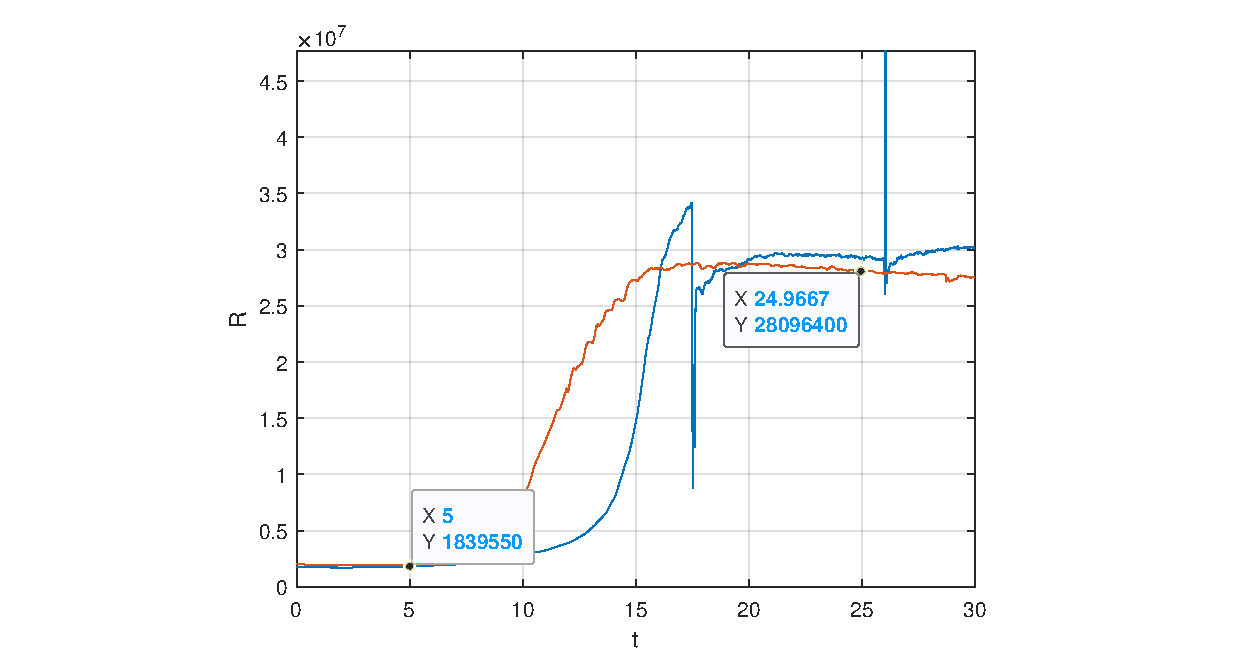
\includegraphics{./plots/full_1.pdf}}
	\end{center}
	\caption{Isolation full of water, isolation surface not wiped and needles stuck in the middle of the isolation}
	\label{fig:full_1}
\end{figure}

Second experiment was done as previous one with wet isolation, but this time needles were stuck to the top of isolation in order to not cross the inner hole what resulted in the \figurename{} \ref{fig:full_2}. There is huge diversity of the results in that experiments. Every particular test started from the same point, which is a couple of M$\Omega$ -- yellow curve for example in 5th minute shows a resistance on the level of 12M$\Omega$. After that 3 completely different thresholds were reached after growth till 20th minute. 

\begin{figure}[H]
	\begin{center}
		\scalebox{.7}{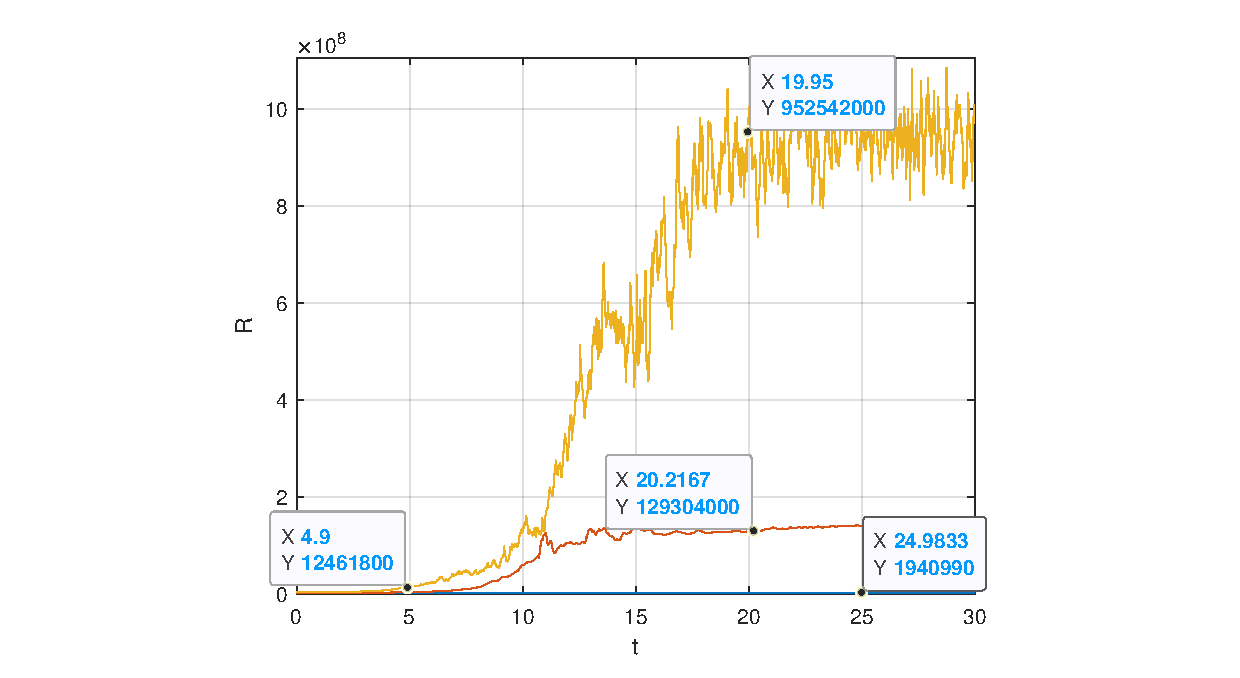
\includegraphics{./plots/full_2.pdf}}
	\end{center}
	\caption{Isolation full of water, isolation surface not wiped and needles stuck on the top of the isolation}
	\label{fig:full_2}
\end{figure}

Yellow curve stopped at 1G$\Omega$, orange one at 130M$\Omega$, which is really strange result and can be caused by some failure on the side of \verb|LTC| \verb|Meter|. Blue curve started at 350K$\Omega$ and reached limit of 2M$\Omega$. Conclusion from this experiment is following. In spite of potential failure with measuring device needles stuck to the top of isolation horizontally give very different results, caused by most likely different amount of water in the isolation and the gravitational issue explained during previous experiment. Top of the isolation is not good place to stick the needles.

\begin{figure}[H]
	\begin{center}
		\scalebox{.7}{% This file was created by matlab2tikz.
%
%The latest updates can be retrieved from
%  http://www.mathworks.com/matlabcentral/fileexchange/22022-matlab2tikz-matlab2tikz
%where you can also make suggestions and rate matlab2tikz.
%
\definecolor{mycolor1}{rgb}{0.00000,0.44700,0.74100}%
\definecolor{mycolor2}{rgb}{0.85000,0.32500,0.09800}%
\definecolor{mycolor3}{rgb}{0.92900,0.69400,0.12500}%
%
\begin{tikzpicture}

\begin{axis}[%
width=4.521in,
height=3.566in,
at={(0.758in,0.481in)},
scale only axis,
xmin=0,
xmax=30,
xlabel style={font=\color{white!15!black}},
xlabel={t},
ymin=-10000,
ymax=1216600,
ylabel style={font=\color{white!15!black}},
ylabel={R},
axis background/.style={fill=white},
xmajorgrids,
ymajorgrids,
legend style={at={(0.154,0.772)}, anchor=south west, legend cell align=left, align=left, draw=white!15!black}
]
\addplot [color=mycolor1]
  table[row sep=crcr]{%
0	488159\\
0.0166666666666667	487158\\
0.0333333333333333	486503\\
0.05	485421\\
0.0666666666666667	484555\\
0.0833333333333333	483652\\
0.1	482548\\
0.116666666666667	481559\\
0.133333333333333	480893\\
0.15	480098\\
0.166666666666667	479126\\
0.183333333333333	478315\\
0.2	477438\\
0.216666666666667	476676\\
0.233333333333333	475937\\
0.25	475174\\
0.266666666666667	474353\\
0.283333333333333	473755\\
0.3	473145\\
0.316666666666667	472559\\
0.333333333333333	472198\\
0.35	471754\\
0.366666666666667	471324\\
0.383333333333333	470878\\
0.4	470505\\
0.416666666666667	470349\\
0.433333333333333	470026\\
0.45	469780\\
0.466666666666667	469484\\
0.483333333333333	469126\\
0.5	468878\\
0.516666666666667	468517\\
0.533333333333333	468256\\
0.55	467968\\
0.566666666666667	467303\\
0.583333333333333	466725\\
0.6	466184\\
0.616666666666667	465922\\
0.633333333333333	465595\\
0.65	465254\\
0.666666666666667	464941\\
0.683333333333333	464859\\
0.7	465073\\
0.716666666666667	465035\\
0.733333333333333	464832\\
0.75	464655\\
0.766666666666667	464378\\
0.783333333333333	464146\\
0.8	463850\\
0.816666666666667	463418\\
0.833333333333333	463095\\
0.85	462812\\
0.866666666666667	462635\\
0.883333333333333	462431\\
0.9	462005\\
0.916666666666667	462093\\
0.933333333333333	461976\\
0.95	461887\\
0.966666666666667	461712\\
0.983333333333333	461352\\
1	461023\\
1.01666666666667	460805\\
1.03333333333333	460598\\
1.05	460395\\
1.06666666666667	460040\\
1.08333333333333	459880\\
1.1	459896\\
1.11666666666667	460043\\
1.13333333333333	460261\\
1.15	460159\\
1.16666666666667	460007\\
1.18333333333333	459792\\
1.2	459637\\
1.21666666666667	459527\\
1.23333333333333	459361\\
1.25	459222\\
1.26666666666667	459217\\
1.28333333333333	459407\\
1.3	459453\\
1.31666666666667	459423\\
1.33333333333333	459176\\
1.35	459126\\
1.36666666666667	459056\\
1.38333333333333	458994\\
1.4	458850\\
1.41666666666667	458999\\
1.43333333333333	458998\\
1.45	458962\\
1.46666666666667	458877\\
1.48333333333333	458902\\
1.5	459093\\
1.51666666666667	459366\\
1.53333333333333	459386\\
1.55	459250\\
1.56666666666667	459147\\
1.58333333333333	459155\\
1.6	459010\\
1.61666666666667	458815\\
1.63333333333333	458605\\
1.65	458502\\
1.66666666666667	458455\\
1.68333333333333	458410\\
1.7	458267\\
1.71666666666667	458009\\
1.73333333333333	457867\\
1.75	457883\\
1.76666666666667	457932\\
1.78333333333333	457915\\
1.8	457899\\
1.81666666666667	457769\\
1.83333333333333	457831\\
1.85	457856\\
1.86666666666667	458009\\
1.88333333333333	458174\\
1.9	458438\\
1.91666666666667	458518\\
1.93333333333333	458540\\
1.95	458599\\
1.96666666666667	458595\\
1.98333333333333	458608\\
2	458508\\
2.01666666666667	458326\\
2.03333333333333	458089\\
2.05	457952\\
2.06666666666667	457850\\
2.08333333333333	457974\\
2.1	458054\\
2.11666666666667	458055\\
2.13333333333333	458060\\
2.15	458171\\
2.16666666666667	458287\\
2.18333333333333	458448\\
2.2	458540\\
2.21666666666667	458678\\
2.23333333333333	458686\\
2.25	458638\\
2.26666666666667	458704\\
2.28333333333333	459195\\
2.3	459347\\
2.31666666666667	459418\\
2.33333333333333	459501\\
2.35	459425\\
2.36666666666667	459352\\
2.38333333333333	459368\\
2.4	459587\\
2.41666666666667	459766\\
2.43333333333333	459582\\
2.45	459372\\
2.46666666666667	459295\\
2.48333333333333	459156\\
2.5	458996\\
2.51666666666667	458826\\
2.53333333333333	458609\\
2.55	458423\\
2.56666666666667	458312\\
2.58333333333333	458276\\
2.6	458190\\
2.61666666666667	457734\\
2.63333333333333	457361\\
2.65	456954\\
2.66666666666667	456572\\
2.68333333333333	456230\\
2.7	455882\\
2.71666666666667	455586\\
2.73333333333333	455402\\
2.75	455233\\
2.76666666666667	455044\\
2.78333333333333	455100\\
2.8	455184\\
2.81666666666667	455163\\
2.83333333333333	455103\\
2.85	454965\\
2.86666666666667	454802\\
2.88333333333333	454646\\
2.9	454504\\
2.91666666666667	454399\\
2.93333333333333	454305\\
2.95	454195\\
2.96666666666667	454114\\
2.98333333333333	454029\\
3	453922\\
3.01666666666667	453840\\
3.03333333333333	453738\\
3.05	453625\\
3.06666666666667	453591\\
3.08333333333333	453596\\
3.1	453739\\
3.11666666666667	453864\\
3.13333333333333	453893\\
3.15	454067\\
3.16666666666667	454195\\
3.18333333333333	454516\\
3.2	454832\\
3.21666666666667	455027\\
3.23333333333333	455117\\
3.25	455174\\
3.26666666666667	455786\\
3.28333333333333	456440\\
3.3	456306\\
3.31666666666667	456239\\
3.33333333333333	456193\\
3.35	456237\\
3.36666666666667	456398\\
3.38333333333333	456603\\
3.4	456481\\
3.41666666666667	456385\\
3.43333333333333	456365\\
3.45	456335\\
3.46666666666667	456360\\
3.48333333333333	456437\\
3.5	456735\\
3.51666666666667	457346\\
3.53333333333333	457485\\
3.55	457389\\
3.56666666666667	457292\\
3.58333333333333	457303\\
3.6	457258\\
3.61666666666667	457215\\
3.63333333333333	457369\\
3.65	457634\\
3.66666666666667	457640\\
3.68333333333333	457567\\
3.7	457480\\
3.71666666666667	457519\\
3.73333333333333	457521\\
3.75	457531\\
3.76666666666667	457624\\
3.78333333333333	457697\\
3.8	457699\\
3.81666666666667	457559\\
3.83333333333333	457540\\
3.85	457431\\
3.86666666666667	457397\\
3.88333333333333	457424\\
3.9	457410\\
3.91666666666667	457297\\
3.93333333333333	457288\\
3.95	457427\\
3.96666666666667	457503\\
3.98333333333333	457536\\
4	457625\\
4.01666666666667	457727\\
4.03333333333333	457715\\
4.05	457764\\
4.06666666666667	458058\\
4.08333333333333	458356\\
4.1	458418\\
4.11666666666667	458565\\
4.13333333333333	458606\\
4.15	458645\\
4.16666666666667	458826\\
4.18333333333333	458846\\
4.2	458819\\
4.21666666666667	458800\\
4.23333333333333	458796\\
4.25	458774\\
4.26666666666667	458768\\
4.28333333333333	458823\\
4.3	458861\\
4.31666666666667	458780\\
4.33333333333333	458963\\
4.35	459238\\
4.36666666666667	459485\\
4.38333333333333	459805\\
4.4	460142\\
4.41666666666667	460417\\
4.43333333333333	460593\\
4.45	460844\\
4.46666666666667	460981\\
4.48333333333333	461052\\
4.5	461226\\
4.51666666666667	461224\\
4.53333333333333	461313\\
4.55	461341\\
4.56666666666667	461557\\
4.58333333333333	462114\\
4.6	462363\\
4.61666666666667	462477\\
4.63333333333333	462611\\
4.65	462938\\
4.66666666666667	463224\\
4.68333333333333	463577\\
4.7	463855\\
4.71666666666667	464031\\
4.73333333333333	464238\\
4.75	464424\\
4.76666666666667	464541\\
4.78333333333333	464629\\
4.8	464716\\
4.81666666666667	464824\\
4.83333333333333	464919\\
4.85	464987\\
4.86666666666667	465030\\
4.88333333333333	465061\\
4.9	465140\\
4.91666666666667	465265\\
4.93333333333333	465305\\
4.95	465414\\
4.96666666666667	465510\\
4.98333333333333	465731\\
5	465884\\
5.01666666666667	466022\\
5.03333333333333	466197\\
5.05	466469\\
5.06666666666667	466928\\
5.08333333333333	467043\\
5.1	467156\\
5.11666666666667	467318\\
5.13333333333333	467744\\
5.15	468317\\
5.16666666666667	468540\\
5.18333333333333	468608\\
5.2	468515\\
5.21666666666667	468548\\
5.23333333333333	468661\\
5.25	468675\\
5.26666666666667	468675\\
5.28333333333333	468742\\
5.3	468830\\
5.31666666666667	468878\\
5.33333333333333	468931\\
5.35	469020\\
5.36666666666667	469068\\
5.38333333333333	469081\\
5.4	469170\\
5.41666666666667	469195\\
5.43333333333333	469215\\
5.45	469261\\
5.46666666666667	469336\\
5.48333333333333	469426\\
5.5	469525\\
5.51666666666667	469625\\
5.53333333333333	469699\\
5.55	469762\\
5.56666666666667	469857\\
5.58333333333333	469965\\
5.6	469978\\
5.61666666666667	470073\\
5.63333333333333	470206\\
5.65	470385\\
5.66666666666667	470653\\
5.68333333333333	471097\\
5.7	471463\\
5.71666666666667	471696\\
5.73333333333333	471908\\
5.75	472100\\
5.76666666666667	472206\\
5.78333333333333	472248\\
5.8	472199\\
5.81666666666667	472301\\
5.83333333333333	472437\\
5.85	472482\\
5.86666666666667	472524\\
5.88333333333333	472625\\
5.9	472720\\
5.91666666666667	472851\\
5.93333333333333	473150\\
5.95	473391\\
5.96666666666667	473458\\
5.98333333333333	473419\\
6	473457\\
6.01666666666667	473778\\
6.03333333333333	474235\\
6.05	474426\\
6.06666666666667	474696\\
6.08333333333333	474809\\
6.1	474881\\
6.11666666666667	474935\\
6.13333333333333	474983\\
6.15	475280\\
6.16666666666667	475862\\
6.18333333333333	476421\\
6.2	477030\\
6.21666666666667	477357\\
6.23333333333333	477424\\
6.25	477422\\
6.26666666666667	477415\\
6.28333333333333	477318\\
6.3	477280\\
6.31666666666667	477292\\
6.33333333333333	477446\\
6.35	477467\\
6.36666666666667	477705\\
6.38333333333333	477658\\
6.4	477780\\
6.41666666666667	477925\\
6.43333333333333	477929\\
6.45	477969\\
6.46666666666667	478154\\
6.48333333333333	478250\\
6.5	478387\\
6.51666666666667	478578\\
6.53333333333333	478701\\
6.55	478816\\
6.56666666666667	479171\\
6.58333333333333	479408\\
6.6	479520\\
6.61666666666667	479768\\
6.63333333333333	479993\\
6.65	479871\\
6.66666666666667	479920\\
6.68333333333333	479935\\
6.7	480106\\
6.71666666666667	480485\\
6.73333333333333	480828\\
6.75	480971\\
6.76666666666667	481171\\
6.78333333333333	481287\\
6.8	481253\\
6.81666666666667	481281\\
6.83333333333333	481541\\
6.85	481972\\
6.86666666666667	482306\\
6.88333333333333	482586\\
6.9	482686\\
6.91666666666667	482651\\
6.93333333333333	482672\\
6.95	482813\\
6.96666666666667	483002\\
6.98333333333333	483168\\
7	483500\\
7.01666666666667	483841\\
7.03333333333333	484080\\
7.05	484417\\
7.06666666666667	484522\\
7.08333333333333	484657\\
7.1	484601\\
7.11666666666667	484519\\
7.13333333333333	484543\\
7.15	484649\\
7.16666666666667	484813\\
7.18333333333333	484975\\
7.2	485036\\
7.21666666666667	485191\\
7.23333333333333	485258\\
7.25	485391\\
7.26666666666667	485493\\
7.28333333333333	485520\\
7.3	485499\\
7.31666666666667	485452\\
7.33333333333333	485515\\
7.35	485522\\
7.36666666666667	485510\\
7.38333333333333	487737\\
7.4	487332\\
7.41666666666667	487470\\
7.43333333333333	487610\\
7.45	487916\\
7.46666666666667	488242\\
7.48333333333333	488317\\
7.5	488535\\
7.51666666666667	488789\\
7.53333333333333	488938\\
7.55	489050\\
7.56666666666667	489140\\
7.58333333333333	489253\\
7.6	489365\\
7.61666666666667	489474\\
7.63333333333333	489639\\
7.65	489906\\
7.66666666666667	490198\\
7.68333333333333	490530\\
7.7	490805\\
7.71666666666667	490881\\
7.73333333333333	490929\\
7.75	491368\\
7.76666666666667	491942\\
7.78333333333333	492020\\
7.8	492073\\
7.81666666666667	492284\\
7.83333333333333	492619\\
7.85	492840\\
7.86666666666667	492860\\
7.88333333333333	493018\\
7.9	493017\\
7.91666666666667	492987\\
7.93333333333333	492965\\
7.95	492957\\
7.96666666666667	492959\\
7.98333333333333	493032\\
8	493230\\
8.01666666666667	493482\\
8.03333333333333	493526\\
8.05	493528\\
8.06666666666667	493627\\
8.08333333333333	493851\\
8.1	494048\\
8.11666666666667	494160\\
8.13333333333333	494248\\
8.15	494388\\
8.16666666666667	494652\\
8.18333333333333	494901\\
8.2	495003\\
8.21666666666667	494999\\
8.23333333333333	495137\\
8.25	495263\\
8.26666666666667	495397\\
8.28333333333333	495595\\
8.3	495607\\
8.31666666666667	495847\\
8.33333333333333	495992\\
8.35	496045\\
8.36666666666667	496092\\
8.38333333333333	496100\\
8.4	496146\\
8.41666666666667	496189\\
8.43333333333333	496215\\
8.45	496298\\
8.46666666666667	496353\\
8.48333333333333	496348\\
8.5	496406\\
8.51666666666667	496653\\
8.53333333333333	496829\\
8.55	496862\\
8.56666666666667	496917\\
8.58333333333333	497109\\
8.6	497342\\
8.61666666666667	497478\\
8.63333333333333	497568\\
8.65	497717\\
8.66666666666667	497863\\
8.68333333333333	497882\\
8.7	497932\\
8.71666666666667	498105\\
8.73333333333333	498367\\
8.75	498560\\
8.76666666666667	498745\\
8.78333333333333	498938\\
8.8	498930\\
8.81666666666667	498872\\
8.83333333333333	498829\\
8.85	498873\\
8.86666666666667	498936\\
8.88333333333333	499058\\
8.9	499168\\
8.91666666666667	499457\\
8.93333333333333	499598\\
8.95	499622\\
8.96666666666667	500016\\
8.98333333333333	500173\\
9	500357\\
9.01666666666667	500775\\
9.03333333333333	501144\\
9.05	501516\\
9.06666666666667	501784\\
9.08333333333333	501727\\
9.1	501643\\
9.11666666666667	501559\\
9.13333333333333	501488\\
9.15	501476\\
9.16666666666667	501495\\
9.18333333333333	501524\\
9.2	501473\\
9.21666666666667	501498\\
9.23333333333333	501532\\
9.25	501547\\
9.26666666666667	501493\\
9.28333333333333	501532\\
9.3	501632\\
9.31666666666667	501722\\
9.33333333333333	501863\\
9.35	501979\\
9.36666666666667	502025\\
9.38333333333333	502030\\
9.4	502026\\
9.41666666666667	502065\\
9.43333333333333	502075\\
9.45	502098\\
9.46666666666667	502331\\
9.48333333333333	502514\\
9.5	502913\\
9.51666666666667	503314\\
9.53333333333333	503529\\
9.55	503927\\
9.56666666666667	504308\\
9.58333333333333	504413\\
9.6	504414\\
9.61666666666667	504368\\
9.63333333333333	504320\\
9.65	504264\\
9.66666666666667	504290\\
9.68333333333333	504285\\
9.7	504374\\
9.71666666666667	504475\\
9.73333333333333	504638\\
9.75	504674\\
9.76666666666667	504700\\
9.78333333333333	504858\\
9.8	504890\\
9.81666666666667	505026\\
9.83333333333333	505279\\
9.85	505603\\
9.86666666666667	505818\\
9.88333333333333	506005\\
9.9	506314\\
9.91666666666667	507071\\
9.93333333333333	507409\\
9.95	507538\\
9.96666666666667	507572\\
9.98333333333333	507882\\
10	508300\\
10.0166666666667	508713\\
10.0333333333333	509106\\
10.05	509363\\
10.0666666666667	509255\\
10.0833333333333	509050\\
10.1	508971\\
10.1166666666667	508978\\
10.1333333333333	508911\\
10.15	508941\\
10.1666666666667	508970\\
10.1833333333333	508981\\
10.2	508978\\
10.2166666666667	509022\\
10.2333333333333	508968\\
10.25	509259\\
10.2666666666667	509279\\
10.2833333333333	509210\\
10.3	509243\\
10.3166666666667	509223\\
10.3333333333333	509221\\
10.35	509211\\
10.3666666666667	509289\\
10.3833333333333	509432\\
10.4	509685\\
10.4166666666667	509762\\
10.4333333333333	509892\\
10.45	510098\\
10.4666666666667	510339\\
10.4833333333333	510697\\
10.5	510985\\
10.5166666666667	511501\\
10.5333333333333	511904\\
10.55	511790\\
10.5666666666667	511695\\
10.5833333333333	511591\\
10.6	511615\\
10.6166666666667	511623\\
10.6333333333333	511690\\
10.65	511820\\
10.6666666666667	511937\\
10.6833333333333	512067\\
10.7	512101\\
10.7166666666667	512087\\
10.7333333333333	512343\\
10.75	512589\\
10.7666666666667	513069\\
10.7833333333333	513559\\
10.8	513628\\
10.8166666666667	514029\\
10.8333333333333	514361\\
10.85	514132\\
10.8666666666667	513846\\
10.8833333333333	513697\\
10.9	513572\\
10.9166666666667	513387\\
10.9333333333333	513306\\
10.95	513187\\
10.9666666666667	513107\\
10.9833333333333	513073\\
11	513064\\
11.0166666666667	513114\\
11.0333333333333	513236\\
11.05	513390\\
11.0666666666667	513473\\
11.0833333333333	513600\\
11.1	513643\\
11.1166666666667	513700\\
11.1333333333333	513712\\
11.15	513720\\
11.1666666666667	513787\\
11.1833333333333	513866\\
11.2	513924\\
11.2166666666667	514018\\
11.2333333333333	514077\\
11.25	514065\\
11.2666666666667	514113\\
11.2833333333333	514245\\
11.3	514393\\
11.3166666666667	514477\\
11.3333333333333	514630\\
11.35	514649\\
11.3666666666667	514668\\
11.3833333333333	514712\\
11.4	514682\\
11.4166666666667	514770\\
11.4333333333333	514874\\
11.45	515068\\
11.4666666666667	515363\\
11.4833333333333	515518\\
11.5	515603\\
11.5166666666667	515630\\
11.5333333333333	515747\\
11.55	515768\\
11.5666666666667	515894\\
11.5833333333333	516039\\
11.6	516068\\
11.6166666666667	516097\\
11.6333333333333	516083\\
11.65	516095\\
11.6666666666667	516130\\
11.6833333333333	516282\\
11.7	516541\\
11.7166666666667	516899\\
11.7333333333333	517896\\
11.75	518162\\
11.7666666666667	518105\\
11.7833333333333	517998\\
11.8	518200\\
11.8166666666667	518329\\
11.8333333333333	518243\\
11.85	518228\\
11.8666666666667	518107\\
11.8833333333333	518045\\
11.9	517931\\
11.9166666666667	517862\\
11.9333333333333	518437\\
11.95	519022\\
11.9666666666667	518755\\
11.9833333333333	518660\\
12	518622\\
12.0166666666667	518566\\
12.0333333333333	518774\\
12.05	518807\\
12.0666666666667	518928\\
12.0833333333333	519131\\
12.1	519335\\
12.1166666666667	519394\\
12.1333333333333	519238\\
12.15	519243\\
12.1666666666667	519980\\
12.1833333333333	520070\\
12.2	520180\\
12.2166666666667	520295\\
12.2333333333333	520365\\
12.25	520489\\
12.2666666666667	520467\\
12.2833333333333	520517\\
12.3	520693\\
12.3166666666667	520838\\
12.3333333333333	520991\\
12.35	521115\\
12.3666666666667	520980\\
12.3833333333333	520849\\
12.4	520933\\
12.4166666666667	520966\\
12.4333333333333	520957\\
12.45	520988\\
12.4666666666667	521007\\
12.4833333333333	521084\\
12.5	521091\\
12.5166666666667	520999\\
12.5333333333333	521032\\
12.55	521116\\
12.5666666666667	521191\\
12.5833333333333	521367\\
12.6	521654\\
12.6166666666667	522015\\
12.6333333333333	522135\\
12.65	522141\\
12.6666666666667	522138\\
12.6833333333333	522114\\
12.7	522083\\
12.7166666666667	522132\\
12.7333333333333	522176\\
12.75	522296\\
12.7666666666667	522671\\
12.7833333333333	522972\\
12.8	523056\\
12.8166666666667	523026\\
12.8333333333333	523014\\
12.85	523047\\
12.8666666666667	523267\\
12.8833333333333	523361\\
12.9	523853\\
12.9166666666667	523781\\
12.9333333333333	523916\\
12.95	523776\\
12.9666666666667	523846\\
12.9833333333333	523764\\
13	523737\\
13.0166666666667	523700\\
13.0333333333333	523858\\
13.05	523993\\
13.0666666666667	524155\\
13.0833333333333	524201\\
13.1	524309\\
13.1166666666667	524435\\
13.1333333333333	524464\\
13.15	524554\\
13.1666666666667	524648\\
13.1833333333333	525173\\
13.2	525637\\
13.2166666666667	526042\\
13.2333333333333	526234\\
13.25	526215\\
13.2666666666667	526195\\
13.2833333333333	526157\\
13.3	526162\\
13.3166666666667	526733\\
13.3333333333333	527009\\
13.35	527122\\
13.3666666666667	527298\\
13.3833333333333	527212\\
13.4	526989\\
13.4166666666667	526789\\
13.4333333333333	526736\\
13.45	526746\\
13.4666666666667	526725\\
13.4833333333333	526803\\
13.5	526880\\
13.5166666666667	526912\\
13.5333333333333	526900\\
13.55	526867\\
13.5666666666667	527169\\
13.5833333333333	527195\\
13.6	527293\\
13.6166666666667	527432\\
13.6333333333333	527648\\
13.65	527676\\
13.6666666666667	527664\\
13.6833333333333	527647\\
13.7	527615\\
13.7166666666667	527698\\
13.7333333333333	527608\\
13.75	527546\\
13.7666666666667	527690\\
13.7833333333333	527705\\
13.8	527857\\
13.8166666666667	527961\\
13.8333333333333	528053\\
13.85	528101\\
13.8666666666667	528177\\
13.8833333333333	528203\\
13.9	528234\\
13.9166666666667	528312\\
13.9333333333333	528423\\
13.95	528615\\
13.9666666666667	528761\\
13.9833333333333	528886\\
14	528969\\
14.0166666666667	529113\\
14.0333333333333	529833\\
14.05	530837\\
14.0666666666667	531451\\
14.0833333333333	531261\\
14.1	531079\\
14.1166666666667	531115\\
14.1333333333333	531120\\
14.15	531227\\
14.1666666666667	531364\\
14.1833333333333	531494\\
14.2	531342\\
14.2166666666667	531180\\
14.2333333333333	531282\\
14.25	531508\\
14.2666666666667	531710\\
14.2833333333333	532019\\
14.3	532192\\
14.3166666666667	532484\\
14.3333333333333	532634\\
14.35	532692\\
14.3666666666667	532578\\
14.3833333333333	532527\\
14.4	532690\\
14.4166666666667	532788\\
14.4333333333333	532848\\
14.45	532851\\
14.4666666666667	532694\\
14.4833333333333	532426\\
14.5	532294\\
14.5166666666667	532404\\
14.5333333333333	532353\\
14.55	532278\\
14.5666666666667	532289\\
14.5833333333333	532192\\
14.6	532133\\
14.6166666666667	532154\\
14.6333333333333	532111\\
14.65	532196\\
14.6666666666667	532186\\
14.6833333333333	532271\\
14.7	532353\\
14.7166666666667	532319\\
14.7333333333333	532365\\
14.75	532447\\
14.7666666666667	532470\\
14.7833333333333	532380\\
14.8	532319\\
14.8166666666667	532140\\
14.8333333333333	532273\\
14.85	532266\\
14.8666666666667	532286\\
14.8833333333333	532270\\
14.9	532333\\
14.9166666666667	532427\\
14.9333333333333	532546\\
14.95	532683\\
14.9666666666667	532757\\
14.9833333333333	532901\\
15	532925\\
15.0166666666667	532954\\
15.0333333333333	532945\\
15.05	532876\\
15.0666666666667	533543\\
15.0833333333333	533791\\
15.1	534214\\
15.1166666666667	534210\\
15.1333333333333	534192\\
15.15	534319\\
15.1666666666667	534375\\
15.1833333333333	534581\\
15.2	534732\\
15.2166666666667	534613\\
15.2333333333333	534544\\
15.25	534480\\
15.2666666666667	534593\\
15.2833333333333	534736\\
15.3	534815\\
15.3166666666667	534892\\
15.3333333333333	534893\\
15.35	534827\\
15.3666666666667	534808\\
15.3833333333333	534863\\
15.4	534806\\
15.4166666666667	534807\\
15.4333333333333	534795\\
15.45	534820\\
15.4666666666667	535125\\
15.4833333333333	535222\\
15.5	535231\\
15.5166666666667	535426\\
15.5333333333333	535647\\
15.55	535740\\
15.5666666666667	535788\\
15.5833333333333	535810\\
15.6	535839\\
15.6166666666667	535848\\
15.6333333333333	535819\\
15.65	535815\\
15.6666666666667	535823\\
15.6833333333333	535904\\
15.7	536017\\
15.7166666666667	536162\\
15.7333333333333	536368\\
15.75	536409\\
15.7666666666667	536639\\
15.7833333333333	537179\\
15.8	537228\\
15.8166666666667	537450\\
15.8333333333333	537620\\
15.85	538106\\
15.8666666666667	538874\\
15.8833333333333	539099\\
15.9	539335\\
15.9166666666667	539129\\
15.9333333333333	538752\\
15.95	538484\\
15.9666666666667	538186\\
15.9833333333333	537802\\
16	537497\\
16.0166666666667	538006\\
16.0333333333333	537842\\
16.05	537612\\
16.0666666666667	537511\\
16.0833333333333	537438\\
16.1	537398\\
16.1166666666667	537494\\
16.1333333333333	537474\\
16.15	537642\\
16.1666666666667	537591\\
16.1833333333333	537541\\
16.2	537663\\
16.2166666666667	537691\\
16.2333333333333	537716\\
16.25	537819\\
16.2666666666667	537823\\
16.2833333333333	537847\\
16.3	538126\\
16.3166666666667	538497\\
16.3333333333333	538681\\
16.35	538444\\
16.3666666666667	538277\\
16.3833333333333	538128\\
16.4	538145\\
16.4166666666667	538126\\
16.4333333333333	538107\\
16.45	538307\\
16.4666666666667	538687\\
16.4833333333333	538930\\
16.5	539187\\
16.5166666666667	539403\\
16.5333333333333	539517\\
16.55	539668\\
16.5666666666667	539701\\
16.5833333333333	539558\\
16.6	539469\\
16.6166666666667	539492\\
16.6333333333333	539700\\
16.65	539753\\
16.6666666666667	539903\\
16.6833333333333	540046\\
16.7	540093\\
16.7166666666667	540117\\
16.7333333333333	540100\\
16.75	540162\\
16.7666666666667	540087\\
16.7833333333333	540201\\
16.8	540074\\
16.8166666666667	539999\\
16.8333333333333	539995\\
16.85	540021\\
16.8666666666667	540501\\
16.8833333333333	540721\\
16.9	540634\\
16.9166666666667	540653\\
16.9333333333333	540743\\
16.95	540894\\
16.9666666666667	541186\\
16.9833333333333	541132\\
17	540890\\
17.0166666666667	540765\\
17.0333333333333	540746\\
17.05	541186\\
17.0666666666667	541432\\
17.0833333333333	541605\\
17.1	541820\\
17.1166666666667	541955\\
17.1333333333333	542136\\
17.15	542491\\
17.1666666666667	542374\\
17.1833333333333	542116\\
17.2	542155\\
17.2166666666667	542269\\
17.2333333333333	542086\\
17.25	541759\\
17.2666666666667	541455\\
17.2833333333333	541238\\
17.3	541134\\
17.3166666666667	541079\\
17.3333333333333	540970\\
17.35	541065\\
17.3666666666667	541409\\
17.3833333333333	541604\\
17.4	541602\\
17.4166666666667	541752\\
17.4333333333333	541863\\
17.45	542315\\
17.4666666666667	542307\\
17.4833333333333	542284\\
17.5	542348\\
17.5166666666667	542151\\
17.5333333333333	542022\\
17.55	541877\\
17.5666666666667	541644\\
17.5833333333333	541563\\
17.6	541542\\
17.6166666666667	541591\\
17.6333333333333	541711\\
17.65	542029\\
17.6666666666667	542084\\
17.6833333333333	542321\\
17.7	542403\\
17.7166666666667	542199\\
17.7333333333333	542151\\
17.75	542141\\
17.7666666666667	542048\\
17.7833333333333	541837\\
17.8	541807\\
17.8166666666667	541845\\
17.8333333333333	541992\\
17.85	542019\\
17.8666666666667	542063\\
17.8833333333333	542065\\
17.9	542170\\
17.9166666666667	542104\\
17.9333333333333	542031\\
17.95	541998\\
17.9666666666667	541990\\
17.9833333333333	542042\\
18	542124\\
18.0166666666667	542324\\
18.0333333333333	542448\\
18.05	542474\\
18.0666666666667	542820\\
18.0833333333333	543869\\
18.1	544644\\
18.1166666666667	544929\\
18.1333333333333	544588\\
18.15	544137\\
18.1666666666667	543934\\
18.1833333333333	543803\\
18.2	543954\\
18.2166666666667	544022\\
18.2333333333333	543880\\
18.25	543746\\
18.2666666666667	544094\\
18.2833333333333	544523\\
18.3	544494\\
18.3166666666667	544528\\
18.3333333333333	544572\\
18.35	544349\\
18.3666666666667	544194\\
18.3833333333333	544154\\
18.4	544216\\
18.4166666666667	544473\\
18.4333333333333	544501\\
18.45	544977\\
18.4666666666667	545161\\
18.4833333333333	545103\\
18.5	545360\\
18.5166666666667	545391\\
18.5333333333333	545266\\
18.55	545134\\
18.5666666666667	545330\\
18.5833333333333	545774\\
18.6	545979\\
18.6166666666667	545752\\
18.6333333333333	545587\\
18.65	545546\\
18.6666666666667	545330\\
18.6833333333333	545230\\
18.7	545125\\
18.7166666666667	545038\\
18.7333333333333	544925\\
18.75	544842\\
18.7666666666667	544802\\
18.7833333333333	544758\\
18.8	544762\\
18.8166666666667	544826\\
18.8333333333333	545107\\
18.85	545150\\
18.8666666666667	545241\\
18.8833333333333	545262\\
18.9	545122\\
18.9166666666667	545213\\
18.9333333333333	545258\\
18.95	545200\\
18.9666666666667	545281\\
18.9833333333333	545463\\
19	545623\\
19.0166666666667	545570\\
19.0333333333333	545448\\
19.05	545443\\
19.0666666666667	545458\\
19.0833333333333	545470\\
19.1	545568\\
19.1166666666667	545637\\
19.1333333333333	545734\\
19.15	545858\\
19.1666666666667	546003\\
19.1833333333333	546195\\
19.2	546422\\
19.2166666666667	546714\\
19.2333333333333	546762\\
19.25	546736\\
19.2666666666667	546749\\
19.2833333333333	546647\\
19.3	546450\\
19.3166666666667	546435\\
19.3333333333333	546481\\
19.35	546602\\
19.3666666666667	546725\\
19.3833333333333	547011\\
19.4	547361\\
19.4166666666667	547837\\
19.4333333333333	548263\\
19.45	548510\\
19.4666666666667	548695\\
19.4833333333333	548836\\
19.5	548767\\
19.5166666666667	548499\\
19.5333333333333	548403\\
19.55	548381\\
19.5666666666667	548290\\
19.5833333333333	548282\\
19.6	548418\\
19.6166666666667	548775\\
19.6333333333333	549134\\
19.65	549333\\
19.6666666666667	549514\\
19.6833333333333	549726\\
19.7	549853\\
19.7166666666667	549746\\
19.7333333333333	549591\\
19.75	549358\\
19.7666666666667	549039\\
19.7833333333333	548882\\
19.8	548929\\
19.8166666666667	549227\\
19.8333333333333	549134\\
19.85	549058\\
19.8666666666667	549161\\
19.8833333333333	549091\\
19.9	548999\\
19.9166666666667	548883\\
19.9333333333333	549034\\
19.95	549211\\
19.9666666666667	549241\\
19.9833333333333	549043\\
20	549071\\
20.0166666666667	553417\\
20.0333333333333	552637\\
20.05	552373\\
20.0666666666667	552548\\
20.0833333333333	552467\\
20.1	552333\\
20.1166666666667	552298\\
20.1333333333333	552316\\
20.15	552372\\
20.1666666666667	552330\\
20.1833333333333	552356\\
20.2	552461\\
20.2166666666667	552619\\
20.2333333333333	552807\\
20.25	552758\\
20.2666666666667	552785\\
20.2833333333333	553005\\
20.3	553042\\
20.3166666666667	553310\\
20.3333333333333	553482\\
20.35	553866\\
20.3666666666667	553899\\
20.3833333333333	553992\\
20.4	553853\\
20.4166666666667	553929\\
20.4333333333333	554109\\
20.45	553911\\
20.4666666666667	553806\\
20.4833333333333	553883\\
20.5	553920\\
20.5166666666667	553854\\
20.5333333333333	553866\\
20.55	553909\\
20.5666666666667	554076\\
20.5833333333333	554402\\
20.6	554511\\
20.6166666666667	554748\\
20.6333333333333	555137\\
20.65	555440\\
20.6666666666667	555536\\
20.6833333333333	555697\\
20.7	555743\\
20.7166666666667	555771\\
20.7333333333333	555852\\
20.75	555989\\
20.7666666666667	556161\\
20.7833333333333	556287\\
20.8	556362\\
20.8166666666667	556571\\
20.8333333333333	556505\\
20.85	556482\\
20.8666666666667	556364\\
20.8833333333333	556265\\
20.9	556444\\
20.9166666666667	556960\\
20.9333333333333	557701\\
20.95	558191\\
20.9666666666667	558281\\
20.9833333333333	558508\\
21	558614\\
21.0166666666667	558670\\
21.0333333333333	558847\\
21.05	558789\\
21.0666666666667	558675\\
21.0833333333333	558580\\
21.1	558526\\
21.1166666666667	558629\\
21.1333333333333	558673\\
21.15	558666\\
21.1666666666667	558803\\
21.1833333333333	558883\\
21.2	558891\\
21.2166666666667	558963\\
21.2333333333333	559075\\
21.25	559202\\
21.2666666666667	559138\\
21.2833333333333	559213\\
21.3	559137\\
21.3166666666667	559154\\
21.3333333333333	559360\\
21.35	559526\\
21.3666666666667	559946\\
21.3833333333333	560308\\
21.4	560468\\
21.4166666666667	560677\\
21.4333333333333	560591\\
21.45	560768\\
21.4666666666667	560848\\
21.4833333333333	560686\\
21.5	560963\\
21.5166666666667	561284\\
21.5333333333333	561064\\
21.55	561422\\
21.5666666666667	561534\\
21.5833333333333	561570\\
21.6	561660\\
21.6166666666667	561829\\
21.6333333333333	561830\\
21.65	562010\\
21.6666666666667	562057\\
21.6833333333333	562180\\
21.7	562522\\
21.7166666666667	562647\\
21.7333333333333	562869\\
21.75	562887\\
21.7666666666667	563132\\
21.7833333333333	563504\\
21.8	563511\\
21.8166666666667	563558\\
21.8333333333333	563861\\
21.85	564072\\
21.8666666666667	563794\\
21.8833333333333	564529\\
21.9	565176\\
21.9166666666667	565204\\
21.9333333333333	565041\\
21.95	565074\\
21.9666666666667	565444\\
21.9833333333333	565816\\
22	565995\\
22.0166666666667	566147\\
22.0333333333333	566076\\
22.05	566327\\
22.0666666666667	566675\\
22.0833333333333	566926\\
22.1	567209\\
22.1166666666667	567645\\
22.1333333333333	567851\\
22.15	567856\\
22.1666666666667	567970\\
22.1833333333333	568145\\
22.2	568653\\
22.2166666666667	569250\\
22.2333333333333	569776\\
22.25	569895\\
22.2666666666667	569812\\
22.2833333333333	569834\\
22.3	569850\\
22.3166666666667	569884\\
22.3333333333333	570069\\
22.35	570629\\
22.3666666666667	570907\\
22.3833333333333	571127\\
22.4	571408\\
22.4166666666667	571577\\
22.4333333333333	571793\\
22.45	571890\\
22.4666666666667	572326\\
22.4833333333333	572555\\
22.5	573386\\
22.5166666666667	577574\\
22.5333333333333	579370\\
22.55	574982\\
22.5666666666667	574370\\
22.5833333333333	573728\\
22.6	573467\\
22.6166666666667	573842\\
22.6333333333333	573489\\
22.65	573504\\
22.6666666666667	573460\\
22.6833333333333	573679\\
22.7	573818\\
22.7166666666667	574630\\
22.7333333333333	575092\\
22.75	575278\\
22.7666666666667	575546\\
22.7833333333333	575870\\
22.8	575945\\
22.8166666666667	582518\\
22.8333333333333	576597\\
22.85	576667\\
22.8666666666667	575369\\
22.8833333333333	575869\\
22.9	579911\\
22.9166666666667	581948\\
22.9333333333333	583028\\
22.95	584030\\
22.9666666666667	584441\\
22.9833333333333	584789\\
23	585283\\
23.0166666666667	585315\\
23.0333333333333	581278\\
23.05	580249\\
23.0666666666667	579940\\
23.0833333333333	581574\\
23.1	582391\\
23.1166666666667	582896\\
23.1333333333333	583443\\
23.15	583581\\
23.1666666666667	583771\\
23.1833333333333	583816\\
23.2	583813\\
23.2166666666667	583973\\
23.2333333333333	584570\\
23.25	584708\\
23.2666666666667	584286\\
23.2833333333333	584843\\
23.3	585540\\
23.3166666666667	586866\\
23.3333333333333	587708\\
23.35	586452\\
23.3666666666667	585922\\
23.3833333333333	585767\\
23.4	585608\\
23.4166666666667	585425\\
23.4333333333333	585435\\
23.45	585435\\
23.4666666666667	585456\\
23.4833333333333	585428\\
23.5	586100\\
23.5166666666667	586798\\
23.5333333333333	587891\\
23.55	589097\\
23.5666666666667	590877\\
23.5833333333333	591051\\
23.6	591639\\
23.6166666666667	591920\\
23.6333333333333	592456\\
23.65	593034\\
23.6666666666667	593937\\
23.6833333333333	594671\\
23.7	595722\\
23.7166666666667	596230\\
23.7333333333333	596694\\
23.75	596939\\
23.7666666666667	597418\\
23.7833333333333	597739\\
23.8	597665\\
23.8166666666667	598179\\
23.8333333333333	598550\\
23.85	598482\\
23.8666666666667	598572\\
23.8833333333333	598519\\
23.9	598827\\
23.9166666666667	598887\\
23.9333333333333	599031\\
23.95	599324\\
23.9666666666667	599752\\
23.9833333333333	600534\\
24	601054\\
24.0166666666667	602013\\
24.0333333333333	602668\\
24.05	603403\\
24.0666666666667	604120\\
24.0833333333333	605149\\
24.1	605623\\
24.1166666666667	606451\\
24.1333333333333	607108\\
24.15	607534\\
24.1666666666667	607865\\
24.1833333333333	608822\\
24.2	610534\\
24.2166666666667	611794\\
24.2333333333333	612177\\
24.25	612940\\
24.2666666666667	613240\\
24.2833333333333	613143\\
24.3	613378\\
24.3166666666667	613580\\
24.3333333333333	613947\\
24.35	614147\\
24.3666666666667	614432\\
24.3833333333333	614801\\
24.4	615718\\
24.4166666666667	616727\\
24.4333333333333	617612\\
24.45	619044\\
24.4666666666667	619875\\
24.4833333333333	620862\\
24.5	622595\\
24.5166666666667	623680\\
24.5333333333333	624314\\
24.55	624762\\
24.5666666666667	625321\\
24.5833333333333	626404\\
24.6	626984\\
24.6166666666667	627857\\
24.6333333333333	628455\\
24.65	630344\\
24.6666666666667	630871\\
24.6833333333333	632399\\
24.7	632066\\
24.7166666666667	631912\\
24.7333333333333	631720\\
24.75	631711\\
24.7666666666667	631834\\
24.7833333333333	631916\\
24.8	631811\\
24.8166666666667	631859\\
24.8333333333333	631883\\
24.85	632171\\
24.8666666666667	632716\\
24.8833333333333	633187\\
24.9	633208\\
24.9166666666667	633298\\
24.9333333333333	633414\\
24.95	633222\\
24.9666666666667	633350\\
24.9833333333333	633509\\
25	633833\\
25.0166666666667	634278\\
25.0333333333333	635108\\
25.05	636481\\
25.0666666666667	637976\\
25.0833333333333	638853\\
25.1	639372\\
25.1166666666667	639266\\
25.1333333333333	639268\\
25.15	639366\\
25.1666666666667	640147\\
25.1833333333333	640645\\
25.2	641285\\
25.2166666666667	643198\\
25.2333333333333	643404\\
25.25	644608\\
25.2666666666667	645115\\
25.2833333333333	645987\\
25.3	646888\\
25.3166666666667	648079\\
25.3333333333333	649063\\
25.35	650334\\
25.3666666666667	651744\\
25.3833333333333	652864\\
25.4	654566\\
25.4166666666667	657208\\
25.4333333333333	659263\\
25.45	661761\\
25.4666666666667	663265\\
25.4833333333333	664013\\
25.5	664724\\
25.5166666666667	665667\\
25.5333333333333	666215\\
25.55	668263\\
25.5666666666667	670373\\
25.5833333333333	671498\\
25.6	671036\\
25.6166666666667	672758\\
25.6333333333333	675554\\
25.65	677328\\
25.6666666666667	679602\\
25.6833333333333	681582\\
25.7	682050\\
25.7166666666667	679986\\
25.7333333333333	678971\\
25.75	678691\\
25.7666666666667	678588\\
25.7833333333333	678622\\
25.8	679376\\
25.8166666666667	680676\\
25.8333333333333	682030\\
25.85	683659\\
25.8666666666667	685943\\
25.8833333333333	686556\\
25.9	687207\\
25.9166666666667	687358\\
25.9333333333333	687462\\
25.95	688378\\
25.9666666666667	690090\\
25.9833333333333	691658\\
26	692233\\
26.0166666666667	692805\\
26.0333333333333	692774\\
26.05	693397\\
26.0666666666667	693776\\
26.0833333333333	694681\\
26.1	696371\\
26.1166666666667	696539\\
26.1333333333333	697060\\
26.15	697721\\
26.1666666666667	698647\\
26.1833333333333	698434\\
26.2	698613\\
26.2166666666667	698446\\
26.2333333333333	698845\\
26.25	699123\\
26.2666666666667	699513\\
26.2833333333333	699988\\
26.3	700080\\
26.3166666666667	700248\\
26.3333333333333	700419\\
26.35	700162\\
26.3666666666667	700606\\
26.3833333333333	702900\\
26.4	702747\\
26.4166666666667	705348\\
26.4333333333333	708611\\
26.45	709413\\
26.4666666666667	710087\\
26.4833333333333	710592\\
26.5	712366\\
26.5166666666667	715048\\
26.5333333333333	716088\\
26.55	718831\\
26.5666666666667	721352\\
26.5833333333333	723166\\
26.6	725083\\
26.6166666666667	727774\\
26.6333333333333	728244\\
26.65	728627\\
26.6666666666667	729449\\
26.6833333333333	730174\\
26.7	731215\\
26.7166666666667	732236\\
26.7333333333333	733073\\
26.75	733449\\
26.7666666666667	734000\\
26.7833333333333	734093\\
26.8	735257\\
26.8166666666667	736259\\
26.8333333333333	737329\\
26.85	738013\\
26.8666666666667	738789\\
26.8833333333333	739374\\
26.9	739124\\
26.9166666666667	739306\\
26.9333333333333	745074\\
26.95	746650\\
26.9666666666667	747822\\
26.9833333333333	749573\\
27	751939\\
27.0166666666667	753557\\
27.0333333333333	754536\\
27.05	755361\\
27.0666666666667	755244\\
27.0833333333333	756035\\
27.1	756562\\
27.1166666666667	756842\\
27.1333333333333	758327\\
27.15	758719\\
27.1666666666667	759242\\
27.1833333333333	759562\\
27.2	761618\\
27.2166666666667	764625\\
27.2333333333333	766108\\
27.25	767145\\
27.2666666666667	768100\\
27.2833333333333	768760\\
27.3	768896\\
27.3166666666667	768791\\
27.3333333333333	769056\\
27.35	772867\\
27.3666666666667	777708\\
27.3833333333333	779379\\
27.4	781381\\
27.4166666666667	781701\\
27.4333333333333	782471\\
27.45	782801\\
27.4666666666667	782722\\
27.4833333333333	782889\\
27.5	782366\\
27.5166666666667	782092\\
27.5333333333333	781316\\
27.55	780619\\
27.5666666666667	780550\\
27.5833333333333	781294\\
27.6	781829\\
27.6166666666667	783579\\
27.6333333333333	788617\\
27.65	792515\\
27.6666666666667	795496\\
27.6833333333333	796188\\
27.7	796895\\
27.7166666666667	796458\\
27.7333333333333	796516\\
27.75	796889\\
27.7666666666667	796388\\
27.7833333333333	796197\\
27.8	798021\\
27.8166666666667	798320\\
27.8333333333333	799267\\
27.85	798009\\
27.8666666666667	803657\\
27.8833333333333	809163\\
27.9	811429\\
27.9166666666667	813274\\
27.9333333333333	814989\\
27.95	815616\\
27.9666666666667	815914\\
27.9833333333333	816693\\
28	815912\\
28.0166666666667	814006\\
28.0333333333333	812541\\
28.05	813233\\
28.0666666666667	818107\\
28.0833333333333	819280\\
28.1	819285\\
28.1166666666667	822757\\
28.1333333333333	826739\\
28.15	831442\\
28.1666666666667	833194\\
28.1833333333333	829372\\
28.2	829867\\
28.2166666666667	835533\\
28.2333333333333	838326\\
28.25	839067\\
28.2666666666667	842274\\
28.2833333333333	843590\\
28.3	842094\\
28.3166666666667	840346\\
28.3333333333333	841441\\
28.35	841042\\
28.3666666666667	840540\\
28.3833333333333	841953\\
28.4	844426\\
28.4166666666667	847439\\
28.4333333333333	851132\\
28.45	854067\\
28.4666666666667	856920\\
28.4833333333333	859879\\
28.5	860833\\
28.5166666666667	859707\\
28.5333333333333	858629\\
28.55	859684\\
28.5666666666667	859599\\
28.5833333333333	861206\\
28.6	862369\\
28.6166666666667	862119\\
28.6333333333333	863379\\
28.65	865858\\
28.6666666666667	865893\\
28.6833333333333	867440\\
28.7	870152\\
28.7166666666667	873891\\
28.7333333333333	878383\\
28.75	880708\\
28.7666666666667	880481\\
28.7833333333333	879883\\
28.8	879920\\
28.8166666666667	882628\\
28.8333333333333	887144\\
28.85	890406\\
28.8666666666667	892536\\
28.8833333333333	895936\\
28.9	896014\\
28.9166666666667	894745\\
28.9333333333333	896161\\
28.95	898565\\
28.9666666666667	901915\\
28.9833333333333	903633\\
29	903532\\
29.0166666666667	902814\\
29.0333333333333	899950\\
29.05	895202\\
29.0666666666667	890791\\
29.0833333333333	887349\\
29.1	884360\\
29.1166666666667	882122\\
29.1333333333333	880557\\
29.15	880417\\
29.1666666666667	884856\\
29.1833333333333	887652\\
29.2	887080\\
29.2166666666667	885553\\
29.2333333333333	882957\\
29.25	883731\\
29.2666666666667	885051\\
29.2833333333333	886457\\
29.3	886135\\
29.3166666666667	886772\\
29.3333333333333	890936\\
29.35	891395\\
29.3666666666667	894201\\
29.3833333333333	900190\\
29.4	903645\\
29.4166666666667	902609\\
29.4333333333333	903567\\
29.45	905741\\
29.4666666666667	906401\\
29.4833333333333	908653\\
29.5	907906\\
29.5166666666667	907188\\
29.5333333333333	905490\\
29.55	903782\\
29.5666666666667	901584\\
29.5833333333333	896226\\
29.6	892867\\
29.6166666666667	892903\\
29.6333333333333	895280\\
29.65	898205\\
29.6666666666667	899078\\
29.6833333333333	897396\\
29.7	895311\\
29.7166666666667	902250\\
29.7333333333333	904683\\
29.75	911524\\
29.7666666666667	911043\\
29.7833333333333	909229\\
29.8	906930\\
29.8166666666667	904949\\
29.8333333333333	903501\\
29.85	901820\\
29.8666666666667	900142\\
29.8833333333333	899479\\
29.9	898682\\
29.9166666666667	896711\\
29.9333333333333	894132\\
29.95	894459\\
29.9666666666667	893209\\
29.9833333333333	890526\\
};

\addplot [color=mycolor2]
  table[row sep=crcr]{%
0	548776\\
0.0166666666666667	549089\\
0.0333333333333333	549596\\
0.05	550278\\
0.0666666666666667	551554\\
0.0833333333333333	553215\\
0.1	554210\\
0.116666666666667	555976\\
0.133333333333333	556437\\
0.15	556807\\
0.166666666666667	557163\\
0.183333333333333	557635\\
0.2	557986\\
0.216666666666667	557740\\
0.233333333333333	557704\\
0.25	557668\\
0.266666666666667	557955\\
0.283333333333333	558126\\
0.3	558260\\
0.316666666666667	558414\\
0.333333333333333	558717\\
0.35	559077\\
0.366666666666667	559372\\
0.383333333333333	559856\\
0.4	560384\\
0.416666666666667	560982\\
0.433333333333333	561207\\
0.45	561580\\
0.466666666666667	561783\\
0.483333333333333	562757\\
0.5	563332\\
0.516666666666667	563347\\
0.533333333333333	563530\\
0.55	563984\\
0.566666666666667	564397\\
0.583333333333333	564643\\
0.6	564676\\
0.616666666666667	565006\\
0.633333333333333	565443\\
0.65	565778\\
0.666666666666667	566414\\
0.683333333333333	567169\\
0.7	567676\\
0.716666666666667	568170\\
0.733333333333333	568680\\
0.75	569197\\
0.766666666666667	569749\\
0.783333333333333	570261\\
0.8	570678\\
0.816666666666667	571125\\
0.833333333333333	571500\\
0.85	572041\\
0.866666666666667	574167\\
0.883333333333333	575506\\
0.9	575746\\
0.916666666666667	577683\\
0.933333333333333	579022\\
0.95	579787\\
0.966666666666667	580556\\
0.983333333333333	580830\\
1	581741\\
1.01666666666667	582806\\
1.03333333333333	582954\\
1.05	583344\\
1.06666666666667	583875\\
1.08333333333333	584343\\
1.1	584852\\
1.11666666666667	585172\\
1.13333333333333	586745\\
1.15	587277\\
1.16666666666667	587531\\
1.18333333333333	587837\\
1.2	588092\\
1.21666666666667	588323\\
1.23333333333333	588310\\
1.25	588460\\
1.26666666666667	588824\\
1.28333333333333	589343\\
1.3	589857\\
1.31666666666667	590283\\
1.33333333333333	593224\\
1.35	595149\\
1.36666666666667	595915\\
1.38333333333333	596615\\
1.4	597284\\
1.41666666666667	598104\\
1.43333333333333	598944\\
1.45	599572\\
1.46666666666667	599947\\
1.48333333333333	600310\\
1.5	600755\\
1.51666666666667	601180\\
1.53333333333333	601653\\
1.55	602253\\
1.56666666666667	613317\\
1.58333333333333	618443\\
1.6	620609\\
1.61666666666667	622285\\
1.63333333333333	623557\\
1.65	624544\\
1.66666666666667	625339\\
1.68333333333333	626145\\
1.7	627071\\
1.71666666666667	628097\\
1.73333333333333	629179\\
1.75	632568\\
1.76666666666667	633363\\
1.78333333333333	634390\\
1.8	635422\\
1.81666666666667	636097\\
1.83333333333333	636565\\
1.85	637112\\
1.86666666666667	637821\\
1.88333333333333	638748\\
1.9	640198\\
1.91666666666667	641090\\
1.93333333333333	642592\\
1.95	643010\\
1.96666666666667	643270\\
1.98333333333333	645021\\
2	645344\\
2.01666666666667	646013\\
2.03333333333333	646642\\
2.05	647641\\
2.06666666666667	648269\\
2.08333333333333	649041\\
2.1	649783\\
2.11666666666667	650083\\
2.13333333333333	650710\\
2.15	651165\\
2.16666666666667	651638\\
2.18333333333333	652216\\
2.2	652634\\
2.21666666666667	653072\\
2.23333333333333	653755\\
2.25	654368\\
2.26666666666667	654663\\
2.28333333333333	656324\\
2.3	656881\\
2.31666666666667	657235\\
2.33333333333333	657578\\
2.35	657833\\
2.36666666666667	658244\\
2.38333333333333	658612\\
2.4	659018\\
2.41666666666667	659280\\
2.43333333333333	659731\\
2.45	660238\\
2.46666666666667	660575\\
2.48333333333333	661185\\
2.5	661457\\
2.51666666666667	661952\\
2.53333333333333	662576\\
2.55	664125\\
2.56666666666667	664963\\
2.58333333333333	666721\\
2.6	667053\\
2.61666666666667	667425\\
2.63333333333333	667784\\
2.65	667853\\
2.66666666666667	668508\\
2.68333333333333	669934\\
2.7	670598\\
2.71666666666667	670795\\
2.73333333333333	671470\\
2.75	671612\\
2.76666666666667	672200\\
2.78333333333333	672534\\
2.8	673021\\
2.81666666666667	672861\\
2.83333333333333	672680\\
2.85	673069\\
2.86666666666667	673109\\
2.88333333333333	673062\\
2.9	673153\\
2.91666666666667	673401\\
2.93333333333333	673422\\
2.95	673692\\
2.96666666666667	673746\\
2.98333333333333	670783\\
3	668507\\
3.01666666666667	668329\\
3.03333333333333	668372\\
3.05	668393\\
3.06666666666667	668402\\
3.08333333333333	668493\\
3.1	668669\\
3.11666666666667	668931\\
3.13333333333333	669199\\
3.15	669400\\
3.16666666666667	669669\\
3.18333333333333	669863\\
3.2	670590\\
3.21666666666667	670886\\
3.23333333333333	671029\\
3.25	671232\\
3.26666666666667	671409\\
3.28333333333333	671732\\
3.3	674308\\
3.31666666666667	674645\\
3.33333333333333	674931\\
3.35	675390\\
3.36666666666667	675961\\
3.38333333333333	676097\\
3.4	676217\\
3.41666666666667	676524\\
3.43333333333333	677017\\
3.45	677287\\
3.46666666666667	677269\\
3.48333333333333	677419\\
3.5	677484\\
3.51666666666667	677763\\
3.53333333333333	678146\\
3.55	678457\\
3.56666666666667	678802\\
3.58333333333333	679276\\
3.6	679745\\
3.61666666666667	680967\\
3.63333333333333	681223\\
3.65	681737\\
3.66666666666667	682505\\
3.68333333333333	682894\\
3.7	682938\\
3.71666666666667	682846\\
3.73333333333333	683145\\
3.75	683874\\
3.76666666666667	684384\\
3.78333333333333	684755\\
3.8	684988\\
3.81666666666667	685309\\
3.83333333333333	685830\\
3.85	685941\\
3.86666666666667	685787\\
3.88333333333333	685839\\
3.9	686067\\
3.91666666666667	686076\\
3.93333333333333	686218\\
3.95	686937\\
3.96666666666667	686865\\
3.98333333333333	687317\\
4	687788\\
4.01666666666667	688107\\
4.03333333333333	688406\\
4.05	688735\\
4.06666666666667	688886\\
4.08333333333333	689168\\
4.1	689308\\
4.11666666666667	689778\\
4.13333333333333	690339\\
4.15	690951\\
4.16666666666667	691603\\
4.18333333333333	691889\\
4.2	692298\\
4.21666666666667	692693\\
4.23333333333333	692988\\
4.25	693327\\
4.26666666666667	693676\\
4.28333333333333	693926\\
4.3	694295\\
4.31666666666667	694712\\
4.33333333333333	694755\\
4.35	694993\\
4.36666666666667	698092\\
4.38333333333333	698480\\
4.4	698672\\
4.41666666666667	698607\\
4.43333333333333	699041\\
4.45	700296\\
4.46666666666667	700882\\
4.48333333333333	701896\\
4.5	701896\\
4.51666666666667	701878\\
4.53333333333333	701887\\
4.55	701850\\
4.56666666666667	701939\\
4.58333333333333	702028\\
4.6	702158\\
4.61666666666667	702380\\
4.63333333333333	702294\\
4.65	702428\\
4.66666666666667	702705\\
4.68333333333333	703068\\
4.7	703676\\
4.71666666666667	704006\\
4.73333333333333	704019\\
4.75	704244\\
4.76666666666667	704302\\
4.78333333333333	704317\\
4.8	704315\\
4.81666666666667	704331\\
4.83333333333333	704359\\
4.85	704335\\
4.86666666666667	704321\\
4.88333333333333	704461\\
4.9	704478\\
4.91666666666667	704558\\
4.93333333333333	704551\\
4.95	704324\\
4.96666666666667	704237\\
4.98333333333333	704288\\
5	704375\\
5.01666666666667	704483\\
5.03333333333333	704615\\
5.05	704701\\
5.06666666666667	704855\\
5.08333333333333	705036\\
5.1	705330\\
5.11666666666667	705081\\
5.13333333333333	704139\\
5.15	704716\\
5.16666666666667	705113\\
5.18333333333333	705506\\
5.2	705812\\
5.21666666666667	705871\\
5.23333333333333	705883\\
5.25	705925\\
5.26666666666667	706530\\
5.28333333333333	707939\\
5.3	709116\\
5.31666666666667	709520\\
5.33333333333333	709511\\
5.35	709712\\
5.36666666666667	709806\\
5.38333333333333	709870\\
5.4	709874\\
5.41666666666667	709812\\
5.43333333333333	709922\\
5.45	710178\\
5.46666666666667	710248\\
5.48333333333333	710389\\
5.5	710525\\
5.51666666666667	710770\\
5.53333333333333	710848\\
5.55	710894\\
5.56666666666667	710952\\
5.58333333333333	711228\\
5.6	711464\\
5.61666666666667	711484\\
5.63333333333333	711369\\
5.65	711460\\
5.66666666666667	711899\\
5.68333333333333	712315\\
5.7	712605\\
5.71666666666667	713061\\
5.73333333333333	713363\\
5.75	713450\\
5.76666666666667	713661\\
5.78333333333333	713685\\
5.8	713603\\
5.81666666666667	713626\\
5.83333333333333	713631\\
5.85	713665\\
5.86666666666667	713648\\
5.88333333333333	713837\\
5.9	714112\\
5.91666666666667	714417\\
5.93333333333333	714498\\
5.95	714615\\
5.96666666666667	714945\\
5.98333333333333	715210\\
6	715468\\
6.01666666666667	716249\\
6.03333333333333	716562\\
6.05	717209\\
6.06666666666667	718791\\
6.08333333333333	717839\\
6.1	717903\\
6.11666666666667	718029\\
6.13333333333333	718238\\
6.15	718373\\
6.16666666666667	718409\\
6.18333333333333	718565\\
6.2	718743\\
6.21666666666667	718757\\
6.23333333333333	718830\\
6.25	719037\\
6.26666666666667	719368\\
6.28333333333333	719668\\
6.3	719820\\
6.31666666666667	719896\\
6.33333333333333	720207\\
6.35	720330\\
6.36666666666667	720557\\
6.38333333333333	721142\\
6.4	721222\\
6.41666666666667	720961\\
6.43333333333333	721064\\
6.45	721599\\
6.46666666666667	721709\\
6.48333333333333	721821\\
6.5	722121\\
6.51666666666667	722811\\
6.53333333333333	723097\\
6.55	723376\\
6.56666666666667	723425\\
6.58333333333333	723560\\
6.6	723739\\
6.61666666666667	723852\\
6.63333333333333	723818\\
6.65	724456\\
6.66666666666667	725510\\
6.68333333333333	725869\\
6.7	726155\\
6.71666666666667	726154\\
6.73333333333333	726076\\
6.75	726026\\
6.76666666666667	726444\\
6.78333333333333	726654\\
6.8	726796\\
6.81666666666667	726976\\
6.83333333333333	726979\\
6.85	726893\\
6.86666666666667	727026\\
6.88333333333333	727367\\
6.9	727885\\
6.91666666666667	728045\\
6.93333333333333	728375\\
6.95	733120\\
6.96666666666667	733497\\
6.98333333333333	733049\\
7	732625\\
7.01666666666667	732430\\
7.03333333333333	732317\\
7.05	732084\\
7.06666666666667	731987\\
7.08333333333333	732077\\
7.1	732562\\
7.11666666666667	732770\\
7.13333333333333	732985\\
7.15	733247\\
7.16666666666667	733531\\
7.18333333333333	733728\\
7.2	734600\\
7.21666666666667	734201\\
7.23333333333333	733829\\
7.25	734302\\
7.26666666666667	733971\\
7.28333333333333	733810\\
7.3	734048\\
7.31666666666667	733977\\
7.33333333333333	734069\\
7.35	734180\\
7.36666666666667	734254\\
7.38333333333333	734173\\
7.4	734225\\
7.41666666666667	734456\\
7.43333333333333	734394\\
7.45	734505\\
7.46666666666667	734742\\
7.48333333333333	735074\\
7.5	735188\\
7.51666666666667	735276\\
7.53333333333333	735375\\
7.55	735555\\
7.56666666666667	735579\\
7.58333333333333	735722\\
7.6	735685\\
7.61666666666667	735507\\
7.63333333333333	735443\\
7.65	735391\\
7.66666666666667	735415\\
7.68333333333333	735453\\
7.7	735548\\
7.71666666666667	735582\\
7.73333333333333	735676\\
7.75	736032\\
7.76666666666667	736411\\
7.78333333333333	736487\\
7.8	736652\\
7.81666666666667	736785\\
7.83333333333333	736774\\
7.85	736924\\
7.86666666666667	737118\\
7.88333333333333	737264\\
7.9	737494\\
7.91666666666667	737521\\
7.93333333333333	737534\\
7.95	737562\\
7.96666666666667	738337\\
7.98333333333333	739461\\
8	739649\\
8.01666666666667	739747\\
8.03333333333333	739853\\
8.05	740165\\
8.06666666666667	740425\\
8.08333333333333	740390\\
8.1	740498\\
8.11666666666667	740667\\
8.13333333333333	740532\\
8.15	740270\\
8.16666666666667	740026\\
8.18333333333333	739827\\
8.2	739911\\
8.21666666666667	739979\\
8.23333333333333	739952\\
8.25	739978\\
8.26666666666667	739919\\
8.28333333333333	740017\\
8.3	740073\\
8.31666666666667	740026\\
8.33333333333333	740203\\
8.35	740382\\
8.36666666666667	740905\\
8.38333333333333	741185\\
8.4	741254\\
8.41666666666667	741487\\
8.43333333333333	741628\\
8.45	741803\\
8.46666666666667	741773\\
8.48333333333333	741849\\
8.5	742829\\
8.51666666666667	743097\\
8.53333333333333	743685\\
8.55	744332\\
8.56666666666667	744320\\
8.58333333333333	744182\\
8.6	744108\\
8.61666666666667	744329\\
8.63333333333333	744608\\
8.65	744612\\
8.66666666666667	744424\\
8.68333333333333	744340\\
8.7	744465\\
8.71666666666667	744506\\
8.73333333333333	744594\\
8.75	744466\\
8.76666666666667	745301\\
8.78333333333333	745695\\
8.8	745700\\
8.81666666666667	745668\\
8.83333333333333	745643\\
8.85	745794\\
8.86666666666667	746311\\
8.88333333333333	746429\\
8.9	746572\\
8.91666666666667	746330\\
8.93333333333333	746240\\
8.95	746238\\
8.96666666666667	746344\\
8.98333333333333	746621\\
9	746681\\
9.01666666666667	746575\\
9.03333333333333	746741\\
9.05	746654\\
9.06666666666667	746815\\
9.08333333333333	746668\\
9.1	747399\\
9.11666666666667	748128\\
9.13333333333333	748441\\
9.15	749083\\
9.16666666666667	749123\\
9.18333333333333	749331\\
9.2	749287\\
9.21666666666667	749027\\
9.23333333333333	749133\\
9.25	749301\\
9.26666666666667	749150\\
9.28333333333333	748442\\
9.3	748034\\
9.31666666666667	747822\\
9.33333333333333	747662\\
9.35	748091\\
9.36666666666667	748265\\
9.38333333333333	748778\\
9.4	748691\\
9.41666666666667	748485\\
9.43333333333333	748345\\
9.45	748259\\
9.46666666666667	748134\\
9.48333333333333	748452\\
9.5	748651\\
9.51666666666667	749519\\
9.53333333333333	749707\\
9.55	749579\\
9.56666666666667	749440\\
9.58333333333333	749498\\
9.6	749831\\
9.61666666666667	749776\\
9.63333333333333	749959\\
9.65	750228\\
9.66666666666667	750350\\
9.68333333333333	750411\\
9.7	750491\\
9.71666666666667	750831\\
9.73333333333333	751303\\
9.75	751579\\
9.76666666666667	751701\\
9.78333333333333	752100\\
9.8	753008\\
9.81666666666667	753664\\
9.83333333333333	753616\\
9.85	753559\\
9.86666666666667	753553\\
9.88333333333333	753719\\
9.9	754402\\
9.91666666666667	754762\\
9.93333333333333	754455\\
9.95	754261\\
9.96666666666667	754122\\
9.98333333333333	754114\\
10	754158\\
10.0166666666667	754175\\
10.0333333333333	754166\\
10.05	754304\\
10.0666666666667	754429\\
10.0833333333333	754515\\
10.1	754757\\
10.1166666666667	754802\\
10.1333333333333	754712\\
10.15	754734\\
10.1666666666667	754756\\
10.1833333333333	754685\\
10.2	754765\\
10.2166666666667	755712\\
10.2333333333333	755943\\
10.25	755869\\
10.2666666666667	755942\\
10.2833333333333	756050\\
10.3	756101\\
10.3166666666667	756121\\
10.3333333333333	755968\\
10.35	756030\\
10.3666666666667	756326\\
10.3833333333333	756642\\
10.4	757040\\
10.4166666666667	757752\\
10.4333333333333	757982\\
10.45	757910\\
10.4666666666667	758357\\
10.4833333333333	758933\\
10.5	759039\\
10.5166666666667	759921\\
10.5333333333333	759741\\
10.55	760893\\
10.5666666666667	761381\\
10.5833333333333	762327\\
10.6	762367\\
10.6166666666667	762396\\
10.6333333333333	762296\\
10.65	762303\\
10.6666666666667	762119\\
10.6833333333333	761668\\
10.7	761907\\
10.7166666666667	762048\\
10.7333333333333	762363\\
10.75	762456\\
10.7666666666667	762408\\
10.7833333333333	762601\\
10.8	762780\\
10.8166666666667	763144\\
10.8333333333333	763281\\
10.85	763606\\
10.8666666666667	763332\\
10.8833333333333	763034\\
10.9	762942\\
10.9166666666667	763101\\
10.9333333333333	762767\\
10.95	762624\\
10.9666666666667	764435\\
10.9833333333333	764385\\
11	764720\\
11.0166666666667	765244\\
11.0333333333333	766001\\
11.05	766101\\
11.0666666666667	766114\\
11.0833333333333	766303\\
11.1	766569\\
11.1166666666667	766550\\
11.1333333333333	766602\\
11.15	766648\\
11.1666666666667	766743\\
11.1833333333333	766956\\
11.2	767113\\
11.2166666666667	767543\\
11.2333333333333	767729\\
11.25	767616\\
11.2666666666667	767225\\
11.2833333333333	766928\\
11.3	766624\\
11.3166666666667	766234\\
11.3333333333333	765926\\
11.35	765890\\
11.3666666666667	766307\\
11.3833333333333	766154\\
11.4	766175\\
11.4166666666667	765734\\
11.4333333333333	764535\\
11.45	763974\\
11.4666666666667	764733\\
11.4833333333333	765481\\
11.5	765291\\
11.5166666666667	764922\\
11.5333333333333	764951\\
11.55	766413\\
11.5666666666667	767691\\
11.5833333333333	767472\\
11.6	767301\\
11.6166666666667	766903\\
11.6333333333333	766701\\
11.65	766714\\
11.6666666666667	766609\\
11.6833333333333	766622\\
11.7	766604\\
11.7166666666667	766639\\
11.7333333333333	766600\\
11.75	766629\\
11.7666666666667	765467\\
11.7833333333333	765048\\
11.8	766600\\
11.8166666666667	767692\\
11.8333333333333	767979\\
11.85	767509\\
11.8666666666667	767262\\
11.8833333333333	766929\\
11.9	766573\\
11.9166666666667	766838\\
11.9333333333333	767308\\
11.95	767505\\
11.9666666666667	767593\\
11.9833333333333	767460\\
12	767427\\
12.0166666666667	767075\\
12.0333333333333	766924\\
12.05	766541\\
12.0666666666667	767291\\
12.0833333333333	767596\\
12.1	767607\\
12.1166666666667	767385\\
12.1333333333333	767431\\
12.15	767543\\
12.1666666666667	767473\\
12.1833333333333	767622\\
12.2	767581\\
12.2166666666667	768658\\
12.2333333333333	768787\\
12.25	768931\\
12.2666666666667	769246\\
12.2833333333333	769913\\
12.3	770092\\
12.3166666666667	769955\\
12.3333333333333	770043\\
12.35	770028\\
12.3666666666667	769169\\
12.3833333333333	768132\\
12.4	768314\\
12.4166666666667	768181\\
12.4333333333333	768095\\
12.45	768168\\
12.4666666666667	768334\\
12.4833333333333	768005\\
12.5	768101\\
12.5166666666667	768144\\
12.5333333333333	768280\\
12.55	769255\\
12.5666666666667	770413\\
12.5833333333333	771007\\
12.6	771351\\
12.6166666666667	771439\\
12.6333333333333	771605\\
12.65	771302\\
12.6666666666667	771066\\
12.6833333333333	770630\\
12.7	770160\\
12.7166666666667	770007\\
12.7333333333333	769890\\
12.75	770163\\
12.7666666666667	770811\\
12.7833333333333	770895\\
12.8	770783\\
12.8166666666667	770646\\
12.8333333333333	771251\\
12.85	771686\\
12.8666666666667	771698\\
12.8833333333333	771576\\
12.9	771359\\
12.9166666666667	771444\\
12.9333333333333	771571\\
12.95	771641\\
12.9666666666667	771855\\
12.9833333333333	771849\\
13	771699\\
13.0166666666667	771503\\
13.0333333333333	771411\\
13.05	771534\\
13.0666666666667	771399\\
13.0833333333333	771229\\
13.1	771197\\
13.1166666666667	771000\\
13.1333333333333	772207\\
13.15	773557\\
13.1666666666667	773979\\
13.1833333333333	774012\\
13.2	773912\\
13.2166666666667	773904\\
13.2333333333333	774112\\
13.25	774189\\
13.2666666666667	774250\\
13.2833333333333	774604\\
13.3	773855\\
13.3166666666667	774008\\
13.3333333333333	773952\\
13.35	773680\\
13.3666666666667	773400\\
13.3833333333333	773528\\
13.4	773780\\
13.4166666666667	774433\\
13.4333333333333	774988\\
13.45	775368\\
13.4666666666667	775152\\
13.4833333333333	774959\\
13.5	774693\\
13.5166666666667	774325\\
13.5333333333333	773941\\
13.55	773938\\
13.5666666666667	773784\\
13.5833333333333	774105\\
13.6	774478\\
13.6166666666667	774923\\
13.6333333333333	775151\\
13.65	775195\\
13.6666666666667	775061\\
13.6833333333333	775031\\
13.7	775003\\
13.7166666666667	775436\\
13.7333333333333	775650\\
13.75	775768\\
13.7666666666667	775566\\
13.7833333333333	775445\\
13.8	775390\\
13.8166666666667	775572\\
13.8333333333333	776091\\
13.85	776166\\
13.8666666666667	776336\\
13.8833333333333	776032\\
13.9	775818\\
13.9166666666667	775768\\
13.9333333333333	776120\\
13.95	776337\\
13.9666666666667	776632\\
13.9833333333333	777262\\
14	779726\\
14.0166666666667	780132\\
14.0333333333333	779825\\
14.05	779821\\
14.0666666666667	780047\\
14.0833333333333	780007\\
14.1	780156\\
14.1166666666667	780146\\
14.1333333333333	779869\\
14.15	779426\\
14.1666666666667	779121\\
14.1833333333333	779406\\
14.2	779882\\
14.2166666666667	780259\\
14.2333333333333	780453\\
14.25	780665\\
14.2666666666667	780884\\
14.2833333333333	780718\\
14.3	780663\\
14.3166666666667	780831\\
14.3333333333333	780782\\
14.35	780717\\
14.3666666666667	780698\\
14.3833333333333	781116\\
14.4	781385\\
14.4166666666667	781603\\
14.4333333333333	781532\\
14.45	781610\\
14.4666666666667	781850\\
14.4833333333333	781942\\
14.5	782348\\
14.5166666666667	783278\\
14.5333333333333	784016\\
14.55	784965\\
14.5666666666667	785449\\
14.5833333333333	785280\\
14.6	784947\\
14.6166666666667	784911\\
14.6333333333333	784826\\
14.65	784515\\
14.6666666666667	784813\\
14.6833333333333	784862\\
14.7	785079\\
14.7166666666667	785611\\
14.7333333333333	785895\\
14.75	786405\\
14.7666666666667	786663\\
14.7833333333333	786928\\
14.8	787185\\
14.8166666666667	787287\\
14.8333333333333	787390\\
14.85	787412\\
14.8666666666667	787425\\
14.8833333333333	787428\\
14.9	787509\\
14.9166666666667	786710\\
14.9333333333333	786940\\
14.95	787312\\
14.9666666666667	787333\\
14.9833333333333	787214\\
15	787132\\
15.0166666666667	787130\\
15.0333333333333	786981\\
15.05	787071\\
15.0666666666667	787399\\
15.0833333333333	787576\\
15.1	788129\\
15.1166666666667	788034\\
15.1333333333333	788448\\
15.15	788807\\
15.1666666666667	788709\\
15.1833333333333	789787\\
15.2	790748\\
15.2166666666667	790934\\
15.2333333333333	790962\\
15.25	790934\\
15.2666666666667	791229\\
15.2833333333333	791116\\
15.3	791227\\
15.3166666666667	791313\\
15.3333333333333	791202\\
15.35	791238\\
15.3666666666667	791157\\
15.3833333333333	791159\\
15.4	791555\\
15.4166666666667	791388\\
15.4333333333333	786905\\
15.45	787813\\
15.4666666666667	788478\\
15.4833333333333	788718\\
15.5	788848\\
15.5166666666667	789249\\
15.5333333333333	789795\\
15.55	790111\\
15.5666666666667	790817\\
15.5833333333333	791303\\
15.6	791211\\
15.6166666666667	790985\\
15.6333333333333	791002\\
15.65	791219\\
15.6666666666667	791328\\
15.6833333333333	791522\\
15.7	791666\\
15.7166666666667	791255\\
15.7333333333333	791314\\
15.75	791143\\
15.7666666666667	791133\\
15.7833333333333	791090\\
15.8	791399\\
15.8166666666667	791895\\
15.8333333333333	792113\\
15.85	792733\\
15.8666666666667	793101\\
15.8833333333333	793655\\
15.9	793684\\
15.9166666666667	793428\\
15.9333333333333	793680\\
15.95	793762\\
15.9666666666667	794260\\
15.9833333333333	794114\\
16	793780\\
16.0166666666667	793997\\
16.0333333333333	794138\\
16.05	794240\\
16.0666666666667	794617\\
16.0833333333333	794880\\
16.1	794901\\
16.1166666666667	794997\\
16.1333333333333	795004\\
16.15	795255\\
16.1666666666667	795225\\
16.1833333333333	795100\\
16.2	795475\\
16.2166666666667	795241\\
16.2333333333333	794974\\
16.25	794757\\
16.2666666666667	794791\\
16.2833333333333	794765\\
16.3	794858\\
16.3166666666667	795137\\
16.3333333333333	795382\\
16.35	795648\\
16.3666666666667	795940\\
16.3833333333333	796131\\
16.4	796085\\
16.4166666666667	796554\\
16.4333333333333	796721\\
16.45	797021\\
16.4666666666667	797775\\
16.4833333333333	797860\\
16.5	798350\\
16.5166666666667	798491\\
16.5333333333333	798988\\
16.55	798722\\
16.5666666666667	798923\\
16.5833333333333	799791\\
16.6	799964\\
16.6166666666667	800290\\
16.6333333333333	801234\\
16.65	801335\\
16.6666666666667	801297\\
16.6833333333333	801307\\
16.7	801202\\
16.7166666666667	800889\\
16.7333333333333	801423\\
16.75	801801\\
16.7666666666667	802354\\
16.7833333333333	802980\\
16.8	804356\\
16.8166666666667	804384\\
16.8333333333333	804390\\
16.85	804426\\
16.8666666666667	804665\\
16.8833333333333	805238\\
16.9	805111\\
16.9166666666667	804795\\
16.9333333333333	804401\\
16.95	804180\\
16.9666666666667	804003\\
16.9833333333333	804099\\
17	804519\\
17.0166666666667	804536\\
17.0333333333333	804589\\
17.05	804635\\
17.0666666666667	805163\\
17.0833333333333	804974\\
17.1	805133\\
17.1166666666667	804954\\
17.1333333333333	804490\\
17.15	804109\\
17.1666666666667	803894\\
17.1833333333333	804249\\
17.2	805539\\
17.2166666666667	806357\\
17.2333333333333	807418\\
17.25	807351\\
17.2666666666667	807035\\
17.2833333333333	806878\\
17.3	806719\\
17.3166666666667	807030\\
17.3333333333333	807494\\
17.35	807875\\
17.3666666666667	809746\\
17.3833333333333	810495\\
17.4	810717\\
17.4166666666667	810940\\
17.4333333333333	810758\\
17.45	810734\\
17.4666666666667	810967\\
17.4833333333333	810936\\
17.5	810903\\
17.5166666666667	810721\\
17.5333333333333	810584\\
17.55	810279\\
17.5666666666667	810033\\
17.5833333333333	810356\\
17.6	810007\\
17.6166666666667	809388\\
17.6333333333333	809399\\
17.65	809407\\
17.6666666666667	809216\\
17.6833333333333	809314\\
17.7	809082\\
17.7166666666667	808786\\
17.7333333333333	808587\\
17.75	808176\\
17.7666666666667	808199\\
17.7833333333333	808197\\
17.8	808054\\
17.8166666666667	808076\\
17.8333333333333	808637\\
17.85	808928\\
17.8666666666667	808826\\
17.8833333333333	808848\\
17.9	808856\\
17.9166666666667	809095\\
17.9333333333333	809700\\
17.95	810620\\
17.9666666666667	811089\\
17.9833333333333	811058\\
18	810440\\
18.0166666666667	810439\\
18.0333333333333	809678\\
18.05	809460\\
18.0666666666667	810143\\
18.0833333333333	810559\\
18.1	810849\\
18.1166666666667	811070\\
18.1333333333333	811688\\
18.15	812007\\
18.1666666666667	812216\\
18.1833333333333	812820\\
18.2	813071\\
18.2166666666667	812964\\
18.2333333333333	812665\\
18.25	812705\\
18.2666666666667	812824\\
18.2833333333333	812606\\
18.3	812350\\
18.3166666666667	812454\\
18.3333333333333	812167\\
18.35	811182\\
18.3666666666667	810452\\
18.3833333333333	810288\\
18.4	809902\\
18.4166666666667	809825\\
18.4333333333333	810798\\
18.45	810944\\
18.4666666666667	811112\\
18.4833333333333	811377\\
18.5	811096\\
18.5166666666667	811324\\
18.5333333333333	811232\\
18.55	811606\\
18.5666666666667	811888\\
18.5833333333333	812353\\
18.6	812275\\
18.6166666666667	811994\\
18.6333333333333	812364\\
18.65	812442\\
18.6666666666667	811810\\
18.6833333333333	811282\\
18.7	811252\\
18.7166666666667	811531\\
18.7333333333333	812121\\
18.75	811969\\
18.7666666666667	811977\\
18.7833333333333	811908\\
18.8	812265\\
18.8166666666667	812586\\
18.8333333333333	813149\\
18.85	812807\\
18.8666666666667	812740\\
18.8833333333333	813337\\
18.9	813461\\
18.9166666666667	814262\\
18.9333333333333	815021\\
18.95	814824\\
18.9666666666667	814443\\
18.9833333333333	814276\\
19	814398\\
19.0166666666667	814256\\
19.0333333333333	814582\\
19.05	814875\\
19.0666666666667	815386\\
19.0833333333333	815736\\
19.1	815843\\
19.1166666666667	815235\\
19.1333333333333	814845\\
19.15	815028\\
19.1666666666667	815275\\
19.1833333333333	814940\\
19.2	814658\\
19.2166666666667	814460\\
19.2333333333333	814322\\
19.25	814504\\
19.2666666666667	814499\\
19.2833333333333	814802\\
19.3	815532\\
19.3166666666667	816062\\
19.3333333333333	816458\\
19.35	816400\\
19.3666666666667	816489\\
19.3833333333333	816184\\
19.4	815762\\
19.4166666666667	815615\\
19.4333333333333	815333\\
19.45	815258\\
19.4666666666667	815924\\
19.4833333333333	816626\\
19.5	816820\\
19.5166666666667	816795\\
19.5333333333333	816609\\
19.55	816997\\
19.5666666666667	816640\\
19.5833333333333	816500\\
19.6	816489\\
19.6166666666667	817749\\
19.6333333333333	818548\\
19.65	818520\\
19.6666666666667	818703\\
19.6833333333333	818962\\
19.7	818405\\
19.7166666666667	817918\\
19.7333333333333	817932\\
19.75	819314\\
19.7666666666667	820066\\
19.7833333333333	819853\\
19.8	819425\\
19.8166666666667	819530\\
19.8333333333333	819730\\
19.85	820032\\
19.8666666666667	819821\\
19.8833333333333	819545\\
19.9	819379\\
19.9166666666667	819614\\
19.9333333333333	819445\\
19.95	820058\\
19.9666666666667	819794\\
19.9833333333333	819347\\
20	819112\\
20.0166666666667	819060\\
20.0333333333333	819136\\
20.05	819186\\
20.0666666666667	819214\\
20.0833333333333	819364\\
20.1	819435\\
20.1166666666667	819626\\
20.1333333333333	819403\\
20.15	819086\\
20.1666666666667	820678\\
20.1833333333333	821580\\
20.2	821472\\
20.2166666666667	821051\\
20.2333333333333	821090\\
20.25	821379\\
20.2666666666667	821533\\
20.2833333333333	821209\\
20.3	820658\\
20.3166666666667	820392\\
20.3333333333333	821020\\
20.35	821248\\
20.3666666666667	821273\\
20.3833333333333	821281\\
20.4	822027\\
20.4166666666667	822166\\
20.4333333333333	822683\\
20.45	823283\\
20.4666666666667	823420\\
20.4833333333333	823737\\
20.5	824039\\
20.5166666666667	824138\\
20.5333333333333	824231\\
20.55	824289\\
20.5666666666667	824424\\
20.5833333333333	824657\\
20.6	824849\\
20.6166666666667	824731\\
20.6333333333333	824858\\
20.65	824855\\
20.6666666666667	824931\\
20.6833333333333	825113\\
20.7	825023\\
20.7166666666667	825106\\
20.7333333333333	825654\\
20.75	825841\\
20.7666666666667	825366\\
20.7833333333333	825144\\
20.8	824776\\
20.8166666666667	824438\\
20.8333333333333	824053\\
20.85	823758\\
20.8666666666667	823505\\
20.8833333333333	823998\\
20.9	824774\\
20.9166666666667	824800\\
20.9333333333333	824626\\
20.95	824097\\
20.9666666666667	823510\\
20.9833333333333	823454\\
21	823383\\
21.0166666666667	823602\\
21.0333333333333	824034\\
21.05	824656\\
21.0666666666667	824775\\
21.0833333333333	824480\\
21.1	824448\\
21.1166666666667	824081\\
21.1333333333333	823751\\
21.15	823243\\
21.1666666666667	822783\\
21.1833333333333	821995\\
21.2	821355\\
21.2166666666667	820785\\
21.2333333333333	820008\\
21.25	819461\\
21.2666666666667	819143\\
21.2833333333333	819406\\
21.3	818961\\
21.3166666666667	818647\\
21.3333333333333	818451\\
21.35	818264\\
21.3666666666667	818795\\
21.3833333333333	819071\\
21.4	819427\\
21.4166666666667	819546\\
21.4333333333333	819197\\
21.45	819405\\
21.4666666666667	820259\\
21.4833333333333	820675\\
21.5	820348\\
21.5166666666667	819595\\
21.5333333333333	819132\\
21.55	819227\\
21.5666666666667	819263\\
21.5833333333333	819027\\
21.6	818970\\
21.6166666666667	819100\\
21.6333333333333	819377\\
21.65	819467\\
21.6666666666667	819653\\
21.6833333333333	819207\\
21.7	818851\\
21.7166666666667	818547\\
21.7333333333333	818527\\
21.75	818525\\
21.7666666666667	818344\\
21.7833333333333	818224\\
21.8	817941\\
21.8166666666667	817607\\
21.8333333333333	817808\\
21.85	818174\\
21.8666666666667	818270\\
21.8833333333333	819390\\
21.9	819920\\
21.9166666666667	819756\\
21.9333333333333	819331\\
21.95	818968\\
21.9666666666667	819145\\
21.9833333333333	819115\\
22	819388\\
22.0166666666667	820028\\
22.0333333333333	820291\\
22.05	820589\\
22.0666666666667	820506\\
22.0833333333333	820426\\
22.1	820472\\
22.1166666666667	820518\\
22.1333333333333	820215\\
22.15	819915\\
22.1666666666667	819870\\
22.1833333333333	819715\\
22.2	819631\\
22.2166666666667	819608\\
22.2333333333333	819738\\
22.25	820049\\
22.2666666666667	820099\\
22.2833333333333	819876\\
22.3	820061\\
22.3166666666667	820261\\
22.3333333333333	820355\\
22.35	820525\\
22.3666666666667	820859\\
22.3833333333333	821581\\
22.4	822253\\
22.4166666666667	822762\\
22.4333333333333	822540\\
22.45	822838\\
22.4666666666667	823047\\
22.4833333333333	823088\\
22.5	822984\\
22.5166666666667	823131\\
22.5333333333333	822933\\
22.55	822541\\
22.5666666666667	822200\\
22.5833333333333	822372\\
22.6	822657\\
22.6166666666667	822605\\
22.6333333333333	822311\\
22.65	822112\\
22.6666666666667	822060\\
22.6833333333333	822148\\
22.7	821872\\
22.7166666666667	821794\\
22.7333333333333	821791\\
22.75	811251\\
22.7666666666667	810906\\
22.7833333333333	811900\\
22.8	816354\\
22.8166666666667	816817\\
22.8333333333333	816241\\
22.85	814586\\
22.8666666666667	813560\\
22.8833333333333	813651\\
22.9	813821\\
22.9166666666667	813884\\
22.9333333333333	814224\\
22.95	815849\\
22.9666666666667	815769\\
22.9833333333333	815402\\
23	815130\\
23.0166666666667	815492\\
23.0333333333333	815639\\
23.05	816258\\
23.0666666666667	816738\\
23.0833333333333	816542\\
23.1	816609\\
23.1166666666667	817253\\
23.1333333333333	817454\\
23.15	817185\\
23.1666666666667	816905\\
23.1833333333333	816961\\
23.2	816678\\
23.2166666666667	817250\\
23.2333333333333	817751\\
23.25	818206\\
23.2666666666667	818122\\
23.2833333333333	818263\\
23.3	818946\\
23.3166666666667	818844\\
23.3333333333333	818397\\
23.35	818717\\
23.3666666666667	818986\\
23.3833333333333	818497\\
23.4	818291\\
23.4166666666667	818096\\
23.4333333333333	818853\\
23.45	818904\\
23.4666666666667	818719\\
23.4833333333333	818580\\
23.5	819055\\
23.5166666666667	818792\\
23.5333333333333	818696\\
23.55	820078\\
23.5666666666667	820874\\
23.5833333333333	820843\\
23.6	820666\\
23.6166666666667	821092\\
23.6333333333333	821327\\
23.65	821365\\
23.6666666666667	821827\\
23.6833333333333	822380\\
23.7	822579\\
23.7166666666667	822688\\
23.7333333333333	822642\\
23.75	823448\\
23.7666666666667	823997\\
23.7833333333333	825435\\
23.8	827145\\
23.8166666666667	827448\\
23.8333333333333	827212\\
23.85	826057\\
23.8666666666667	825965\\
23.8833333333333	825529\\
23.9	825727\\
23.9166666666667	825846\\
23.9333333333333	826304\\
23.95	827008\\
23.9666666666667	827076\\
23.9833333333333	826991\\
24	826537\\
24.0166666666667	826363\\
24.0333333333333	826001\\
24.05	825755\\
24.0666666666667	825643\\
24.0833333333333	825558\\
24.1	825260\\
24.1166666666667	825528\\
24.1333333333333	826132\\
24.15	827147\\
24.1666666666667	827387\\
24.1833333333333	827409\\
24.2	827315\\
24.2166666666667	827173\\
24.2333333333333	826727\\
24.25	826316\\
24.2666666666667	826041\\
24.2833333333333	825991\\
24.3	826224\\
24.3166666666667	826019\\
24.3333333333333	825598\\
24.35	825627\\
24.3666666666667	827040\\
24.3833333333333	828416\\
24.4	828635\\
24.4166666666667	828329\\
24.4333333333333	828221\\
24.45	827920\\
24.4666666666667	828243\\
24.4833333333333	828113\\
24.5	827841\\
24.5166666666667	827325\\
24.5333333333333	827158\\
24.55	827145\\
24.5666666666667	827158\\
24.5833333333333	826840\\
24.6	826616\\
24.6166666666667	826536\\
24.6333333333333	826203\\
24.65	826078\\
24.6666666666667	825889\\
24.6833333333333	825843\\
24.7	826017\\
24.7166666666667	826163\\
24.7333333333333	826566\\
24.75	826933\\
24.7666666666667	828299\\
24.7833333333333	827763\\
24.8	827817\\
24.8166666666667	828908\\
24.8333333333333	830179\\
24.85	829905\\
24.8666666666667	829622\\
24.8833333333333	829355\\
24.9	829617\\
24.9166666666667	830002\\
24.9333333333333	829726\\
24.95	831370\\
24.9666666666667	833298\\
24.9833333333333	834841\\
25	835391\\
25.0166666666667	835183\\
25.0333333333333	835089\\
25.05	835138\\
25.0666666666667	835024\\
25.0833333333333	834633\\
25.1	834683\\
25.1166666666667	834541\\
25.1333333333333	834164\\
25.15	833566\\
25.1666666666667	833421\\
25.1833333333333	833768\\
25.2	834382\\
25.2166666666667	833943\\
25.2333333333333	833895\\
25.25	834155\\
25.2666666666667	833843\\
25.2833333333333	833232\\
25.3	833256\\
25.3166666666667	833113\\
25.3333333333333	834255\\
25.35	835948\\
25.3666666666667	835728\\
25.3833333333333	835103\\
25.4	835357\\
25.4166666666667	836502\\
25.4333333333333	837204\\
25.45	838445\\
25.4666666666667	839074\\
25.4833333333333	839372\\
25.5	839166\\
25.5166666666667	838702\\
25.5333333333333	838150\\
25.55	837786\\
25.5666666666667	837718\\
25.5833333333333	838008\\
25.6	840235\\
25.6166666666667	841303\\
25.6333333333333	841492\\
25.65	841657\\
25.6666666666667	842483\\
25.6833333333333	842330\\
25.7	842398\\
25.7166666666667	842659\\
25.7333333333333	841895\\
25.75	840982\\
25.7666666666667	840431\\
25.7833333333333	839325\\
25.8	838384\\
25.8166666666667	838193\\
25.8333333333333	837952\\
25.85	837667\\
25.8666666666667	837711\\
25.8833333333333	839204\\
25.9	840140\\
25.9166666666667	840291\\
25.9333333333333	840157\\
25.95	840011\\
25.9666666666667	839902\\
25.9833333333333	840268\\
26	840173\\
26.0166666666667	839650\\
26.0333333333333	839133\\
26.05	838617\\
26.0666666666667	838356\\
26.0833333333333	838105\\
26.1	837809\\
26.1166666666667	837571\\
26.1333333333333	837328\\
26.15	837216\\
26.1666666666667	837143\\
26.1833333333333	837495\\
26.2	837882\\
26.2166666666667	838387\\
26.2333333333333	838382\\
26.25	838297\\
26.2666666666667	837990\\
26.2833333333333	837947\\
26.3	838333\\
26.3166666666667	838897\\
26.3333333333333	839517\\
26.35	839236\\
26.3666666666667	839190\\
26.3833333333333	839457\\
26.4	840341\\
26.4166666666667	841415\\
26.4333333333333	841725\\
26.45	842269\\
26.4666666666667	842566\\
26.4833333333333	842466\\
26.5	842744\\
26.5166666666667	842625\\
26.5333333333333	843080\\
26.55	828706\\
26.5666666666667	823535\\
26.5833333333333	822397\\
26.6	822207\\
26.6166666666667	821938\\
26.6333333333333	821594\\
26.65	820944\\
26.6666666666667	820510\\
26.6833333333333	820899\\
26.7	821377\\
26.7166666666667	821166\\
26.7333333333333	821092\\
26.75	820865\\
26.7666666666667	820562\\
26.7833333333333	820821\\
26.8	821634\\
26.8166666666667	821746\\
26.8333333333333	822341\\
26.85	822602\\
26.8666666666667	823809\\
26.8833333333333	823584\\
26.9	824136\\
26.9166666666667	825663\\
26.9333333333333	826341\\
26.95	826213\\
26.9666666666667	826119\\
26.9833333333333	827155\\
27	827601\\
27.0166666666667	827663\\
27.0333333333333	828017\\
27.05	828414\\
27.0666666666667	828186\\
27.0833333333333	827393\\
27.1	827376\\
27.1166666666667	828066\\
27.1333333333333	827241\\
27.15	827182\\
27.1666666666667	827162\\
27.1833333333333	826644\\
27.2	826882\\
27.2166666666667	829264\\
27.2333333333333	831464\\
27.25	831482\\
27.2666666666667	830524\\
27.2833333333333	829855\\
27.3	829468\\
27.3166666666667	829237\\
27.3333333333333	829694\\
27.35	830193\\
27.3666666666667	829902\\
27.3833333333333	829395\\
27.4	829158\\
27.4166666666667	828886\\
27.4333333333333	828877\\
27.45	829124\\
27.4666666666667	829141\\
27.4833333333333	830027\\
27.5	830772\\
27.5166666666667	830210\\
27.5333333333333	830713\\
27.55	830528\\
27.5666666666667	830084\\
27.5833333333333	829540\\
27.6	828952\\
27.6166666666667	828739\\
27.6333333333333	828461\\
27.65	828213\\
27.6666666666667	828384\\
27.6833333333333	829019\\
27.7	830883\\
27.7166666666667	832923\\
27.7333333333333	833171\\
27.75	833982\\
27.7666666666667	833872\\
27.7833333333333	833771\\
27.8	834100\\
27.8166666666667	834101\\
27.8333333333333	833942\\
27.85	833121\\
27.8666666666667	832339\\
27.8833333333333	832117\\
27.9	831974\\
27.9166666666667	831579\\
27.9333333333333	831161\\
27.95	831099\\
27.9666666666667	830866\\
27.9833333333333	830576\\
28	830543\\
28.0166666666667	830672\\
28.0333333333333	830765\\
28.05	830956\\
28.0666666666667	830820\\
28.0833333333333	830454\\
28.1	830023\\
28.1166666666667	829716\\
28.1333333333333	829586\\
28.15	829210\\
28.1666666666667	829991\\
28.1833333333333	831170\\
28.2	831104\\
28.2166666666667	831205\\
28.2333333333333	831721\\
28.25	831576\\
28.2666666666667	831501\\
28.2833333333333	831822\\
28.3	831895\\
28.3166666666667	832572\\
28.3333333333333	833829\\
28.35	837353\\
28.3666666666667	838713\\
28.3833333333333	837721\\
28.4	836606\\
28.4166666666667	835886\\
28.4333333333333	835372\\
28.45	835575\\
28.4666666666667	834828\\
28.4833333333333	834152\\
28.5	833960\\
28.5166666666667	833894\\
28.5333333333333	834392\\
28.55	834118\\
28.5666666666667	834549\\
28.5833333333333	835425\\
28.6	837238\\
28.6166666666667	838295\\
28.6333333333333	838749\\
28.65	838811\\
28.6666666666667	838746\\
28.6833333333333	839835\\
28.7	840836\\
28.7166666666667	843446\\
28.7333333333333	844879\\
28.75	847224\\
28.7666666666667	849988\\
28.7833333333333	849302\\
28.8	849684\\
28.8166666666667	850368\\
28.8333333333333	850696\\
28.85	850713\\
28.8666666666667	850843\\
28.8833333333333	849790\\
28.9	846523\\
28.9166666666667	846981\\
28.9333333333333	845690\\
28.95	844963\\
28.9666666666667	844829\\
28.9833333333333	845724\\
29	846543\\
29.0166666666667	846538\\
29.0333333333333	846551\\
29.05	846070\\
29.0666666666667	845655\\
29.0833333333333	845158\\
29.1	844775\\
29.1166666666667	846974\\
29.1333333333333	848037\\
29.15	849199\\
29.1666666666667	849022\\
29.1833333333333	850336\\
29.2	852035\\
29.2166666666667	852694\\
29.2333333333333	852936\\
29.25	851274\\
29.2666666666667	850289\\
29.2833333333333	850127\\
29.3	849246\\
29.3166666666667	850116\\
29.3333333333333	850293\\
29.35	849809\\
29.3666666666667	849495\\
29.3833333333333	849450\\
29.4	849481\\
29.4166666666667	850718\\
29.4333333333333	852859\\
29.45	854817\\
29.4666666666667	857670\\
29.4833333333333	861025\\
29.5	862587\\
29.5166666666667	862561\\
29.5333333333333	862586\\
29.55	863121\\
29.5666666666667	862190\\
29.5833333333333	860910\\
29.6	859536\\
29.6166666666667	858657\\
29.6333333333333	861970\\
29.65	861266\\
29.6666666666667	859847\\
29.6833333333333	858674\\
29.7	857609\\
29.7166666666667	857501\\
29.7333333333333	858677\\
29.75	858155\\
29.7666666666667	858015\\
29.7833333333333	858377\\
29.8	859308\\
29.8166666666667	859420\\
29.8333333333333	859718\\
29.85	859824\\
29.8666666666667	858853\\
29.8833333333333	858605\\
29.9	857770\\
29.9166666666667	856787\\
29.9333333333333	857340\\
29.95	859954\\
29.9666666666667	861418\\
29.9833333333333	861767\\
};

\addplot [color=mycolor3]
  table[row sep=crcr]{%
0	859205\\
0.0166666666666667	860038\\
0.0333333333333333	861415\\
0.05	862296\\
0.0666666666666667	862883\\
0.0833333333333333	863582\\
0.1	864417\\
0.116666666666667	865142\\
0.133333333333333	865814\\
0.15	866561\\
0.166666666666667	867121\\
0.183333333333333	867846\\
0.2	868588\\
0.216666666666667	869371\\
0.233333333333333	869879\\
0.25	870564\\
0.266666666666667	871197\\
0.283333333333333	871546\\
0.3	872160\\
0.316666666666667	872822\\
0.333333333333333	873549\\
0.35	874018\\
0.366666666666667	874371\\
0.383333333333333	874597\\
0.4	873921\\
0.416666666666667	874426\\
0.433333333333333	874955\\
0.45	875327\\
0.466666666666667	875662\\
0.483333333333333	876009\\
0.5	876406\\
0.516666666666667	876825\\
0.533333333333333	877148\\
0.55	877684\\
0.566666666666667	878398\\
0.583333333333333	879008\\
0.6	879902\\
0.616666666666667	880259\\
0.633333333333333	880478\\
0.65	880835\\
0.666666666666667	881089\\
0.683333333333333	881226\\
0.7	881475\\
0.716666666666667	882052\\
0.733333333333333	882807\\
0.75	883762\\
0.766666666666667	884330\\
0.783333333333333	884583\\
0.8	885109\\
0.816666666666667	885419\\
0.833333333333333	885683\\
0.85	886058\\
0.866666666666667	886300\\
0.883333333333333	886605\\
0.9	886958\\
0.916666666666667	887393\\
0.933333333333333	887737\\
0.95	888114\\
0.966666666666667	888427\\
0.983333333333333	888869\\
1	889309\\
1.01666666666667	889741\\
1.03333333333333	890132\\
1.05	890502\\
1.06666666666667	890931\\
1.08333333333333	891170\\
1.1	891519\\
1.11666666666667	891821\\
1.13333333333333	891997\\
1.15	892316\\
1.16666666666667	892604\\
1.18333333333333	892846\\
1.2	893185\\
1.21666666666667	893576\\
1.23333333333333	893854\\
1.25	894111\\
1.26666666666667	894434\\
1.28333333333333	894706\\
1.3	894908\\
1.31666666666667	894214\\
1.33333333333333	894165\\
1.35	894123\\
1.36666666666667	894135\\
1.38333333333333	894382\\
1.4	894395\\
1.41666666666667	894371\\
1.43333333333333	894096\\
1.45	894194\\
1.46666666666667	894239\\
1.48333333333333	894332\\
1.5	894458\\
1.51666666666667	894592\\
1.53333333333333	894776\\
1.55	894936\\
1.56666666666667	895231\\
1.58333333333333	895371\\
1.6	895594\\
1.61666666666667	896005\\
1.63333333333333	896273\\
1.65	896433\\
1.66666666666667	896779\\
1.68333333333333	897149\\
1.7	897487\\
1.71666666666667	897827\\
1.73333333333333	898036\\
1.75	898234\\
1.76666666666667	898386\\
1.78333333333333	898566\\
1.8	898663\\
1.81666666666667	898784\\
1.83333333333333	898846\\
1.85	899096\\
1.86666666666667	899332\\
1.88333333333333	899439\\
1.9	899535\\
1.91666666666667	899625\\
1.93333333333333	900122\\
1.95	900239\\
1.96666666666667	900467\\
1.98333333333333	900547\\
2	900806\\
2.01666666666667	900964\\
2.03333333333333	901395\\
2.05	901566\\
2.06666666666667	901604\\
2.08333333333333	901699\\
2.1	901841\\
2.11666666666667	902100\\
2.13333333333333	902410\\
2.15	903500\\
2.16666666666667	903682\\
2.18333333333333	903722\\
2.2	903762\\
2.21666666666667	903831\\
2.23333333333333	903980\\
2.25	904080\\
2.26666666666667	904133\\
2.28333333333333	904164\\
2.3	904245\\
2.31666666666667	904423\\
2.33333333333333	904494\\
2.35	905145\\
2.36666666666667	905271\\
2.38333333333333	905398\\
2.4	905643\\
2.41666666666667	905441\\
2.43333333333333	905551\\
2.45	905685\\
2.46666666666667	905680\\
2.48333333333333	905745\\
2.5	905966\\
2.51666666666667	906069\\
2.53333333333333	906121\\
2.55	906261\\
2.56666666666667	906519\\
2.58333333333333	906782\\
2.6	906985\\
2.61666666666667	907114\\
2.63333333333333	907289\\
2.65	907446\\
2.66666666666667	907529\\
2.68333333333333	907692\\
2.7	907734\\
2.71666666666667	907899\\
2.73333333333333	907936\\
2.75	908129\\
2.76666666666667	908410\\
2.78333333333333	908585\\
2.8	908907\\
2.81666666666667	908925\\
2.83333333333333	909397\\
2.85	909357\\
2.86666666666667	909161\\
2.88333333333333	909215\\
2.9	909283\\
2.91666666666667	909466\\
2.93333333333333	909452\\
2.95	909506\\
2.96666666666667	909551\\
2.98333333333333	909757\\
3	909978\\
3.01666666666667	910018\\
3.03333333333333	910099\\
3.05	910288\\
3.06666666666667	910457\\
3.08333333333333	910434\\
3.1	910523\\
3.11666666666667	910482\\
3.13333333333333	910378\\
3.15	910461\\
3.16666666666667	910447\\
3.18333333333333	910629\\
3.2	910699\\
3.21666666666667	910695\\
3.23333333333333	910741\\
3.25	910676\\
3.26666666666667	910668\\
3.28333333333333	910692\\
3.3	910736\\
3.31666666666667	910700\\
3.33333333333333	910643\\
3.35	910558\\
3.36666666666667	910601\\
3.38333333333333	910621\\
3.4	910619\\
3.41666666666667	910440\\
3.43333333333333	910551\\
3.45	910718\\
3.46666666666667	911048\\
3.48333333333333	911255\\
3.5	911399\\
3.51666666666667	911455\\
3.53333333333333	911444\\
3.55	911428\\
3.56666666666667	911451\\
3.58333333333333	911435\\
3.6	911571\\
3.61666666666667	911624\\
3.63333333333333	911686\\
3.65	911733\\
3.66666666666667	911932\\
3.68333333333333	911950\\
3.7	912002\\
3.71666666666667	912071\\
3.73333333333333	912085\\
3.75	912074\\
3.76666666666667	912190\\
3.78333333333333	912082\\
3.8	912106\\
3.81666666666667	912114\\
3.83333333333333	911947\\
3.85	912078\\
3.86666666666667	912237\\
3.88333333333333	912369\\
3.9	912440\\
3.91666666666667	912546\\
3.93333333333333	912802\\
3.95	912956\\
3.96666666666667	913124\\
3.98333333333333	913366\\
4	913604\\
4.01666666666667	913660\\
4.03333333333333	913644\\
4.05	913646\\
4.06666666666667	913640\\
4.08333333333333	913478\\
4.1	913446\\
4.11666666666667	913477\\
4.13333333333333	913489\\
4.15	913328\\
4.16666666666667	913347\\
4.18333333333333	913357\\
4.2	913309\\
4.21666666666667	913443\\
4.23333333333333	913564\\
4.25	913695\\
4.26666666666667	913742\\
4.28333333333333	913915\\
4.3	914123\\
4.31666666666667	914333\\
4.33333333333333	914257\\
4.35	914202\\
4.36666666666667	914108\\
4.38333333333333	914165\\
4.4	914441\\
4.41666666666667	914526\\
4.43333333333333	914551\\
4.45	914361\\
4.46666666666667	914253\\
4.48333333333333	914153\\
4.5	914233\\
4.51666666666667	914573\\
4.53333333333333	914658\\
4.55	914555\\
4.56666666666667	914474\\
4.58333333333333	914402\\
4.6	914295\\
4.61666666666667	914401\\
4.63333333333333	914430\\
4.65	914581\\
4.66666666666667	914676\\
4.68333333333333	914660\\
4.7	914594\\
4.71666666666667	914732\\
4.73333333333333	914833\\
4.75	914826\\
4.76666666666667	914769\\
4.78333333333333	914788\\
4.8	914816\\
4.81666666666667	914751\\
4.83333333333333	914800\\
4.85	914922\\
4.86666666666667	915079\\
4.88333333333333	915119\\
4.9	914950\\
4.91666666666667	914875\\
4.93333333333333	914685\\
4.95	914650\\
4.96666666666667	914777\\
4.98333333333333	914590\\
5	914494\\
5.01666666666667	914819\\
5.03333333333333	914937\\
5.05	914876\\
5.06666666666667	914767\\
5.08333333333333	914774\\
5.1	914927\\
5.11666666666667	915105\\
5.13333333333333	914932\\
5.15	914905\\
5.16666666666667	914875\\
5.18333333333333	914950\\
5.2	914947\\
5.21666666666667	915014\\
5.23333333333333	914936\\
5.25	914940\\
5.26666666666667	915040\\
5.28333333333333	915098\\
5.3	915145\\
5.31666666666667	915204\\
5.33333333333333	915327\\
5.35	915383\\
5.36666666666667	915474\\
5.38333333333333	915438\\
5.4	915423\\
5.41666666666667	915475\\
5.43333333333333	915324\\
5.45	915190\\
5.46666666666667	915157\\
5.48333333333333	915315\\
5.5	915545\\
5.51666666666667	915974\\
5.53333333333333	916121\\
5.55	916213\\
5.56666666666667	916469\\
5.58333333333333	916474\\
5.6	916519\\
5.61666666666667	916574\\
5.63333333333333	916644\\
5.65	916639\\
5.66666666666667	916553\\
5.68333333333333	916496\\
5.7	916508\\
5.71666666666667	916608\\
5.73333333333333	916509\\
5.75	916636\\
5.76666666666667	916589\\
5.78333333333333	916424\\
5.8	916290\\
5.81666666666667	916231\\
5.83333333333333	916158\\
5.85	916092\\
5.86666666666667	916131\\
5.88333333333333	916214\\
5.9	916331\\
5.91666666666667	916280\\
5.93333333333333	916200\\
5.95	916184\\
5.96666666666667	916194\\
5.98333333333333	916209\\
6	916302\\
6.01666666666667	916231\\
6.03333333333333	916253\\
6.05	916220\\
6.06666666666667	916185\\
6.08333333333333	916315\\
6.1	916459\\
6.11666666666667	916535\\
6.13333333333333	916471\\
6.15	916535\\
6.16666666666667	916678\\
6.18333333333333	916571\\
6.2	916627\\
6.21666666666667	916780\\
6.23333333333333	916750\\
6.25	916525\\
6.26666666666667	916470\\
6.28333333333333	916362\\
6.3	916255\\
6.31666666666667	916155\\
6.33333333333333	916271\\
6.35	916380\\
6.36666666666667	916337\\
6.38333333333333	916286\\
6.4	916386\\
6.41666666666667	916474\\
6.43333333333333	916563\\
6.45	916630\\
6.46666666666667	916656\\
6.48333333333333	916654\\
6.5	916724\\
6.51666666666667	916898\\
6.53333333333333	917120\\
6.55	917363\\
6.56666666666667	917565\\
6.58333333333333	917553\\
6.6	917393\\
6.61666666666667	917289\\
6.63333333333333	917069\\
6.65	917009\\
6.66666666666667	916894\\
6.68333333333333	916887\\
6.7	916861\\
6.71666666666667	916936\\
6.73333333333333	916906\\
6.75	916939\\
6.76666666666667	917013\\
6.78333333333333	917169\\
6.8	917082\\
6.81666666666667	917264\\
6.83333333333333	917322\\
6.85	917239\\
6.86666666666667	917402\\
6.88333333333333	917534\\
6.9	917586\\
6.91666666666667	917538\\
6.93333333333333	917531\\
6.95	917459\\
6.96666666666667	917519\\
6.98333333333333	917620\\
7	917684\\
7.01666666666667	917851\\
7.03333333333333	918042\\
7.05	918497\\
7.06666666666667	918422\\
7.08333333333333	918172\\
7.1	917958\\
7.11666666666667	917870\\
7.13333333333333	917931\\
7.15	917957\\
7.16666666666667	917995\\
7.18333333333333	918208\\
7.2	918326\\
7.21666666666667	918383\\
7.23333333333333	918531\\
7.25	918629\\
7.26666666666667	918651\\
7.28333333333333	918773\\
7.3	918768\\
7.31666666666667	918641\\
7.33333333333333	918580\\
7.35	918627\\
7.36666666666667	918767\\
7.38333333333333	918715\\
7.4	918530\\
7.41666666666667	918372\\
7.43333333333333	918641\\
7.45	919091\\
7.46666666666667	919037\\
7.48333333333333	918929\\
7.5	918960\\
7.51666666666667	919070\\
7.53333333333333	919264\\
7.55	919385\\
7.56666666666667	919364\\
7.58333333333333	919459\\
7.6	919536\\
7.61666666666667	919698\\
7.63333333333333	920074\\
7.65	920370\\
7.66666666666667	920481\\
7.68333333333333	920413\\
7.7	920268\\
7.71666666666667	920060\\
7.73333333333333	920033\\
7.75	919888\\
7.76666666666667	919832\\
7.78333333333333	919825\\
7.8	919772\\
7.81666666666667	919808\\
7.83333333333333	919876\\
7.85	919963\\
7.86666666666667	919906\\
7.88333333333333	919826\\
7.9	919832\\
7.91666666666667	919884\\
7.93333333333333	919917\\
7.95	919827\\
7.96666666666667	919715\\
7.98333333333333	919965\\
8	920173\\
8.01666666666667	920083\\
8.03333333333333	920125\\
8.05	920439\\
8.06666666666667	920563\\
8.08333333333333	920746\\
8.1	920814\\
8.11666666666667	920920\\
8.13333333333333	921030\\
8.15	921059\\
8.16666666666667	921163\\
8.18333333333333	921384\\
8.2	921737\\
8.21666666666667	921522\\
8.23333333333333	921288\\
8.25	921391\\
8.26666666666667	921469\\
8.28333333333333	921366\\
8.3	921194\\
8.31666666666667	921061\\
8.33333333333333	921149\\
8.35	921576\\
8.36666666666667	921545\\
8.38333333333333	921945\\
8.4	921891\\
8.41666666666667	921648\\
8.43333333333333	921581\\
8.45	921682\\
8.46666666666667	921893\\
8.48333333333333	922231\\
8.5	922164\\
8.51666666666667	921935\\
8.53333333333333	921750\\
8.55	921622\\
8.56666666666667	921466\\
8.58333333333333	921376\\
8.6	921390\\
8.61666666666667	921279\\
8.63333333333333	921421\\
8.65	921431\\
8.66666666666667	921310\\
8.68333333333333	921206\\
8.7	921283\\
8.71666666666667	921177\\
8.73333333333333	921328\\
8.75	921684\\
8.76666666666667	921396\\
8.78333333333333	921304\\
8.8	921216\\
8.81666666666667	921068\\
8.83333333333333	921088\\
8.85	920908\\
8.86666666666667	920770\\
8.88333333333333	920747\\
8.9	920740\\
8.91666666666667	920786\\
8.93333333333333	920727\\
8.95	920996\\
8.96666666666667	921084\\
8.98333333333333	921251\\
9	921438\\
9.01666666666667	921588\\
9.03333333333333	921588\\
9.05	921500\\
9.06666666666667	921455\\
9.08333333333333	921454\\
9.1	921449\\
9.11666666666667	921414\\
9.13333333333333	921293\\
9.15	921243\\
9.16666666666667	921200\\
9.18333333333333	921259\\
9.2	921330\\
9.21666666666667	921627\\
9.23333333333333	921895\\
9.25	922054\\
9.26666666666667	922195\\
9.28333333333333	922377\\
9.3	922359\\
9.31666666666667	922258\\
9.33333333333333	922273\\
9.35	922516\\
9.36666666666667	922533\\
9.38333333333333	922720\\
9.4	922728\\
9.41666666666667	922615\\
9.43333333333333	922440\\
9.45	922284\\
9.46666666666667	922284\\
9.48333333333333	922546\\
9.5	922456\\
9.51666666666667	922365\\
9.53333333333333	922209\\
9.55	922113\\
9.56666666666667	922103\\
9.58333333333333	922170\\
9.6	922206\\
9.61666666666667	922276\\
9.63333333333333	922304\\
9.65	922670\\
9.66666666666667	923120\\
9.68333333333333	923496\\
9.7	923431\\
9.71666666666667	923181\\
9.73333333333333	923358\\
9.75	923303\\
9.76666666666667	923102\\
9.78333333333333	923237\\
9.8	923454\\
9.81666666666667	923178\\
9.83333333333333	923007\\
9.85	922901\\
9.86666666666667	922780\\
9.88333333333333	922704\\
9.9	922630\\
9.91666666666667	922555\\
9.93333333333333	922568\\
9.95	922619\\
9.96666666666667	922442\\
9.98333333333333	922228\\
10	922338\\
10.0166666666667	922384\\
10.0333333333333	922515\\
10.05	922939\\
10.0666666666667	922982\\
10.0833333333333	923467\\
10.1	923164\\
10.1166666666667	922980\\
10.1333333333333	923018\\
10.15	922962\\
10.1666666666667	923630\\
10.1833333333333	924001\\
10.2	924446\\
10.2166666666667	924678\\
10.2333333333333	925223\\
10.25	926434\\
10.2666666666667	926766\\
10.2833333333333	928354\\
10.3	928627\\
10.3166666666667	928728\\
10.3333333333333	929170\\
10.35	929139\\
10.3666666666667	928629\\
10.3833333333333	928467\\
10.4	928499\\
10.4166666666667	928512\\
10.4333333333333	928487\\
10.45	928774\\
10.4666666666667	928867\\
10.4833333333333	929087\\
10.5	928881\\
10.5166666666667	928422\\
10.5333333333333	928009\\
10.55	927843\\
10.5666666666667	928289\\
10.5833333333333	929384\\
10.6	929916\\
10.6166666666667	929944\\
10.6333333333333	929785\\
10.65	929982\\
10.6666666666667	929753\\
10.6833333333333	929786\\
10.7	930022\\
10.7166666666667	930422\\
10.7333333333333	930480\\
10.75	931155\\
10.7666666666667	930904\\
10.7833333333333	930808\\
10.8	930803\\
10.8166666666667	930599\\
10.8333333333333	930951\\
10.85	931014\\
10.8666666666667	930907\\
10.8833333333333	930656\\
10.9	930792\\
10.9166666666667	930952\\
10.9333333333333	930855\\
10.95	931196\\
10.9666666666667	931832\\
10.9833333333333	932076\\
11	931500\\
11.0166666666667	931132\\
11.0333333333333	930933\\
11.05	930800\\
11.0666666666667	930788\\
11.0833333333333	930602\\
11.1	930357\\
11.1166666666667	930085\\
11.1333333333333	930031\\
11.15	929916\\
11.1666666666667	929794\\
11.1833333333333	929863\\
11.2	929918\\
11.2166666666667	929767\\
11.2333333333333	929877\\
11.25	929936\\
11.2666666666667	929908\\
11.2833333333333	929826\\
11.3	929786\\
11.3166666666667	929555\\
11.3333333333333	929241\\
11.35	929071\\
11.3666666666667	929009\\
11.3833333333333	929037\\
11.4	928958\\
11.4166666666667	928858\\
11.4333333333333	928753\\
11.45	928465\\
11.4666666666667	928459\\
11.4833333333333	928480\\
11.5	928288\\
11.5166666666667	928396\\
11.5333333333333	928432\\
11.55	928608\\
11.5666666666667	928501\\
11.5833333333333	928810\\
11.6	928899\\
11.6166666666667	929959\\
11.6333333333333	931719\\
11.65	931677\\
11.6666666666667	931287\\
11.6833333333333	930910\\
11.7	931011\\
11.7166666666667	930910\\
11.7333333333333	930746\\
11.75	930573\\
11.7666666666667	930397\\
11.7833333333333	930173\\
11.8	929949\\
11.8166666666667	929780\\
11.8333333333333	929697\\
11.85	929638\\
11.8666666666667	929472\\
11.8833333333333	929279\\
11.9	929086\\
11.9166666666667	929047\\
11.9333333333333	928970\\
11.95	928761\\
11.9666666666667	928679\\
11.9833333333333	928607\\
12	928479\\
12.0166666666667	928235\\
12.0333333333333	928061\\
12.05	927959\\
12.0666666666667	927912\\
12.0833333333333	927892\\
12.1	927925\\
12.1166666666667	927942\\
12.1333333333333	927955\\
12.15	928209\\
12.1666666666667	928250\\
12.1833333333333	928306\\
12.2	928271\\
12.2166666666667	928071\\
12.2333333333333	928131\\
12.25	928302\\
12.2666666666667	928218\\
12.2833333333333	928288\\
12.3	928546\\
12.3166666666667	928461\\
12.3333333333333	928252\\
12.35	928108\\
12.3666666666667	928053\\
12.3833333333333	927958\\
12.4	927891\\
12.4166666666667	927762\\
12.4333333333333	927676\\
12.45	927664\\
12.4666666666667	927712\\
12.4833333333333	927675\\
12.5	928407\\
12.5166666666667	928718\\
12.5333333333333	928665\\
12.55	928615\\
12.5666666666667	928879\\
12.5833333333333	928747\\
12.6	929256\\
12.6166666666667	929405\\
12.6333333333333	929747\\
12.65	929948\\
12.6666666666667	929786\\
12.6833333333333	929550\\
12.7	929261\\
12.7166666666667	929042\\
12.7333333333333	928836\\
12.75	928729\\
12.7666666666667	928538\\
12.7833333333333	928461\\
12.8	928440\\
12.8166666666667	928556\\
12.8333333333333	928916\\
12.85	929212\\
12.8666666666667	929458\\
12.8833333333333	929790\\
12.9	929798\\
12.9166666666667	929639\\
12.9333333333333	929631\\
12.95	929510\\
12.9666666666667	929208\\
12.9833333333333	928982\\
13	928824\\
13.0166666666667	928742\\
13.0333333333333	928791\\
13.05	928889\\
13.0666666666667	928886\\
13.0833333333333	928800\\
13.1	928762\\
13.1166666666667	928831\\
13.1333333333333	928936\\
13.15	929020\\
13.1666666666667	928967\\
13.1833333333333	929044\\
13.2	929168\\
13.2166666666667	929171\\
13.2333333333333	929156\\
13.25	929025\\
13.2666666666667	928863\\
13.2833333333333	928916\\
13.3	928728\\
13.3166666666667	928711\\
13.3333333333333	928613\\
13.35	928462\\
13.3666666666667	928303\\
13.3833333333333	928181\\
13.4	928199\\
13.4166666666667	928393\\
13.4333333333333	928735\\
13.45	929125\\
13.4666666666667	928818\\
13.4833333333333	928671\\
13.5	928817\\
13.5166666666667	928868\\
13.5333333333333	928675\\
13.55	928962\\
13.5666666666667	928895\\
13.5833333333333	928776\\
13.6	928729\\
13.6166666666667	928698\\
13.6333333333333	928689\\
13.65	928680\\
13.6666666666667	928786\\
13.6833333333333	929199\\
13.7	929837\\
13.7166666666667	930147\\
13.7333333333333	930066\\
13.75	930035\\
13.7666666666667	930028\\
13.7833333333333	929751\\
13.8	929557\\
13.8166666666667	929418\\
13.8333333333333	929322\\
13.85	929342\\
13.8666666666667	929410\\
13.8833333333333	929482\\
13.9	929556\\
13.9166666666667	929450\\
13.9333333333333	929417\\
13.95	929489\\
13.9666666666667	929285\\
13.9833333333333	929138\\
14	929072\\
14.0166666666667	929048\\
14.0333333333333	928971\\
14.05	929068\\
14.0666666666667	929168\\
14.0833333333333	929163\\
14.1	929017\\
14.1166666666667	928969\\
14.1333333333333	928956\\
14.15	929041\\
14.1666666666667	929076\\
14.1833333333333	929243\\
14.2	929498\\
14.2166666666667	929562\\
14.2333333333333	929474\\
14.25	930236\\
14.2666666666667	930971\\
14.2833333333333	931656\\
14.3	931945\\
14.3166666666667	932064\\
14.3333333333333	932210\\
14.35	932642\\
14.3666666666667	932845\\
14.3833333333333	932890\\
14.4	932496\\
14.4166666666667	932599\\
14.4333333333333	932860\\
14.45	933772\\
14.4666666666667	934596\\
14.4833333333333	935183\\
14.5	935680\\
14.5166666666667	935511\\
14.5333333333333	935442\\
14.55	935400\\
14.5666666666667	935920\\
14.5833333333333	936419\\
14.6	936639\\
14.6166666666667	937504\\
14.6333333333333	937786\\
14.65	938384\\
14.6666666666667	938608\\
14.6833333333333	938602\\
14.7	939056\\
14.7166666666667	939471\\
14.7333333333333	939273\\
14.75	938597\\
14.7666666666667	939021\\
14.7833333333333	939035\\
14.8	939536\\
14.8166666666667	939493\\
14.8333333333333	939574\\
14.85	939790\\
14.8666666666667	939797\\
14.8833333333333	939855\\
14.9	940124\\
14.9166666666667	940453\\
14.9333333333333	940304\\
14.95	940224\\
14.9666666666667	940233\\
14.9833333333333	940440\\
15	940606\\
15.0166666666667	940791\\
15.0333333333333	941756\\
15.05	941802\\
15.0666666666667	941577\\
15.0833333333333	941291\\
15.1	941425\\
15.1166666666667	941760\\
15.1333333333333	942076\\
15.15	942227\\
15.1666666666667	942463\\
15.1833333333333	942814\\
15.2	942890\\
15.2166666666667	943607\\
15.2333333333333	943978\\
15.25	943600\\
15.2666666666667	943557\\
15.2833333333333	943505\\
15.3	943083\\
15.3166666666667	942863\\
15.3333333333333	942812\\
15.35	942666\\
15.3666666666667	942542\\
15.3833333333333	942388\\
15.4	942522\\
15.4166666666667	942473\\
15.4333333333333	942542\\
15.45	942323\\
15.4666666666667	942052\\
15.4833333333333	942031\\
15.5	942108\\
15.5166666666667	942203\\
15.5333333333333	942444\\
15.55	942259\\
15.5666666666667	942039\\
15.5833333333333	941620\\
15.6	942404\\
15.6166666666667	942400\\
15.6333333333333	942192\\
15.65	941926\\
15.6666666666667	941727\\
15.6833333333333	941823\\
15.7	942277\\
15.7166666666667	942510\\
15.7333333333333	942608\\
15.75	942562\\
15.7666666666667	942471\\
15.7833333333333	942334\\
15.8	942077\\
15.8166666666667	942199\\
15.8333333333333	942309\\
15.85	942447\\
15.8666666666667	942698\\
15.8833333333333	942843\\
15.9	943280\\
15.9166666666667	943533\\
15.9333333333333	943553\\
15.95	943358\\
15.9666666666667	943977\\
15.9833333333333	944350\\
16	944591\\
16.0166666666667	944686\\
16.0333333333333	944965\\
16.05	945108\\
16.0666666666667	945342\\
16.0833333333333	945629\\
16.1	945948\\
16.1166666666667	946494\\
16.1333333333333	946896\\
16.15	946705\\
16.1666666666667	946358\\
16.1833333333333	946145\\
16.2	946068\\
16.2166666666667	946331\\
16.2333333333333	946530\\
16.25	946722\\
16.2666666666667	947260\\
16.2833333333333	947906\\
16.3	947576\\
16.3166666666667	947153\\
16.3333333333333	946944\\
16.35	947099\\
16.3666666666667	947035\\
16.3833333333333	947736\\
16.4	948346\\
16.4166666666667	948265\\
16.4333333333333	948468\\
16.45	948757\\
16.4666666666667	948796\\
16.4833333333333	948626\\
16.5	948555\\
16.5166666666667	948391\\
16.5333333333333	948292\\
16.55	948153\\
16.5666666666667	947979\\
16.5833333333333	948579\\
16.6	950521\\
16.6166666666667	952493\\
16.6333333333333	952499\\
16.65	952218\\
16.6666666666667	952986\\
16.6833333333333	953687\\
16.7	953794\\
16.7166666666667	953852\\
16.7333333333333	954325\\
16.75	954947\\
16.7666666666667	954763\\
16.7833333333333	954426\\
16.8	954147\\
16.8166666666667	953911\\
16.8333333333333	953576\\
16.85	953329\\
16.8666666666667	953117\\
16.8833333333333	952948\\
16.9	952703\\
16.9166666666667	952686\\
16.9333333333333	952549\\
16.95	952360\\
16.9666666666667	952265\\
16.9833333333333	952027\\
17	951798\\
17.0166666666667	951672\\
17.0333333333333	951934\\
17.05	951914\\
17.0666666666667	951890\\
17.0833333333333	952104\\
17.1	952097\\
17.1166666666667	951772\\
17.1333333333333	951927\\
17.15	951796\\
17.1666666666667	951439\\
17.1833333333333	951244\\
17.2	951713\\
17.2166666666667	951931\\
17.2333333333333	952192\\
17.25	952371\\
17.2666666666667	951972\\
17.2833333333333	952188\\
17.3	952065\\
17.3166666666667	952112\\
17.3333333333333	952123\\
17.35	952398\\
17.3666666666667	952173\\
17.3833333333333	951900\\
17.4	952276\\
17.4166666666667	952841\\
17.4333333333333	953014\\
17.45	953028\\
17.4666666666667	952899\\
17.4833333333333	952953\\
17.5	953129\\
17.5166666666667	953090\\
17.5333333333333	953222\\
17.55	952950\\
17.5666666666667	952544\\
17.5833333333333	952410\\
17.6	953365\\
17.6166666666667	954437\\
17.6333333333333	954942\\
17.65	954608\\
17.6666666666667	954468\\
17.6833333333333	954516\\
17.7	955506\\
17.7166666666667	956010\\
17.7333333333333	956081\\
17.75	956192\\
17.7666666666667	956154\\
17.7833333333333	955997\\
17.8	956071\\
17.8166666666667	956254\\
17.8333333333333	956505\\
17.85	957302\\
17.8666666666667	958181\\
17.8833333333333	958720\\
17.9	959092\\
17.9166666666667	959182\\
17.9333333333333	959258\\
17.95	959367\\
17.9666666666667	959212\\
17.9833333333333	958802\\
18	958943\\
18.0166666666667	959518\\
18.0333333333333	959548\\
18.05	959571\\
18.0666666666667	959286\\
18.0833333333333	959071\\
18.1	958901\\
18.1166666666667	958796\\
18.1333333333333	958670\\
18.15	958556\\
18.1666666666667	958079\\
18.1833333333333	957567\\
18.2	957195\\
18.2166666666667	956875\\
18.2333333333333	956528\\
18.25	956470\\
18.2666666666667	956627\\
18.2833333333333	956703\\
18.3	956727\\
18.3166666666667	956748\\
18.3333333333333	956760\\
18.35	956791\\
18.3666666666667	957061\\
18.3833333333333	957091\\
18.4	957291\\
18.4166666666667	957334\\
18.4333333333333	957476\\
18.45	957644\\
18.4666666666667	957791\\
18.4833333333333	958435\\
18.5	960031\\
18.5166666666667	961587\\
18.5333333333333	962821\\
18.55	964051\\
18.5666666666667	964264\\
18.5833333333333	963825\\
18.6	963489\\
18.6166666666667	963698\\
18.6333333333333	964462\\
18.65	964945\\
18.6666666666667	965200\\
18.6833333333333	965058\\
18.7	964855\\
18.7166666666667	964609\\
18.7333333333333	964320\\
18.75	963984\\
18.7666666666667	963752\\
18.7833333333333	963762\\
18.8	963653\\
18.8166666666667	963441\\
18.8333333333333	963859\\
18.85	964564\\
18.8666666666667	964873\\
18.8833333333333	965272\\
18.9	965457\\
18.9166666666667	965555\\
18.9333333333333	966121\\
18.95	966003\\
18.9666666666667	966496\\
18.9833333333333	967227\\
19	967958\\
19.0166666666667	967891\\
19.0333333333333	967839\\
19.05	969350\\
19.0666666666667	970045\\
19.0833333333333	969560\\
19.1	969518\\
19.1166666666667	969343\\
19.1333333333333	969148\\
19.15	969038\\
19.1666666666667	968902\\
19.1833333333333	968877\\
19.2	968932\\
19.2166666666667	968952\\
19.2333333333333	969825\\
19.25	970177\\
19.2666666666667	970375\\
19.2833333333333	970590\\
19.3	970901\\
19.3166666666667	971928\\
19.3333333333333	973452\\
19.35	974714\\
19.3666666666667	977002\\
19.3833333333333	977657\\
19.4	977638\\
19.4166666666667	977357\\
19.4333333333333	977064\\
19.45	976686\\
19.4666666666667	976426\\
19.4833333333333	976283\\
19.5	976197\\
19.5166666666667	976120\\
19.5333333333333	976243\\
19.55	976185\\
19.5666666666667	975973\\
19.5833333333333	975958\\
19.6	976024\\
19.6166666666667	975971\\
19.6333333333333	975822\\
19.65	975646\\
19.6666666666667	975516\\
19.6833333333333	975116\\
19.7	975307\\
19.7166666666667	976042\\
19.7333333333333	976560\\
19.75	976430\\
19.7666666666667	976545\\
19.7833333333333	976096\\
19.8	975905\\
19.8166666666667	975183\\
19.8333333333333	975151\\
19.85	974891\\
19.8666666666667	974583\\
19.8833333333333	974514\\
19.9	974756\\
19.9166666666667	975715\\
19.9333333333333	977051\\
19.95	977591\\
19.9666666666667	977337\\
19.9833333333333	976854\\
20	976784\\
20.0166666666667	977049\\
20.0333333333333	977066\\
20.05	977122\\
20.0666666666667	977399\\
20.0833333333333	977123\\
20.1	976886\\
20.1166666666667	976873\\
20.1333333333333	978153\\
20.15	978544\\
20.1666666666667	978949\\
20.1833333333333	979362\\
20.2	979619\\
20.2166666666667	979800\\
20.2333333333333	981465\\
20.25	981487\\
20.2666666666667	981571\\
20.2833333333333	981709\\
20.3	982202\\
20.3166666666667	984334\\
20.3333333333333	986195\\
20.35	987498\\
20.3666666666667	988110\\
20.3833333333333	988543\\
20.4	987583\\
20.4166666666667	986880\\
20.4333333333333	986354\\
20.45	986477\\
20.4666666666667	986362\\
20.4833333333333	986676\\
20.5	986693\\
20.5166666666667	986825\\
20.5333333333333	986905\\
20.55	986816\\
20.5666666666667	986591\\
20.5833333333333	986636\\
20.6	986722\\
20.6166666666667	986484\\
20.6333333333333	986247\\
20.65	985504\\
20.6666666666667	985533\\
20.6833333333333	985341\\
20.7	985028\\
20.7166666666667	985233\\
20.7333333333333	985429\\
20.75	986351\\
20.7666666666667	986276\\
20.7833333333333	986148\\
20.8	986153\\
20.8166666666667	986481\\
20.8333333333333	987255\\
20.85	987727\\
20.8666666666667	987726\\
20.8833333333333	987213\\
20.9	986799\\
20.9166666666667	986607\\
20.9333333333333	986308\\
20.95	986096\\
20.9666666666667	985891\\
20.9833333333333	985545\\
21	985359\\
21.0166666666667	985520\\
21.0333333333333	986008\\
21.05	986025\\
21.0666666666667	985689\\
21.0833333333333	985705\\
21.1	986275\\
21.1166666666667	986249\\
21.1333333333333	986083\\
21.15	986023\\
21.1666666666667	985808\\
21.1833333333333	985450\\
21.2	985932\\
21.2166666666667	987444\\
21.2333333333333	987379\\
21.25	987169\\
21.2666666666667	986987\\
21.2833333333333	986672\\
21.3	986613\\
21.3166666666667	987235\\
21.3333333333333	988240\\
21.35	988825\\
21.3666666666667	989325\\
21.3833333333333	989448\\
21.4	989234\\
21.4166666666667	988701\\
21.4333333333333	988245\\
21.45	988524\\
21.4666666666667	988609\\
21.4833333333333	988755\\
21.5	989194\\
21.5166666666667	989102\\
21.5333333333333	990563\\
21.55	992372\\
21.5666666666667	992564\\
21.5833333333333	992800\\
21.6	992956\\
21.6166666666667	993488\\
21.6333333333333	993943\\
21.65	994333\\
21.6666666666667	994281\\
21.6833333333333	995012\\
21.7	997285\\
21.7166666666667	998887\\
21.7333333333333	999823\\
21.75	1000560\\
21.7666666666667	1001230\\
21.7833333333333	1001540\\
21.8	1001700\\
21.8166666666667	1003590\\
21.8333333333333	1004460\\
21.85	1004930\\
21.8666666666667	1006020\\
21.8833333333333	1006590\\
21.9	1006400\\
21.9166666666667	1006480\\
21.9333333333333	1007290\\
21.95	1007160\\
21.9666666666667	1007330\\
21.9833333333333	1007100\\
22	1007360\\
22.0166666666667	1007340\\
22.0333333333333	1007200\\
22.05	1007290\\
22.0666666666667	1007240\\
22.0833333333333	1007630\\
22.1	1008260\\
22.1166666666667	1008680\\
22.1333333333333	1009790\\
22.15	1011100\\
22.1666666666667	1011690\\
22.1833333333333	1011700\\
22.2	1011310\\
22.2166666666667	1011220\\
22.2333333333333	1011070\\
22.25	1011220\\
22.2666666666667	1011570\\
22.2833333333333	1012530\\
22.3	1012500\\
22.3166666666667	1012340\\
22.3333333333333	1012690\\
22.35	1013410\\
22.3666666666667	1013700\\
22.3833333333333	1013660\\
22.4	1013270\\
22.4166666666667	1012920\\
22.4333333333333	1012440\\
22.45	1012410\\
22.4666666666667	1012610\\
22.4833333333333	1013730\\
22.5	1014400\\
22.5166666666667	1014490\\
22.5333333333333	1014880\\
22.55	1017230\\
22.5666666666667	1021590\\
22.5833333333333	1025840\\
22.6	1030600\\
22.6166666666667	1035160\\
22.6333333333333	1038320\\
22.65	1038570\\
22.6666666666667	1038860\\
22.6833333333333	1039030\\
22.7	1039160\\
22.7166666666667	1038520\\
22.7333333333333	1038040\\
22.75	1037990\\
22.7666666666667	1037910\\
22.7833333333333	1038120\\
22.8	1037780\\
22.8166666666667	1037660\\
22.8333333333333	1038120\\
22.85	1038210\\
22.8666666666667	1037880\\
22.8833333333333	1038500\\
22.9	1038350\\
22.9166666666667	1039100\\
22.9333333333333	1039620\\
22.95	1040820\\
22.9666666666667	1040960\\
22.9833333333333	1041250\\
23	1040350\\
23.0166666666667	1040310\\
23.0333333333333	1040050\\
23.05	1039550\\
23.0666666666667	1039320\\
23.0833333333333	1038960\\
23.1	1039320\\
23.1166666666667	1039200\\
23.1333333333333	1038530\\
23.15	1039590\\
23.1666666666667	1041520\\
23.1833333333333	1041840\\
23.2	1042430\\
23.2166666666667	1043110\\
23.2333333333333	1043470\\
23.25	1044030\\
23.2666666666667	1045560\\
23.2833333333333	1048690\\
23.3	1051920\\
23.3166666666667	1053490\\
23.3333333333333	1053720\\
23.35	1053020\\
23.3666666666667	1052230\\
23.3833333333333	1051980\\
23.4	1051730\\
23.4166666666667	1052010\\
23.4333333333333	1052940\\
23.45	1053380\\
23.4666666666667	1054560\\
23.4833333333333	1055070\\
23.5	1055160\\
23.5166666666667	1054590\\
23.5333333333333	1054770\\
23.55	1055530\\
23.5666666666667	1055770\\
23.5833333333333	1055030\\
23.6	1054110\\
23.6166666666667	1053540\\
23.6333333333333	1053040\\
23.65	1052370\\
23.6666666666667	1051980\\
23.6833333333333	1051670\\
23.7	1051600\\
23.7166666666667	1051150\\
23.7333333333333	1050610\\
23.75	1050330\\
23.7666666666667	1050390\\
23.7833333333333	1049990\\
23.8	1049420\\
23.8166666666667	1048750\\
23.8333333333333	1048400\\
23.85	1047650\\
23.8666666666667	1046790\\
23.8833333333333	1047270\\
23.9	1048030\\
23.9166666666667	1049090\\
23.9333333333333	1049760\\
23.95	1050110\\
23.9666666666667	1049710\\
23.9833333333333	1049960\\
24	1049560\\
24.0166666666667	1048860\\
24.0333333333333	1048640\\
24.05	1048880\\
24.0666666666667	1049580\\
24.0833333333333	1049590\\
24.1	1049540\\
24.1166666666667	1049270\\
24.1333333333333	1049070\\
24.15	1049120\\
24.1666666666667	1049340\\
24.1833333333333	1049320\\
24.2	1048920\\
24.2166666666667	1048920\\
24.2333333333333	1048250\\
24.25	1047990\\
24.2666666666667	1048070\\
24.2833333333333	1048400\\
24.3	1049060\\
24.3166666666667	1049360\\
24.3333333333333	1049420\\
24.35	1049410\\
24.3666666666667	1049220\\
24.3833333333333	1051070\\
24.4	1051490\\
24.4166666666667	1052150\\
24.4333333333333	1052300\\
24.45	1056370\\
24.4666666666667	1059320\\
24.4833333333333	1062420\\
24.5	1063610\\
24.5166666666667	1065390\\
24.5333333333333	1065700\\
24.55	1067240\\
24.5666666666667	1069320\\
24.5833333333333	1070690\\
24.6	1072640\\
24.6166666666667	1074560\\
24.6333333333333	1074430\\
24.65	1074860\\
24.6666666666667	1075990\\
24.6833333333333	1075690\\
24.7	1077260\\
24.7166666666667	1078060\\
24.7333333333333	1077890\\
24.75	1078780\\
24.7666666666667	1079570\\
24.7833333333333	1079630\\
24.8	1079320\\
24.8166666666667	1078390\\
24.8333333333333	1077400\\
24.85	1076940\\
24.8666666666667	1079100\\
24.8833333333333	1079730\\
24.9	1080470\\
24.9166666666667	1080380\\
24.9333333333333	1080090\\
24.95	1080860\\
24.9666666666667	1083760\\
24.9833333333333	1086110\\
25	1085900\\
25.0166666666667	1086190\\
25.0333333333333	1089720\\
25.05	1091950\\
25.0666666666667	1091980\\
25.0833333333333	1091950\\
25.1	1093620\\
25.1166666666667	1096270\\
25.1333333333333	1096210\\
25.15	1095730\\
25.1666666666667	1095410\\
25.1833333333333	1096760\\
25.2	1098590\\
25.2166666666667	1098010\\
25.2333333333333	1098080\\
25.25	1099550\\
25.2666666666667	1099170\\
25.2833333333333	1099350\\
25.3	1099390\\
25.3166666666667	1098660\\
25.3333333333333	1098730\\
25.35	1098660\\
25.3666666666667	1098360\\
25.3833333333333	1098570\\
25.4	1098180\\
25.4166666666667	1098160\\
25.4333333333333	1097610\\
25.45	1096920\\
25.4666666666667	1096070\\
25.4833333333333	1095190\\
25.5	1094750\\
25.5166666666667	1094200\\
25.5333333333333	1093770\\
25.55	1094860\\
25.5666666666667	1097830\\
25.5833333333333	1099460\\
25.6	1100960\\
25.6166666666667	1104270\\
25.6333333333333	1107840\\
25.65	1109100\\
25.6666666666667	1108840\\
25.6833333333333	1109060\\
25.7	1111720\\
25.7166666666667	1114890\\
25.7333333333333	1114090\\
25.75	1114490\\
25.7666666666667	1114210\\
25.7833333333333	1113730\\
25.8	1113630\\
25.8166666666667	1113990\\
25.8333333333333	1113270\\
25.85	1113030\\
25.8666666666667	1113430\\
25.8833333333333	1114140\\
25.9	1114690\\
25.9166666666667	1115130\\
25.9333333333333	1117670\\
25.95	1122640\\
25.9666666666667	1124980\\
25.9833333333333	1127560\\
26	1130870\\
26.0166666666667	1135510\\
26.0333333333333	1136640\\
26.05	1138150\\
26.0666666666667	1138800\\
26.0833333333333	1137540\\
26.1	1136500\\
26.1166666666667	1136240\\
26.1333333333333	1135740\\
26.15	1134290\\
26.1666666666667	1133960\\
26.1833333333333	1134780\\
26.2	1135130\\
26.2166666666667	1135200\\
26.2333333333333	1135140\\
26.25	1135290\\
26.2666666666667	1134400\\
26.2833333333333	1134020\\
26.3	1133920\\
26.3166666666667	1133730\\
26.3333333333333	1135230\\
26.35	1135300\\
26.3666666666667	1135350\\
26.3833333333333	1135160\\
26.4	1134060\\
26.4166666666667	1133500\\
26.4333333333333	1132570\\
26.45	1131170\\
26.4666666666667	1131660\\
26.4833333333333	1132310\\
26.5	1132050\\
26.5166666666667	1133890\\
26.5333333333333	1135860\\
26.55	1136680\\
26.5666666666667	1137670\\
26.5833333333333	1138540\\
26.6	1138810\\
26.6166666666667	1138840\\
26.6333333333333	1139760\\
26.65	1141290\\
26.6666666666667	1142320\\
26.6833333333333	1142480\\
26.7	1142530\\
26.7166666666667	1143710\\
26.7333333333333	1143440\\
26.75	1144740\\
26.7666666666667	1145730\\
26.7833333333333	1145560\\
26.8	1146550\\
26.8166666666667	1148660\\
26.8333333333333	1151380\\
26.85	1152650\\
26.8666666666667	1152560\\
26.8833333333333	1152340\\
26.9	1152780\\
26.9166666666667	1153060\\
26.9333333333333	1152940\\
26.95	1151920\\
26.9666666666667	1151150\\
26.9833333333333	1151720\\
27	1151870\\
27.0166666666667	1151610\\
27.0333333333333	1151500\\
27.05	1151020\\
27.0666666666667	1150100\\
27.0833333333333	1148630\\
27.1	1146940\\
27.1166666666667	1145960\\
27.1333333333333	1151040\\
27.15	1152420\\
27.1666666666667	1154010\\
27.1833333333333	1155780\\
27.2	1157320\\
27.2166666666667	1157820\\
27.2333333333333	1161060\\
27.25	1164490\\
27.2666666666667	1165180\\
27.2833333333333	1166360\\
27.3	1165570\\
27.3166666666667	1164270\\
27.3333333333333	1162590\\
27.35	1162630\\
27.3666666666667	1163710\\
27.3833333333333	1163410\\
27.4	1162470\\
27.4166666666667	1161370\\
27.4333333333333	1160790\\
27.45	1159650\\
27.4666666666667	1158970\\
27.4833333333333	1157770\\
27.5	1157090\\
27.5166666666667	1157460\\
27.5333333333333	1162020\\
27.55	1163990\\
27.5666666666667	1166480\\
27.5833333333333	1167740\\
27.6	1175200\\
27.6166666666667	1179610\\
27.6333333333333	1182390\\
27.65	1183680\\
27.6666666666667	1183640\\
27.6833333333333	1182410\\
27.7	1181390\\
27.7166666666667	1180080\\
27.7333333333333	1179770\\
27.75	1179220\\
27.7666666666667	1177780\\
27.7833333333333	1177480\\
27.8	1177410\\
27.8166666666667	1179890\\
27.8333333333333	1181550\\
27.85	1180800\\
27.8666666666667	1179630\\
27.8833333333333	1178380\\
27.9	1176770\\
27.9166666666667	1175050\\
27.9333333333333	1173330\\
27.95	1171800\\
27.9666666666667	1171280\\
27.9833333333333	1170550\\
28	1170370\\
28.0166666666667	1170520\\
28.0333333333333	1171240\\
28.05	1173130\\
28.0666666666667	1171570\\
28.0833333333333	1171100\\
28.1	1172420\\
28.1166666666667	1173430\\
28.1333333333333	1175360\\
28.15	1174230\\
28.1666666666667	1172730\\
28.1833333333333	1171680\\
28.2	1169680\\
28.2166666666667	1168440\\
28.2333333333333	1168420\\
28.25	1168630\\
28.2666666666667	1169180\\
28.2833333333333	1168390\\
28.3	1166750\\
28.3166666666667	1165460\\
28.3333333333333	1164430\\
28.35	1163780\\
28.3666666666667	1162420\\
28.3833333333333	1161100\\
28.4	1160330\\
28.4166666666667	1159040\\
28.4333333333333	1158150\\
28.45	1157370\\
28.4666666666667	1158700\\
28.4833333333333	1160330\\
28.5	1161020\\
28.5166666666667	1160170\\
28.5333333333333	1160310\\
28.55	1160030\\
28.5666666666667	1159500\\
28.5833333333333	1159590\\
28.6	1159410\\
28.6166666666667	1162720\\
28.6333333333333	1162870\\
28.65	1162010\\
28.6666666666667	1161040\\
28.6833333333333	1160720\\
28.7	1160610\\
28.7166666666667	1162410\\
28.7333333333333	1165860\\
28.75	1166950\\
28.7666666666667	1168680\\
28.7833333333333	1174430\\
28.8	1179810\\
28.8166666666667	1182390\\
28.8333333333333	1187630\\
28.85	1193300\\
28.8666666666667	1192040\\
28.8833333333333	1192280\\
28.9	1194120\\
28.9166666666667	1193360\\
28.9333333333333	1192510\\
28.95	1191440\\
28.9666666666667	1190220\\
28.9833333333333	1188720\\
29	1186900\\
29.0166666666667	1185890\\
29.0333333333333	1187370\\
29.05	1189830\\
29.0666666666667	1195140\\
29.0833333333333	1198970\\
29.1	1202370\\
29.1166666666667	1205580\\
29.1333333333333	1208760\\
29.15	1214100\\
29.1666666666667	1216600\\
29.1833333333333	1216380\\
29.2	1214930\\
29.2166666666667	1213030\\
29.2333333333333	1211770\\
29.25	1210920\\
29.2666666666667	1210050\\
29.2833333333333	1209300\\
29.3	1209370\\
29.3166666666667	1208940\\
29.3333333333333	1208390\\
29.35	1207780\\
29.3666666666667	1208320\\
29.3833333333333	1210590\\
29.4	1210590\\
29.4166666666667	1210210\\
29.4333333333333	1209990\\
29.45	1208400\\
29.4666666666667	1206630\\
29.4833333333333	1205320\\
29.5	1203310\\
29.5166666666667	1201350\\
29.5333333333333	1200770\\
29.55	1200040\\
29.5666666666667	1198310\\
29.5833333333333	1196390\\
29.6	1195010\\
29.6166666666667	1194820\\
29.6333333333333	1193330\\
29.65	1192510\\
29.6666666666667	1191680\\
29.6833333333333	1192770\\
29.7	1197780\\
29.7166666666667	1203340\\
29.7333333333333	1206400\\
29.75	1209130\\
29.7666666666667	1210100\\
29.7833333333333	1208930\\
29.8	1206760\\
29.8166666666667	1205290\\
29.8333333333333	1203940\\
29.85	1201980\\
29.8666666666667	1200950\\
29.8833333333333	1200230\\
29.9	1198860\\
29.9166666666667	1197120\\
29.9333333333333	1195880\\
29.95	1194970\\
29.9666666666667	1193890\\
29.9833333333333	1193430\\
};

\end{axis}

\begin{axis}[%
width=5.833in,
height=4.375in,
at={(0in,0in)},
scale only axis,
xmin=0,
xmax=1,
ymin=0,
ymax=1,
axis line style={draw=none},
ticks=none,
axis x line*=bottom,
axis y line*=left,
legend style={legend cell align=left, align=left, draw=white!15!black}
]
\end{axis}
\end{tikzpicture}%
}
	\end{center}
	\caption{Isolation full of water with cable, isolation surface not wiped and needles stuck vertically on the bottom of the isolation}
	\label{fig:full_3}
\end{figure}

Next experiments were performed with a cable tightly plugged inside the isolation. Result of the experiment with needles stuck to the bottom of the \verb|Armaflex| is presented on \figurename{} \ref{fig:full_3}. Result is quite accurate according to the previous tests. Resistance is spread over \num{0.4}M$\Omega$ and \num{1.2}M$\Omega$ throughout 30 minutes of measurements. Differences can be explained by the fact that needles were not stuck exactly in the same place in 3 experiments. Resistance is not growing as fast as during previous experiments because of the cable presence what keeps water more or less in the same place in that short period of time.

Next experiment was done with the isolation wetted only inside the hole -- water got only to some point in the diameter, what is shown on the \figurename{} \ref{fig:inside}. Results are highly inaccurate and it is caused by the difference in water amount within the isolation and potential fake readouts from the device. 

\begin{figure}[H]
	\begin{center}
		\scalebox{.7}{% This file was created by matlab2tikz.
%
%The latest updates can be retrieved from
%  http://www.mathworks.com/matlabcentral/fileexchange/22022-matlab2tikz-matlab2tikz
%where you can also make suggestions and rate matlab2tikz.
%
\definecolor{mycolor1}{rgb}{0.00000,0.44700,0.74100}%
\definecolor{mycolor2}{rgb}{0.85000,0.32500,0.09800}%
\definecolor{mycolor3}{rgb}{0.92900,0.69400,0.12500}%
\definecolor{mycolor4}{rgb}{0.49400,0.18400,0.55600}%
\definecolor{mycolor5}{rgb}{0.46600,0.67400,0.18800}%
\definecolor{mycolor6}{rgb}{0.30100,0.74500,0.93300}%
%
\begin{tikzpicture}

\begin{axis}[%
width=4.521in,
height=3.566in,
at={(0.758in,0.481in)},
scale only axis,
xmin=0,
xmax=29.9999996904444,
xlabel style={font=\color{white!15!black}},
xlabel={t},
ymin=-10000,
ymax=144450993.060976,
ylabel style={font=\color{white!15!black}},
ylabel={R},
axis background/.style={fill=white},
xmajorgrids,
ymajorgrids,
legend style={legend cell align=left, align=left, draw=white!15!black}
]
\addplot [color=mycolor1]
  table[row sep=crcr]{%
0	69014100\\
0.0166666666666667	69395500\\
0.0333333333333333	68665700\\
0.05	71973300\\
0.0666666666666667	70930400\\
0.0833333333333333	72845300\\
0.1	65286700\\
0.116666666666667	71761200\\
0.133333333333333	73572700\\
0.15	68272800\\
0.166666666666667	73093200\\
0.183333333333333	71966200\\
0.2	79781700\\
0.216666666666667	83282600\\
0.233333333333333	101739000\\
0.25	97608400\\
0.266666666666667	75140900\\
0.283333333333333	80223500\\
0.3	81214100\\
0.316666666666667	77432600\\
0.333333333333333	76416200\\
0.35	79052600\\
0.366666666666667	74954900\\
0.383333333333333	77849900\\
0.4	81244100\\
0.416666666666667	72967100\\
0.433333333333333	74784800\\
0.45	78021700\\
0.466666666666667	78906900\\
0.483333333333333	75960500\\
0.5	70901400\\
0.516666666666667	72372400\\
0.533333333333333	69634500\\
0.55	77071000\\
0.566666666666667	73337900\\
0.583333333333333	72586500\\
0.6	70429000\\
0.616666666666667	79039200\\
0.633333333333333	71044000\\
0.65	72860300\\
0.666666666666667	73512000\\
0.683333333333333	70993200\\
0.7	73919200\\
0.716666666666667	72413700\\
0.733333333333333	67923100\\
0.75	65436800\\
0.766666666666667	61619200\\
0.783333333333333	60132100\\
0.8	60708500\\
0.816666666666667	65117600\\
0.833333333333333	63617700\\
0.85	59398700\\
0.866666666666667	58913600\\
0.883333333333333	61138700\\
0.9	58786200\\
0.916666666666667	60743900\\
0.933333333333333	63890400\\
0.95	65021700\\
0.966666666666667	65424100\\
0.983333333333333	65697900\\
1	58967200\\
1.01666666666667	60591000\\
1.03333333333333	61447900\\
1.05	60093600\\
1.06666666666667	55335500\\
1.08333333333333	58937200\\
1.1	58347600\\
1.11666666666667	64722700\\
1.13333333333333	58081200\\
1.15	62926800\\
1.16666666666667	64784900\\
1.18333333333333	62806100\\
1.2	62864400\\
1.21666666666667	54704900\\
1.23333333333333	61405600\\
1.25	63847200\\
1.26666666666667	66990200\\
1.28333333333333	66871400\\
1.3	61235400\\
1.31666666666667	56631400\\
1.33333333333333	60097400\\
1.35	60459200\\
1.36666666666667	54068900\\
1.38333333333333	66078000\\
1.4	71804000\\
1.41666666666667	72424600\\
1.43333333333333	71956500\\
1.45	69843900\\
1.46666666666667	75717600\\
1.48333333333333	72210700\\
1.5	72391300\\
1.51666666666667	69835900\\
1.53333333333333	72429700\\
1.55	68760200\\
1.56666666666667	67734800\\
1.58333333333333	61696600\\
1.6	56143700\\
1.61666666666667	60180100\\
1.63333333333333	61825800\\
1.65	61574900\\
1.66666666666667	57488400\\
1.68333333333333	63151000\\
1.7	63829300\\
1.71666666666667	62312100\\
1.73333333333333	58874400\\
1.75	70356800\\
1.76666666666667	63993300\\
1.78333333333333	72780700\\
1.8	64006100\\
1.81666666666667	66970900\\
1.83333333333333	63449600\\
1.85	67391000\\
1.86666666666667	68575800\\
1.88333333333333	65703400\\
1.9	68472600\\
1.91666666666667	70332800\\
1.93333333333333	67780500\\
1.95	73345400\\
1.96666666666667	73250800\\
1.98333333333333	69444300\\
2	67540300\\
2.01666666666667	71150800\\
2.03333333333333	71127200\\
2.05	75915900\\
2.06666666666667	70536800\\
2.08333333333333	72739100\\
2.1	70031400\\
2.11666666666667	67317200\\
2.13333333333333	76714800\\
2.15	69051900\\
2.16666666666667	71967300\\
2.18333333333333	68670500\\
2.2	72107400\\
2.21666666666667	68070300\\
2.23333333333333	72330200\\
2.25	66794700\\
2.26666666666667	68109500\\
2.28333333333333	65064200\\
2.3	66827100\\
2.31666666666667	69716800\\
2.33333333333333	61734600\\
2.35	62861700\\
2.36666666666667	62425100\\
2.38333333333333	61956400\\
2.4	60746100\\
2.41666666666667	63115700\\
2.43333333333333	66317400\\
2.45	61557500\\
2.46666666666667	67275700\\
2.48333333333333	59979100\\
2.5	60981400\\
2.51666666666667	62852900\\
2.53333333333333	60781800\\
2.55	58348500\\
2.56666666666667	60331700\\
2.58333333333333	61870900\\
2.6	56400400\\
2.61666666666667	58923800\\
2.63333333333333	64816400\\
2.65	62479300\\
2.66666666666667	70105500\\
2.68333333333333	63685500\\
2.7	69603400\\
2.71666666666667	60244500\\
2.73333333333333	65892700\\
2.75	65619600\\
2.76666666666667	61880400\\
2.78333333333333	64041300\\
2.8	67973000\\
2.81666666666667	65390500\\
2.83333333333333	68768400\\
2.85	66017300\\
2.86666666666667	72600800\\
2.88333333333333	73974800\\
2.9	75602400\\
2.91666666666667	81670700\\
2.93333333333333	70674400\\
2.95	75709100\\
2.96666666666667	69485000\\
2.98333333333333	70948000\\
3	65577300\\
3.01666666666667	62637300\\
3.03333333333333	56021200\\
3.05	56561700\\
3.06666666666667	52221900\\
3.08333333333333	50156900\\
3.1	52050000\\
3.11666666666667	54916900\\
3.13333333333333	52788000\\
3.15	59484800\\
3.16666666666667	54111300\\
3.18333333333333	58179800\\
3.2	60835500\\
3.21666666666667	60009400\\
3.23333333333333	59568100\\
3.25	59927200\\
3.26666666666667	66478000\\
3.28333333333333	71946900\\
3.3	68097800\\
3.31666666666667	80527000\\
3.33333333333333	78537000\\
3.35	77664600\\
3.36666666666667	79282800\\
3.38333333333333	86330000\\
3.4	77097100\\
3.41666666666667	78128300\\
3.43333333333333	71379400\\
3.45	81679400\\
3.46666666666667	71628900\\
3.48333333333333	76068200\\
3.5	80395600\\
3.51666666666667	70080800\\
3.53333333333333	71197200\\
3.55	69314700\\
3.56666666666667	71103900\\
3.58333333333333	69213100\\
3.6	71873900\\
3.61666666666667	72103300\\
3.63333333333333	72554600\\
3.65	73637600\\
3.66666666666667	75455600\\
3.68333333333333	73529600\\
3.7	67712600\\
3.71666666666667	69382000\\
3.73333333333333	67231400\\
3.75	65415700\\
3.76666666666667	70963900\\
3.78333333333333	77491700\\
3.8	68451000\\
3.81666666666667	70907100\\
3.83333333333333	73936000\\
3.85	72091800\\
3.86666666666667	69328500\\
3.88333333333333	69518100\\
3.9	69659300\\
3.91666666666667	62042000\\
3.93333333333333	71325600\\
3.95	69601700\\
3.96666666666667	73162800\\
3.98333333333333	71425100\\
4	72783300\\
4.01666666666667	71854500\\
4.03333333333333	63751500\\
4.05	67897000\\
4.06666666666667	68033200\\
4.08333333333333	69131700\\
4.1	63636000\\
4.11666666666667	70782900\\
4.13333333333333	72340100\\
4.15	74805300\\
4.16666666666667	67941400\\
4.18333333333333	73339700\\
4.2	68872000\\
4.21666666666667	75483800\\
4.23333333333333	75423300\\
4.25	69697300\\
4.26666666666667	71343600\\
4.28333333333333	75090200\\
4.3	64440200\\
4.31666666666667	68611300\\
4.33333333333333	59460500\\
4.35	65214900\\
4.36666666666667	64727000\\
4.38333333333333	69997400\\
4.4	71369300\\
4.41666666666667	70370900\\
4.43333333333333	65593100\\
4.45	67522400\\
4.46666666666667	60566300\\
4.48333333333333	63731100\\
4.5	63756800\\
4.51666666666667	70958800\\
4.53333333333333	63162400\\
4.55	63561500\\
4.56666666666667	67627700\\
4.58333333333333	72145400\\
4.6	74844800\\
4.61666666666667	76715800\\
4.63333333333333	71514500\\
4.65	73175800\\
4.66666666666667	74848500\\
4.68333333333333	65531800\\
4.7	69768500\\
4.71666666666667	70988400\\
4.73333333333333	70902700\\
4.75	74970300\\
4.76666666666667	72901500\\
4.78333333333333	70636900\\
4.8	68268000\\
4.81666666666667	72141300\\
4.83333333333333	68901400\\
4.85	72047300\\
4.86666666666667	68484800\\
4.88333333333333	73538800\\
4.9	72763700\\
4.91666666666667	68945100\\
4.93333333333333	70568900\\
4.95	79042200\\
4.96666666666667	71734000\\
4.98333333333333	77935500\\
5	70307900\\
5.01666666666667	75851700\\
5.03333333333333	75831000\\
5.05	73628500\\
5.06666666666667	76537400\\
5.08333333333333	75003500\\
5.1	72574100\\
5.11666666666667	78540100\\
5.13333333333333	76861500\\
5.15	72662500\\
5.16666666666667	75922500\\
5.18333333333333	78926000\\
5.2	78241700\\
5.21666666666667	66773800\\
5.23333333333333	76780800\\
5.25	74783500\\
5.26666666666667	77444600\\
5.28333333333333	72619100\\
5.3	51325000\\
5.31666666666667	70003400\\
5.33333333333333	66685300\\
5.35	72833800\\
5.36666666666667	57439300\\
5.38333333333333	71268500\\
5.4	74390700\\
5.41666666666667	73496500\\
5.43333333333333	71305300\\
5.45	79963000\\
5.46666666666667	65782400\\
5.48333333333333	81465800\\
5.5	73149200\\
5.51666666666667	77903800\\
5.53333333333333	87690300\\
5.55	80596700\\
5.56666666666667	82531500\\
5.58333333333333	83912300\\
5.6	80264700\\
5.61666666666667	87397000\\
5.63333333333333	84319600\\
5.65	74860000\\
5.66666666666667	82533500\\
5.68333333333333	82437300\\
5.7	85346600\\
5.71666666666667	80883000\\
5.73333333333333	97280800\\
5.75	83856100\\
5.76666666666667	86539000\\
5.78333333333333	80254500\\
5.8	77381000\\
5.81666666666667	80278000\\
5.83333333333333	85028200\\
5.85	86059600\\
5.86666666666667	80125500\\
5.88333333333333	83277300\\
5.9	79691000\\
5.91666666666667	75527200\\
5.93333333333333	81163100\\
5.95	78466300\\
5.96666666666667	71490200\\
5.98333333333333	80379100\\
6	68492400\\
6.01666666666667	69703900\\
6.03333333333333	46068200\\
6.05	73263900\\
6.06666666666667	74640600\\
6.08333333333333	79749900\\
6.1	81265400\\
6.11666666666667	75355500\\
6.13333333333333	66963000\\
6.15	70679000\\
6.16666666666667	71606200\\
6.18333333333333	72931200\\
6.2	68602600\\
6.21666666666667	82097900\\
6.23333333333333	73224200\\
6.25	59993400\\
6.26666666666667	78752100\\
6.28333333333333	75892500\\
6.3	64198900\\
6.31666666666667	67389700\\
6.33333333333333	65143400\\
6.35	68732400\\
6.36666666666667	66178800\\
6.38333333333333	71610200\\
6.4	71649400\\
6.41666666666667	72863700\\
6.43333333333333	73661300\\
6.45	75545900\\
6.46666666666667	72397700\\
6.48333333333333	85951100\\
6.5	91186400\\
6.51666666666667	100463000\\
6.53333333333333	93980600\\
6.55	92796800\\
6.56666666666667	96390700\\
6.58333333333333	92437100\\
6.6	87635800\\
6.61666666666667	88188400\\
6.63333333333333	79564700\\
6.65	85650200\\
6.66666666666667	73283700\\
6.68333333333333	67769000\\
6.7	77089600\\
6.71666666666667	52102700\\
6.73333333333333	62320500\\
6.75	58328400\\
6.76666666666667	63746400\\
6.78333333333333	70751000\\
6.8	71651400\\
6.81666666666667	72038700\\
6.83333333333333	73481400\\
6.85	75145200\\
6.86666666666667	83067900\\
6.88333333333333	88071600\\
6.9	88050500\\
6.91666666666667	93774800\\
6.93333333333333	104099000\\
6.95	106257000\\
6.96666666666667	108699000\\
6.98333333333333	100831000\\
7	91675800\\
7.01666666666667	92877300\\
7.03333333333333	87944600\\
7.05	74522700\\
7.06666666666667	78754000\\
7.08333333333333	73038800\\
7.1	75292700\\
7.11666666666667	72723600\\
7.13333333333333	68865000\\
7.15	64304500\\
7.16666666666667	72802200\\
7.18333333333333	76239900\\
7.2	77767700\\
7.21666666666667	79466000\\
7.23333333333333	85285900\\
7.25	90454800\\
7.26666666666667	86319800\\
7.28333333333333	91682700\\
7.3	92486300\\
7.31666666666667	97391100\\
7.33333333333333	87414600\\
7.35	88416100\\
7.36666666666667	88238900\\
7.38333333333333	79111200\\
7.4	76001600\\
7.41666666666667	71711700\\
7.43333333333333	75151600\\
7.45	74917900\\
7.46666666666667	74602000\\
7.48333333333333	75989300\\
7.5	76033200\\
7.51666666666667	78423500\\
7.53333333333333	90345400\\
7.55	91740600\\
7.56666666666667	86416100\\
7.58333333333333	89878200\\
7.6	89009800\\
7.61666666666667	87341900\\
7.63333333333333	88892100\\
7.65	89469400\\
7.66666666666667	85076600\\
7.68333333333333	80608700\\
7.7	82568400\\
7.71666666666667	83014100\\
7.73333333333333	79450800\\
7.75	83798600\\
7.76666666666667	83284000\\
7.78333333333333	81247400\\
7.8	81171500\\
7.81666666666667	82056100\\
7.83333333333333	82796600\\
7.85	83898500\\
7.86666666666667	91758100\\
7.88333333333333	91995600\\
7.9	96787300\\
7.91666666666667	85826800\\
7.93333333333333	85775200\\
7.95	88904800\\
7.96666666666667	92653700\\
7.98333333333333	88818800\\
8	90861200\\
8.01666666666667	94720900\\
8.03333333333333	92224000\\
8.05	94074200\\
8.06666666666667	94436800\\
8.08333333333333	100127000\\
8.1	97697500\\
8.11666666666667	95409000\\
8.13333333333333	97194300\\
8.15	98201100\\
8.16666666666667	96698100\\
8.18333333333333	94859000\\
8.2	94638700\\
8.21666666666667	97420900\\
8.23333333333333	98239200\\
8.25	97576300\\
8.26666666666667	96896100\\
8.28333333333333	88536000\\
8.3	86275400\\
8.31666666666667	87635500\\
8.33333333333333	86536300\\
8.35	89904800\\
8.36666666666667	61620100\\
8.38333333333333	77830400\\
8.4	82838800\\
8.41666666666667	77497200\\
8.43333333333333	77797000\\
8.45	86645100\\
8.46666666666667	83875700\\
8.48333333333333	86561500\\
8.5	87748600\\
8.51666666666667	89113900\\
8.53333333333333	94388800\\
8.55	92316000\\
8.56666666666667	89867700\\
8.58333333333333	91083200\\
8.6	92461900\\
8.61666666666667	91932600\\
8.63333333333333	87780300\\
8.65	89646000\\
8.66666666666667	86987500\\
8.68333333333333	92869500\\
8.7	92888800\\
8.71666666666667	89153400\\
8.73333333333333	90595700\\
8.75	90505900\\
8.76666666666667	89312000\\
8.78333333333333	87218400\\
8.8	89588800\\
8.81666666666667	90124100\\
8.83333333333333	89621100\\
8.85	88476400\\
8.86666666666667	87648700\\
8.88333333333333	90759100\\
8.9	87022400\\
8.91666666666667	92393000\\
8.93333333333333	93139100\\
8.95	92306600\\
8.96666666666667	95186600\\
8.98333333333333	89581000\\
9	93420800\\
9.01666666666667	89131600\\
9.03333333333333	93045600\\
9.05	89358500\\
9.06666666666667	92222200\\
9.08333333333333	97376800\\
9.1	90331900\\
9.11666666666667	88165000\\
9.13333333333333	83752100\\
9.15	87778100\\
9.16666666666667	96866300\\
9.18333333333333	93555900\\
9.2	92964300\\
9.21666666666667	94543300\\
9.23333333333333	95613000\\
9.25	95411400\\
9.26666666666667	95407700\\
9.28333333333333	104604000\\
9.3	100462000\\
9.31666666666667	99366800\\
9.33333333333333	97237700\\
9.35	97224700\\
9.36666666666667	102014000\\
9.38333333333333	97955400\\
9.4	99609200\\
9.41666666666667	101560000\\
9.43333333333333	90884900\\
9.45	93132700\\
9.46666666666667	99062400\\
9.48333333333333	100665000\\
9.5	96651200\\
9.51666666666667	96233100\\
9.53333333333333	66625800\\
9.55	83660900\\
9.56666666666667	83505500\\
9.58333333333333	88077700\\
9.6	87911700\\
9.61666666666667	94622200\\
9.63333333333333	93440700\\
9.65	89782600\\
9.66666666666667	90343900\\
9.68333333333333	90216600\\
9.7	85976000\\
9.71666666666667	86958800\\
9.73333333333333	91992500\\
9.75	86207500\\
9.76666666666667	91325800\\
9.78333333333333	90840600\\
9.8	92733600\\
9.81666666666667	93751300\\
9.83333333333333	90839500\\
9.85	91749700\\
9.86666666666667	88486200\\
9.88333333333333	87842000\\
9.9	91833000\\
9.91666666666667	94209800\\
9.93333333333333	97148200\\
9.95	95104300\\
9.96666666666667	90631600\\
9.98333333333333	93775700\\
10	96772700\\
10.0166666666667	98110400\\
10.0333333333333	99545300\\
10.05	95851500\\
10.0666666666667	101930000\\
10.0833333333333	101369000\\
10.1	102581000\\
10.1166666666667	96720200\\
10.1333333333333	102131000\\
10.15	90826400\\
10.1666666666667	97489500\\
10.1833333333333	93194900\\
10.2	93134400\\
10.2166666666667	96202400\\
10.2333333333333	90208000\\
10.25	87711500\\
10.2666666666667	90823200\\
10.2833333333333	91707100\\
10.3	87514700\\
10.3166666666667	96406800\\
10.3333333333333	90769800\\
10.35	90328300\\
10.3666666666667	91493500\\
10.3833333333333	89489000\\
10.4	96563300\\
10.4166666666667	96934600\\
10.4333333333333	90678900\\
10.45	98460400\\
10.4666666666667	96438300\\
10.4833333333333	100041000\\
10.5	96536700\\
10.5166666666667	99460400\\
10.5333333333333	101691000\\
10.55	102858000\\
10.5666666666667	103650000\\
10.5833333333333	103277000\\
10.6	98510000\\
10.6166666666667	103382000\\
10.6333333333333	103366000\\
10.65	104986000\\
10.6666666666667	99598400\\
10.6833333333333	101251000\\
10.7	97530000\\
10.7166666666667	96660100\\
10.7333333333333	100250000\\
10.75	97608100\\
10.7666666666667	90745700\\
10.7833333333333	92873600\\
10.8	95004900\\
10.8166666666667	89603900\\
10.8333333333333	87513900\\
10.85	94134900\\
10.8666666666667	90926300\\
10.8833333333333	92071700\\
10.9	88672100\\
10.9166666666667	95692700\\
10.9333333333333	98328400\\
10.95	98442300\\
10.9666666666667	99253000\\
10.9833333333333	99193000\\
11	95705800\\
11.0166666666667	92916600\\
11.0333333333333	97998900\\
11.05	95141300\\
11.0666666666667	93843300\\
11.0833333333333	97230500\\
11.1	97923800\\
11.1166666666667	102873000\\
11.1333333333333	98925600\\
11.15	99649400\\
11.1666666666667	99907400\\
11.1833333333333	98734800\\
11.2	103690000\\
11.2166666666667	104712000\\
11.2333333333333	104767000\\
11.25	104222000\\
11.2666666666667	105318000\\
11.2833333333333	93257500\\
11.3	82824400\\
11.3166666666667	89442300\\
11.3333333333333	86902000\\
11.35	77142900\\
11.3666666666667	74424100\\
11.3833333333333	78453700\\
11.4	91223000\\
11.4166666666667	93077500\\
11.4333333333333	82165000\\
11.45	85359200\\
11.4666666666667	67598000\\
11.4833333333333	79118200\\
11.5	80688000\\
11.5166666666667	82307100\\
11.5333333333333	85214200\\
11.55	83274100\\
11.5666666666667	96180600\\
11.5833333333333	81823600\\
11.6	87068300\\
11.6166666666667	92876800\\
11.6333333333333	87524600\\
11.65	90330900\\
11.6666666666667	97262200\\
11.6833333333333	96757500\\
11.7	102373000\\
11.7166666666667	109475000\\
11.7333333333333	109550000\\
11.75	114880000\\
11.7666666666667	114064000\\
11.7833333333333	113962000\\
11.8	112604000\\
11.8166666666667	121342000\\
11.8333333333333	105299000\\
11.85	102063000\\
11.8666666666667	109226000\\
11.8833333333333	114230000\\
11.9	144451000\\
11.9166666666667	102717000\\
11.9333333333333	111015000\\
11.95	98941500\\
11.9666666666667	104355000\\
11.9833333333333	102373000\\
12	95770500\\
12.0166666666667	96489800\\
12.0333333333333	96615600\\
12.05	95014700\\
12.0666666666667	104663000\\
12.0833333333333	97344800\\
12.1	99604100\\
12.1166666666667	96992000\\
12.1333333333333	103048000\\
12.15	108755000\\
12.1666666666667	100492000\\
12.1833333333333	104000000\\
12.2	106711000\\
12.2166666666667	105148000\\
12.2333333333333	103985000\\
12.25	102570000\\
12.2666666666667	99675900\\
12.2833333333333	106308000\\
12.3	101047000\\
12.3166666666667	102319000\\
12.3333333333333	104363000\\
12.35	99352500\\
12.3666666666667	93399000\\
12.3833333333333	98355900\\
12.4	98072300\\
12.4166666666667	90241200\\
12.4333333333333	96518600\\
12.45	93906100\\
12.4666666666667	94981100\\
12.4833333333333	93931900\\
12.5	101212000\\
12.5166666666667	96802000\\
12.5333333333333	103795000\\
12.55	93215000\\
12.5666666666667	97052200\\
12.5833333333333	94202600\\
12.6	90811700\\
12.6166666666667	98405500\\
12.6333333333333	100175000\\
12.65	94037600\\
12.6666666666667	98825000\\
12.6833333333333	100866000\\
12.7	96157100\\
12.7166666666667	103566000\\
12.7333333333333	109205000\\
12.75	103187000\\
12.7666666666667	103160000\\
12.7833333333333	103435000\\
12.8	96828200\\
12.8166666666667	105367000\\
12.8333333333333	105728000\\
12.85	106079000\\
12.8666666666667	101842000\\
12.8833333333333	106073000\\
12.9	97677000\\
12.9166666666667	103505000\\
12.9333333333333	81995200\\
12.95	84539700\\
12.9666666666667	85898800\\
12.9833333333333	82241500\\
13	83448400\\
13.0166666666667	90859700\\
13.0333333333333	85375600\\
13.05	98458900\\
13.0666666666667	103071000\\
13.0833333333333	107149000\\
13.1	110944000\\
13.1166666666667	101217000\\
13.1333333333333	116139000\\
13.15	128693000\\
13.1666666666667	116006000\\
13.1833333333333	124947000\\
13.2	123277000\\
13.2166666666667	117030000\\
13.2333333333333	123290000\\
13.25	126011000\\
13.2666666666667	119040000\\
13.2833333333333	118963000\\
13.3	118245000\\
13.3166666666667	114675000\\
13.3333333333333	122274000\\
13.35	113480000\\
13.3666666666667	107281000\\
13.3833333333333	112398000\\
13.4	110191000\\
13.4166666666667	112856000\\
13.4333333333333	107206000\\
13.45	99887300\\
13.4666666666667	98986000\\
13.4833333333333	94210800\\
13.5	98959400\\
13.5166666666667	98101200\\
13.5333333333333	100095000\\
13.55	100424000\\
13.5666666666667	104153000\\
13.5833333333333	106413000\\
13.6	105187000\\
13.6166666666667	100295000\\
13.6333333333333	107748000\\
13.65	110665000\\
13.6666666666667	101203000\\
13.6833333333333	104007000\\
13.7	108722000\\
13.7166666666667	108333000\\
13.7333333333333	104512000\\
13.75	101983000\\
13.7666666666667	104165000\\
13.7833333333333	103947000\\
13.8	98081400\\
13.8166666666667	98200500\\
13.8333333333333	101395000\\
13.85	98181000\\
13.8666666666667	94758000\\
13.8833333333333	96965100\\
13.9	91664500\\
13.9166666666667	93370600\\
13.9333333333333	95224200\\
13.95	91988700\\
13.9666666666667	96857200\\
13.9833333333333	89053400\\
14	88119400\\
14.0166666666667	90026700\\
14.0333333333333	95619100\\
14.05	92819500\\
14.0666666666667	101484000\\
14.0833333333333	102548000\\
14.1	104258000\\
14.1166666666667	109803000\\
14.1333333333333	102875000\\
14.15	104921000\\
14.1666666666667	108778000\\
14.1833333333333	103655000\\
14.2	107845000\\
14.2166666666667	106027000\\
14.2333333333333	107689000\\
14.25	105844000\\
14.2666666666667	110547000\\
14.2833333333333	106884000\\
14.3	108007000\\
14.3166666666667	104059000\\
14.3333333333333	108205000\\
14.35	111211000\\
14.3666666666667	111650000\\
14.3833333333333	109238000\\
14.4	102208000\\
14.4166666666667	104644000\\
14.4333333333333	102632000\\
14.45	100640000\\
14.4666666666667	107279000\\
14.4833333333333	106984000\\
14.5	111608000\\
14.5166666666667	112003000\\
14.5333333333333	112684000\\
14.55	104673000\\
14.5666666666667	109791000\\
14.5833333333333	104675000\\
14.6	104105000\\
14.6166666666667	104500000\\
14.6333333333333	104956000\\
14.65	108169000\\
14.6666666666667	104307000\\
14.6833333333333	103728000\\
14.7	105948000\\
14.7166666666667	104437000\\
14.7333333333333	103538000\\
14.75	97018600\\
14.7666666666667	99223200\\
14.7833333333333	101109000\\
14.8	92693200\\
14.8166666666667	94836200\\
14.8333333333333	89107900\\
14.85	91913400\\
14.8666666666667	99084300\\
14.8833333333333	96613400\\
14.9	98767500\\
14.9166666666667	95051400\\
14.9333333333333	93903800\\
14.95	93499600\\
14.9666666666667	93793900\\
14.9833333333333	95246600\\
15	94528600\\
15.0166666666667	94103400\\
15.0333333333333	96624400\\
15.05	92605000\\
15.0666666666667	99136300\\
15.0833333333333	94145600\\
15.1	96076600\\
15.1166666666667	99256700\\
15.1333333333333	97089200\\
15.15	96854100\\
15.1666666666667	99393500\\
15.1833333333333	99550300\\
15.2	93012000\\
15.2166666666667	99980600\\
15.2333333333333	97066200\\
15.25	93798000\\
15.2666666666667	93385000\\
15.2833333333333	97826200\\
15.3	96033200\\
15.3166666666667	86232700\\
15.3333333333333	94548600\\
15.35	92806100\\
15.3666666666667	96307800\\
15.3833333333333	97550300\\
15.4	95600200\\
15.4166666666667	95933500\\
15.4333333333333	98407200\\
15.45	99528800\\
15.4666666666667	103650000\\
15.4833333333333	98617900\\
15.5	94888800\\
15.5166666666667	102362000\\
15.5333333333333	106705000\\
15.55	104045000\\
15.5666666666667	101396000\\
15.5833333333333	108306000\\
15.6	106217000\\
15.6166666666667	106014000\\
15.6333333333333	102657000\\
15.65	106859000\\
15.6666666666667	104013000\\
15.6833333333333	103664000\\
15.7	106893000\\
15.7166666666667	107264000\\
15.7333333333333	113045000\\
15.75	107609000\\
15.7666666666667	103862000\\
15.7833333333333	108391000\\
15.8	106467000\\
15.8166666666667	112852000\\
15.8333333333333	101291000\\
15.85	93392000\\
15.8666666666667	96625800\\
15.8833333333333	100786000\\
15.9	94124700\\
15.9166666666667	96475600\\
15.9333333333333	94079100\\
15.95	99456000\\
15.9666666666667	98586400\\
15.9833333333333	99377100\\
16	105891000\\
16.0166666666667	119224000\\
16.0333333333333	109837000\\
16.05	110030000\\
16.0666666666667	111340000\\
16.0833333333333	113944000\\
16.1	114867000\\
16.1166666666667	114367000\\
16.1333333333333	108054000\\
16.15	113471000\\
16.1666666666667	108474000\\
16.1833333333333	108588000\\
16.2	103068000\\
16.2166666666667	98579300\\
16.2333333333333	108835000\\
16.25	98211100\\
16.2666666666667	103325000\\
16.2833333333333	92893900\\
16.3	92543300\\
16.3166666666667	92051000\\
16.3333333333333	94170700\\
16.35	93697400\\
16.3666666666667	92720600\\
16.3833333333333	93183100\\
16.4	93974500\\
16.4166666666667	101186000\\
16.4333333333333	99706800\\
16.45	102294000\\
16.4666666666667	100605000\\
16.4833333333333	101863000\\
16.5	105934000\\
16.5166666666667	98608900\\
16.5333333333333	98901600\\
16.55	100336000\\
16.5666666666667	102372000\\
16.5833333333333	106142000\\
16.6	103399000\\
16.6166666666667	103120000\\
16.6333333333333	106266000\\
16.65	108049000\\
16.6666666666667	102522000\\
16.6833333333333	104251000\\
16.7	99266500\\
16.7166666666667	98484700\\
16.7333333333333	100432000\\
16.75	96833300\\
16.7666666666667	93587800\\
16.7833333333333	96200200\\
16.8	101294000\\
16.8166666666667	99848000\\
16.8333333333333	98735600\\
16.85	93937900\\
16.8666666666667	96467800\\
16.8833333333333	98668900\\
16.9	92600500\\
16.9166666666667	96567000\\
16.9333333333333	94844600\\
16.95	94774100\\
16.9666666666667	99866100\\
16.9833333333333	100757000\\
17	96296400\\
17.0166666666667	97838900\\
17.0333333333333	96129000\\
17.05	98939800\\
17.0666666666667	97197000\\
17.0833333333333	99604600\\
17.1	103350000\\
17.1166666666667	108637000\\
17.1333333333333	105839000\\
17.15	106629000\\
17.1666666666667	103841000\\
17.1833333333333	111550000\\
17.2	112249000\\
17.2166666666667	104394000\\
17.2333333333333	105087000\\
17.25	109960000\\
17.2666666666667	117865000\\
17.2833333333333	110080000\\
17.3	110387000\\
17.3166666666667	115070000\\
17.3333333333333	116651000\\
17.35	113528000\\
17.3666666666667	116030000\\
17.3833333333333	110831000\\
17.4	111803000\\
17.4166666666667	105748000\\
17.4333333333333	108785000\\
17.45	105698000\\
17.4666666666667	105788000\\
17.4833333333333	106742000\\
17.5	109006000\\
17.5166666666667	110006000\\
17.5333333333333	106435000\\
17.55	112475000\\
17.5666666666667	104635000\\
17.5833333333333	108270000\\
17.6	107797000\\
17.6166666666667	109903000\\
17.6333333333333	114086000\\
17.65	111420000\\
17.6666666666667	112479000\\
17.6833333333333	116467000\\
17.7	118879000\\
17.7166666666667	117455000\\
17.7333333333333	121542000\\
17.75	107224000\\
17.7666666666667	105236000\\
17.7833333333333	107816000\\
17.8	123366000\\
17.8166666666667	110749000\\
17.8333333333333	107387000\\
17.85	114188000\\
17.8666666666667	109136000\\
17.8833333333333	113026000\\
17.9	108401000\\
17.9166666666667	106913000\\
17.9333333333333	105018000\\
17.95	111847000\\
17.9666666666667	105965000\\
17.9833333333333	111896000\\
18	104741000\\
18.0166666666667	104298000\\
18.0333333333333	99433400\\
18.05	101364000\\
18.0666666666667	94437500\\
18.0833333333333	97362600\\
18.1	96693600\\
18.1166666666667	97596500\\
18.1333333333333	93660400\\
18.15	95043900\\
18.1666666666667	98489100\\
18.1833333333333	96079300\\
18.2	96933400\\
18.2166666666667	97101700\\
18.2333333333333	99235200\\
18.25	101399000\\
18.2666666666667	104918000\\
18.2833333333333	108057000\\
18.3	113886000\\
18.3166666666667	120625000\\
18.3333333333333	120582000\\
18.35	115326000\\
18.3666666666667	115943000\\
18.3833333333333	123925000\\
18.4	116221000\\
18.4166666666667	113656000\\
18.4333333333333	113077000\\
18.45	112636000\\
18.4666666666667	111928000\\
18.4833333333333	106028000\\
18.5	117675000\\
18.5166666666667	106446000\\
18.5333333333333	111420000\\
18.55	105744000\\
18.5666666666667	109313000\\
18.5833333333333	104265000\\
18.6	125434000\\
18.6166666666667	116357000\\
18.6333333333333	114057000\\
18.65	115188000\\
18.6666666666667	123062000\\
18.6833333333333	117571000\\
18.7	116184000\\
18.7166666666667	117569000\\
18.7333333333333	116212000\\
18.75	105020000\\
18.7666666666667	104465000\\
18.7833333333333	106833000\\
18.8	103207000\\
18.8166666666667	104810000\\
18.8333333333333	98053900\\
18.85	99810900\\
18.8666666666667	103876000\\
18.8833333333333	103395000\\
18.9	97572600\\
18.9166666666667	98382000\\
18.9333333333333	112134000\\
18.95	103216000\\
18.9666666666667	104264000\\
18.9833333333333	105303000\\
19	97026300\\
19.0166666666667	104791000\\
19.0333333333333	109289000\\
19.05	110200000\\
19.0666666666667	109804000\\
19.0833333333333	111203000\\
19.1	108410000\\
19.1166666666667	110086000\\
19.1333333333333	111160000\\
19.15	111682000\\
19.1666666666667	110538000\\
19.1833333333333	113542000\\
19.2	112936000\\
19.2166666666667	115329000\\
19.2333333333333	112482000\\
19.25	110442000\\
19.2666666666667	113948000\\
19.2833333333333	112221000\\
19.3	113132000\\
19.3166666666667	111634000\\
19.3333333333333	109251000\\
19.35	108094000\\
19.3666666666667	105141000\\
19.3833333333333	98909800\\
19.4	100268000\\
19.4166666666667	108281000\\
19.4333333333333	104241000\\
19.45	110642000\\
19.4666666666667	105988000\\
19.4833333333333	105555000\\
19.5	103957000\\
19.5166666666667	106702000\\
19.5333333333333	101325000\\
19.55	105375000\\
19.5666666666667	106871000\\
19.5833333333333	107972000\\
19.6	100284000\\
19.6166666666667	114205000\\
19.6333333333333	104075000\\
19.65	104562000\\
19.6666666666667	102854000\\
19.6833333333333	105317000\\
19.7	113579000\\
19.7166666666667	108256000\\
19.7333333333333	103695000\\
19.75	103470000\\
19.7666666666667	104224000\\
19.7833333333333	109951000\\
19.8	115977000\\
19.8166666666667	107137000\\
19.8333333333333	109069000\\
19.85	113567000\\
19.8666666666667	108587000\\
19.8833333333333	113497000\\
19.9	114206000\\
19.9166666666667	110243000\\
19.9333333333333	110843000\\
19.95	110876000\\
19.9666666666667	104568000\\
19.9833333333333	108125000\\
20	107262000\\
20.0166666666667	111324000\\
20.0333333333333	102215000\\
20.05	105770000\\
20.0666666666667	100785000\\
20.0833333333333	100175000\\
20.1	98269500\\
20.1166666666667	101355000\\
20.1333333333333	102528000\\
20.15	103490000\\
20.1666666666667	102069000\\
20.1833333333333	103283000\\
20.2	104036000\\
20.2166666666667	102504000\\
20.2333333333333	101660000\\
20.25	108422000\\
20.2666666666667	100955000\\
20.2833333333333	106246000\\
20.3	103199000\\
20.3166666666667	102131000\\
20.3333333333333	102680000\\
20.35	103558000\\
20.3666666666667	103539000\\
20.3833333333333	100537000\\
20.4	107342000\\
20.4166666666667	102699000\\
20.4333333333333	107530000\\
20.45	101254000\\
20.4666666666667	106156000\\
20.4833333333333	102846000\\
20.5	103153000\\
20.5166666666667	101528000\\
20.5333333333333	104276000\\
20.55	102415000\\
20.5666666666667	103651000\\
20.5833333333333	107213000\\
20.6	106021000\\
20.6166666666667	104902000\\
20.6333333333333	102294000\\
20.65	101845000\\
20.6666666666667	106121000\\
20.6833333333333	104600000\\
20.7	105840000\\
20.7166666666667	106202000\\
20.7333333333333	108940000\\
20.75	108328000\\
20.7666666666667	107979000\\
20.7833333333333	102988000\\
20.8	112636000\\
20.8166666666667	108959000\\
20.8333333333333	112626000\\
20.85	113749000\\
20.8666666666667	113652000\\
20.8833333333333	111493000\\
20.9	109132000\\
20.9166666666667	113093000\\
20.9333333333333	114217000\\
20.95	114263000\\
20.9666666666667	110446000\\
20.9833333333333	107328000\\
21	109434000\\
21.0166666666667	108755000\\
21.0333333333333	106701000\\
21.05	105144000\\
21.0666666666667	103174000\\
21.0833333333333	102482000\\
21.1	103231000\\
21.1166666666667	104038000\\
21.1333333333333	102513000\\
21.15	100385000\\
21.1666666666667	111099000\\
21.1833333333333	107489000\\
21.2	106097000\\
21.2166666666667	108268000\\
21.2333333333333	108104000\\
21.25	106274000\\
21.2666666666667	105120000\\
21.2833333333333	110319000\\
21.3	116306000\\
21.3166666666667	111107000\\
21.3333333333333	112045000\\
21.35	112748000\\
21.3666666666667	115873000\\
21.3833333333333	115801000\\
21.4	119140000\\
21.4166666666667	115601000\\
21.4333333333333	112550000\\
21.45	117164000\\
21.4666666666667	112989000\\
21.4833333333333	108617000\\
21.5	111566000\\
21.5166666666667	115896000\\
21.5333333333333	113441000\\
21.55	114353000\\
21.5666666666667	112830000\\
21.5833333333333	117184000\\
21.6	113461000\\
21.6166666666667	115770000\\
21.6333333333333	115280000\\
21.65	112518000\\
21.6666666666667	117703000\\
21.6833333333333	111910000\\
21.7	114997000\\
21.7166666666667	123436000\\
21.7333333333333	109023000\\
21.75	118611000\\
21.7666666666667	117589000\\
21.7833333333333	119393000\\
21.8	111481000\\
21.8166666666667	104682000\\
21.8333333333333	120258000\\
21.85	112638000\\
21.8666666666667	118395000\\
21.8833333333333	112545000\\
21.9	111401000\\
21.9166666666667	110649000\\
21.9333333333333	102414000\\
21.95	107627000\\
21.9666666666667	105553000\\
21.9833333333333	105148000\\
22	97397200\\
22.0166666666667	98170500\\
22.0333333333333	102430000\\
22.05	99407000\\
22.0666666666667	97763100\\
22.0833333333333	100859000\\
22.1	103157000\\
22.1166666666667	103547000\\
22.1333333333333	109445000\\
22.15	107696000\\
22.1666666666667	112177000\\
22.1833333333333	99474400\\
22.2	106804000\\
22.2166666666667	111424000\\
22.2333333333333	108137000\\
22.25	103701000\\
22.2666666666667	101923000\\
22.2833333333333	118369000\\
22.3	113749000\\
22.3166666666667	115299000\\
22.3333333333333	108320000\\
22.35	110758000\\
22.3666666666667	113082000\\
22.3833333333333	115025000\\
22.4	109157000\\
22.4166666666667	117102000\\
22.4333333333333	110382000\\
22.45	113149000\\
22.4666666666667	110724000\\
22.4833333333333	117397000\\
22.5	109852000\\
22.5166666666667	115042000\\
22.5333333333333	116093000\\
22.55	113066000\\
22.5666666666667	112175000\\
22.5833333333333	112303000\\
22.6	111209000\\
22.6166666666667	103458000\\
22.6333333333333	110197000\\
22.65	107300000\\
22.6666666666667	116989000\\
22.6833333333333	114560000\\
22.7	111455000\\
22.7166666666667	111793000\\
22.7333333333333	112386000\\
22.75	113083000\\
22.7666666666667	111993000\\
22.7833333333333	110919000\\
22.8	107604000\\
22.8166666666667	114953000\\
22.8333333333333	110478000\\
22.85	107472000\\
22.8666666666667	109694000\\
22.8833333333333	112807000\\
22.9	116483000\\
22.9166666666667	112980000\\
22.9333333333333	109857000\\
22.95	113732000\\
22.9666666666667	113008000\\
22.9833333333333	114202000\\
23	111580000\\
23.0166666666667	114293000\\
23.0333333333333	108623000\\
23.05	109629000\\
23.0666666666667	102867000\\
23.0833333333333	108568000\\
23.1	105067000\\
23.1166666666667	113077000\\
23.1333333333333	115749000\\
23.15	114748000\\
23.1666666666667	114519000\\
23.1833333333333	115080000\\
23.2	116135000\\
23.2166666666667	115629000\\
23.2333333333333	111923000\\
23.25	114524000\\
23.2666666666667	119695000\\
23.2833333333333	117372000\\
23.3	115618000\\
23.3166666666667	112086000\\
23.3333333333333	114134000\\
23.35	116251000\\
23.3666666666667	113376000\\
23.3833333333333	115874000\\
23.4	110883000\\
23.4166666666667	114095000\\
23.4333333333333	111294000\\
23.45	113201000\\
23.4666666666667	109315000\\
23.4833333333333	106463000\\
23.5	107361000\\
23.5166666666667	108404000\\
23.5333333333333	101499000\\
23.55	103972000\\
23.5666666666667	109009000\\
23.5833333333333	109249000\\
23.6	102852000\\
23.6166666666667	111394000\\
23.6333333333333	111429000\\
23.65	102305000\\
23.6666666666667	106478000\\
23.6833333333333	107533000\\
23.7	106125000\\
23.7166666666667	110588000\\
23.7333333333333	114552000\\
23.75	113340000\\
23.7666666666667	109399000\\
23.7833333333333	111063000\\
23.8	117424000\\
23.8166666666667	115720000\\
23.8333333333333	115581000\\
23.85	109886000\\
23.8666666666667	109326000\\
23.8833333333333	111185000\\
23.9	110035000\\
23.9166666666667	114025000\\
23.9333333333333	109484000\\
23.95	107442000\\
23.9666666666667	108276000\\
23.9833333333333	107885000\\
24	107664000\\
24.0166666666667	108669000\\
24.0333333333333	106611000\\
24.05	108983000\\
24.0666666666667	117757000\\
24.0833333333333	116324000\\
24.1	114606000\\
24.1166666666667	118083000\\
24.1333333333333	114963000\\
24.15	116096000\\
24.1666666666667	112522000\\
24.1833333333333	115190000\\
24.2	112570000\\
24.2166666666667	108677000\\
24.2333333333333	113551000\\
24.25	111519000\\
24.2666666666667	110417000\\
24.2833333333333	110241000\\
24.3	108358000\\
24.3166666666667	105135000\\
24.3333333333333	107473000\\
24.35	108182000\\
24.3666666666667	108366000\\
24.3833333333333	110631000\\
24.4	106281000\\
24.4166666666667	113399000\\
24.4333333333333	109333000\\
24.45	114380000\\
24.4666666666667	111209000\\
24.4833333333333	117978000\\
24.5	115104000\\
24.5166666666667	114862000\\
24.5333333333333	117254000\\
24.55	115845000\\
24.5666666666667	118064000\\
24.5833333333333	112862000\\
24.6	117930000\\
24.6166666666667	114894000\\
24.6333333333333	116934000\\
24.65	118432000\\
24.6666666666667	111376000\\
24.6833333333333	116159000\\
24.7	115506000\\
24.7166666666667	111622000\\
24.7333333333333	116850000\\
24.75	114172000\\
24.7666666666667	106811000\\
24.7833333333333	111938000\\
24.8	106867000\\
24.8166666666667	108916000\\
24.8333333333333	111478000\\
24.85	110272000\\
24.8666666666667	113601000\\
24.8833333333333	106204000\\
24.9	108369000\\
24.9166666666667	108425000\\
24.9333333333333	107771000\\
24.95	108546000\\
24.9666666666667	106130000\\
24.9833333333333	103686000\\
25	110222000\\
25.0166666666667	113381000\\
25.0333333333333	119686000\\
25.05	117991000\\
25.0666666666667	113656000\\
25.0833333333333	116100000\\
25.1	114905000\\
25.1166666666667	117825000\\
25.1333333333333	113620000\\
25.15	117540000\\
25.1666666666667	119199000\\
25.1833333333333	118008000\\
25.2	116264000\\
25.2166666666667	118475000\\
25.2333333333333	112140000\\
25.25	112053000\\
25.2666666666667	111040000\\
25.2833333333333	107038000\\
25.3	108177000\\
25.3166666666667	106052000\\
25.3333333333333	105428000\\
25.35	106425000\\
25.3666666666667	106453000\\
25.3833333333333	109981000\\
25.4	109358000\\
25.4166666666667	104103000\\
25.4333333333333	112493000\\
25.45	104997000\\
25.4666666666667	111374000\\
25.4833333333333	111253000\\
25.5	113320000\\
25.5166666666667	114827000\\
25.5333333333333	114333000\\
25.55	116940000\\
25.5666666666667	112418000\\
25.5833333333333	114249000\\
25.6	117850000\\
25.6166666666667	113451000\\
25.6333333333333	117986000\\
25.65	120200000\\
25.6666666666667	118174000\\
25.6833333333333	105524000\\
25.7	112459000\\
25.7166666666667	105591000\\
25.7333333333333	110137000\\
25.75	115741000\\
25.7666666666667	104056000\\
25.7833333333333	103277000\\
25.8	105577000\\
25.8166666666667	113641000\\
25.8333333333333	112759000\\
25.85	114495000\\
25.8666666666667	107514000\\
25.8833333333333	110473000\\
25.9	111233000\\
25.9166666666667	109733000\\
25.9333333333333	109505000\\
25.95	109657000\\
25.9666666666667	114274000\\
25.9833333333333	106609000\\
26	112416000\\
26.0166666666667	105170000\\
26.0333333333333	107086000\\
26.05	112497000\\
26.0666666666667	111104000\\
26.0833333333333	117361000\\
26.1	110337000\\
26.1166666666667	112035000\\
26.1333333333333	111929000\\
26.15	112761000\\
26.1666666666667	113014000\\
26.1833333333333	109243000\\
26.2	107094000\\
26.2166666666667	109816000\\
26.2333333333333	106317000\\
26.25	110333000\\
26.2666666666667	107503000\\
26.2833333333333	108696000\\
26.3	106528000\\
26.3166666666667	106883000\\
26.3333333333333	107100000\\
26.35	111136000\\
26.3666666666667	113151000\\
26.3833333333333	114816000\\
26.4	111822000\\
26.4166666666667	114482000\\
26.4333333333333	117701000\\
26.45	120373000\\
26.4666666666667	117467000\\
26.4833333333333	115501000\\
26.5	120829000\\
26.5166666666667	118262000\\
26.5333333333333	120599000\\
26.55	121609000\\
26.5666666666667	119759000\\
26.5833333333333	118601000\\
26.6	115695000\\
26.6166666666667	118163000\\
26.6333333333333	119706000\\
26.65	122213000\\
26.6666666666667	119631000\\
26.6833333333333	117136000\\
26.7	113460000\\
26.7166666666667	117822000\\
26.7333333333333	116652000\\
26.75	118505000\\
26.7666666666667	115594000\\
26.7833333333333	114209000\\
26.8	118777000\\
26.8166666666667	114052000\\
26.8333333333333	114890000\\
26.85	114759000\\
26.8666666666667	121999000\\
26.8833333333333	119235000\\
26.9	120324000\\
26.9166666666667	118163000\\
26.9333333333333	120802000\\
26.95	119265000\\
26.9666666666667	118396000\\
26.9833333333333	117082000\\
27	114789000\\
27.0166666666667	121941000\\
27.0333333333333	119015000\\
27.05	120705000\\
27.0666666666667	119166000\\
27.0833333333333	117673000\\
27.1	118314000\\
27.1166666666667	116870000\\
27.1333333333333	114307000\\
27.15	116933000\\
27.1666666666667	117370000\\
27.1833333333333	116495000\\
27.2	116070000\\
27.2166666666667	118546000\\
27.2333333333333	109413000\\
27.25	114950000\\
27.2666666666667	118255000\\
27.2833333333333	112055000\\
27.3	107654000\\
27.3166666666667	115318000\\
27.3333333333333	108967000\\
27.35	114431000\\
27.3666666666667	112183000\\
27.3833333333333	113768000\\
27.4	115273000\\
27.4166666666667	114780000\\
27.4333333333333	109193000\\
27.45	114249000\\
27.4666666666667	108235000\\
27.4833333333333	110917000\\
27.5	111755000\\
27.5166666666667	111564000\\
27.5333333333333	114091000\\
27.55	112256000\\
27.5666666666667	113105000\\
27.5833333333333	112630000\\
27.6	115981000\\
27.6166666666667	112398000\\
27.6333333333333	117015000\\
27.65	113667000\\
27.6666666666667	116324000\\
27.6833333333333	117252000\\
27.7	115175000\\
27.7166666666667	119605000\\
27.7333333333333	120820000\\
27.75	115640000\\
27.7666666666667	114552000\\
27.7833333333333	119413000\\
27.8	120558000\\
27.8166666666667	122641000\\
27.8333333333333	116614000\\
27.85	119787000\\
27.8666666666667	121276000\\
27.8833333333333	123639000\\
27.9	118798000\\
27.9166666666667	121594000\\
27.9333333333333	115894000\\
27.95	121608000\\
27.9666666666667	119841000\\
27.9833333333333	118200000\\
28	116493000\\
28.0166666666667	119947000\\
28.0333333333333	118723000\\
28.05	117493000\\
28.0666666666667	119931000\\
28.0833333333333	121093000\\
28.1	120418000\\
28.1166666666667	123089000\\
28.1333333333333	117183000\\
28.15	120102000\\
28.1666666666667	117854000\\
28.1833333333333	117074000\\
28.2	121788000\\
28.2166666666667	117063000\\
28.2333333333333	116050000\\
28.25	116815000\\
28.2666666666667	117838000\\
28.2833333333333	118152000\\
28.3	119886000\\
28.3166666666667	119924000\\
28.3333333333333	120006000\\
28.35	116298000\\
28.3666666666667	118960000\\
28.3833333333333	123470000\\
28.4	123462000\\
28.4166666666667	117433000\\
28.4333333333333	120264000\\
28.45	116530000\\
28.4666666666667	117827000\\
28.4833333333333	118868000\\
28.5	114203000\\
28.5166666666667	112331000\\
28.5333333333333	111866000\\
28.55	111422000\\
28.5666666666667	111033000\\
28.5833333333333	105869000\\
28.6	108197000\\
28.6166666666667	107877000\\
28.6333333333333	109109000\\
28.65	106995000\\
28.6666666666667	131301000\\
28.6833333333333	116658000\\
28.7	115242000\\
28.7166666666667	116161000\\
28.7333333333333	117972000\\
28.75	111192000\\
28.7666666666667	115610000\\
28.7833333333333	113103000\\
28.8	115746000\\
28.8166666666667	115321000\\
28.8333333333333	115137000\\
28.85	115838000\\
28.8666666666667	115566000\\
28.8833333333333	126595000\\
28.9	119610000\\
28.9166666666667	115907000\\
28.9333333333333	120593000\\
28.95	130788000\\
28.9666666666667	115928000\\
28.9833333333333	115271000\\
29	112045000\\
29.0166666666667	111374000\\
29.0333333333333	108064000\\
29.05	114343000\\
29.0666666666667	112087000\\
29.0833333333333	111906000\\
29.1	107392000\\
29.1166666666667	111163000\\
29.1333333333333	110823000\\
29.15	115455000\\
29.1666666666667	112554000\\
29.1833333333333	117004000\\
29.2	115124000\\
29.2166666666667	116479000\\
29.2333333333333	114997000\\
29.25	118473000\\
29.2666666666667	118309000\\
29.2833333333333	113033000\\
29.3	114012000\\
29.3166666666667	117991000\\
29.3333333333333	127010000\\
29.35	118613000\\
29.3666666666667	116580000\\
29.3833333333333	114513000\\
29.4	124548000\\
29.4166666666667	117071000\\
29.4333333333333	119254000\\
29.45	117354000\\
29.4666666666667	116334000\\
29.4833333333333	118632000\\
29.5	116974000\\
29.5166666666667	113562000\\
29.5333333333333	116463000\\
29.55	122629000\\
29.5666666666667	122048000\\
29.5833333333333	112353000\\
29.6	111871000\\
29.6166666666667	114940000\\
29.6333333333333	120266000\\
29.65	113942000\\
29.6666666666667	115713000\\
29.6833333333333	103019000\\
29.7	109196000\\
29.7166666666667	110864000\\
29.7333333333333	110276000\\
29.75	115782000\\
29.7666666666667	111040000\\
29.7833333333333	109092000\\
29.8	113563000\\
29.8166666666667	116286000\\
29.8333333333333	112407000\\
29.85	121672000\\
29.8666666666667	121344000\\
29.8833333333333	118775000\\
29.9	120093000\\
29.9166666666667	121238000\\
29.9333333333333	120628000\\
29.95	119667000\\
29.9666666666667	117171000\\
29.9833333333333	119173000\\
};

\addplot [color=mycolor2]
  table[row sep=crcr]{%
0	1974840\\
0.0166666666666667	1996580\\
0.0333333333333333	2009420\\
0.05	2022060\\
0.0666666666666667	2035680\\
0.0833333333333333	2044870\\
0.1	2053870\\
0.116666666666667	2062920\\
0.133333333333333	2069650\\
0.15	2075450\\
0.166666666666667	2082690\\
0.183333333333333	2091220\\
0.2	2101090\\
0.216666666666667	2107290\\
0.233333333333333	2112730\\
0.25	2120010\\
0.266666666666667	2126500\\
0.283333333333333	2131820\\
0.3	2137030\\
0.316666666666667	2144240\\
0.333333333333333	2152160\\
0.35	2197810\\
0.366666666666667	2210020\\
0.383333333333333	2221560\\
0.4	2231800\\
0.416666666666667	2239500\\
0.433333333333333	2246090\\
0.45	2252190\\
0.466666666666667	2258310\\
0.483333333333333	2265040\\
0.5	2271360\\
0.516666666666667	2276640\\
0.533333333333333	2280310\\
0.55	2283930\\
0.566666666666667	2283250\\
0.583333333333333	2284600\\
0.6	2283480\\
0.616666666666667	2284770\\
0.633333333333333	2285270\\
0.65	2288990\\
0.666666666666667	2291650\\
0.683333333333333	2293780\\
0.7	2298850\\
0.716666666666667	2301930\\
0.733333333333333	2306500\\
0.75	2311490\\
0.766666666666667	2318260\\
0.783333333333333	2321480\\
0.8	2322920\\
0.816666666666667	2323750\\
0.833333333333333	2326300\\
0.85	2327680\\
0.866666666666667	2329950\\
0.883333333333333	2333310\\
0.9	2337340\\
0.916666666666667	2340180\\
0.933333333333333	2344270\\
0.95	2347900\\
0.966666666666667	2352670\\
0.983333333333333	2356420\\
1	2358130\\
1.01666666666667	2360370\\
1.03333333333333	2362720\\
1.05	2365870\\
1.06666666666667	2369370\\
1.08333333333333	2370450\\
1.1	2372090\\
1.11666666666667	2374810\\
1.13333333333333	2377250\\
1.15	2378080\\
1.16666666666667	2379290\\
1.18333333333333	2380840\\
1.2	2384220\\
1.21666666666667	2387920\\
1.23333333333333	2391080\\
1.25	2395620\\
1.26666666666667	2400050\\
1.28333333333333	2403080\\
1.3	2404090\\
1.31666666666667	2404860\\
1.33333333333333	2406080\\
1.35	2408700\\
1.36666666666667	2412160\\
1.38333333333333	2415830\\
1.4	2419720\\
1.41666666666667	2422810\\
1.43333333333333	2424540\\
1.45	2426690\\
1.46666666666667	2428310\\
1.48333333333333	2429450\\
1.5	2430250\\
1.51666666666667	2432150\\
1.53333333333333	2434440\\
1.55	2437700\\
1.56666666666667	2439280\\
1.58333333333333	2417130\\
1.6	2392380\\
1.61666666666667	2380340\\
1.63333333333333	2377760\\
1.65	2318020\\
1.66666666666667	2285240\\
1.68333333333333	2283540\\
1.7	2296330\\
1.71666666666667	2305550\\
1.73333333333333	2308060\\
1.75	2313130\\
1.76666666666667	2318130\\
1.78333333333333	2321340\\
1.8	2324950\\
1.81666666666667	2329360\\
1.83333333333333	2334510\\
1.85	2339150\\
1.86666666666667	2343390\\
1.88333333333333	2348440\\
1.9	2354230\\
1.91666666666667	2359870\\
1.93333333333333	2363140\\
1.95	2368130\\
1.96666666666667	2373880\\
1.98333333333333	2377970\\
2	2381610\\
2.01666666666667	2385460\\
2.03333333333333	2389180\\
2.05	2392740\\
2.06666666666667	2399430\\
2.08333333333333	2407430\\
2.1	2413310\\
2.11666666666667	2420150\\
2.13333333333333	2428070\\
2.15	2433520\\
2.16666666666667	2437820\\
2.18333333333333	2440390\\
2.2	2447370\\
2.21666666666667	2452440\\
2.23333333333333	2456300\\
2.25	2460880\\
2.26666666666667	2465900\\
2.28333333333333	2469260\\
2.3	2471320\\
2.31666666666667	2472550\\
2.33333333333333	2473190\\
2.35	2474750\\
2.36666666666667	2478110\\
2.38333333333333	2482290\\
2.4	2487780\\
2.41666666666667	2492460\\
2.43333333333333	2498930\\
2.45	2505810\\
2.46666666666667	2510600\\
2.48333333333333	2512210\\
2.5	2518800\\
2.51666666666667	2524620\\
2.53333333333333	2529590\\
2.55	2536590\\
2.56666666666667	2541030\\
2.58333333333333	2550330\\
2.6	2558650\\
2.61666666666667	2566930\\
2.63333333333333	2576000\\
2.65	2585120\\
2.66666666666667	2599400\\
2.68333333333333	2604880\\
2.7	2608730\\
2.71666666666667	2615900\\
2.73333333333333	2626900\\
2.75	2633820\\
2.76666666666667	2642130\\
2.78333333333333	2650210\\
2.8	2656850\\
2.81666666666667	2666740\\
2.83333333333333	2677400\\
2.85	2685140\\
2.86666666666667	2691730\\
2.88333333333333	2694030\\
2.9	2704300\\
2.91666666666667	2708350\\
2.93333333333333	2713690\\
2.95	2716770\\
2.96666666666667	2721420\\
2.98333333333333	2722700\\
3	2727040\\
3.01666666666667	2732600\\
3.03333333333333	2735650\\
3.05	2737950\\
3.06666666666667	2742160\\
3.08333333333333	2749560\\
3.1	2758430\\
3.11666666666667	2765130\\
3.13333333333333	2773760\\
3.15	2778970\\
3.16666666666667	2786970\\
3.18333333333333	2801110\\
3.2	2807450\\
3.21666666666667	2813620\\
3.23333333333333	2823680\\
3.25	2838860\\
3.26666666666667	2853660\\
3.28333333333333	2863990\\
3.3	2871050\\
3.31666666666667	2886640\\
3.33333333333333	2905290\\
3.35	2919180\\
3.36666666666667	2924430\\
3.38333333333333	2929330\\
3.4	2944780\\
3.41666666666667	2954450\\
3.43333333333333	2961610\\
3.45	2961960\\
3.46666666666667	2970240\\
3.48333333333333	2973730\\
3.5	2980570\\
3.51666666666667	2988720\\
3.53333333333333	2991230\\
3.55	3001460\\
3.56666666666667	3014950\\
3.58333333333333	3021550\\
3.6	3027150\\
3.61666666666667	3052850\\
3.63333333333333	3087640\\
3.65	3101160\\
3.66666666666667	3127510\\
3.68333333333333	3139910\\
3.7	3161690\\
3.71666666666667	3166240\\
3.73333333333333	3174310\\
3.75	3186660\\
3.76666666666667	3220390\\
3.78333333333333	3261810\\
3.8	3302530\\
3.81666666666667	3331100\\
3.83333333333333	3355730\\
3.85	3369190\\
3.86666666666667	3377560\\
3.88333333333333	3379650\\
3.9	3386640\\
3.91666666666667	3398640\\
3.93333333333333	3411540\\
3.95	3423610\\
3.96666666666667	3446780\\
3.98333333333333	3470140\\
4	3474100\\
4.01666666666667	3480100\\
4.03333333333333	3477800\\
4.05	3475380\\
4.06666666666667	3475300\\
4.08333333333333	3478260\\
4.1	3481560\\
4.11666666666667	3483580\\
4.13333333333333	3483400\\
4.15	3478430\\
4.16666666666667	3469000\\
4.18333333333333	3476300\\
4.2	3517340\\
4.21666666666667	3560820\\
4.23333333333333	3565340\\
4.25	3560020\\
4.26666666666667	3572810\\
4.28333333333333	3595850\\
4.3	3603220\\
4.31666666666667	3592390\\
4.33333333333333	3584180\\
4.35	3587690\\
4.36666666666667	3586840\\
4.38333333333333	3588750\\
4.4	3595480\\
4.41666666666667	3610610\\
4.43333333333333	3645430\\
4.45	3671560\\
4.46666666666667	3686630\\
4.48333333333333	3705470\\
4.5	3696090\\
4.51666666666667	3705290\\
4.53333333333333	3719810\\
4.55	3720640\\
4.56666666666667	3711100\\
4.58333333333333	3709830\\
4.6	3732020\\
4.61666666666667	3729910\\
4.63333333333333	3731820\\
4.65	3730650\\
4.66666666666667	3751360\\
4.68333333333333	3745790\\
4.7	3752120\\
4.71666666666667	3752150\\
4.73333333333333	3760100\\
4.75	3751920\\
4.76666666666667	3753680\\
4.78333333333333	3763330\\
4.8	3763930\\
4.81666666666667	3773210\\
4.83333333333333	3785020\\
4.85	3787180\\
4.86666666666667	3797730\\
4.88333333333333	3825760\\
4.9	3858550\\
4.91666666666667	3860590\\
4.93333333333333	3852020\\
4.95	3835270\\
4.96666666666667	3824950\\
4.98333333333333	3821050\\
5	3840220\\
5.01666666666667	3842250\\
5.03333333333333	3842980\\
5.05	3835630\\
5.06666666666667	3806120\\
5.08333333333333	3802640\\
5.1	3809050\\
5.11666666666667	3811430\\
5.13333333333333	3799640\\
5.15	3809010\\
5.16666666666667	3817310\\
5.18333333333333	3818700\\
5.2	3818570\\
5.21666666666667	3813410\\
5.23333333333333	3815200\\
5.25	3809900\\
5.26666666666667	3804390\\
5.28333333333333	3810010\\
5.3	3818000\\
5.31666666666667	3824760\\
5.33333333333333	3827740\\
5.35	3829540\\
5.36666666666667	3841480\\
5.38333333333333	3844870\\
5.4	3853530\\
5.41666666666667	3865120\\
5.43333333333333	3892690\\
5.45	3883090\\
5.46666666666667	3881860\\
5.48333333333333	3874010\\
5.5	3883970\\
5.51666666666667	3883030\\
5.53333333333333	3791750\\
5.55	3783540\\
5.56666666666667	3782290\\
5.58333333333333	3779930\\
5.6	3784110\\
5.61666666666667	3789460\\
5.63333333333333	3790580\\
5.65	3794810\\
5.66666666666667	3796610\\
5.68333333333333	3800650\\
5.7	3806220\\
5.71666666666667	3802730\\
5.73333333333333	3798790\\
5.75	3798640\\
5.76666666666667	3799390\\
5.78333333333333	3801820\\
5.8	3801430\\
5.81666666666667	3800310\\
5.83333333333333	3801570\\
5.85	3799730\\
5.86666666666667	3799630\\
5.88333333333333	3799400\\
5.9	3802550\\
5.91666666666667	3807050\\
5.93333333333333	3803390\\
5.95	3804940\\
5.96666666666667	3817400\\
5.98333333333333	3824370\\
6	3831130\\
6.01666666666667	3836010\\
6.03333333333333	3835270\\
6.05	3834990\\
6.06666666666667	3835300\\
6.08333333333333	3832940\\
6.1	3831540\\
6.11666666666667	3834800\\
6.13333333333333	3838700\\
6.15	3847560\\
6.16666666666667	3858860\\
6.18333333333333	3862810\\
6.2	3862620\\
6.21666666666667	3864850\\
6.23333333333333	3866920\\
6.25	3871370\\
6.26666666666667	3875590\\
6.28333333333333	3880950\\
6.3	3879260\\
6.31666666666667	3884410\\
6.33333333333333	3884240\\
6.35	3883760\\
6.36666666666667	3890370\\
6.38333333333333	3889060\\
6.4	3885310\\
6.41666666666667	3884900\\
6.43333333333333	3890010\\
6.45	3894080\\
6.46666666666667	3895470\\
6.48333333333333	3891950\\
6.5	3898670\\
6.51666666666667	3898420\\
6.53333333333333	3902240\\
6.55	3908350\\
6.56666666666667	3911240\\
6.58333333333333	3911720\\
6.6	3914660\\
6.61666666666667	3921720\\
6.63333333333333	3930630\\
6.65	3933190\\
6.66666666666667	3934220\\
6.68333333333333	3931330\\
6.7	3933140\\
6.71666666666667	3937010\\
6.73333333333333	3939730\\
6.75	3941900\\
6.76666666666667	3944720\\
6.78333333333333	3942720\\
6.8	3945950\\
6.81666666666667	3948690\\
6.83333333333333	3955510\\
6.85	3958320\\
6.86666666666667	3954970\\
6.88333333333333	3956000\\
6.9	3959480\\
6.91666666666667	3962300\\
6.93333333333333	3964530\\
6.95	3964800\\
6.96666666666667	3969080\\
6.98333333333333	3969780\\
7	3971360\\
7.01666666666667	3973250\\
7.03333333333333	3969340\\
7.05	3966250\\
7.06666666666667	3966550\\
7.08333333333333	3967090\\
7.1	3969240\\
7.11666666666667	3966950\\
7.13333333333333	3966880\\
7.15	3965700\\
7.16666666666667	3966750\\
7.18333333333333	3972140\\
7.2	3969310\\
7.21666666666667	3973560\\
7.23333333333333	3982110\\
7.25	3989680\\
7.26666666666667	3986850\\
7.28333333333333	3995000\\
7.3	3996510\\
7.31666666666667	3993150\\
7.33333333333333	3992860\\
7.35	3994590\\
7.36666666666667	3996740\\
7.38333333333333	3997470\\
7.4	3997010\\
7.41666666666667	3996510\\
7.43333333333333	3997390\\
7.45	4000100\\
7.46666666666667	4003750\\
7.48333333333333	4007590\\
7.5	4014350\\
7.51666666666667	4016880\\
7.53333333333333	4012990\\
7.55	4012300\\
7.56666666666667	4017510\\
7.58333333333333	4021270\\
7.6	4025540\\
7.61666666666667	4026990\\
7.63333333333333	4025820\\
7.65	4026440\\
7.66666666666667	4028880\\
7.68333333333333	4028340\\
7.7	4030490\\
7.71666666666667	4035770\\
7.73333333333333	4038660\\
7.75	3952220\\
7.76666666666667	3943590\\
7.78333333333333	3941880\\
7.8	3939830\\
7.81666666666667	3941180\\
7.83333333333333	3942090\\
7.85	3942390\\
7.86666666666667	3943210\\
7.88333333333333	3944150\\
7.9	3946220\\
7.91666666666667	3948080\\
7.93333333333333	3948450\\
7.95	3949350\\
7.96666666666667	3952200\\
7.98333333333333	3954470\\
8	3952390\\
8.01666666666667	3952230\\
8.03333333333333	3956920\\
8.05	3961250\\
8.06666666666667	3965200\\
8.08333333333333	3966440\\
8.1	3967370\\
8.11666666666667	3968820\\
8.13333333333333	3969880\\
8.15	3970100\\
8.16666666666667	3971120\\
8.18333333333333	3972360\\
8.2	3973990\\
8.21666666666667	3974600\\
8.23333333333333	3973710\\
8.25	3974130\\
8.26666666666667	3974510\\
8.28333333333333	3976000\\
8.3	3977580\\
8.31666666666667	3980080\\
8.33333333333333	3983440\\
8.35	3984760\\
8.36666666666667	3986510\\
8.38333333333333	3987080\\
8.4	3988120\\
8.41666666666667	3989740\\
8.43333333333333	3990610\\
8.45	3994630\\
8.46666666666667	3997760\\
8.48333333333333	3999960\\
8.5	4000230\\
8.51666666666667	4003440\\
8.53333333333333	4004760\\
8.55	4006170\\
8.56666666666667	4006760\\
8.58333333333333	4006980\\
8.6	4007790\\
8.61666666666667	4009560\\
8.63333333333333	4011720\\
8.65	4011310\\
8.66666666666667	4011780\\
8.68333333333333	4011060\\
8.7	4011170\\
8.71666666666667	4013600\\
8.73333333333333	4015650\\
8.75	4018220\\
8.76666666666667	4020470\\
8.78333333333333	4023400\\
8.8	4025130\\
8.81666666666667	4026620\\
8.83333333333333	4027430\\
8.85	4028050\\
8.86666666666667	4030580\\
8.88333333333333	4032460\\
8.9	4034600\\
8.91666666666667	4035190\\
8.93333333333333	4035910\\
8.95	4035910\\
8.96666666666667	4036810\\
8.98333333333333	4035960\\
9	4035770\\
9.01666666666667	4035980\\
9.03333333333333	4036750\\
9.05	4038700\\
9.06666666666667	4039940\\
9.08333333333333	4040870\\
9.1	4042230\\
9.11666666666667	4043020\\
9.13333333333333	4043740\\
9.15	4044260\\
9.16666666666667	4045050\\
9.18333333333333	4045980\\
9.2	4047350\\
9.21666666666667	4049180\\
9.23333333333333	4050260\\
9.25	4050420\\
9.26666666666667	4051620\\
9.28333333333333	4052830\\
9.3	4054310\\
9.31666666666667	4055680\\
9.33333333333333	4056850\\
9.35	4056980\\
9.36666666666667	4057860\\
9.38333333333333	4058700\\
9.4	4058450\\
9.41666666666667	4058230\\
9.43333333333333	4059590\\
9.45	4061350\\
9.46666666666667	4062930\\
9.48333333333333	4063920\\
9.5	4064990\\
9.51666666666667	4066350\\
9.53333333333333	4067820\\
9.55	4069170\\
9.56666666666667	4070960\\
9.58333333333333	4071830\\
9.6	4073190\\
9.61666666666667	4074250\\
9.63333333333333	4074980\\
9.65	4076180\\
9.66666666666667	4077170\\
9.68333333333333	4078370\\
9.7	4079990\\
9.71666666666667	4080690\\
9.73333333333333	4081660\\
9.75	4082840\\
9.76666666666667	4083860\\
9.78333333333333	4084070\\
9.8	4085640\\
9.81666666666667	4086850\\
9.83333333333333	4087840\\
9.85	4089010\\
9.86666666666667	4090680\\
9.88333333333333	4091690\\
9.9	4093430\\
9.91666666666667	4094510\\
9.93333333333333	4095490\\
9.95	4097700\\
9.96666666666667	4100270\\
9.98333333333333	4101820\\
10	4103800\\
10.0166666666667	4105740\\
10.0333333333333	4106970\\
10.05	4107980\\
10.0666666666667	4108920\\
10.0833333333333	4110110\\
10.1	4112240\\
10.1166666666667	4114750\\
10.1333333333333	4116550\\
10.15	4117850\\
10.1666666666667	4119480\\
10.1833333333333	4120200\\
10.2	4121300\\
10.2166666666667	4122450\\
10.2333333333333	4124940\\
10.25	4126110\\
10.2666666666667	4127460\\
10.2833333333333	4128460\\
10.3	4129400\\
10.3166666666667	4131240\\
10.3333333333333	4133360\\
10.35	4135170\\
10.3666666666667	4137180\\
10.3833333333333	4138820\\
10.4	4140320\\
10.4166666666667	4141590\\
10.4333333333333	4143090\\
10.45	4144590\\
10.4666666666667	4146200\\
10.4833333333333	4147240\\
10.5	4148510\\
10.5166666666667	4149520\\
10.5333333333333	4150610\\
10.55	4151110\\
10.5666666666667	4151700\\
10.5833333333333	4153080\\
10.6	4153860\\
10.6166666666667	4154860\\
10.6333333333333	4155830\\
10.65	4156460\\
10.6666666666667	4158160\\
10.6833333333333	4159850\\
10.7	4162790\\
10.7166666666667	4165100\\
10.7333333333333	4167310\\
10.75	4168510\\
10.7666666666667	4169310\\
10.7833333333333	4170930\\
10.8	4171340\\
10.8166666666667	4171700\\
10.8333333333333	4171580\\
10.85	4173000\\
10.8666666666667	4174280\\
10.8833333333333	4175780\\
10.9	4177460\\
10.9166666666667	4178150\\
10.9333333333333	4179500\\
10.95	4181090\\
10.9666666666667	4182290\\
10.9833333333333	4184370\\
11	4185500\\
11.0166666666667	4185500\\
11.0333333333333	4188450\\
11.05	4126900\\
11.0666666666667	4072880\\
11.0833333333333	4002310\\
11.1	3963330\\
11.1166666666667	3923130\\
11.1333333333333	3888730\\
11.15	3861000\\
11.1666666666667	3841390\\
11.1833333333333	3824320\\
11.2	3811790\\
11.2166666666667	3795840\\
11.2333333333333	3774560\\
11.25	3736610\\
11.2666666666667	3721620\\
11.2833333333333	3708300\\
11.3	3691820\\
11.3166666666667	3677470\\
11.3333333333333	3666420\\
11.35	3657100\\
11.3666666666667	3634300\\
11.3833333333333	3626410\\
11.4	3621290\\
11.4166666666667	3616390\\
11.4333333333333	3612110\\
11.45	3608970\\
11.4666666666667	3607100\\
11.4833333333333	3604820\\
11.5	3602380\\
11.5166666666667	3599930\\
11.5333333333333	3598040\\
11.55	3596610\\
11.5666666666667	3594990\\
11.5833333333333	3594870\\
11.6	3594690\\
11.6166666666667	3594620\\
11.6333333333333	3596410\\
11.65	3596770\\
11.6666666666667	3597180\\
11.6833333333333	3596870\\
11.7	3597050\\
11.7166666666667	3596620\\
11.7333333333333	3596570\\
11.75	3598060\\
11.7666666666667	3597560\\
11.7833333333333	3597030\\
11.8	3598180\\
11.8166666666667	3595240\\
11.8333333333333	3594340\\
11.85	3595660\\
11.8666666666667	3595180\\
11.8833333333333	3593320\\
11.9	3592520\\
11.9166666666667	3592820\\
11.9333333333333	3592860\\
11.95	3594110\\
11.9666666666667	3598300\\
11.9833333333333	3600580\\
12	3606040\\
12.0166666666667	3606540\\
12.0333333333333	3606780\\
12.05	3608610\\
12.0666666666667	3608420\\
12.0833333333333	3609310\\
12.1	3611510\\
12.1166666666667	3612280\\
12.1333333333333	3611190\\
12.15	3611380\\
12.1666666666667	3612360\\
12.1833333333333	3614850\\
12.2	3618230\\
12.2166666666667	3619530\\
12.2333333333333	3620580\\
12.25	3621860\\
12.2666666666667	3621840\\
12.2833333333333	3622110\\
12.3	3623680\\
12.3166666666667	3623950\\
12.3333333333333	3624260\\
12.35	3624840\\
12.3666666666667	3625190\\
12.3833333333333	3626850\\
12.4	3627380\\
12.4166666666667	3630270\\
12.4333333333333	3629770\\
12.45	3629700\\
12.4666666666667	3630480\\
12.4833333333333	3630480\\
12.5	3630260\\
12.5166666666667	3631490\\
12.5333333333333	3632860\\
12.55	3633620\\
12.5666666666667	3633810\\
12.5833333333333	3635320\\
12.6	3636660\\
12.6166666666667	3636980\\
12.6333333333333	3638120\\
12.65	3640120\\
12.6666666666667	3640790\\
12.6833333333333	3648240\\
12.7	3652090\\
12.7166666666667	3654140\\
12.7333333333333	3657540\\
12.75	3659650\\
12.7666666666667	3662700\\
12.7833333333333	3659110\\
12.8	3661830\\
12.8166666666667	3663400\\
12.8333333333333	3664760\\
12.85	3666340\\
12.8666666666667	3667170\\
12.8833333333333	3667950\\
12.9	3669110\\
12.9166666666667	3670880\\
12.9333333333333	3671990\\
12.95	3673260\\
12.9666666666667	3674030\\
12.9833333333333	3676160\\
13	3677180\\
13.0166666666667	3677830\\
13.0333333333333	3678940\\
13.05	3679900\\
13.0666666666667	3681330\\
13.0833333333333	3682750\\
13.1	3683820\\
13.1166666666667	3684700\\
13.1333333333333	3684810\\
13.15	3687610\\
13.1666666666667	3691850\\
13.1833333333333	3690780\\
13.2	3691010\\
13.2166666666667	3691720\\
13.2333333333333	3691870\\
13.25	3693180\\
13.2666666666667	3694000\\
13.2833333333333	3696330\\
13.3	3697600\\
13.3166666666667	3699820\\
13.3333333333333	3701260\\
13.35	3702420\\
13.3666666666667	3703580\\
13.3833333333333	3705620\\
13.4	3706220\\
13.4166666666667	3707150\\
13.4333333333333	3709380\\
13.45	3710420\\
13.4666666666667	3711530\\
13.4833333333333	3712100\\
13.5	3712660\\
13.5166666666667	3713020\\
13.5333333333333	3715250\\
13.55	3716640\\
13.5666666666667	3717340\\
13.5833333333333	3717780\\
13.6	3718630\\
13.6166666666667	3719190\\
13.6333333333333	3719940\\
13.65	3720580\\
13.6666666666667	3721570\\
13.6833333333333	3722530\\
13.7	3723790\\
13.7166666666667	3724320\\
13.7333333333333	3725540\\
13.75	3726460\\
13.7666666666667	3728060\\
13.7833333333333	3731400\\
13.8	3736460\\
13.8166666666667	3746340\\
13.8333333333333	3763330\\
13.85	3763480\\
13.8666666666667	3760960\\
13.8833333333333	3757830\\
13.9	3758930\\
13.9166666666667	3760040\\
13.9333333333333	3761310\\
13.95	3764570\\
13.9666666666667	3767910\\
13.9833333333333	3767650\\
14	3767380\\
14.0166666666667	3767940\\
14.0333333333333	3768290\\
14.05	3768890\\
14.0666666666667	3768870\\
14.0833333333333	3768750\\
14.1	3769610\\
14.1166666666667	3770310\\
14.1333333333333	3770770\\
14.15	3771910\\
14.1666666666667	3772830\\
14.1833333333333	3773490\\
14.2	3773660\\
14.2166666666667	3774320\\
14.2333333333333	3775090\\
14.25	3775430\\
14.2666666666667	3775780\\
14.2833333333333	3775960\\
14.3	3778320\\
14.3166666666667	3780200\\
14.3333333333333	3780040\\
14.35	3781610\\
14.3666666666667	3782210\\
14.3833333333333	3782740\\
14.4	3783300\\
14.4166666666667	3784330\\
14.4333333333333	3784770\\
14.45	3785320\\
14.4666666666667	3785640\\
14.4833333333333	3786110\\
14.5	3786640\\
14.5166666666667	3788160\\
14.5333333333333	3789420\\
14.55	3789870\\
14.5666666666667	3791600\\
14.5833333333333	3793460\\
14.6	3793650\\
14.6166666666667	3793810\\
14.6333333333333	3794510\\
14.65	3795920\\
14.6666666666667	3796620\\
14.6833333333333	3797500\\
14.7	3799880\\
14.7166666666667	3803670\\
14.7333333333333	3805380\\
14.75	3804780\\
14.7666666666667	3805630\\
14.7833333333333	3806270\\
14.8	3807680\\
14.8166666666667	3808500\\
14.8333333333333	3808880\\
14.85	3809500\\
14.8666666666667	3801210\\
14.8833333333333	3801660\\
14.9	3799810\\
14.9166666666667	3799970\\
14.9333333333333	3800110\\
14.95	3799860\\
14.9666666666667	3799650\\
14.9833333333333	3800090\\
15	3799900\\
15.0166666666667	3799960\\
15.0333333333333	3800760\\
15.05	3802020\\
15.0666666666667	3803710\\
15.0833333333333	3803330\\
15.1	3803460\\
15.1166666666667	3803320\\
15.1333333333333	3803810\\
15.15	3804660\\
15.1666666666667	3805190\\
15.1833333333333	3805540\\
15.2	3805570\\
15.2166666666667	3806730\\
15.2333333333333	3807900\\
15.25	3808590\\
15.2666666666667	3810590\\
15.2833333333333	3810930\\
15.3	3811520\\
15.3166666666667	3811980\\
15.3333333333333	3812650\\
15.35	3813550\\
15.3666666666667	3814800\\
15.3833333333333	3816060\\
15.4	3816170\\
15.4166666666667	3816620\\
15.4333333333333	3817390\\
15.45	3818500\\
15.4666666666667	3819580\\
15.4833333333333	3820630\\
15.5	3821500\\
15.5166666666667	3822340\\
15.5333333333333	3823430\\
15.55	3824200\\
15.5666666666667	3826550\\
15.5833333333333	3828390\\
15.6	3829580\\
15.6166666666667	3829350\\
15.6333333333333	3828800\\
15.65	3829070\\
15.6666666666667	3830030\\
15.6833333333333	3830350\\
15.7	3830820\\
15.7166666666667	3831530\\
15.7333333333333	3832450\\
15.75	3833690\\
15.7666666666667	3834750\\
15.7833333333333	3835100\\
15.8	3836210\\
15.8166666666667	3837330\\
15.8333333333333	3837960\\
15.85	3840320\\
15.8666666666667	3839100\\
15.8833333333333	3839160\\
15.9	3840670\\
15.9166666666667	3841420\\
15.9333333333333	3839970\\
15.95	3840060\\
15.9666666666667	3840850\\
15.9833333333333	3841030\\
16	3843530\\
16.0166666666667	3842830\\
16.0333333333333	3842440\\
16.05	3842540\\
16.0666666666667	3843230\\
16.0833333333333	3843820\\
16.1	3843640\\
16.1166666666667	3844070\\
16.1333333333333	3844230\\
16.15	3845100\\
16.1666666666667	3847630\\
16.1833333333333	3848740\\
16.2	3849580\\
16.2166666666667	3850130\\
16.2333333333333	3849980\\
16.25	3850110\\
16.2666666666667	3850610\\
16.2833333333333	3836740\\
16.3	3833830\\
16.3166666666667	3834190\\
16.3333333333333	3834660\\
16.35	3835710\\
16.3666666666667	3837150\\
16.3833333333333	3838430\\
16.4	3839210\\
16.4166666666667	3839480\\
16.4333333333333	3839710\\
16.45	3840250\\
16.4666666666667	3840900\\
16.4833333333333	3841140\\
16.5	3841470\\
16.5166666666667	3841890\\
16.5333333333333	3842850\\
16.55	3844750\\
16.5666666666667	3845340\\
16.5833333333333	3846260\\
16.6	3845920\\
16.6166666666667	3847890\\
16.6333333333333	3848300\\
16.65	3849220\\
16.6666666666667	3844850\\
16.6833333333333	3851200\\
16.7	3853540\\
16.7166666666667	3854750\\
16.7333333333333	3855370\\
16.75	3855910\\
16.7666666666667	3856950\\
16.7833333333333	3857940\\
16.8	3858440\\
16.8166666666667	3859420\\
16.8333333333333	3859540\\
16.85	3860250\\
16.8666666666667	3861110\\
16.8833333333333	3862270\\
16.9	3863110\\
16.9166666666667	3862840\\
16.9333333333333	3862790\\
16.95	3862840\\
16.9666666666667	3863360\\
16.9833333333333	3864190\\
17	3865270\\
17.0166666666667	3866340\\
17.0333333333333	3866980\\
17.05	3867880\\
17.0666666666667	3867560\\
17.0833333333333	3867090\\
17.1	3867500\\
17.1166666666667	3868180\\
17.1333333333333	3869500\\
17.15	3870930\\
17.1666666666667	3872710\\
17.1833333333333	3875050\\
17.2	3876330\\
17.2166666666667	3877790\\
17.2333333333333	3879360\\
17.25	3883440\\
17.2666666666667	3886250\\
17.2833333333333	3887750\\
17.3	3888960\\
17.3166666666667	3891960\\
17.3333333333333	3894000\\
17.35	3894590\\
17.3666666666667	3895050\\
17.3833333333333	3896270\\
17.4	3897940\\
17.4166666666667	3899270\\
17.4333333333333	3899920\\
17.45	3900930\\
17.4666666666667	3901790\\
17.4833333333333	3903150\\
17.5	3903490\\
17.5166666666667	3903820\\
17.5333333333333	3904610\\
17.55	3907250\\
17.5666666666667	3909220\\
17.5833333333333	3910760\\
17.6	3911610\\
17.6166666666667	3912740\\
17.6333333333333	3913420\\
17.65	3913980\\
17.6666666666667	3915150\\
17.6833333333333	3917150\\
17.7	3918440\\
17.7166666666667	3919650\\
17.7333333333333	3921010\\
17.75	3921790\\
17.7666666666667	3923920\\
17.7833333333333	3924530\\
17.8	3924880\\
17.8166666666667	3925340\\
17.8333333333333	3926710\\
17.85	3927240\\
17.8666666666667	3927040\\
17.8833333333333	3927080\\
17.9	3927790\\
17.9166666666667	3928780\\
17.9333333333333	3930160\\
17.95	3932690\\
17.9666666666667	3935010\\
17.9833333333333	3935710\\
18	3935000\\
18.0166666666667	3935050\\
18.0333333333333	3935390\\
18.05	3936270\\
18.0666666666667	3938000\\
18.0833333333333	3939770\\
18.1	3941410\\
18.1166666666667	3942800\\
18.1333333333333	3943930\\
18.15	3944290\\
18.1666666666667	3944510\\
18.1833333333333	3945330\\
18.2	3946060\\
18.2166666666667	3947550\\
18.2333333333333	3948730\\
18.25	3948620\\
18.2666666666667	3947820\\
18.2833333333333	3948640\\
18.3	3950960\\
18.3166666666667	3951330\\
18.3333333333333	3952080\\
18.35	3952750\\
18.3666666666667	3952720\\
18.3833333333333	3953530\\
18.4	3954930\\
18.4166666666667	3956120\\
18.4333333333333	3956920\\
18.45	3958760\\
18.4666666666667	3959780\\
18.4833333333333	3960900\\
18.5	3961160\\
18.5166666666667	3960630\\
18.5333333333333	3961330\\
18.55	3963570\\
18.5666666666667	3964870\\
18.5833333333333	3966320\\
18.6	3967610\\
18.6166666666667	3969090\\
18.6333333333333	3970130\\
18.65	3970350\\
18.6666666666667	3970710\\
18.6833333333333	3970820\\
18.7	3970700\\
18.7166666666667	3971400\\
18.7333333333333	3972430\\
18.75	3973870\\
18.7666666666667	3976040\\
18.7833333333333	3977940\\
18.8	3979590\\
18.8166666666667	3979390\\
18.8333333333333	3967300\\
18.85	3977710\\
18.8666666666667	3983080\\
18.8833333333333	3986300\\
18.9	3993740\\
18.9166666666667	3997880\\
18.9333333333333	4000730\\
18.95	4003150\\
18.9666666666667	3950460\\
18.9833333333333	3856300\\
19	3832460\\
19.0166666666667	3814960\\
19.0333333333333	3805670\\
19.05	3799440\\
19.0666666666667	3795090\\
19.0833333333333	3791070\\
19.1	3788350\\
19.1166666666667	3785510\\
19.1333333333333	3783990\\
19.15	3782160\\
19.1666666666667	3780560\\
19.1833333333333	3779530\\
19.2	3778970\\
19.2166666666667	3778800\\
19.2333333333333	3777740\\
19.25	3777550\\
19.2666666666667	3777430\\
19.2833333333333	3777910\\
19.3	3778330\\
19.3166666666667	3778860\\
19.3333333333333	3780170\\
19.35	3781480\\
19.3666666666667	3782340\\
19.3833333333333	3783100\\
19.4	3783800\\
19.4166666666667	3785060\\
19.4333333333333	3786560\\
19.45	3787530\\
19.4666666666667	3788650\\
19.4833333333333	3789210\\
19.5	3790150\\
19.5166666666667	3791300\\
19.5333333333333	3787850\\
19.55	3793130\\
19.5666666666667	3796030\\
19.5833333333333	3797360\\
19.6	3798830\\
19.6166666666667	3800180\\
19.6333333333333	3801440\\
19.65	3802440\\
19.6666666666667	3805370\\
19.6833333333333	3806180\\
19.7	3807560\\
19.7166666666667	3809090\\
19.7333333333333	3810510\\
19.75	3811370\\
19.7666666666667	3811890\\
19.7833333333333	3812740\\
19.8	3814080\\
19.8166666666667	3813410\\
19.8333333333333	3814540\\
19.85	3815140\\
19.8666666666667	3817610\\
19.8833333333333	3819400\\
19.9	3820840\\
19.9166666666667	3821900\\
19.9333333333333	3823180\\
19.95	3824350\\
19.9666666666667	3825540\\
19.9833333333333	3826480\\
20	3827390\\
20.0166666666667	3828370\\
20.0333333333333	3829360\\
20.05	3830640\\
20.0666666666667	3832030\\
20.0833333333333	3832820\\
20.1	3833620\\
20.1166666666667	3834610\\
20.1333333333333	3834850\\
20.15	3836130\\
20.1666666666667	3836710\\
20.1833333333333	3838920\\
20.2	3839400\\
20.2166666666667	3841030\\
20.2333333333333	3842350\\
20.25	3843250\\
20.2666666666667	3844490\\
20.2833333333333	3846120\\
20.3	3847420\\
20.3166666666667	3848580\\
20.3333333333333	3850500\\
20.35	3850660\\
20.3666666666667	3851310\\
20.3833333333333	3852600\\
20.4	3852690\\
20.4166666666667	3853910\\
20.4333333333333	3855440\\
20.45	3857520\\
20.4666666666667	3858600\\
20.4833333333333	3860020\\
20.5	3860600\\
20.5166666666667	3861990\\
20.5333333333333	3863530\\
20.55	3864710\\
20.5666666666667	3866110\\
20.5833333333333	3867060\\
20.6	3868250\\
20.6166666666667	3869140\\
20.6333333333333	3870500\\
20.65	3871720\\
20.6666666666667	3873260\\
20.6833333333333	3875240\\
20.7	3880180\\
20.7166666666667	3879460\\
20.7333333333333	3880650\\
20.75	3881410\\
20.7666666666667	3882430\\
20.7833333333333	3883210\\
20.8	3883980\\
20.8166666666667	3884960\\
20.8333333333333	3885910\\
20.85	3886810\\
20.8666666666667	3887720\\
20.8833333333333	3888640\\
20.9	3889800\\
20.9166666666667	3890400\\
20.9333333333333	3891640\\
20.95	3892950\\
20.9666666666667	3893670\\
20.9833333333333	3895100\\
21	3895510\\
21.0166666666667	3896970\\
21.0333333333333	3896730\\
21.05	3898420\\
21.0666666666667	3899680\\
21.0833333333333	3900170\\
21.1	3900880\\
21.1166666666667	3901490\\
21.1333333333333	3902410\\
21.15	3903190\\
21.1666666666667	3904250\\
21.1833333333333	3904940\\
21.2	3905760\\
21.2166666666667	3906400\\
21.2333333333333	3907400\\
21.25	3908260\\
21.2666666666667	3909240\\
21.2833333333333	3910210\\
21.3	3911200\\
21.3166666666667	3912030\\
21.3333333333333	3913300\\
21.35	3914360\\
21.3666666666667	3915480\\
21.3833333333333	3916290\\
21.4	3917600\\
21.4166666666667	3918590\\
21.4333333333333	3919700\\
21.45	3920600\\
21.4666666666667	3921810\\
21.4833333333333	3922700\\
21.5	3923830\\
21.5166666666667	3924800\\
21.5333333333333	3925930\\
21.55	3927010\\
21.5666666666667	3927990\\
21.5833333333333	3929060\\
21.6	3929790\\
21.6166666666667	3930920\\
21.6333333333333	3931680\\
21.65	3933140\\
21.6666666666667	3934000\\
21.6833333333333	3935250\\
21.7	3935860\\
21.7166666666667	3936340\\
21.7333333333333	3936620\\
21.75	3937990\\
21.7666666666667	3938470\\
21.7833333333333	3938820\\
21.8	3939320\\
21.8166666666667	3939710\\
21.8333333333333	3940670\\
21.85	3941720\\
21.8666666666667	3942230\\
21.8833333333333	3943450\\
21.9	3944250\\
21.9166666666667	3945880\\
21.9333333333333	3947130\\
21.95	3948090\\
21.9666666666667	3949130\\
21.9833333333333	3949850\\
22	3950280\\
22.0166666666667	3951190\\
22.0333333333333	3952270\\
22.05	3952910\\
22.0666666666667	3953890\\
22.0833333333333	3954990\\
22.1	3956010\\
22.1166666666667	3956480\\
22.1333333333333	3956900\\
22.15	3957270\\
22.1666666666667	3957980\\
22.1833333333333	3958490\\
22.2	3959330\\
22.2166666666667	3959580\\
22.2333333333333	3960280\\
22.25	3960520\\
22.2666666666667	3961010\\
22.2833333333333	3962260\\
22.3	3962630\\
22.3166666666667	3962660\\
22.3333333333333	3962380\\
22.35	3962540\\
22.3666666666667	3963230\\
22.3833333333333	3963900\\
22.4	3965040\\
22.4166666666667	3965710\\
22.4333333333333	3966500\\
22.45	3967450\\
22.4666666666667	3968600\\
22.4833333333333	3969610\\
22.5	3970850\\
22.5166666666667	3972130\\
22.5333333333333	3973130\\
22.55	3974340\\
22.5666666666667	3975600\\
22.5833333333333	3976940\\
22.6	3978150\\
22.6166666666667	3979750\\
22.6333333333333	3980830\\
22.65	3981990\\
22.6666666666667	3983380\\
22.6833333333333	3984720\\
22.7	3986340\\
22.7166666666667	3987880\\
22.7333333333333	3989250\\
22.75	3990650\\
22.7666666666667	3992070\\
22.7833333333333	3993670\\
22.8	3995020\\
22.8166666666667	3996330\\
22.8333333333333	3997520\\
22.85	3998360\\
22.8666666666667	3999770\\
22.8833333333333	4000540\\
22.9	4001190\\
22.9166666666667	4001970\\
22.9333333333333	4002940\\
22.95	4003930\\
22.9666666666667	4005150\\
22.9833333333333	4006330\\
23	4007000\\
23.0166666666667	4007770\\
23.0333333333333	4009090\\
23.05	4009660\\
23.0666666666667	4010430\\
23.0833333333333	4010980\\
23.1	4011960\\
23.1166666666667	4012890\\
23.1333333333333	4013170\\
23.15	4013730\\
23.1666666666667	4014770\\
23.1833333333333	4015560\\
23.2	4017890\\
23.2166666666667	4020460\\
23.2333333333333	4020180\\
23.25	4020780\\
23.2666666666667	4021600\\
23.2833333333333	4022740\\
23.3	4023310\\
23.3166666666667	4023820\\
23.3333333333333	4024450\\
23.35	4025120\\
23.3666666666667	4026120\\
23.3833333333333	4026540\\
23.4	4026790\\
23.4166666666667	4027460\\
23.4333333333333	4028170\\
23.45	4029190\\
23.4666666666667	4029830\\
23.4833333333333	4030770\\
23.5	4031720\\
23.5166666666667	4032510\\
23.5333333333333	4033850\\
23.55	4035000\\
23.5666666666667	4035650\\
23.5833333333333	4036740\\
23.6	4037410\\
23.6166666666667	4038170\\
23.6333333333333	4038100\\
23.65	4038850\\
23.6666666666667	4039390\\
23.6833333333333	4039990\\
23.7	4040460\\
23.7166666666667	4041290\\
23.7333333333333	4042160\\
23.75	4042800\\
23.7666666666667	4042810\\
23.7833333333333	4043990\\
23.8	4048070\\
23.8166666666667	4050370\\
23.8333333333333	4050550\\
23.85	4049800\\
23.8666666666667	4050110\\
23.8833333333333	4050110\\
23.9	4050000\\
23.9166666666667	4050520\\
23.9333333333333	4050720\\
23.95	4051600\\
23.9666666666667	4052840\\
23.9833333333333	4053790\\
24	4054570\\
24.0166666666667	4054750\\
24.0333333333333	4054730\\
24.05	4055570\\
24.0666666666667	4056550\\
24.0833333333333	4056160\\
24.1	4057160\\
24.1166666666667	4057850\\
24.1333333333333	4058370\\
24.15	4058640\\
24.1666666666667	4059190\\
24.1833333333333	4059890\\
24.2	4060750\\
24.2166666666667	4062210\\
24.2333333333333	4062960\\
24.25	4063310\\
24.2666666666667	4063940\\
24.2833333333333	4063950\\
24.3	4064560\\
24.3166666666667	4065160\\
24.3333333333333	4066040\\
24.35	4066340\\
24.3666666666667	4066940\\
24.3833333333333	4067420\\
24.4	4067960\\
24.4166666666667	4068450\\
24.4333333333333	4069090\\
24.45	4069450\\
24.4666666666667	4070400\\
24.4833333333333	4071530\\
24.5	4072000\\
24.5166666666667	4072850\\
24.5333333333333	4073790\\
24.55	4074160\\
24.5666666666667	4075850\\
24.5833333333333	4076370\\
24.6	4078130\\
24.6166666666667	4079710\\
24.6333333333333	4081880\\
24.65	4084200\\
24.6666666666667	4086990\\
24.6833333333333	4089490\\
24.7	4091750\\
24.7166666666667	4093620\\
24.7333333333333	4095840\\
24.75	4098310\\
24.7666666666667	4100490\\
24.7833333333333	4102440\\
24.8	4104330\\
24.8166666666667	4106180\\
24.8333333333333	4107730\\
24.85	4108950\\
24.8666666666667	4110460\\
24.8833333333333	4111970\\
24.9	4113690\\
24.9166666666667	4115680\\
24.9333333333333	4116950\\
24.95	4118140\\
24.9666666666667	4119680\\
24.9833333333333	4122090\\
25	4123090\\
25.0166666666667	4125070\\
25.0333333333333	4126330\\
25.05	4126900\\
25.0666666666667	4127580\\
25.0833333333333	4127970\\
25.1	4128530\\
25.1166666666667	4129370\\
25.1333333333333	4130550\\
25.15	4131430\\
25.1666666666667	4131960\\
25.1833333333333	4132600\\
25.2	4133650\\
25.2166666666667	4134390\\
25.2333333333333	4135130\\
25.25	4135960\\
25.2666666666667	4136920\\
25.2833333333333	4137480\\
25.3	4138340\\
25.3166666666667	4139250\\
25.3333333333333	4139580\\
25.35	4140450\\
25.3666666666667	4141350\\
25.3833333333333	4142290\\
25.4	4143690\\
25.4166666666667	4144410\\
25.4333333333333	4145430\\
25.45	4146810\\
25.4666666666667	4148610\\
25.4833333333333	4150530\\
25.5	4151960\\
25.5166666666667	4153040\\
25.5333333333333	4154860\\
25.55	4156230\\
25.5666666666667	4157330\\
25.5833333333333	4158980\\
25.6	4160080\\
25.6166666666667	4161550\\
25.6333333333333	4163140\\
25.65	4163950\\
25.6666666666667	4165020\\
25.6833333333333	4165900\\
25.7	4166690\\
25.7166666666667	4167100\\
25.7333333333333	4167800\\
25.75	4168390\\
25.7666666666667	4168890\\
25.7833333333333	4169650\\
25.8	4171880\\
25.8166666666667	4172650\\
25.8333333333333	4173490\\
25.85	4175000\\
25.8666666666667	4175890\\
25.8833333333333	4176620\\
25.9	4177390\\
25.9166666666667	4178250\\
25.9333333333333	4178690\\
25.95	4179900\\
25.9666666666667	4181000\\
25.9833333333333	4182120\\
26	4183380\\
26.0166666666667	4184490\\
26.0333333333333	4185370\\
26.05	4186240\\
26.0666666666667	4187390\\
26.0833333333333	4188340\\
26.1	4189880\\
26.1166666666667	4190450\\
26.1333333333333	4190830\\
26.15	4191740\\
26.1666666666667	4192390\\
26.1833333333333	4193550\\
26.2	4194450\\
26.2166666666667	4194920\\
26.2333333333333	4195430\\
26.25	4195770\\
26.2666666666667	4196530\\
26.2833333333333	4196850\\
26.3	4197550\\
26.3166666666667	4198780\\
26.3333333333333	4199190\\
26.35	4199500\\
26.3666666666667	4200400\\
26.3833333333333	4201600\\
26.4	4201860\\
26.4166666666667	4203580\\
26.4333333333333	4203170\\
26.45	4204500\\
26.4666666666667	4205310\\
26.4833333333333	4206360\\
26.5	4207100\\
26.5166666666667	4208070\\
26.5333333333333	4208120\\
26.55	4209690\\
26.5666666666667	4210700\\
26.5833333333333	4211490\\
26.6	4212580\\
26.6166666666667	4213530\\
26.6333333333333	4214310\\
26.65	4215210\\
26.6666666666667	4216300\\
26.6833333333333	4217610\\
26.7	4218250\\
26.7166666666667	4219340\\
26.7333333333333	4219650\\
26.75	4220430\\
26.7666666666667	4220760\\
26.7833333333333	4221270\\
26.8	4221190\\
26.8166666666667	4221800\\
26.8333333333333	4222750\\
26.85	4224170\\
26.8666666666667	4225320\\
26.8833333333333	4226270\\
26.9	4226810\\
26.9166666666667	4226900\\
26.9333333333333	4227590\\
26.95	4227300\\
26.9666666666667	4227640\\
26.9833333333333	4227940\\
27	4227780\\
27.0166666666667	4228570\\
27.0333333333333	4229380\\
27.05	4229570\\
27.0666666666667	4230750\\
27.0833333333333	4231270\\
27.1	4231580\\
27.1166666666667	4231900\\
27.1333333333333	4232290\\
27.15	4232750\\
27.1666666666667	4233380\\
27.1833333333333	4233730\\
27.2	4234400\\
27.2166666666667	4235180\\
27.2333333333333	4236100\\
27.25	4236800\\
27.2666666666667	4237120\\
27.2833333333333	4237650\\
27.3	4238960\\
27.3166666666667	4240110\\
27.3333333333333	4241290\\
27.35	4241300\\
27.3666666666667	4241670\\
27.3833333333333	4243280\\
27.4	4243430\\
27.4166666666667	4244610\\
27.4333333333333	4244600\\
27.45	4245420\\
27.4666666666667	4245520\\
27.4833333333333	4246080\\
27.5	4246890\\
27.5166666666667	4245880\\
27.5333333333333	4245850\\
27.55	4245260\\
27.5666666666667	4244750\\
27.5833333333333	4243910\\
27.6	4243760\\
27.6166666666667	4243340\\
27.6333333333333	4242840\\
27.65	4242890\\
27.6666666666667	4242950\\
27.6833333333333	4243050\\
27.7	4242670\\
27.7166666666667	4242370\\
27.7333333333333	4242390\\
27.75	4242070\\
27.7666666666667	4242230\\
27.7833333333333	4242420\\
27.8	4241910\\
27.8166666666667	4242060\\
27.8333333333333	4242670\\
27.85	4242310\\
27.8666666666667	4242520\\
27.8833333333333	4242890\\
27.9	4242840\\
27.9166666666667	4243460\\
27.9333333333333	4243360\\
27.95	4243450\\
27.9666666666667	4243810\\
27.9833333333333	4244070\\
28	4244500\\
28.0166666666667	4244520\\
28.0333333333333	4244460\\
28.05	4244680\\
28.0666666666667	4245710\\
28.0833333333333	4246260\\
28.1	4246110\\
28.1166666666667	4245600\\
28.1333333333333	4245850\\
28.15	4246130\\
28.1666666666667	4245370\\
28.1833333333333	4245430\\
28.2	4245770\\
28.2166666666667	4246170\\
28.2333333333333	4246470\\
28.25	4246640\\
28.2666666666667	4246790\\
28.2833333333333	4241560\\
28.3	4231200\\
28.3166666666667	4230150\\
28.3333333333333	4228940\\
28.35	4228590\\
28.3666666666667	4228590\\
28.3833333333333	4228240\\
28.4	4228140\\
28.4166666666667	4227920\\
28.4333333333333	4228300\\
28.45	4228310\\
28.4666666666667	4228210\\
28.4833333333333	4228760\\
28.5	4229680\\
28.5166666666667	4229430\\
28.5333333333333	4229900\\
28.55	4229760\\
28.5666666666667	4229900\\
28.5833333333333	4229850\\
28.6	4229790\\
28.6166666666667	4230350\\
28.6333333333333	4230960\\
28.65	4231620\\
28.6666666666667	4232310\\
28.6833333333333	4232720\\
28.7	4233600\\
28.7166666666667	4234520\\
28.7333333333333	4235220\\
28.75	4236040\\
28.7666666666667	4236760\\
28.7833333333333	4237070\\
28.8	4237380\\
28.8166666666667	4238590\\
28.8333333333333	4239210\\
28.85	4239960\\
28.8666666666667	4240480\\
28.8833333333333	4241500\\
28.9	4242410\\
28.9166666666667	4242910\\
28.9333333333333	4243610\\
28.95	4244020\\
28.9666666666667	4244610\\
28.9833333333333	4245060\\
29	4245060\\
29.0166666666667	4245220\\
29.0333333333333	4245990\\
29.05	4246630\\
29.0666666666667	4247400\\
29.0833333333333	4248240\\
29.1	4248720\\
29.1166666666667	4248870\\
29.1333333333333	4249230\\
29.15	4250000\\
29.1666666666667	4250480\\
29.1833333333333	4250690\\
29.2	4251370\\
29.2166666666667	4252160\\
29.2333333333333	4252870\\
29.25	4253810\\
29.2666666666667	4254200\\
29.2833333333333	4255220\\
29.3	4256160\\
29.3166666666667	4256700\\
29.3333333333333	4257380\\
29.35	4257700\\
29.3666666666667	4257970\\
29.3833333333333	4258880\\
29.4	4259300\\
29.4166666666667	4259600\\
29.4333333333333	4260350\\
29.45	4261350\\
29.4666666666667	4262340\\
29.4833333333333	4262380\\
29.5	4263150\\
29.5166666666667	4264240\\
29.5333333333333	4264460\\
29.55	4265250\\
29.5666666666667	4265550\\
29.5833333333333	4266180\\
29.6	4267400\\
29.6166666666667	4267570\\
29.6333333333333	4267890\\
29.65	4268360\\
29.6666666666667	4269080\\
29.6833333333333	4269580\\
29.7	4270500\\
29.7166666666667	4271230\\
29.7333333333333	4272180\\
29.75	4272830\\
29.7666666666667	4273560\\
29.7833333333333	4274240\\
29.8	4274560\\
29.8166666666667	4275230\\
29.8333333333333	4276000\\
29.85	4276740\\
29.8666666666667	4277580\\
29.8833333333333	4278430\\
29.9	4278780\\
29.9166666666667	4279870\\
29.9333333333333	4280360\\
29.95	4280910\\
29.9666666666667	4281880\\
29.9833333333333	4282560\\
};

\addplot [color=mycolor3]
  table[row sep=crcr]{%
0	11608800\\
0.0166666666666667	12234600\\
0.0333333333333333	12866800\\
0.05	14140100\\
0.0666666666666667	15834700\\
0.0833333333333333	16345200\\
0.1	16397300\\
0.116666666666667	16068100\\
0.133333333333333	16561700\\
0.15	18850400\\
0.166666666666667	20019600\\
0.183333333333333	19242200\\
0.2	17989600\\
0.216666666666667	21921700\\
0.233333333333333	19043200\\
0.25	19347700\\
0.266666666666667	19152200\\
0.283333333333333	18900900\\
0.3	18875000\\
0.316666666666667	18852200\\
0.333333333333333	18833300\\
0.35	18655600\\
0.366666666666667	18570100\\
0.383333333333333	19306000\\
0.4	20586800\\
0.416666666666667	22581900\\
0.433333333333333	24575300\\
0.45	26503400\\
0.466666666666667	25805500\\
0.483333333333333	27169200\\
0.5	29009400\\
0.516666666666667	31229100\\
0.533333333333333	34307300\\
0.55	39728800\\
0.566666666666667	43243200\\
0.583333333333333	44592100\\
0.6	42500400\\
0.616666666666667	40894100\\
0.633333333333333	45089500\\
0.65	50181900\\
0.666666666666667	51713900\\
0.683333333333333	52767900\\
0.7	52265300\\
0.716666666666667	57317100\\
0.733333333333333	60389100\\
0.75	54133400\\
0.766666666666667	63276200\\
0.783333333333333	64790500\\
0.8	58431400\\
0.816666666666667	53951700\\
0.833333333333333	52594000\\
0.85	51740000\\
0.866666666666667	56694600\\
0.883333333333333	57202800\\
0.9	51798900\\
0.916666666666667	53135200\\
0.933333333333333	55076100\\
0.95	62996500\\
0.966666666666667	63544400\\
0.983333333333333	60008200\\
1	57656900\\
1.01666666666667	53885300\\
1.03333333333333	55780000\\
1.05	55625100\\
1.06666666666667	55058100\\
1.08333333333333	55117300\\
1.1	59250300\\
1.11666666666667	63840300\\
1.13333333333333	64582300\\
1.15	63483300\\
1.16666666666667	68400600\\
1.18333333333333	67750900\\
1.2	69902400\\
1.21666666666667	75652100\\
1.23333333333333	79038700\\
1.25	79996800\\
1.26666666666667	77805300\\
1.28333333333333	74920200\\
1.3	77374500\\
1.31666666666667	86458100\\
1.33333333333333	96061900\\
1.35	104769000\\
1.36666666666667	114763000\\
1.38333333333333	119047000\\
1.4	118008000\\
1.41666666666667	112847000\\
1.43333333333333	109900000\\
1.45	105254000\\
1.46666666666667	103375000\\
1.48333333333333	105194000\\
1.5	106062000\\
1.51666666666667	109049000\\
1.53333333333333	111281000\\
1.55	112887000\\
1.56666666666667	118100000\\
1.58333333333333	120699000\\
1.6	121873000\\
1.61666666666667	121458000\\
1.63333333333333	121731000\\
1.65	122598000\\
1.66666666666667	122192000\\
1.68333333333333	121786000\\
1.7	122260000\\
1.71666666666667	122897000\\
1.73333333333333	122122000\\
1.75	121834000\\
1.76666666666667	121712000\\
1.78333333333333	121675000\\
1.8	121277000\\
1.81666666666667	119619000\\
1.83333333333333	116800000\\
1.85	112452000\\
1.86666666666667	108868000\\
1.88333333333333	107869000\\
1.9	107692000\\
1.91666666666667	109365000\\
1.93333333333333	111115000\\
1.95	111361000\\
1.96666666666667	111474000\\
1.98333333333333	108489000\\
2	110046000\\
2.01666666666667	113337000\\
2.03333333333333	116865000\\
2.05	120264000\\
2.06666666666667	121188000\\
2.08333333333333	119401000\\
2.1	118663000\\
2.11666666666667	117986000\\
2.13333333333333	114833000\\
2.15	116543000\\
2.16666666666667	119150000\\
2.18333333333333	119425000\\
2.2	118766000\\
2.21666666666667	118966000\\
2.23333333333333	118881000\\
2.25	120711000\\
2.26666666666667	121243000\\
2.28333333333333	122400000\\
2.3	122001000\\
2.31666666666667	121890000\\
2.33333333333333	122127000\\
2.35	122321000\\
2.36666666666667	122641000\\
2.38333333333333	123105000\\
2.4	120878000\\
2.41666666666667	118413000\\
2.43333333333333	118145000\\
2.45	119873000\\
2.46666666666667	119094000\\
2.48333333333333	118395000\\
2.5	117446000\\
2.51666666666667	112985000\\
2.53333333333333	107418000\\
2.55	106123000\\
2.56666666666667	108149000\\
2.58333333333333	103607000\\
2.6	100091000\\
2.61666666666667	101218000\\
2.63333333333333	104390000\\
2.65	102146000\\
2.66666666666667	94708700\\
2.68333333333333	88812500\\
2.7	81410300\\
2.71666666666667	77126100\\
2.73333333333333	74643400\\
2.75	74807700\\
2.76666666666667	76946400\\
2.78333333333333	75034200\\
2.8	76384900\\
2.81666666666667	76739700\\
2.83333333333333	79558700\\
2.85	81134100\\
2.86666666666667	86179100\\
2.88333333333333	94437600\\
2.9	102011000\\
2.91666666666667	104283000\\
2.93333333333333	103068000\\
2.95	103889000\\
2.96666666666667	104876000\\
2.98333333333333	106185000\\
3	109549000\\
3.01666666666667	111290000\\
3.03333333333333	108383000\\
3.05	105342000\\
3.06666666666667	105534000\\
3.08333333333333	108412000\\
3.1	104501000\\
3.11666666666667	99261000\\
3.13333333333333	100178000\\
3.15	97259900\\
3.16666666666667	95091400\\
3.18333333333333	89856000\\
3.2	85155800\\
3.21666666666667	80250700\\
3.23333333333333	76194000\\
3.25	74392100\\
3.26666666666667	75687400\\
3.28333333333333	73196400\\
3.3	74389500\\
3.31666666666667	75638900\\
3.33333333333333	77083100\\
3.35	81047400\\
3.36666666666667	80944000\\
3.38333333333333	78590000\\
3.4	76294600\\
3.41666666666667	75975900\\
3.43333333333333	79195100\\
3.45	86149400\\
3.46666666666667	97512000\\
3.48333333333333	98575700\\
3.5	95638300\\
3.51666666666667	97756700\\
3.53333333333333	103060000\\
3.55	109760000\\
3.56666666666667	104806000\\
3.58333333333333	105307000\\
3.6	103900000\\
3.61666666666667	107878000\\
3.63333333333333	109830000\\
3.65	102245000\\
3.66666666666667	92293600\\
3.68333333333333	82813300\\
3.7	77866500\\
3.71666666666667	75442700\\
3.73333333333333	80621300\\
3.75	83728500\\
3.76666666666667	82757700\\
3.78333333333333	78541500\\
3.8	83255600\\
3.81666666666667	91973200\\
3.83333333333333	96283600\\
3.85	101714000\\
3.86666666666667	99215800\\
3.88333333333333	99801000\\
3.9	101336000\\
3.91666666666667	100956000\\
3.93333333333333	99986400\\
3.95	96618500\\
3.96666666666667	85617900\\
3.98333333333333	77569900\\
4	73531300\\
4.01666666666667	72201300\\
4.03333333333333	69912700\\
4.05	70857000\\
4.06666666666667	68958500\\
4.08333333333333	68265000\\
4.1	67662500\\
4.11666666666667	66931200\\
4.13333333333333	66111200\\
4.15	65292000\\
4.16666666666667	64171500\\
4.18333333333333	63604600\\
4.2	61804200\\
4.21666666666667	61391100\\
4.23333333333333	63312600\\
4.25	63322200\\
4.26666666666667	63894500\\
4.28333333333333	65693100\\
4.3	66679700\\
4.31666666666667	67964500\\
4.33333333333333	68272500\\
4.35	67083700\\
4.36666666666667	67307200\\
4.38333333333333	67992700\\
4.4	67411100\\
4.41666666666667	67567600\\
4.43333333333333	69295000\\
4.45	70848700\\
4.46666666666667	73451600\\
4.48333333333333	74330700\\
4.5	75924800\\
4.51666666666667	76371600\\
4.53333333333333	79804400\\
4.55	81497000\\
4.56666666666667	80897700\\
4.58333333333333	78128800\\
4.6	76909700\\
4.61666666666667	81105200\\
4.63333333333333	80353500\\
4.65	80832700\\
4.66666666666667	80855900\\
4.68333333333333	79756000\\
4.7	79847500\\
4.71666666666667	80974800\\
4.73333333333333	80790400\\
4.75	77679100\\
4.76666666666667	71633200\\
4.78333333333333	67963100\\
4.8	65013700\\
4.81666666666667	62866200\\
4.83333333333333	62871200\\
4.85	64962000\\
4.86666666666667	68755400\\
4.88333333333333	70406400\\
4.9	72240200\\
4.91666666666667	73220700\\
4.93333333333333	74035000\\
4.95	76305900\\
4.96666666666667	76002400\\
4.98333333333333	75102100\\
5	77326200\\
5.01666666666667	77590300\\
5.03333333333333	77025200\\
5.05	77427000\\
5.06666666666667	78624000\\
5.08333333333333	79199800\\
5.1	78647000\\
5.11666666666667	77130400\\
5.13333333333333	75698800\\
5.15	79473400\\
5.16666666666667	87930200\\
5.18333333333333	94711600\\
5.2	96696100\\
5.21666666666667	95760600\\
5.23333333333333	94786500\\
5.25	93221700\\
5.26666666666667	91695900\\
5.28333333333333	93141100\\
5.3	93276700\\
5.31666666666667	89175600\\
5.33333333333333	85833500\\
5.35	84401000\\
5.36666666666667	89299100\\
5.38333333333333	92685600\\
5.4	91512200\\
5.41666666666667	92626000\\
5.43333333333333	92241700\\
5.45	93815100\\
5.46666666666667	95782900\\
5.48333333333333	94870800\\
5.5	96310900\\
5.51666666666667	92199400\\
5.53333333333333	90701000\\
5.55	87389500\\
5.56666666666667	87129000\\
5.58333333333333	91980200\\
5.6	93980400\\
5.61666666666667	97175200\\
5.63333333333333	97346700\\
5.65	96291800\\
5.66666666666667	95526500\\
5.68333333333333	95617500\\
5.7	94268800\\
5.71666666666667	93927100\\
5.73333333333333	92140200\\
5.75	89183000\\
5.76666666666667	86556900\\
5.78333333333333	93782800\\
5.8	97073300\\
5.81666666666667	95262200\\
5.83333333333333	93305000\\
5.85	91403800\\
5.86666666666667	91866600\\
5.88333333333333	92538800\\
5.9	89985000\\
5.91666666666667	86011000\\
5.93333333333333	84385700\\
5.95	82393000\\
5.96666666666667	78737700\\
5.98333333333333	74757000\\
6	76262300\\
6.01666666666667	79723700\\
6.03333333333333	79037600\\
6.05	77162900\\
6.06666666666667	75368800\\
6.08333333333333	73405500\\
6.1	70069000\\
6.11666666666667	69655300\\
6.13333333333333	69803500\\
6.15	73629600\\
6.16666666666667	71909000\\
6.18333333333333	73289500\\
6.2	71964500\\
6.21666666666667	71392900\\
6.23333333333333	67915400\\
6.25	68245900\\
6.26666666666667	67212800\\
6.28333333333333	69706300\\
6.3	71029500\\
6.31666666666667	73016600\\
6.33333333333333	73994700\\
6.35	74358600\\
6.36666666666667	74953100\\
6.38333333333333	78074200\\
6.4	82100800\\
6.41666666666667	82821400\\
6.43333333333333	85729300\\
6.45	91420000\\
6.46666666666667	93852700\\
6.48333333333333	89929700\\
6.5	88254200\\
6.51666666666667	86471200\\
6.53333333333333	85919500\\
6.55	82521100\\
6.56666666666667	77460400\\
6.58333333333333	74492700\\
6.6	71374500\\
6.61666666666667	66718300\\
6.63333333333333	65553600\\
6.65	64537700\\
6.66666666666667	65710200\\
6.68333333333333	67282800\\
6.7	68649300\\
6.71666666666667	70263600\\
6.73333333333333	73087000\\
6.75	72839100\\
6.76666666666667	71297800\\
6.78333333333333	68009200\\
6.8	64003600\\
6.81666666666667	62939000\\
6.83333333333333	62998800\\
6.85	64137100\\
6.86666666666667	64191900\\
6.88333333333333	65080000\\
6.9	64718200\\
6.91666666666667	62317400\\
6.93333333333333	60576500\\
6.95	57595200\\
6.96666666666667	58245500\\
6.98333333333333	59285100\\
7	58609900\\
7.01666666666667	60310700\\
7.03333333333333	59923800\\
7.05	62162200\\
7.06666666666667	64469000\\
7.08333333333333	65534900\\
7.1	64741200\\
7.11666666666667	65645900\\
7.13333333333333	67636600\\
7.15	67044000\\
7.16666666666667	69238100\\
7.18333333333333	71155500\\
7.2	68762900\\
7.21666666666667	66637500\\
7.23333333333333	66290300\\
7.25	61921100\\
7.26666666666667	60308200\\
7.28333333333333	59693300\\
7.3	58359900\\
7.31666666666667	56616700\\
7.33333333333333	55742600\\
7.35	54123700\\
7.36666666666667	54495000\\
7.38333333333333	54620200\\
7.4	54280200\\
7.41666666666667	54232800\\
7.43333333333333	54864700\\
7.45	55513700\\
7.46666666666667	53907400\\
7.48333333333333	53540200\\
7.5	54161100\\
7.51666666666667	53627400\\
7.53333333333333	54600100\\
7.55	55187500\\
7.56666666666667	55077900\\
7.58333333333333	54421000\\
7.6	54807200\\
7.61666666666667	55331800\\
7.63333333333333	56150900\\
7.65	57249000\\
7.66666666666667	60609000\\
7.68333333333333	60893000\\
7.7	62849900\\
7.71666666666667	62454900\\
7.73333333333333	62966400\\
7.75	65149800\\
7.76666666666667	65066200\\
7.78333333333333	65947100\\
7.8	67746700\\
7.81666666666667	65819900\\
7.83333333333333	65754200\\
7.85	64228400\\
7.86666666666667	63355400\\
7.88333333333333	61270400\\
7.9	62542900\\
7.91666666666667	62092500\\
7.93333333333333	63724400\\
7.95	63065800\\
7.96666666666667	64989200\\
7.98333333333333	68324700\\
8	67237800\\
8.01666666666667	66981100\\
8.03333333333333	70235500\\
8.05	69045800\\
8.06666666666667	70192000\\
8.08333333333333	69729500\\
8.1	70326100\\
8.11666666666667	71214900\\
8.13333333333333	70578100\\
8.15	70636500\\
8.16666666666667	69051700\\
8.18333333333333	70260400\\
8.2	68461600\\
8.21666666666667	69675700\\
8.23333333333333	70988500\\
8.25	72686300\\
8.26666666666667	72319800\\
8.28333333333333	71358000\\
8.3	71318500\\
8.31666666666667	68764700\\
8.33333333333333	67612700\\
8.35	65374300\\
8.36666666666667	64761800\\
8.38333333333333	65618800\\
8.4	65373100\\
8.41666666666667	68370500\\
8.43333333333333	74201800\\
8.45	74339300\\
8.46666666666667	73529200\\
8.48333333333333	69065200\\
8.5	67744000\\
8.51666666666667	66776000\\
8.53333333333333	64308400\\
8.55	66134400\\
8.56666666666667	66557300\\
8.58333333333333	65872200\\
8.6	63760600\\
8.61666666666667	62789600\\
8.63333333333333	60283200\\
8.65	60539200\\
8.66666666666667	58852000\\
8.68333333333333	63246700\\
8.7	64186500\\
8.71666666666667	63475900\\
8.73333333333333	63584500\\
8.75	63678400\\
8.76666666666667	64575500\\
8.78333333333333	66584700\\
8.8	71226300\\
8.81666666666667	72352500\\
8.83333333333333	70456800\\
8.85	69587300\\
8.86666666666667	69552600\\
8.88333333333333	70750800\\
8.9	68611700\\
8.91666666666667	70020600\\
8.93333333333333	68693300\\
8.95	67844200\\
8.96666666666667	70235000\\
8.98333333333333	71090200\\
9	71462400\\
9.01666666666667	71943200\\
9.03333333333333	72137500\\
9.05	69621000\\
9.06666666666667	68387200\\
9.08333333333333	66043000\\
9.1	64725200\\
9.11666666666667	63305900\\
9.13333333333333	59551000\\
9.15	58154500\\
9.16666666666667	56465500\\
9.18333333333333	56183900\\
9.2	55516100\\
9.21666666666667	55851900\\
9.23333333333333	55743400\\
9.25	57126200\\
9.26666666666667	55186300\\
9.28333333333333	54810000\\
9.3	54208200\\
9.31666666666667	53905800\\
9.33333333333333	53648100\\
9.35	53318900\\
9.36666666666667	54595400\\
9.38333333333333	54926500\\
9.4	55142800\\
9.41666666666667	56475900\\
9.43333333333333	57762600\\
9.45	59512500\\
9.46666666666667	60165100\\
9.48333333333333	60815100\\
9.5	60728100\\
9.51666666666667	60112000\\
9.53333333333333	60486100\\
9.55	60380100\\
9.56666666666667	60521800\\
9.58333333333333	60055000\\
9.6	61060800\\
9.61666666666667	59852800\\
9.63333333333333	58990800\\
9.65	59159000\\
9.66666666666667	59718100\\
9.68333333333333	58578500\\
9.7	58043900\\
9.71666666666667	57810400\\
9.73333333333333	59880500\\
9.75	60032200\\
9.76666666666667	62379300\\
9.78333333333333	62717400\\
9.8	61888000\\
9.81666666666667	62453300\\
9.83333333333333	63540700\\
9.85	65086700\\
9.86666666666667	65973400\\
9.88333333333333	64996400\\
9.9	64422000\\
9.91666666666667	63989000\\
9.93333333333333	64321500\\
9.95	60135600\\
9.96666666666667	62158200\\
9.98333333333333	63923300\\
10	60137600\\
10.0166666666667	62618400\\
10.0333333333333	61575800\\
10.05	61033100\\
10.0666666666667	59372100\\
10.0833333333333	58471700\\
10.1	56792300\\
10.1166666666667	53545400\\
10.1333333333333	56979500\\
10.15	56096300\\
10.1666666666667	55942500\\
10.1833333333333	55610500\\
10.2	54152000\\
10.2166666666667	54547700\\
10.2333333333333	54945000\\
10.25	54386600\\
10.2666666666667	54995200\\
10.2833333333333	53904500\\
10.3	53864600\\
10.3166666666667	53877900\\
10.3333333333333	55005200\\
10.35	53503700\\
10.3666666666667	53275400\\
10.3833333333333	54403800\\
10.4	56202500\\
10.4166666666667	57921300\\
10.4333333333333	56068300\\
10.45	53781100\\
10.4666666666667	55914600\\
10.4833333333333	56444200\\
10.5	55358800\\
10.5166666666667	56425000\\
10.5333333333333	55772200\\
10.55	56192700\\
10.5666666666667	55635900\\
10.5833333333333	56940000\\
10.6	56600100\\
10.6166666666667	56230600\\
10.6333333333333	55614900\\
10.65	55745100\\
10.6666666666667	58461800\\
10.6833333333333	56151700\\
10.7	55030200\\
10.7166666666667	55098000\\
10.7333333333333	54460500\\
10.75	53590200\\
10.7666666666667	53896700\\
10.7833333333333	53582400\\
10.8	50750300\\
10.8166666666667	51347600\\
10.8333333333333	50872400\\
10.85	51445200\\
10.8666666666667	52709000\\
10.8833333333333	52117300\\
10.9	52234800\\
10.9166666666667	53164100\\
10.9333333333333	52601700\\
10.95	52100900\\
10.9666666666667	51372100\\
10.9833333333333	50898200\\
11	52355200\\
11.0166666666667	51316400\\
11.0333333333333	52355000\\
11.05	51787600\\
11.0666666666667	51858800\\
11.0833333333333	50183900\\
11.1	51140700\\
11.1166666666667	50636200\\
11.1333333333333	52082500\\
11.15	51914400\\
11.1666666666667	54314500\\
11.1833333333333	55250600\\
11.2	55675000\\
11.2166666666667	56209600\\
11.2333333333333	59112000\\
11.25	57277100\\
11.2666666666667	58810700\\
11.2833333333333	59282200\\
11.3	59357800\\
11.3166666666667	57388200\\
11.3333333333333	57841600\\
11.35	58623700\\
11.3666666666667	58953700\\
11.3833333333333	58455300\\
11.4	58116200\\
11.4166666666667	59218100\\
11.4333333333333	60366100\\
11.45	60605000\\
11.4666666666667	59672400\\
11.4833333333333	59215900\\
11.5	58455900\\
11.5166666666667	59601500\\
11.5333333333333	59981400\\
11.55	60899600\\
11.5666666666667	61856400\\
11.5833333333333	59779700\\
11.6	59528700\\
11.6166666666667	59734700\\
11.6333333333333	59656000\\
11.65	60112500\\
11.6666666666667	59431200\\
11.6833333333333	59098800\\
11.7	59476100\\
11.7166666666667	58469900\\
11.7333333333333	57822400\\
11.75	58089700\\
11.7666666666667	59064800\\
11.7833333333333	59281700\\
11.8	58785500\\
11.8166666666667	59148300\\
11.8333333333333	58054100\\
11.85	57142800\\
11.8666666666667	57747600\\
11.8833333333333	57266300\\
11.9	58078100\\
11.9166666666667	57735300\\
11.9333333333333	57591700\\
11.95	58403200\\
11.9666666666667	57160500\\
11.9833333333333	57271400\\
12	58958500\\
12.0166666666667	59449800\\
12.0333333333333	59532300\\
12.05	58800600\\
12.0666666666667	59441100\\
12.0833333333333	59792500\\
12.1	61205200\\
12.1166666666667	59831900\\
12.1333333333333	60761200\\
12.15	62000400\\
12.1666666666667	60586800\\
12.1833333333333	61131700\\
12.2	61007700\\
12.2166666666667	59952500\\
12.2333333333333	60097000\\
12.25	59683700\\
12.2666666666667	58625800\\
12.2833333333333	57327200\\
12.3	57620200\\
12.3166666666667	57355800\\
12.3333333333333	55481500\\
12.35	56458600\\
12.3666666666667	55377300\\
12.3833333333333	54693600\\
12.4	52938000\\
12.4166666666667	53947400\\
12.4333333333333	53597400\\
12.45	53257800\\
12.4666666666667	53782800\\
12.4833333333333	55570200\\
12.5	54065200\\
12.5166666666667	54887500\\
12.5333333333333	55613900\\
12.55	56078700\\
12.5666666666667	57505700\\
12.5833333333333	58940400\\
12.6	59046400\\
12.6166666666667	59555500\\
12.6333333333333	59309600\\
12.65	59396400\\
12.6666666666667	60296300\\
12.6833333333333	60033600\\
12.7	59081600\\
12.7166666666667	59003800\\
12.7333333333333	59277300\\
12.75	58035100\\
12.7666666666667	57906600\\
12.7833333333333	58315500\\
12.8	55276400\\
12.8166666666667	55209800\\
12.8333333333333	55465700\\
12.85	55632700\\
12.8666666666667	55810000\\
12.8833333333333	56390000\\
12.9	56181500\\
12.9166666666667	55743800\\
12.9333333333333	56961100\\
12.95	57322200\\
12.9666666666667	55901000\\
12.9833333333333	54039400\\
13	55072600\\
13.0166666666667	56100800\\
13.0333333333333	54837000\\
13.05	54898900\\
13.0666666666667	55520900\\
13.0833333333333	55511900\\
13.1	54599700\\
13.1166666666667	55132700\\
13.1333333333333	56090200\\
13.15	56680200\\
13.1666666666667	58002600\\
13.1833333333333	58544900\\
13.2	58334200\\
13.2166666666667	58591600\\
13.2333333333333	58066700\\
13.25	58792300\\
13.2666666666667	59494800\\
13.2833333333333	59143800\\
13.3	60484700\\
13.3166666666667	60165300\\
13.3333333333333	61448300\\
13.35	59980100\\
13.3666666666667	60298000\\
13.3833333333333	59563300\\
13.4	58572800\\
13.4166666666667	57944100\\
13.4333333333333	58505900\\
13.45	58705000\\
13.4666666666667	58198900\\
13.4833333333333	57863100\\
13.5	56768200\\
13.5166666666667	56670900\\
13.5333333333333	55009800\\
13.55	56342600\\
13.5666666666667	56428200\\
13.5833333333333	57515200\\
13.6	57897300\\
13.6166666666667	58361700\\
13.6333333333333	57730200\\
13.65	58061400\\
13.6666666666667	59374200\\
13.6833333333333	60113300\\
13.7	60764000\\
13.7166666666667	60776200\\
13.7333333333333	60945200\\
13.75	60912100\\
13.7666666666667	60730100\\
13.7833333333333	60223900\\
13.8	60771100\\
13.8166666666667	59858200\\
13.8333333333333	60346400\\
13.85	58770600\\
13.8666666666667	57968900\\
13.8833333333333	57264800\\
13.9	56022900\\
13.9166666666667	55358000\\
13.9333333333333	55488300\\
13.95	54192700\\
13.9666666666667	53991200\\
13.9833333333333	55529100\\
14	56957700\\
14.0166666666667	58364500\\
14.0333333333333	59300900\\
14.05	59782600\\
14.0666666666667	59671500\\
14.0833333333333	58968800\\
14.1	59126700\\
14.1166666666667	58226900\\
14.1333333333333	56505900\\
14.15	56802100\\
14.1666666666667	56724700\\
14.1833333333333	56691900\\
14.2	56423300\\
14.2166666666667	57477600\\
14.2333333333333	57111200\\
14.25	57052400\\
14.2666666666667	56901500\\
14.2833333333333	58339800\\
14.3	60243100\\
14.3166666666667	58626800\\
14.3333333333333	60683700\\
14.35	60493900\\
14.3666666666667	59261400\\
14.3833333333333	57680900\\
14.4	57719700\\
14.4166666666667	57083300\\
14.4333333333333	57228900\\
14.45	56641400\\
14.4666666666667	56079300\\
14.4833333333333	57689600\\
14.5	56828400\\
14.5166666666667	58029200\\
14.5333333333333	59349900\\
14.55	59400400\\
14.5666666666667	60456600\\
14.5833333333333	62224600\\
14.6	60180400\\
14.6166666666667	61559700\\
14.6333333333333	62102200\\
14.65	59632600\\
14.6666666666667	59572000\\
14.6833333333333	56959700\\
14.7	57650800\\
14.7166666666667	54876300\\
14.7333333333333	52862900\\
14.75	54689000\\
14.7666666666667	53320400\\
14.7833333333333	54950600\\
14.8	53825600\\
14.8166666666667	54166400\\
14.8333333333333	55662000\\
14.85	54090500\\
14.8666666666667	54291300\\
14.8833333333333	57901100\\
14.9	55875200\\
14.9166666666667	57674400\\
14.9333333333333	58731900\\
14.95	58257500\\
14.9666666666667	57280800\\
14.9833333333333	59245600\\
15	58761300\\
15.0166666666667	59330000\\
15.0333333333333	61250800\\
15.05	59688900\\
15.0666666666667	59177500\\
15.0833333333333	58775500\\
15.1	59396200\\
15.1166666666667	59058900\\
15.1333333333333	59997400\\
15.15	58601400\\
15.1666666666667	59192900\\
15.1833333333333	59186900\\
15.2	58515500\\
15.2166666666667	59391300\\
15.2333333333333	60270800\\
15.25	60040100\\
15.2666666666667	59538000\\
15.2833333333333	60062800\\
15.3	60432900\\
15.3166666666667	60995100\\
15.3333333333333	59283600\\
15.35	59725200\\
15.3666666666667	59387700\\
15.3833333333333	59537500\\
15.4	59743400\\
15.4166666666667	59292800\\
15.4333333333333	60292000\\
15.45	60059000\\
15.4666666666667	60342600\\
15.4833333333333	60720400\\
15.5	61413200\\
15.5166666666667	61813700\\
15.5333333333333	61237100\\
15.55	60664500\\
15.5666666666667	62352000\\
15.5833333333333	61706000\\
15.6	61411300\\
15.6166666666667	60488600\\
15.6333333333333	61046200\\
15.65	61045600\\
15.6666666666667	61010400\\
15.6833333333333	60855200\\
15.7	61444500\\
15.7166666666667	60358200\\
15.7333333333333	61145500\\
15.75	60283600\\
15.7666666666667	61492400\\
15.7833333333333	60117200\\
15.8	61606800\\
15.8166666666667	60065900\\
15.8333333333333	61541500\\
15.85	59309100\\
15.8666666666667	60256000\\
15.8833333333333	58644400\\
15.9	58392200\\
15.9166666666667	59783600\\
15.9333333333333	56988700\\
15.95	57437700\\
15.9666666666667	56359800\\
15.9833333333333	55019600\\
16	54860000\\
16.0166666666667	54729000\\
16.0333333333333	55653400\\
16.05	54191000\\
16.0666666666667	56527400\\
16.0833333333333	54475500\\
16.1	57844700\\
16.1166666666667	57661800\\
16.1333333333333	57858200\\
16.15	59041200\\
16.1666666666667	58375000\\
16.1833333333333	59751500\\
16.2	61611800\\
16.2166666666667	59121100\\
16.2333333333333	59981700\\
16.25	60355700\\
16.2666666666667	61431600\\
16.2833333333333	62244300\\
16.3	62095200\\
16.3166666666667	62610800\\
16.3333333333333	61173500\\
16.35	59403000\\
16.3666666666667	58718900\\
16.3833333333333	57587600\\
16.4	58167200\\
16.4166666666667	58434700\\
16.4333333333333	59729400\\
16.45	57425500\\
16.4666666666667	57975800\\
16.4833333333333	57887800\\
16.5	58305500\\
16.5166666666667	57688500\\
16.5333333333333	58342600\\
16.55	56418100\\
16.5666666666667	57687100\\
16.5833333333333	58592100\\
16.6	56193600\\
16.6166666666667	60319300\\
16.6333333333333	55735500\\
16.65	56793500\\
16.6666666666667	58334800\\
16.6833333333333	56823600\\
16.7	55049400\\
16.7166666666667	57983400\\
16.7333333333333	55864200\\
16.75	57501600\\
16.7666666666667	55945300\\
16.7833333333333	57013200\\
16.8	57892300\\
16.8166666666667	56390700\\
16.8333333333333	56989200\\
16.85	57163000\\
16.8666666666667	57212700\\
16.8833333333333	57375000\\
16.9	57063700\\
16.9166666666667	56619400\\
16.9333333333333	57277900\\
16.95	58602200\\
16.9666666666667	57614400\\
16.9833333333333	56177600\\
17	57969100\\
17.0166666666667	59965100\\
17.0333333333333	58641700\\
17.05	59162600\\
17.0666666666667	59053900\\
17.0833333333333	58552300\\
17.1	58289200\\
17.1166666666667	58742900\\
17.1333333333333	59130800\\
17.15	58800200\\
17.1666666666667	58632300\\
17.1833333333333	58812900\\
17.2	59674800\\
17.2166666666667	59189900\\
17.2333333333333	57920400\\
17.25	58487000\\
17.2666666666667	56089800\\
17.2833333333333	56247400\\
17.3	57417300\\
17.3166666666667	56378000\\
17.3333333333333	54622600\\
17.35	56906900\\
17.3666666666667	58098500\\
17.3833333333333	56663000\\
17.4	58284000\\
17.4166666666667	58097200\\
17.4333333333333	59043100\\
17.45	59790700\\
17.4666666666667	60855800\\
17.4833333333333	60675400\\
17.5	59955100\\
17.5166666666667	62189000\\
17.5333333333333	61198300\\
17.55	61214400\\
17.5666666666667	60747400\\
17.5833333333333	60141600\\
17.6	60810900\\
17.6166666666667	60335300\\
17.6333333333333	59949300\\
17.65	58481100\\
17.6666666666667	58628300\\
17.6833333333333	58100000\\
17.7	58171700\\
17.7166666666667	56306300\\
17.7333333333333	58879400\\
17.75	56982100\\
17.7666666666667	57336800\\
17.7833333333333	55996700\\
17.8	55910300\\
17.8166666666667	55188300\\
17.8333333333333	51684900\\
17.85	54085000\\
17.8666666666667	54067100\\
17.8833333333333	54630900\\
17.9	56002400\\
17.9166666666667	55125000\\
17.9333333333333	57217700\\
17.95	58005200\\
17.9666666666667	58154800\\
17.9833333333333	60637900\\
18	59729500\\
18.0166666666667	60581600\\
18.0333333333333	59917600\\
18.05	58005500\\
18.0666666666667	58136200\\
18.0833333333333	57359700\\
18.1	56020200\\
18.1166666666667	55956300\\
18.1333333333333	53509800\\
18.15	53883800\\
18.1666666666667	52480800\\
18.1833333333333	53160900\\
18.2	53557100\\
18.2166666666667	54646400\\
18.2333333333333	54696500\\
18.25	54782400\\
18.2666666666667	55450000\\
18.2833333333333	57477100\\
18.3	56785400\\
18.3166666666667	58000900\\
18.3333333333333	59493700\\
18.35	59785500\\
18.3666666666667	60185000\\
18.3833333333333	58865800\\
18.4	58816500\\
18.4166666666667	60200300\\
18.4333333333333	59250700\\
18.45	57927000\\
18.4666666666667	58457400\\
18.4833333333333	59202000\\
18.5	56907500\\
18.5166666666667	56268200\\
18.5333333333333	56134800\\
18.55	54257700\\
18.5666666666667	54827300\\
18.5833333333333	54622200\\
18.6	53159700\\
18.6166666666667	54025400\\
18.6333333333333	54039200\\
18.65	53775200\\
18.6666666666667	52876900\\
18.6833333333333	53504500\\
18.7	53772500\\
18.7166666666667	53942000\\
18.7333333333333	52519400\\
18.75	53162800\\
18.7666666666667	53368800\\
18.7833333333333	53729000\\
18.8	53078100\\
18.8166666666667	53398900\\
18.8333333333333	53894100\\
18.85	53257900\\
18.8666666666667	53616500\\
18.8833333333333	53838100\\
18.9	53326700\\
18.9166666666667	53600400\\
18.9333333333333	55629000\\
18.95	53583200\\
18.9666666666667	53837100\\
18.9833333333333	52412600\\
19	53476900\\
19.0166666666667	52851800\\
19.0333333333333	53311900\\
19.05	52827600\\
19.0666666666667	52739800\\
19.0833333333333	52779700\\
19.1	51739600\\
19.1166666666667	52179700\\
19.1333333333333	54340600\\
19.15	53508200\\
19.1666666666667	53772500\\
19.1833333333333	54210900\\
19.2	54437400\\
19.2166666666667	53071500\\
19.2333333333333	52790500\\
19.25	52292600\\
19.2666666666667	53460500\\
19.2833333333333	53516800\\
19.3	54157500\\
19.3166666666667	54123000\\
19.3333333333333	53507400\\
19.35	53473900\\
19.3666666666667	52457200\\
19.3833333333333	52304400\\
19.4	53615200\\
19.4166666666667	54060900\\
19.4333333333333	54637600\\
19.45	53900600\\
19.4666666666667	52448800\\
19.4833333333333	52021400\\
19.5	54606200\\
19.5166666666667	52696600\\
19.5333333333333	53967200\\
19.55	53346900\\
19.5666666666667	53159200\\
19.5833333333333	53017900\\
19.6	53887100\\
19.6166666666667	53489000\\
19.6333333333333	54198300\\
19.65	54988400\\
19.6666666666667	53341100\\
19.6833333333333	54166300\\
19.7	54758900\\
19.7166666666667	55027100\\
19.7333333333333	55202900\\
19.75	56902800\\
19.7666666666667	58337300\\
19.7833333333333	57222100\\
19.8	58837000\\
19.8166666666667	56802200\\
19.8333333333333	57943000\\
19.85	57026000\\
19.8666666666667	56273500\\
19.8833333333333	56161400\\
19.9	54734500\\
19.9166666666667	54069600\\
19.9333333333333	53687200\\
19.95	52615300\\
19.9666666666667	52182100\\
19.9833333333333	52152300\\
20	51500500\\
20.0166666666667	51475200\\
20.0333333333333	51865800\\
20.05	51471500\\
20.0666666666667	52580300\\
20.0833333333333	52372600\\
20.1	53717700\\
20.1166666666667	53257500\\
20.1333333333333	54541000\\
20.15	55557500\\
20.1666666666667	55720200\\
20.1833333333333	56923900\\
20.2	54899800\\
20.2166666666667	56853800\\
20.2333333333333	57155100\\
20.25	54525200\\
20.2666666666667	55956700\\
20.2833333333333	55856200\\
20.3	55869300\\
20.3166666666667	55621200\\
20.3333333333333	55157300\\
20.35	54389100\\
20.3666666666667	53827300\\
20.3833333333333	52166500\\
20.4	52712800\\
20.4166666666667	52214500\\
20.4333333333333	51876900\\
20.45	51532000\\
20.4666666666667	52830800\\
20.4833333333333	51329700\\
20.5	51921300\\
20.5166666666667	51664800\\
20.5333333333333	53822100\\
20.55	53496300\\
20.5666666666667	54984600\\
20.5833333333333	55796900\\
20.6	56735100\\
20.6166666666667	55551700\\
20.6333333333333	56588000\\
20.65	56599800\\
20.6666666666667	56405600\\
20.6833333333333	55648100\\
20.7	56191900\\
20.7166666666667	55494400\\
20.7333333333333	54342300\\
20.75	54636000\\
20.7666666666667	52756700\\
20.7833333333333	52934600\\
20.8	51765500\\
20.8166666666667	51115100\\
20.8333333333333	51873300\\
20.85	52297900\\
20.8666666666667	53100300\\
20.8833333333333	53032000\\
20.9	53691900\\
20.9166666666667	54135600\\
20.9333333333333	55283400\\
20.95	55083400\\
20.9666666666667	57915400\\
20.9833333333333	58253500\\
21	56930000\\
21.0166666666667	56958100\\
21.0333333333333	57264500\\
21.05	57465900\\
21.0666666666667	58283300\\
21.0833333333333	56771600\\
21.1	56630900\\
21.1166666666667	56610700\\
21.1333333333333	54841300\\
21.15	55206400\\
21.1666666666667	54528300\\
21.1833333333333	53352900\\
21.2	53922600\\
21.2166666666667	53444700\\
21.2333333333333	52243500\\
21.25	52789200\\
21.2666666666667	53242800\\
21.2833333333333	53616800\\
21.3	52976900\\
21.3166666666667	52497000\\
21.3333333333333	52863400\\
21.35	53344400\\
21.3666666666667	51957900\\
21.3833333333333	52285000\\
21.4	53630300\\
21.4166666666667	53141400\\
21.4333333333333	53145300\\
21.45	53851900\\
21.4666666666667	54037300\\
21.4833333333333	53332100\\
21.5	55070100\\
21.5166666666667	55094400\\
21.5333333333333	55615400\\
21.55	57313600\\
21.5666666666667	56366600\\
21.5833333333333	57925500\\
21.6	58301200\\
21.6166666666667	58608800\\
21.6333333333333	57129300\\
21.65	57154600\\
21.6666666666667	57011100\\
21.6833333333333	55436300\\
21.7	55599700\\
21.7166666666667	54130400\\
21.7333333333333	54151700\\
21.75	52690200\\
21.7666666666667	54289800\\
21.7833333333333	53778100\\
21.8	53493600\\
21.8166666666667	54507800\\
21.8333333333333	56198400\\
21.85	55900200\\
21.8666666666667	56945300\\
21.8833333333333	57667400\\
21.9	58372200\\
21.9166666666667	58173400\\
21.9333333333333	56468700\\
21.95	56238000\\
21.9666666666667	54778000\\
21.9833333333333	53608700\\
22	52749900\\
22.0166666666667	53614300\\
22.0333333333333	53305400\\
22.05	55203700\\
22.0666666666667	56471800\\
22.0833333333333	57173100\\
22.1	57729800\\
22.1166666666667	56342700\\
22.1333333333333	58224700\\
22.15	58259100\\
22.1666666666667	58234700\\
22.1833333333333	57144700\\
22.2	56609600\\
22.2166666666667	55055800\\
22.2333333333333	55709000\\
22.25	53623600\\
22.2666666666667	53517300\\
22.2833333333333	53317300\\
22.3	54193200\\
22.3166666666667	54252900\\
22.3333333333333	54004800\\
22.35	54277100\\
22.3666666666667	55851000\\
22.3833333333333	55265700\\
22.4	57048800\\
22.4166666666667	56658700\\
22.4333333333333	57357200\\
22.45	57949400\\
22.4666666666667	58631700\\
22.4833333333333	59703300\\
22.5	59762600\\
22.5166666666667	59742000\\
22.5333333333333	58935300\\
22.55	58829400\\
22.5666666666667	57895300\\
22.5833333333333	59126600\\
22.6	56447500\\
22.6166666666667	58152500\\
22.6333333333333	55160100\\
22.65	56345900\\
22.6666666666667	55326700\\
22.6833333333333	55656100\\
22.7	56403900\\
22.7166666666667	56215700\\
22.7333333333333	56868900\\
22.75	57266900\\
22.7666666666667	57856100\\
22.7833333333333	59408400\\
22.8	61010100\\
22.8166666666667	60096400\\
22.8333333333333	61071300\\
22.85	60695000\\
22.8666666666667	59171200\\
22.8833333333333	59670400\\
22.9	58973400\\
22.9166666666667	57558300\\
22.9333333333333	57431100\\
22.95	56585700\\
22.9666666666667	55959600\\
22.9833333333333	55723100\\
23	55665500\\
23.0166666666667	56000000\\
23.0333333333333	56137500\\
23.05	58324100\\
23.0666666666667	57068100\\
23.0833333333333	58109000\\
23.1	59603000\\
23.1166666666667	59322800\\
23.1333333333333	61162300\\
23.15	59286300\\
23.1666666666667	60170800\\
23.1833333333333	59841800\\
23.2	58848400\\
23.2166666666667	58320100\\
23.2333333333333	57636600\\
23.25	56281100\\
23.2666666666667	55365500\\
23.2833333333333	54975900\\
23.3	53897100\\
23.3166666666667	55522300\\
23.3333333333333	55590700\\
23.35	56453000\\
23.3666666666667	56506300\\
23.3833333333333	57646900\\
23.4	56543700\\
23.4166666666667	58659700\\
23.4333333333333	59486000\\
23.45	59694800\\
23.4666666666667	59231500\\
23.4833333333333	59766100\\
23.5	60225600\\
23.5166666666667	60593800\\
23.5333333333333	60954300\\
23.55	59465900\\
23.5666666666667	59352400\\
23.5833333333333	57704100\\
23.6	59453500\\
23.6166666666667	57631100\\
23.6333333333333	57818200\\
23.65	57326100\\
23.6666666666667	56432700\\
23.6833333333333	56299600\\
23.7	56037400\\
23.7166666666667	56650000\\
23.7333333333333	56746800\\
23.75	57243200\\
23.7666666666667	58754100\\
23.7833333333333	58750400\\
23.8	60442100\\
23.8166666666667	60368200\\
23.8333333333333	60228000\\
23.85	61900400\\
23.8666666666667	61118300\\
23.8833333333333	61002100\\
23.9	59833800\\
23.9166666666667	58564400\\
23.9333333333333	59167400\\
23.95	58650700\\
23.9666666666667	58685900\\
23.9833333333333	56606500\\
24	57567700\\
24.0166666666667	56229500\\
24.0333333333333	57186500\\
24.05	55991100\\
24.0666666666667	55941000\\
24.0833333333333	56535900\\
24.1	56907000\\
24.1166666666667	57571700\\
24.1333333333333	56731500\\
24.15	56714100\\
24.1666666666667	58165600\\
24.1833333333333	57513400\\
24.2	57275500\\
24.2166666666667	58927800\\
24.2333333333333	59105800\\
24.25	59156600\\
24.2666666666667	60249700\\
24.2833333333333	59686100\\
24.3	60696500\\
24.3166666666667	61411400\\
24.3333333333333	61911500\\
24.35	62935000\\
24.3666666666667	62787100\\
24.3833333333333	61687100\\
24.4	61442200\\
24.4166666666667	61079900\\
24.4333333333333	60721700\\
24.45	58643600\\
24.4666666666667	58100300\\
24.4833333333333	59767900\\
24.5	57922600\\
24.5166666666667	57555800\\
24.5333333333333	58249300\\
24.55	58239400\\
24.5666666666667	58804700\\
24.5833333333333	59416500\\
24.6	60821900\\
24.6166666666667	61177400\\
24.6333333333333	63062100\\
24.65	64430600\\
24.6666666666667	61748500\\
24.6833333333333	63362600\\
24.7	63726700\\
24.7166666666667	62835600\\
24.7333333333333	61941900\\
24.75	60869600\\
24.7666666666667	61014000\\
24.7833333333333	60547900\\
24.8	60754900\\
24.8166666666667	59934700\\
24.8333333333333	58907700\\
24.85	58724100\\
24.8666666666667	59484900\\
24.8833333333333	59782600\\
24.9	58690200\\
24.9166666666667	59929000\\
24.9333333333333	59082900\\
24.95	60799600\\
24.9666666666667	60494700\\
24.9833333333333	61288600\\
25	63210900\\
25.0166666666667	64070400\\
25.0333333333333	64515800\\
25.05	63381100\\
25.0666666666667	63973600\\
25.0833333333333	64099600\\
25.1	63669000\\
25.1166666666667	62967200\\
25.1333333333333	62866400\\
25.15	61362700\\
25.1666666666667	60811900\\
25.1833333333333	59289800\\
25.2	58460600\\
25.2166666666667	58385900\\
25.2333333333333	59430200\\
25.25	59894900\\
25.2666666666667	60378200\\
25.2833333333333	60911700\\
25.3	61128500\\
25.3166666666667	62399000\\
25.3333333333333	63184200\\
25.35	64141700\\
25.3666666666667	62126300\\
25.3833333333333	63519900\\
25.4	63238900\\
25.4166666666667	62953600\\
25.4333333333333	60276900\\
25.45	59274700\\
25.4666666666667	61255200\\
25.4833333333333	60287300\\
25.5	58382200\\
25.5166666666667	59220400\\
25.5333333333333	59567400\\
25.55	62002300\\
25.5666666666667	61142500\\
25.5833333333333	63019300\\
25.6	64542100\\
25.6166666666667	64204200\\
25.6333333333333	64861800\\
25.65	63871000\\
25.6666666666667	64388100\\
25.6833333333333	63646600\\
25.7	62334800\\
25.7166666666667	61712100\\
25.7333333333333	61976400\\
25.75	61005000\\
25.7666666666667	61515900\\
25.7833333333333	60530600\\
25.8	60556900\\
25.8166666666667	60473200\\
25.8333333333333	60933800\\
25.85	60719000\\
25.8666666666667	60709700\\
25.8833333333333	61849500\\
25.9	61395700\\
25.9166666666667	64918800\\
25.9333333333333	63420300\\
25.95	64074100\\
25.9666666666667	64728100\\
25.9833333333333	65869900\\
26	66118600\\
26.0166666666667	65775300\\
26.0333333333333	65698400\\
26.05	66452000\\
26.0666666666667	66538900\\
26.0833333333333	64671500\\
26.1	65347700\\
26.1166666666667	63703000\\
26.1333333333333	62497500\\
26.15	62517500\\
26.1666666666667	62760200\\
26.1833333333333	61542500\\
26.2	62876400\\
26.2166666666667	61847200\\
26.2333333333333	61758800\\
26.25	64939300\\
26.2666666666667	63047600\\
26.2833333333333	65690000\\
26.3	64931500\\
26.3166666666667	67194600\\
26.3333333333333	67366500\\
26.35	67420500\\
26.3666666666667	67489500\\
26.3833333333333	67475200\\
26.4	67319500\\
26.4166666666667	68022300\\
26.4333333333333	66872700\\
26.45	67193700\\
26.4666666666667	67367000\\
26.4833333333333	66782100\\
26.5	66916700\\
26.5166666666667	66195700\\
26.5333333333333	66496800\\
26.55	65818800\\
26.5666666666667	65059600\\
26.5833333333333	65271400\\
26.6	64089100\\
26.6166666666667	64810500\\
26.6333333333333	63943600\\
26.65	63579900\\
26.6666666666667	63507800\\
26.6833333333333	63207200\\
26.7	63691500\\
26.7166666666667	63187200\\
26.7333333333333	63445200\\
26.75	63367000\\
26.7666666666667	63597200\\
26.7833333333333	64349000\\
26.8	65970700\\
26.8166666666667	65168300\\
26.8333333333333	66030100\\
26.85	66605900\\
26.8666666666667	66782300\\
26.8833333333333	67307900\\
26.9	66434900\\
26.9166666666667	67911800\\
26.9333333333333	68719200\\
26.95	68207200\\
26.9666666666667	67761200\\
26.9833333333333	68741700\\
27	69875500\\
27.0166666666667	68066200\\
27.0333333333333	69292700\\
27.05	67563900\\
27.0666666666667	68572500\\
27.0833333333333	68279400\\
27.1	67877300\\
27.1166666666667	68963700\\
27.1333333333333	68001600\\
27.15	67951600\\
27.1666666666667	68325400\\
27.1833333333333	67565800\\
27.2	67915800\\
27.2166666666667	67076800\\
27.2333333333333	66971800\\
27.25	67036500\\
27.2666666666667	66182100\\
27.2833333333333	66923700\\
27.3	65716300\\
27.3166666666667	66162500\\
27.3333333333333	65740000\\
27.35	64890300\\
27.3666666666667	65385200\\
27.3833333333333	64340000\\
27.4	64163600\\
27.4166666666667	65950000\\
27.4333333333333	65293200\\
27.45	64814000\\
27.4666666666667	64780900\\
27.4833333333333	66013800\\
27.5	65417100\\
27.5166666666667	67047900\\
27.5333333333333	66900700\\
27.55	68717000\\
27.5666666666667	71229900\\
27.5833333333333	70342900\\
27.6	70986200\\
27.6166666666667	71047200\\
27.6333333333333	71683600\\
27.65	70263100\\
27.6666666666667	70684900\\
27.6833333333333	69389600\\
27.7	68799100\\
27.7166666666667	68197500\\
27.7333333333333	67038200\\
27.75	67004100\\
27.7666666666667	65944900\\
27.7833333333333	68149000\\
27.8	68107000\\
27.8166666666667	69001100\\
27.8333333333333	68446200\\
27.85	68966600\\
27.8666666666667	67968600\\
27.8833333333333	68960200\\
27.9	69198500\\
27.9166666666667	69324000\\
27.9333333333333	69960400\\
27.95	70499400\\
27.9666666666667	71633200\\
27.9833333333333	71182200\\
28	72352400\\
28.0166666666667	72299800\\
28.0333333333333	72857300\\
28.05	71941300\\
28.0666666666667	74017900\\
28.0833333333333	72446300\\
28.1	73969000\\
28.1166666666667	72483400\\
28.1333333333333	73175400\\
28.15	72401100\\
28.1666666666667	72985100\\
28.1833333333333	71513100\\
28.2	71823400\\
28.2166666666667	70442900\\
28.2333333333333	70390400\\
28.25	69743600\\
28.2666666666667	70586700\\
28.2833333333333	69089400\\
28.3	69048700\\
28.3166666666667	68836500\\
28.3333333333333	69335900\\
28.35	68469600\\
28.3666666666667	70041900\\
28.3833333333333	69680500\\
28.4	70393500\\
28.4166666666667	70051100\\
28.4333333333333	72193900\\
28.45	72676500\\
28.4666666666667	71862900\\
28.4833333333333	73074000\\
28.5	73071400\\
28.5166666666667	73308700\\
28.5333333333333	75553600\\
28.55	74540600\\
28.5666666666667	74104200\\
28.5833333333333	75797800\\
28.6	75448600\\
28.6166666666667	75860600\\
28.6333333333333	76167800\\
28.65	75469100\\
28.6666666666667	75337500\\
28.6833333333333	76031000\\
28.7	76296700\\
28.7166666666667	76512500\\
28.7333333333333	76784500\\
28.75	76489000\\
28.7666666666667	76291000\\
28.7833333333333	76346100\\
28.8	76566500\\
28.8166666666667	75375900\\
28.8333333333333	76592200\\
28.85	75646200\\
28.8666666666667	73700400\\
28.8833333333333	73645400\\
28.9	72568800\\
28.9166666666667	73041700\\
28.9333333333333	71822400\\
28.95	71439100\\
28.9666666666667	70742900\\
28.9833333333333	70052600\\
29	71040600\\
29.0166666666667	72382400\\
29.0333333333333	72686000\\
29.05	74204500\\
29.0666666666667	75306400\\
29.0833333333333	76269600\\
29.1	76562200\\
29.1166666666667	76106200\\
29.1333333333333	76131100\\
29.15	76979800\\
29.1666666666667	75074400\\
29.1833333333333	74153100\\
29.2	74283500\\
29.2166666666667	71122900\\
29.2333333333333	72171000\\
29.25	72539400\\
29.2666666666667	71728500\\
29.2833333333333	72688100\\
29.3	73807300\\
29.3166666666667	75653900\\
29.3333333333333	76704000\\
29.35	77254700\\
29.3666666666667	76754400\\
29.3833333333333	75321800\\
29.4	75053600\\
29.4166666666667	72745800\\
29.4333333333333	71670100\\
29.45	71371300\\
29.4666666666667	73831100\\
29.4833333333333	74031700\\
29.5	76307100\\
29.5166666666667	77989900\\
29.5333333333333	77146700\\
29.55	75333400\\
29.5666666666667	76085000\\
29.5833333333333	73082300\\
29.6	72123400\\
29.6166666666667	71437900\\
29.6333333333333	72705100\\
29.65	72710000\\
29.6666666666667	74989600\\
29.6833333333333	75361000\\
29.7	76277000\\
29.7166666666667	76440000\\
29.7333333333333	78148200\\
29.75	76077800\\
29.7666666666667	75099400\\
29.7833333333333	73113300\\
29.8	73335700\\
29.8166666666667	72537100\\
29.8333333333333	72903500\\
29.85	72330600\\
29.8666666666667	73696400\\
29.8833333333333	73014600\\
29.9	74636400\\
29.9166666666667	75856900\\
29.9333333333333	76978500\\
29.95	77875000\\
29.9666666666667	78092100\\
29.9833333333333	78838500\\
};

\addplot [color=mycolor4]
  table[row sep=crcr]{%
0	1986200\\
0.0166666666666667	1999790\\
0.0333333333333333	2011500\\
0.05	2021330\\
0.0666666666666667	2031660\\
0.0833333333333333	2043190\\
0.1	2051140\\
0.116666666666667	2059640\\
0.133333333333333	2067070\\
0.15	2075380\\
0.166666666666667	2086440\\
0.183333333333333	2095230\\
0.2	2104940\\
0.216666666666667	2113030\\
0.233333333333333	2121630\\
0.25	2129690\\
0.266666666666667	2137530\\
0.283333333333333	2143360\\
0.3	2150800\\
0.316666666666667	2155220\\
0.333333333333333	2159980\\
0.35	2165680\\
0.366666666666667	2171310\\
0.383333333333333	2178150\\
0.4	2184380\\
0.416666666666667	2190200\\
0.433333333333333	2196560\\
0.45	2203530\\
0.466666666666667	2210870\\
0.483333333333333	2218670\\
0.5	2226280\\
0.516666666666667	2233560\\
0.533333333333333	2240810\\
0.55	2248170\\
0.566666666666667	2255670\\
0.583333333333333	2262910\\
0.6	2269410\\
0.616666666666667	2275530\\
0.633333333333333	2281400\\
0.65	2287380\\
0.666666666666667	2292700\\
0.683333333333333	2298230\\
0.7	2304230\\
0.716666666666667	2309240\\
0.733333333333333	2314170\\
0.75	2318810\\
0.766666666666667	2323370\\
0.783333333333333	2327570\\
0.8	2331600\\
0.816666666666667	2335070\\
0.833333333333333	2338310\\
0.85	2341320\\
0.866666666666667	2344510\\
0.883333333333333	2347620\\
0.9	2350860\\
0.916666666666667	2354910\\
0.933333333333333	2358670\\
0.95	2362380\\
0.966666666666667	2366130\\
0.983333333333333	2369960\\
1	2373900\\
1.01666666666667	2377740\\
1.03333333333333	2381650\\
1.05	2385870\\
1.06666666666667	2390240\\
1.08333333333333	2394470\\
1.1	2398590\\
1.11666666666667	2403010\\
1.13333333333333	2407150\\
1.15	2411150\\
1.16666666666667	2415090\\
1.18333333333333	2419000\\
1.2	2422910\\
1.21666666666667	2426390\\
1.23333333333333	2428900\\
1.25	2428660\\
1.26666666666667	2430900\\
1.28333333333333	2433500\\
1.3	2438280\\
1.31666666666667	2442220\\
1.33333333333333	2445370\\
1.35	2448580\\
1.36666666666667	2452010\\
1.38333333333333	2455500\\
1.4	2458930\\
1.41666666666667	2462300\\
1.43333333333333	2465330\\
1.45	2468080\\
1.46666666666667	2470820\\
1.48333333333333	2473640\\
1.5	2476430\\
1.51666666666667	2479400\\
1.53333333333333	2482430\\
1.55	2485150\\
1.56666666666667	2488080\\
1.58333333333333	2491150\\
1.6	2494060\\
1.61666666666667	2496760\\
1.63333333333333	2499940\\
1.65	2502980\\
1.66666666666667	2505910\\
1.68333333333333	2509010\\
1.7	2512140\\
1.71666666666667	2514530\\
1.73333333333333	2517320\\
1.75	2518150\\
1.76666666666667	2517370\\
1.78333333333333	2520260\\
1.8	2523260\\
1.81666666666667	2526420\\
1.83333333333333	2526390\\
1.85	2525740\\
1.86666666666667	2528170\\
1.88333333333333	2530490\\
1.9	2533230\\
1.91666666666667	2535870\\
1.93333333333333	2537860\\
1.95	2540460\\
1.96666666666667	2542730\\
1.98333333333333	2545020\\
2	2547520\\
2.01666666666667	2550280\\
2.03333333333333	2552960\\
2.05	2555350\\
2.06666666666667	2557860\\
2.08333333333333	2560350\\
2.1	2563100\\
2.11666666666667	2565760\\
2.13333333333333	2568130\\
2.15	2570520\\
2.16666666666667	2435720\\
2.18333333333333	2715660\\
2.2	2729730\\
2.21666666666667	2734250\\
2.23333333333333	2738450\\
2.25	2742050\\
2.26666666666667	2745520\\
2.28333333333333	2748400\\
2.3	2750200\\
2.31666666666667	2751650\\
2.33333333333333	2753840\\
2.35	2755920\\
2.36666666666667	2757830\\
2.38333333333333	2760260\\
2.4	2762270\\
2.41666666666667	2767050\\
2.43333333333333	2773350\\
2.45	2775690\\
2.46666666666667	2777810\\
2.48333333333333	2780140\\
2.5	2782480\\
2.51666666666667	2784670\\
2.53333333333333	2786950\\
2.55	2789340\\
2.56666666666667	2791410\\
2.58333333333333	2794680\\
2.6	2796630\\
2.61666666666667	2798650\\
2.63333333333333	2800260\\
2.65	2801650\\
2.66666666666667	2803280\\
2.68333333333333	2804250\\
2.7	2805550\\
2.71666666666667	2806910\\
2.73333333333333	2807930\\
2.75	2808960\\
2.76666666666667	2810560\\
2.78333333333333	2812420\\
2.8	2814440\\
2.81666666666667	2816480\\
2.83333333333333	2818910\\
2.85	2821380\\
2.86666666666667	2823460\\
2.88333333333333	2825390\\
2.9	2827330\\
2.91666666666667	2829440\\
2.93333333333333	2831590\\
2.95	2834780\\
2.96666666666667	2837340\\
2.98333333333333	2839690\\
3	2841640\\
3.01666666666667	2843950\\
3.03333333333333	2846080\\
3.05	2849490\\
3.06666666666667	2852840\\
3.08333333333333	2854510\\
3.1	2856370\\
3.11666666666667	2858350\\
3.13333333333333	2860160\\
3.15	2862200\\
3.16666666666667	2864190\\
3.18333333333333	2866150\\
3.2	2868070\\
3.21666666666667	2870140\\
3.23333333333333	2872280\\
3.25	2874280\\
3.26666666666667	2876660\\
3.28333333333333	2879240\\
3.3	2882100\\
3.31666666666667	2884570\\
3.33333333333333	2887160\\
3.35	2889720\\
3.36666666666667	2892160\\
3.38333333333333	2894620\\
3.4	2897110\\
3.41666666666667	2899300\\
3.43333333333333	2901260\\
3.45	2903020\\
3.46666666666667	2904870\\
3.48333333333333	2906190\\
3.5	2907610\\
3.51666666666667	2906740\\
3.53333333333333	2908630\\
3.55	2910340\\
3.56666666666667	2912040\\
3.58333333333333	2913740\\
3.6	2915600\\
3.61666666666667	2917340\\
3.63333333333333	2919370\\
3.65	2921380\\
3.66666666666667	2923580\\
3.68333333333333	2925820\\
3.7	2927970\\
3.71666666666667	2929980\\
3.73333333333333	2932400\\
3.75	2934290\\
3.76666666666667	2935960\\
3.78333333333333	2937440\\
3.8	2939090\\
3.81666666666667	2940830\\
3.83333333333333	2942570\\
3.85	2944350\\
3.86666666666667	2946090\\
3.88333333333333	2947560\\
3.9	2949310\\
3.91666666666667	2951040\\
3.93333333333333	2952740\\
3.95	2954200\\
3.96666666666667	2955630\\
3.98333333333333	2956820\\
4	2958160\\
4.01666666666667	2959560\\
4.03333333333333	2961090\\
4.05	2962900\\
4.06666666666667	2964860\\
4.08333333333333	2966950\\
4.1	2969140\\
4.11666666666667	2971360\\
4.13333333333333	2973500\\
4.15	2975680\\
4.16666666666667	2977760\\
4.18333333333333	2979530\\
4.2	2981230\\
4.21666666666667	2983050\\
4.23333333333333	2984810\\
4.25	2986560\\
4.26666666666667	2988170\\
4.28333333333333	2989760\\
4.3	2991200\\
4.31666666666667	2992820\\
4.33333333333333	2994310\\
4.35	2995960\\
4.36666666666667	2997500\\
4.38333333333333	2999250\\
4.4	3000730\\
4.41666666666667	3002170\\
4.43333333333333	3003680\\
4.45	3005430\\
4.46666666666667	3007280\\
4.48333333333333	3008430\\
4.5	3008890\\
4.51666666666667	3012610\\
4.53333333333333	3015480\\
4.55	3018280\\
4.56666666666667	3020570\\
4.58333333333333	3022430\\
4.6	3024140\\
4.61666666666667	3025730\\
4.63333333333333	3027520\\
4.65	3028940\\
4.66666666666667	3030930\\
4.68333333333333	3032300\\
4.7	3033880\\
4.71666666666667	3035240\\
4.73333333333333	3036590\\
4.75	3037770\\
4.76666666666667	3039190\\
4.78333333333333	3040500\\
4.8	3042650\\
4.81666666666667	3044540\\
4.83333333333333	3045820\\
4.85	3047250\\
4.86666666666667	3048650\\
4.88333333333333	3049910\\
4.9	3050910\\
4.91666666666667	3051940\\
4.93333333333333	3053480\\
4.95	3055170\\
4.96666666666667	3056550\\
4.98333333333333	3057840\\
5	3058830\\
5.01666666666667	3059890\\
5.03333333333333	3061350\\
5.05	3063200\\
5.06666666666667	3064310\\
5.08333333333333	3065480\\
5.1	3066390\\
5.11666666666667	3067360\\
5.13333333333333	3068270\\
5.15	3069120\\
5.16666666666667	3069970\\
5.18333333333333	3070990\\
5.2	3071940\\
5.21666666666667	3073140\\
5.23333333333333	3074110\\
5.25	3075300\\
5.26666666666667	3076510\\
5.28333333333333	3078210\\
5.3	3079700\\
5.31666666666667	3081310\\
5.33333333333333	3082810\\
5.35	3084360\\
5.36666666666667	3086320\\
5.38333333333333	3088530\\
5.4	3090860\\
5.41666666666667	3092990\\
5.43333333333333	3094980\\
5.45	3096700\\
5.46666666666667	3098240\\
5.48333333333333	3099850\\
5.5	3101490\\
5.51666666666667	3102900\\
5.53333333333333	3104160\\
5.55	3105330\\
5.56666666666667	3106560\\
5.58333333333333	3107860\\
5.6	3108820\\
5.61666666666667	3109930\\
5.63333333333333	3111060\\
5.65	3112230\\
5.66666666666667	3113540\\
5.68333333333333	3114690\\
5.7	3115770\\
5.71666666666667	3117080\\
5.73333333333333	3118430\\
5.75	3119870\\
5.76666666666667	3121380\\
5.78333333333333	3123130\\
5.8	3125000\\
5.81666666666667	3126560\\
5.83333333333333	3128050\\
5.85	3129490\\
5.86666666666667	3131020\\
5.88333333333333	3132550\\
5.9	3134030\\
5.91666666666667	3135360\\
5.93333333333333	3136730\\
5.95	3137900\\
5.96666666666667	3138840\\
5.98333333333333	3140000\\
6	3141130\\
6.01666666666667	3142480\\
6.03333333333333	3143780\\
6.05	3145180\\
6.06666666666667	3146690\\
6.08333333333333	3148320\\
6.1	3149780\\
6.11666666666667	3151300\\
6.13333333333333	3152620\\
6.15	3154030\\
6.16666666666667	3155370\\
6.18333333333333	3157360\\
6.2	3158820\\
6.21666666666667	3160080\\
6.23333333333333	3161500\\
6.25	3162830\\
6.26666666666667	3164260\\
6.28333333333333	3165680\\
6.3	3167140\\
6.31666666666667	3168550\\
6.33333333333333	3170020\\
6.35	3171400\\
6.36666666666667	3172750\\
6.38333333333333	3174050\\
6.4	3175170\\
6.41666666666667	3176280\\
6.43333333333333	3177350\\
6.45	3178750\\
6.46666666666667	3179900\\
6.48333333333333	3181120\\
6.5	3182120\\
6.51666666666667	3183350\\
6.53333333333333	3184700\\
6.55	3186010\\
6.56666666666667	3187190\\
6.58333333333333	3188470\\
6.6	3189780\\
6.61666666666667	3191070\\
6.63333333333333	3192140\\
6.65	3193250\\
6.66666666666667	3194400\\
6.68333333333333	3195570\\
6.7	3196840\\
6.71666666666667	3198070\\
6.73333333333333	3199390\\
6.75	3200610\\
6.76666666666667	3201890\\
6.78333333333333	3203000\\
6.8	3204140\\
6.81666666666667	3205260\\
6.83333333333333	3206360\\
6.85	3207580\\
6.86666666666667	3209010\\
6.88333333333333	3210400\\
6.9	3211660\\
6.91666666666667	3212840\\
6.93333333333333	3213940\\
6.95	3214930\\
6.96666666666667	3215960\\
6.98333333333333	3216900\\
7	3218060\\
7.01666666666667	3219120\\
7.03333333333333	3220180\\
7.05	3221270\\
7.06666666666667	3222600\\
7.08333333333333	3224070\\
7.1	3226150\\
7.11666666666667	3227530\\
7.13333333333333	3228840\\
7.15	3230190\\
7.16666666666667	3231610\\
7.18333333333333	3232930\\
7.2	3234350\\
7.21666666666667	3235710\\
7.23333333333333	3237010\\
7.25	3238020\\
7.26666666666667	3239120\\
7.28333333333333	3240470\\
7.3	3241590\\
7.31666666666667	3242660\\
7.33333333333333	3243810\\
7.35	3245050\\
7.36666666666667	3246280\\
7.38333333333333	3247290\\
7.4	3248510\\
7.41666666666667	3249720\\
7.43333333333333	3251020\\
7.45	3252380\\
7.46666666666667	3253690\\
7.48333333333333	3254800\\
7.5	3255790\\
7.51666666666667	3256730\\
7.53333333333333	3251260\\
7.55	3256000\\
7.56666666666667	3258430\\
7.58333333333333	3259070\\
7.6	3259250\\
7.61666666666667	3261370\\
7.63333333333333	3262330\\
7.65	3263060\\
7.66666666666667	3264390\\
7.68333333333333	3266120\\
7.7	3267180\\
7.71666666666667	3268610\\
7.73333333333333	3270380\\
7.75	3271850\\
7.76666666666667	3273010\\
7.78333333333333	3274020\\
7.8	3274820\\
7.81666666666667	3275350\\
7.83333333333333	3276400\\
7.85	3276770\\
7.86666666666667	3279630\\
7.88333333333333	3281010\\
7.9	3283770\\
7.91666666666667	3284730\\
7.93333333333333	3285430\\
7.95	3286530\\
7.96666666666667	3287610\\
7.98333333333333	3288790\\
8	3289950\\
8.01666666666667	3290930\\
8.03333333333333	3291980\\
8.05	3293310\\
8.06666666666667	3294320\\
8.08333333333333	3295520\\
8.1	3296720\\
8.11666666666667	3297780\\
8.13333333333333	3299080\\
8.15	3300360\\
8.16666666666667	3301910\\
8.18333333333333	3303140\\
8.2	3304500\\
8.21666666666667	3305800\\
8.23333333333333	3306930\\
8.25	3308100\\
8.26666666666667	3309340\\
8.28333333333333	3310590\\
8.3	3311890\\
8.31666666666667	3312780\\
8.33333333333333	3313970\\
8.35	3314970\\
8.36666666666667	3316050\\
8.38333333333333	3316940\\
8.4	3317970\\
8.41666666666667	3318690\\
8.43333333333333	3319330\\
8.45	3319930\\
8.46666666666667	3320700\\
8.48333333333333	3321450\\
8.5	3322120\\
8.51666666666667	3323020\\
8.53333333333333	3323860\\
8.55	3324580\\
8.56666666666667	3325400\\
8.58333333333333	3326340\\
8.6	3327100\\
8.61666666666667	3327900\\
8.63333333333333	3328550\\
8.65	3329330\\
8.66666666666667	3330160\\
8.68333333333333	3331160\\
8.7	3332070\\
8.71666666666667	3333160\\
8.73333333333333	3334420\\
8.75	3335800\\
8.76666666666667	3336950\\
8.78333333333333	3338110\\
8.8	3339580\\
8.81666666666667	3340680\\
8.83333333333333	3341850\\
8.85	3342900\\
8.86666666666667	3343800\\
8.88333333333333	3344600\\
8.9	3344730\\
8.91666666666667	3345550\\
8.93333333333333	3346580\\
8.95	3347470\\
8.96666666666667	3348370\\
8.98333333333333	3349280\\
9	3350270\\
9.01666666666667	3351120\\
9.03333333333333	3351980\\
9.05	3352840\\
9.06666666666667	3353850\\
9.08333333333333	3354670\\
9.1	3355490\\
9.11666666666667	3356270\\
9.13333333333333	3356760\\
9.15	3357750\\
9.16666666666667	3358550\\
9.18333333333333	3359320\\
9.2	3360340\\
9.21666666666667	3361160\\
9.23333333333333	3362040\\
9.25	3362960\\
9.26666666666667	3363830\\
9.28333333333333	3364700\\
9.3	3365630\\
9.31666666666667	3366570\\
9.33333333333333	3367490\\
9.35	3368460\\
9.36666666666667	3369420\\
9.38333333333333	3370230\\
9.4	3371240\\
9.41666666666667	3372110\\
9.43333333333333	3373060\\
9.45	3373920\\
9.46666666666667	3374810\\
9.48333333333333	3375750\\
9.5	3376730\\
9.51666666666667	3377690\\
9.53333333333333	3378620\\
9.55	3379580\\
9.56666666666667	3380670\\
9.58333333333333	3381610\\
9.6	3382530\\
9.61666666666667	3383400\\
9.63333333333333	3384150\\
9.65	3385000\\
9.66666666666667	3385830\\
9.68333333333333	3386610\\
9.7	3387380\\
9.71666666666667	3388030\\
9.73333333333333	3388720\\
9.75	3389510\\
9.76666666666667	3390400\\
9.78333333333333	3391470\\
9.8	3392290\\
9.81666666666667	3393100\\
9.83333333333333	3393980\\
9.85	3394830\\
9.86666666666667	3395820\\
9.88333333333333	3396800\\
9.9	3397830\\
9.91666666666667	3398670\\
9.93333333333333	3399860\\
9.95	3400700\\
9.96666666666667	3401700\\
9.98333333333333	3402640\\
10	3403690\\
10.0166666666667	3404810\\
10.0333333333333	3405760\\
10.05	3406690\\
10.0666666666667	3407720\\
10.0833333333333	3408610\\
10.1	3409690\\
10.1166666666667	3410900\\
10.1333333333333	3412140\\
10.15	3413360\\
10.1666666666667	3414620\\
10.1833333333333	3415750\\
10.2	3416950\\
10.2166666666667	3418110\\
10.2333333333333	3419400\\
10.25	3420300\\
10.2666666666667	3421280\\
10.2833333333333	3422230\\
10.3	3423290\\
10.3166666666667	3424510\\
10.3333333333333	3425850\\
10.35	3426810\\
10.3666666666667	3427890\\
10.3833333333333	3428890\\
10.4	3429920\\
10.4166666666667	3431030\\
10.4333333333333	3432220\\
10.45	3433370\\
10.4666666666667	3434510\\
10.4833333333333	3435520\\
10.5	3436490\\
10.5166666666667	3437580\\
10.5333333333333	3438810\\
10.55	3439560\\
10.5666666666667	3440640\\
10.5833333333333	3441510\\
10.6	3442340\\
10.6166666666667	3443240\\
10.6333333333333	3444010\\
10.65	3445000\\
10.6666666666667	3445690\\
10.6833333333333	3446650\\
10.7	3447530\\
10.7166666666667	3448680\\
10.7333333333333	3449770\\
10.75	3450780\\
10.7666666666667	3451920\\
10.7833333333333	3453220\\
10.8	3454330\\
10.8166666666667	3455380\\
10.8333333333333	3456430\\
10.85	3457510\\
10.8666666666667	3458660\\
10.8833333333333	3459400\\
10.9	3460280\\
10.9166666666667	3461080\\
10.9333333333333	3461830\\
10.95	3462480\\
10.9666666666667	3463320\\
10.9833333333333	3464150\\
11	3464970\\
11.0166666666667	3465790\\
11.0333333333333	3466470\\
11.05	3467290\\
11.0666666666667	3468060\\
11.0833333333333	3468850\\
11.1	3469560\\
11.1166666666667	3470330\\
11.1333333333333	3471250\\
11.15	3472050\\
11.1666666666667	3472930\\
11.1833333333333	3473960\\
11.2	3474920\\
11.2166666666667	3475940\\
11.2333333333333	3476820\\
11.25	3477860\\
11.2666666666667	3478760\\
11.2833333333333	3479690\\
11.3	3480730\\
11.3166666666667	3481680\\
11.3333333333333	3482480\\
11.35	3483400\\
11.3666666666667	3484200\\
11.3833333333333	3484990\\
11.4	3485720\\
11.4166666666667	3486400\\
11.4333333333333	3487560\\
11.45	3488410\\
11.4666666666667	3489350\\
11.4833333333333	3490240\\
11.5	3491180\\
11.5166666666667	3492110\\
11.5333333333333	3492990\\
11.55	3493970\\
11.5666666666667	3494860\\
11.5833333333333	3495900\\
11.6	3496830\\
11.6166666666667	3497520\\
11.6333333333333	3498300\\
11.65	3498900\\
11.6666666666667	3499150\\
11.6833333333333	3499640\\
11.7	3500260\\
11.7166666666667	3500810\\
11.7333333333333	3501490\\
11.75	3502210\\
11.7666666666667	3503060\\
11.7833333333333	3503680\\
11.8	3504350\\
11.8166666666667	3505100\\
11.8333333333333	3505920\\
11.85	3506800\\
11.8666666666667	3507640\\
11.8833333333333	3508380\\
11.9	3509250\\
11.9166666666667	3510180\\
11.9333333333333	3511050\\
11.95	3512030\\
11.9666666666667	3512960\\
11.9833333333333	3513930\\
12	3514760\\
12.0166666666667	3515810\\
12.0333333333333	3516780\\
12.05	3517700\\
12.0666666666667	3518550\\
12.0833333333333	3519470\\
12.1	3520460\\
12.1166666666667	3521280\\
12.1333333333333	3522020\\
12.15	3522790\\
12.1666666666667	3523750\\
12.1833333333333	3524570\\
12.2	3525420\\
12.2166666666667	3526190\\
12.2333333333333	3526980\\
12.25	3527730\\
12.2666666666667	3528620\\
12.2833333333333	3529360\\
12.3	3530040\\
12.3166666666667	3531020\\
12.3333333333333	3531860\\
12.35	3532710\\
12.3666666666667	3533530\\
12.3833333333333	3534510\\
12.4	3535350\\
12.4166666666667	3536180\\
12.4333333333333	3536970\\
12.45	3537760\\
12.4666666666667	3538560\\
12.4833333333333	3539370\\
12.5	3540280\\
12.5166666666667	3541220\\
12.5333333333333	3542160\\
12.55	3542920\\
12.5666666666667	3543600\\
12.5833333333333	3544040\\
12.6	3545070\\
12.6166666666667	3546190\\
12.6333333333333	3546690\\
12.65	3547360\\
12.6666666666667	3548110\\
12.6833333333333	3548850\\
12.7	3549620\\
12.7166666666667	3550510\\
12.7333333333333	3551210\\
12.75	3551920\\
12.7666666666667	3552760\\
12.7833333333333	3553520\\
12.8	3554230\\
12.8166666666667	3555070\\
12.8333333333333	3555740\\
12.85	3556710\\
12.8666666666667	3557540\\
12.8833333333333	3558300\\
12.9	3559210\\
12.9166666666667	3559890\\
12.9333333333333	3560750\\
12.95	3561380\\
12.9666666666667	3562190\\
12.9833333333333	3562900\\
13	3563650\\
13.0166666666667	3564390\\
13.0333333333333	3565080\\
13.05	3565730\\
13.0666666666667	3566300\\
13.0833333333333	3566860\\
13.1	3567500\\
13.1166666666667	3568320\\
13.1333333333333	3569010\\
13.15	3569750\\
13.1666666666667	3570530\\
13.1833333333333	3571360\\
13.2	3572040\\
13.2166666666667	3572600\\
13.2333333333333	3573540\\
13.25	3574460\\
13.2666666666667	3575010\\
13.2833333333333	3575780\\
13.3	3576690\\
13.3166666666667	3577910\\
13.3333333333333	3578720\\
13.35	3579660\\
13.3666666666667	3580560\\
13.3833333333333	3581360\\
13.4	3582220\\
13.4166666666667	3583270\\
13.4333333333333	3584150\\
13.45	3585000\\
13.4666666666667	3586040\\
13.4833333333333	3587000\\
13.5	3587900\\
13.5166666666667	3588760\\
13.5333333333333	3589540\\
13.55	3590390\\
13.5666666666667	3591200\\
13.5833333333333	3592090\\
13.6	3592920\\
13.6166666666667	3593930\\
13.6333333333333	3594690\\
13.65	3595510\\
13.6666666666667	3596470\\
13.6833333333333	3596920\\
13.7	3597630\\
13.7166666666667	3598530\\
13.7333333333333	3599460\\
13.75	3600170\\
13.7666666666667	3600980\\
13.7833333333333	3601850\\
13.8	3602170\\
13.8166666666667	3598980\\
13.8333333333333	3595170\\
13.85	3595790\\
13.8666666666667	3596830\\
13.8833333333333	3597880\\
13.9	3599030\\
13.9166666666667	3599820\\
13.9333333333333	3600480\\
13.95	3601580\\
13.9666666666667	3602220\\
13.9833333333333	3603080\\
14	3603940\\
14.0166666666667	3604590\\
14.0333333333333	3605400\\
14.05	3606280\\
14.0666666666667	3607100\\
14.0833333333333	3607870\\
14.1	3608450\\
14.1166666666667	3609280\\
14.1333333333333	3609960\\
14.15	3610680\\
14.1666666666667	3611480\\
14.1833333333333	3612290\\
14.2	3612900\\
14.2166666666667	3613880\\
14.2333333333333	3614430\\
14.25	3615250\\
14.2666666666667	3615950\\
14.2833333333333	3616680\\
14.3	3617270\\
14.3166666666667	3618080\\
14.3333333333333	3618880\\
14.35	3619750\\
14.3666666666667	3620590\\
14.3833333333333	3621460\\
14.4	3622280\\
14.4166666666667	3623090\\
14.4333333333333	3623790\\
14.45	3624510\\
14.4666666666667	3625320\\
14.4833333333333	3625980\\
14.5	3626920\\
14.5166666666667	3627820\\
14.5333333333333	3628690\\
14.55	3629610\\
14.5666666666667	3630410\\
14.5833333333333	3631310\\
14.6	3632050\\
14.6166666666667	3632970\\
14.6333333333333	3633820\\
14.65	3634650\\
14.6666666666667	3635570\\
14.6833333333333	3636480\\
14.7	3635810\\
14.7166666666667	3638030\\
14.7333333333333	3638830\\
14.75	3639520\\
14.7666666666667	3640220\\
14.7833333333333	3641120\\
14.8	3641930\\
14.8166666666667	3642670\\
14.8333333333333	3643480\\
14.85	3644200\\
14.8666666666667	3644980\\
14.8833333333333	3645800\\
14.9	3646740\\
14.9166666666667	3647440\\
14.9333333333333	3648340\\
14.95	3649280\\
14.9666666666667	3650220\\
14.9833333333333	3650970\\
15	3651970\\
15.0166666666667	3652950\\
15.0333333333333	3653850\\
15.05	3654820\\
15.0666666666667	3655740\\
15.0833333333333	3656880\\
15.1	3657950\\
15.1166666666667	3658930\\
15.1333333333333	3659920\\
15.15	3660980\\
15.1666666666667	3661940\\
15.1833333333333	3662810\\
15.2	3663960\\
15.2166666666667	3664830\\
15.2333333333333	3665890\\
15.25	3667040\\
15.2666666666667	3668020\\
15.2833333333333	3668960\\
15.3	3670070\\
15.3166666666667	3671220\\
15.3333333333333	3672250\\
15.35	3673250\\
15.3666666666667	3674070\\
15.3833333333333	3675250\\
15.4	3676340\\
15.4166666666667	3677430\\
15.4333333333333	3678300\\
15.45	3679420\\
15.4666666666667	3680520\\
15.4833333333333	3681290\\
15.5	3682310\\
15.5166666666667	3683320\\
15.5333333333333	3684200\\
15.55	3685310\\
15.5666666666667	3686310\\
15.5833333333333	3687310\\
15.6	3688290\\
15.6166666666667	3689330\\
15.6333333333333	3690310\\
15.65	3691160\\
15.6666666666667	3692110\\
15.6833333333333	3693020\\
15.7	3693950\\
15.7166666666667	3694780\\
15.7333333333333	3695590\\
15.75	3696470\\
15.7666666666667	3697370\\
15.7833333333333	3698240\\
15.8	3698980\\
15.8166666666667	3699790\\
15.8333333333333	3700540\\
15.85	3701390\\
15.8666666666667	3702310\\
15.8833333333333	3703370\\
15.9	3704330\\
15.9166666666667	3705170\\
15.9333333333333	3706100\\
15.95	3706940\\
15.9666666666667	3707790\\
15.9833333333333	3708660\\
16	3709370\\
16.0166666666667	3710280\\
16.0333333333333	3711040\\
16.05	3711760\\
16.0666666666667	3712820\\
16.0833333333333	3713810\\
16.1	3714590\\
16.1166666666667	3715470\\
16.1333333333333	3716390\\
16.15	3717440\\
16.1666666666667	3718020\\
16.1833333333333	3718790\\
16.2	3719680\\
16.2166666666667	3720650\\
16.2333333333333	3721540\\
16.25	3722280\\
16.2666666666667	3723210\\
16.2833333333333	3724130\\
16.3	3725030\\
16.3166666666667	3725790\\
16.3333333333333	3726650\\
16.35	3727590\\
16.3666666666667	3728420\\
16.3833333333333	3729210\\
16.4	3730040\\
16.4166666666667	3730840\\
16.4333333333333	3731640\\
16.45	3732430\\
16.4666666666667	3733210\\
16.4833333333333	3734050\\
16.5	3734870\\
16.5166666666667	3735580\\
16.5333333333333	3736430\\
16.55	3737270\\
16.5666666666667	3738090\\
16.5833333333333	3738830\\
16.6	3739660\\
16.6166666666667	3740300\\
16.6333333333333	3740850\\
16.65	3741750\\
16.6666666666667	3742680\\
16.6833333333333	3743600\\
16.7	3744280\\
16.7166666666667	3745110\\
16.7333333333333	3745980\\
16.75	3746830\\
16.7666666666667	3747630\\
16.7833333333333	3748640\\
16.8	3749660\\
16.8166666666667	3750590\\
16.8333333333333	3751590\\
16.85	3752560\\
16.8666666666667	3753520\\
16.8833333333333	3754400\\
16.9	3755220\\
16.9166666666667	3756180\\
16.9333333333333	3757040\\
16.95	3757910\\
16.9666666666667	3758830\\
16.9833333333333	3759750\\
17	3760700\\
17.0166666666667	3761650\\
17.0333333333333	3762400\\
17.05	3763150\\
17.0666666666667	3764080\\
17.0833333333333	3764790\\
17.1	3765450\\
17.1166666666667	3766230\\
17.1333333333333	3766880\\
17.15	3767550\\
17.1666666666667	3768090\\
17.1833333333333	3768550\\
17.2	3768200\\
17.2166666666667	3767350\\
17.2333333333333	3768550\\
17.25	3769320\\
17.2666666666667	3770110\\
17.2833333333333	3770970\\
17.3	3771590\\
17.3166666666667	3772830\\
17.3333333333333	3773940\\
17.35	3774690\\
17.3666666666667	3775470\\
17.3833333333333	3776150\\
17.4	3776610\\
17.4166666666667	3777360\\
17.4333333333333	3777640\\
17.45	3778140\\
17.4666666666667	3778770\\
17.4833333333333	3779140\\
17.5	3779810\\
17.5166666666667	3780420\\
17.5333333333333	3781030\\
17.55	3781710\\
17.5666666666667	3782400\\
17.5833333333333	3783330\\
17.6	3784180\\
17.6166666666667	3785270\\
17.6333333333333	3786360\\
17.65	3787520\\
17.6666666666667	3788550\\
17.6833333333333	3789480\\
17.7	3790270\\
17.7166666666667	3791030\\
17.7333333333333	3791780\\
17.75	3792420\\
17.7666666666667	3793230\\
17.7833333333333	3793820\\
17.8	3794420\\
17.8166666666667	3794970\\
17.8333333333333	3795740\\
17.85	3796190\\
17.8666666666667	3796800\\
17.8833333333333	3797390\\
17.9	3797970\\
17.9166666666667	3798280\\
17.9333333333333	3798350\\
17.95	3798900\\
17.9666666666667	3799590\\
17.9833333333333	3800380\\
18	3801010\\
18.0166666666667	3801620\\
18.0333333333333	3802350\\
18.05	3803220\\
18.0666666666667	3803960\\
18.0833333333333	3804760\\
18.1	3805830\\
18.1166666666667	3806640\\
18.1333333333333	3807440\\
18.15	3808140\\
18.1666666666667	3808850\\
18.1833333333333	3809640\\
18.2	3810410\\
18.2166666666667	3810930\\
18.2333333333333	3811430\\
18.25	3811990\\
18.2666666666667	3812470\\
18.2833333333333	3812960\\
18.3	3813520\\
18.3166666666667	3814170\\
18.3333333333333	3814570\\
18.35	3815110\\
18.3666666666667	3815730\\
18.3833333333333	3816260\\
18.4	3816980\\
18.4166666666667	3817430\\
18.4333333333333	3818110\\
18.45	3818610\\
18.4666666666667	3819240\\
18.4833333333333	3819890\\
18.5	3820720\\
18.5166666666667	3821480\\
18.5333333333333	3822300\\
18.55	3822740\\
18.5666666666667	3823390\\
18.5833333333333	3824080\\
18.6	3824740\\
18.6166666666667	3825370\\
18.6333333333333	3826030\\
18.65	3826780\\
18.6666666666667	3827440\\
18.6833333333333	3828130\\
18.7	3828840\\
18.7166666666667	3829460\\
18.7333333333333	3830200\\
18.75	3831020\\
18.7666666666667	3831860\\
18.7833333333333	3832560\\
18.8	3833510\\
18.8166666666667	3834280\\
18.8333333333333	3834900\\
18.85	3835650\\
18.8666666666667	3836360\\
18.8833333333333	3837160\\
18.9	3837930\\
18.9166666666667	3838470\\
18.9333333333333	3839410\\
18.95	3839940\\
18.9666666666667	3840690\\
18.9833333333333	3841220\\
19	3841870\\
19.0166666666667	3842470\\
19.0333333333333	3843060\\
19.05	3843640\\
19.0666666666667	3844080\\
19.0833333333333	3844780\\
19.1	3845140\\
19.1166666666667	3845760\\
19.1333333333333	3846320\\
19.15	3846870\\
19.1666666666667	3847450\\
19.1833333333333	3848110\\
19.2	3848830\\
19.2166666666667	3849620\\
19.2333333333333	3850310\\
19.25	3851230\\
19.2666666666667	3852330\\
19.2833333333333	3853180\\
19.3	3853990\\
19.3166666666667	3854810\\
19.3333333333333	3855630\\
19.35	3856360\\
19.3666666666667	3857170\\
19.3833333333333	3857980\\
19.4	3858560\\
19.4166666666667	3859430\\
19.4333333333333	3859990\\
19.45	3860670\\
19.4666666666667	3861370\\
19.4833333333333	3861950\\
19.5	3862690\\
19.5166666666667	3863650\\
19.5333333333333	3864110\\
19.55	3864970\\
19.5666666666667	3865500\\
19.5833333333333	3866260\\
19.6	3866770\\
19.6166666666667	3867510\\
19.6333333333333	3868120\\
19.65	3868840\\
19.6666666666667	3869560\\
19.6833333333333	3870350\\
19.7	3870860\\
19.7166666666667	3871650\\
19.7333333333333	3872260\\
19.75	3873190\\
19.7666666666667	3873730\\
19.7833333333333	3874650\\
19.8	3875230\\
19.8166666666667	3875850\\
19.8333333333333	3876780\\
19.85	3877850\\
19.8666666666667	3878840\\
19.8833333333333	3880150\\
19.9	3881160\\
19.9166666666667	3881820\\
19.9333333333333	3882360\\
19.95	3883100\\
19.9666666666667	3883810\\
19.9833333333333	3884510\\
20	3885430\\
20.0166666666667	3886220\\
20.0333333333333	3886940\\
20.05	3887870\\
20.0666666666667	3888230\\
20.0833333333333	3889080\\
20.1	3890000\\
20.1166666666667	3890770\\
20.1333333333333	3891280\\
20.15	3892070\\
20.1666666666667	3892690\\
20.1833333333333	3893180\\
20.2	3893540\\
20.2166666666667	3893980\\
20.2333333333333	3894440\\
20.25	3894800\\
20.2666666666667	3895300\\
20.2833333333333	3895560\\
20.3	3895990\\
20.3166666666667	3896520\\
20.3333333333333	3897070\\
20.35	3897590\\
20.3666666666667	3898160\\
20.3833333333333	3898950\\
20.4	3899890\\
20.4166666666667	3900950\\
20.4333333333333	3902260\\
20.45	3903280\\
20.4666666666667	3904030\\
20.4833333333333	3904980\\
20.5	3905810\\
20.5166666666667	3906630\\
20.5333333333333	3907250\\
20.55	3907850\\
20.5666666666667	3908720\\
20.5833333333333	3909440\\
20.6	3909990\\
20.6166666666667	3910770\\
20.6333333333333	3911400\\
20.65	3912050\\
20.6666666666667	3912740\\
20.6833333333333	3913210\\
20.7	3913960\\
20.7166666666667	3914380\\
20.7333333333333	3915010\\
20.75	3915450\\
20.7666666666667	3916090\\
20.7833333333333	3916570\\
20.8	3916980\\
20.8166666666667	3917580\\
20.8333333333333	3918160\\
20.85	3918710\\
20.8666666666667	3919240\\
20.8833333333333	3919800\\
20.9	3920310\\
20.9166666666667	3921020\\
20.9333333333333	3921510\\
20.95	3922210\\
20.9666666666667	3922970\\
20.9833333333333	3923620\\
21	3924220\\
21.0166666666667	3924650\\
21.0333333333333	3925370\\
21.05	3926050\\
21.0666666666667	3926340\\
21.0833333333333	3926960\\
21.1	3927150\\
21.1166666666667	3927250\\
21.1333333333333	3927920\\
21.15	3928590\\
21.1666666666667	3929190\\
21.1833333333333	3929900\\
21.2	3930480\\
21.2166666666667	3931160\\
21.2333333333333	3931840\\
21.25	3932430\\
21.2666666666667	3933030\\
21.2833333333333	3933700\\
21.3	3934300\\
21.3166666666667	3934870\\
21.3333333333333	3935650\\
21.35	3936340\\
21.3666666666667	3937140\\
21.3833333333333	3937640\\
21.4	3938550\\
21.4166666666667	3939200\\
21.4333333333333	3939960\\
21.45	3940680\\
21.4666666666667	3941580\\
21.4833333333333	3942190\\
21.5	3942830\\
21.5166666666667	3943540\\
21.5333333333333	3944080\\
21.55	3944820\\
21.5666666666667	3945500\\
21.5833333333333	3946030\\
21.6	3946760\\
21.6166666666667	3947400\\
21.6333333333333	3948070\\
21.65	3948700\\
21.6666666666667	3949210\\
21.6833333333333	3949780\\
21.7	3949960\\
21.7166666666667	3950890\\
21.7333333333333	3951600\\
21.75	3952610\\
21.7666666666667	3953240\\
21.7833333333333	3953880\\
21.8	3954240\\
21.8166666666667	3954690\\
21.8333333333333	3955510\\
21.85	3956060\\
21.8666666666667	3956960\\
21.8833333333333	3957470\\
21.9	3958250\\
21.9166666666667	3958880\\
21.9333333333333	3959400\\
21.95	3960170\\
21.9666666666667	3960790\\
21.9833333333333	3961370\\
22	3961800\\
22.0166666666667	3962350\\
22.0333333333333	3962730\\
22.05	3963150\\
22.0666666666667	3963430\\
22.0833333333333	3963790\\
22.1	3933340\\
22.1166666666667	3473830\\
22.1333333333333	3568520\\
22.15	2377730\\
22.1666666666667	3035540\\
22.1833333333333	3039390\\
22.2	3054600\\
22.2166666666667	3072540\\
22.2333333333333	3090140\\
22.25	3106850\\
22.2666666666667	3126480\\
22.2833333333333	3146300\\
22.3	3165900\\
22.3166666666667	3185480\\
22.3333333333333	3204140\\
22.35	3221620\\
22.3666666666667	3237880\\
22.3833333333333	3253460\\
22.4	3267040\\
22.4166666666667	3275450\\
22.4333333333333	3287240\\
22.45	3296990\\
22.4666666666667	3305850\\
22.4833333333333	3314320\\
22.5	3322020\\
22.5166666666667	3329430\\
22.5333333333333	3335960\\
22.55	3342270\\
22.5666666666667	3348260\\
22.5833333333333	3353710\\
22.6	3359150\\
22.6166666666667	3364240\\
22.6333333333333	3369270\\
22.65	3374010\\
22.6666666666667	3378280\\
22.6833333333333	3382440\\
22.7	3386130\\
22.7166666666667	3389550\\
22.7333333333333	3393290\\
22.75	3396600\\
22.7666666666667	3399770\\
22.7833333333333	3403090\\
22.8	3406000\\
22.8166666666667	3408670\\
22.8333333333333	3411060\\
22.85	3413490\\
22.8666666666667	3415790\\
22.8833333333333	3419100\\
22.9	3421070\\
22.9166666666667	3423180\\
22.9333333333333	3425030\\
22.95	3426780\\
22.9666666666667	3428570\\
22.9833333333333	3430550\\
23	3432030\\
23.0166666666667	3433170\\
23.0333333333333	3434390\\
23.05	3434980\\
23.0666666666667	3436130\\
23.0833333333333	3437910\\
23.1	3438960\\
23.1166666666667	3440300\\
23.1333333333333	3441790\\
23.15	3442930\\
23.1666666666667	3444240\\
23.1833333333333	3445810\\
23.2	3447080\\
23.2166666666667	3448550\\
23.2333333333333	3406780\\
23.25	3146580\\
23.2666666666667	1824620\\
23.2833333333333	2894760\\
23.3	3105410\\
23.3166666666667	3200920\\
23.3333333333333	3275860\\
23.35	3478800\\
23.3666666666667	3559880\\
23.3833333333333	3614370\\
23.4	3659220\\
23.4166666666667	3695760\\
23.4333333333333	3730330\\
23.45	3761290\\
23.4666666666667	3787200\\
23.4833333333333	3812170\\
23.5	3834560\\
23.5166666666667	3855240\\
23.5333333333333	3874150\\
23.55	3892500\\
23.5666666666667	3909930\\
23.5833333333333	3925770\\
23.6	3941540\\
23.6166666666667	3956590\\
23.6333333333333	3970870\\
23.65	3984660\\
23.6666666666667	3997070\\
23.6833333333333	4009660\\
23.7	4021970\\
23.7166666666667	4033480\\
23.7333333333333	4045190\\
23.75	4056350\\
23.7666666666667	4067670\\
23.7833333333333	4079780\\
23.8	4092430\\
23.8166666666667	4103210\\
23.8333333333333	4113270\\
23.85	4123190\\
23.8666666666667	4132810\\
23.8833333333333	4143410\\
23.9	4153160\\
23.9166666666667	4162280\\
23.9333333333333	4171020\\
23.95	4179710\\
23.9666666666667	4188260\\
23.9833333333333	4196470\\
24	4204350\\
24.0166666666667	4211850\\
24.0333333333333	4219190\\
24.05	4227170\\
24.0666666666667	4234780\\
24.0833333333333	4241320\\
24.1	4248760\\
24.1166666666667	4256470\\
24.1333333333333	4262930\\
24.15	4269380\\
24.1666666666667	4276100\\
24.1833333333333	4283820\\
24.2	4289900\\
24.2166666666667	4295990\\
24.2333333333333	4302010\\
24.25	4308340\\
24.2666666666667	4314300\\
24.2833333333333	4320450\\
24.3	4326210\\
24.3166666666667	4331920\\
24.3333333333333	4337440\\
24.35	4342670\\
24.3666666666667	4347860\\
24.3833333333333	4353130\\
24.4	4358750\\
24.4166666666667	4363880\\
24.4333333333333	4369340\\
24.45	4373810\\
24.4666666666667	4379050\\
24.4833333333333	4382950\\
24.5	4387410\\
24.5166666666667	4392330\\
24.5333333333333	4396940\\
24.55	4401880\\
24.5666666666667	4406410\\
24.5833333333333	4410920\\
24.6	4415340\\
24.6166666666667	4419580\\
24.6333333333333	4423910\\
24.65	4428150\\
24.6666666666667	4432510\\
24.6833333333333	4436560\\
24.7	4440470\\
24.7166666666667	4444610\\
24.7333333333333	4448390\\
24.75	4452500\\
24.7666666666667	4456570\\
24.7833333333333	4460800\\
24.8	4465140\\
24.8166666666667	4469040\\
24.8333333333333	4472730\\
24.85	4476710\\
24.8666666666667	4480350\\
24.8833333333333	4484300\\
24.9	4487910\\
24.9166666666667	4491440\\
24.9333333333333	4495250\\
24.95	4498740\\
24.9666666666667	4501840\\
24.9833333333333	4505190\\
25	4508540\\
25.0166666666667	4512040\\
25.0333333333333	4515350\\
25.05	4518870\\
25.0666666666667	4522070\\
25.0833333333333	4525320\\
25.1	4528670\\
25.1166666666667	4531720\\
25.1333333333333	4534600\\
25.15	4537710\\
25.1666666666667	4540740\\
25.1833333333333	4543850\\
25.2	4546840\\
25.2166666666667	4553580\\
25.2333333333333	4557030\\
25.25	4559730\\
25.2666666666667	4562070\\
25.2833333333333	4564340\\
25.3	4567020\\
25.3166666666667	4570140\\
25.3333333333333	4576110\\
25.35	4578500\\
25.3666666666667	4580840\\
25.3833333333333	4583500\\
25.4	4586210\\
25.4166666666667	4589070\\
25.4333333333333	4591850\\
25.45	4594420\\
25.4666666666667	4597090\\
25.4833333333333	4599600\\
25.5	4602300\\
25.5166666666667	4604920\\
25.5333333333333	4607320\\
25.55	4610050\\
25.5666666666667	4612580\\
25.5833333333333	4614880\\
25.6	4617480\\
25.6166666666667	4620270\\
25.6333333333333	4622730\\
25.65	4625070\\
25.6666666666667	4627390\\
25.6833333333333	4629780\\
25.7	4632340\\
25.7166666666667	4634630\\
25.7333333333333	4636980\\
25.75	4639240\\
25.7666666666667	4641620\\
25.7833333333333	4643310\\
25.8	4645550\\
25.8166666666667	4647720\\
25.8333333333333	4649640\\
25.85	4651850\\
25.8666666666667	4653860\\
25.8833333333333	4656120\\
25.9	4658700\\
25.9166666666667	4660510\\
25.9333333333333	4662820\\
25.95	4664830\\
25.9666666666667	4666930\\
25.9833333333333	4668820\\
26	4670880\\
26.0166666666667	4672880\\
26.0333333333333	4675100\\
26.05	4677230\\
26.0666666666667	4679220\\
26.0833333333333	4681140\\
26.1	4683110\\
26.1166666666667	4685250\\
26.1333333333333	4687650\\
26.15	4689830\\
26.1666666666667	4692000\\
26.1833333333333	4693620\\
26.2	4695150\\
26.2166666666667	4696860\\
26.2333333333333	4698380\\
26.25	4699060\\
26.2666666666667	4700330\\
26.2833333333333	4702260\\
26.3	4703600\\
26.3166666666667	4705860\\
26.3333333333333	4707400\\
26.35	4708570\\
26.3666666666667	4709840\\
26.3833333333333	4710420\\
26.4	4712120\\
26.4166666666667	4713600\\
26.4333333333333	4715250\\
26.45	4717630\\
26.4666666666667	4719320\\
26.4833333333333	4720860\\
26.5	4722720\\
26.5166666666667	4724310\\
26.5333333333333	4725820\\
26.55	4727350\\
26.5666666666667	4729290\\
26.5833333333333	4731180\\
26.6	4732080\\
26.6166666666667	4734000\\
26.6333333333333	4735010\\
26.65	4736610\\
26.6666666666667	4737980\\
26.6833333333333	4739430\\
26.7	4739990\\
26.7166666666667	4741520\\
26.7333333333333	4742740\\
26.75	4744110\\
26.7666666666667	4745470\\
26.7833333333333	4746870\\
26.8	4748260\\
26.8166666666667	4749860\\
26.8333333333333	4751390\\
26.85	4752690\\
26.8666666666667	4754170\\
26.8833333333333	4755550\\
26.9	4756570\\
26.9166666666667	4757850\\
26.9333333333333	4759320\\
26.95	4761160\\
26.9666666666667	4762480\\
26.9833333333333	4764220\\
27	4765290\\
27.0166666666667	4766540\\
27.0333333333333	4767960\\
27.05	4769210\\
27.0666666666667	4770670\\
27.0833333333333	4771590\\
27.1	4772900\\
27.1166666666667	4774070\\
27.1333333333333	4774450\\
27.15	4775680\\
27.1666666666667	4776610\\
27.1833333333333	4777690\\
27.2	4778750\\
27.2166666666667	4779790\\
27.2333333333333	4781190\\
27.25	4782560\\
27.2666666666667	4783720\\
27.2833333333333	4784750\\
27.3	4785880\\
27.3166666666667	4787280\\
27.3333333333333	4788330\\
27.35	4789490\\
27.3666666666667	4790690\\
27.3833333333333	4792000\\
27.4	4792910\\
27.4166666666667	4793820\\
27.4333333333333	4794660\\
27.45	4795970\\
27.4666666666667	4797040\\
27.4833333333333	4798000\\
27.5	4799230\\
27.5166666666667	4800530\\
27.5333333333333	4801720\\
27.55	4803020\\
27.5666666666667	4804090\\
27.5833333333333	4804900\\
27.6	4806240\\
27.6166666666667	4807050\\
27.6333333333333	4808060\\
27.65	4809070\\
27.6666666666667	4809960\\
27.6833333333333	4810850\\
27.7	4811750\\
27.7166666666667	4812660\\
27.7333333333333	4813600\\
27.75	4814270\\
27.7666666666667	4814990\\
27.7833333333333	4815930\\
27.8	4816740\\
27.8166666666667	4817200\\
27.8333333333333	4818300\\
27.85	4819260\\
27.8666666666667	4819770\\
27.8833333333333	4820670\\
27.9	4821770\\
27.9166666666667	4822720\\
27.9333333333333	4823770\\
27.95	4824980\\
27.9666666666667	4825960\\
27.9833333333333	4827010\\
28	4828300\\
28.0166666666667	4829020\\
28.0333333333333	4830010\\
28.05	4830850\\
28.0666666666667	4831550\\
28.0833333333333	4832690\\
28.1	4833450\\
28.1166666666667	4834520\\
28.1333333333333	4835480\\
28.15	4836460\\
28.1666666666667	4837690\\
28.1833333333333	4838220\\
28.2	4839440\\
28.2166666666667	4840230\\
28.2333333333333	4841070\\
28.25	4841980\\
28.2666666666667	4842780\\
28.2833333333333	4843940\\
28.3	4844000\\
28.3166666666667	4844690\\
28.3333333333333	4845660\\
28.35	4846400\\
28.3666666666667	4846980\\
28.3833333333333	4847920\\
28.4	4848680\\
28.4166666666667	4849450\\
28.4333333333333	4850310\\
28.45	4851090\\
28.4666666666667	4851660\\
28.4833333333333	4852620\\
28.5	4853350\\
28.5166666666667	4854100\\
28.5333333333333	4855060\\
28.55	4855790\\
28.5666666666667	4856400\\
28.5833333333333	4857140\\
28.6	4857700\\
28.6166666666667	4858390\\
28.6333333333333	4859150\\
28.65	4860730\\
28.6666666666667	4861690\\
28.6833333333333	4862330\\
28.7	4863070\\
28.7166666666667	4863970\\
28.7333333333333	4864770\\
28.75	4865400\\
28.7666666666667	4866140\\
28.7833333333333	4866590\\
28.8	4866810\\
28.8166666666667	4867250\\
28.8333333333333	4867930\\
28.85	4868520\\
28.8666666666667	4869050\\
28.8833333333333	4869700\\
28.9	4870270\\
28.9166666666667	4870840\\
28.9333333333333	4871590\\
28.95	4872150\\
28.9666666666667	4872520\\
28.9833333333333	4873250\\
29	4873710\\
29.0166666666667	4874350\\
29.0333333333333	4874910\\
29.05	4875830\\
29.0666666666667	4876650\\
29.0833333333333	4877220\\
29.1	4878020\\
29.1166666666667	4878710\\
29.1333333333333	4879230\\
29.15	4879920\\
29.1666666666667	4880660\\
29.1833333333333	4881240\\
29.2	4881970\\
29.2166666666667	4882300\\
29.2333333333333	4883170\\
29.25	4883660\\
29.2666666666667	4884210\\
29.2833333333333	4884900\\
29.3	4885230\\
29.3166666666667	4885850\\
29.3333333333333	4886430\\
29.35	4886840\\
29.3666666666667	4887470\\
29.3833333333333	4888100\\
29.4	4888740\\
29.4166666666667	4889190\\
29.4333333333333	4889500\\
29.45	4889720\\
29.4666666666667	4890400\\
29.4833333333333	4890650\\
29.5	4891190\\
29.5166666666667	4891390\\
29.5333333333333	4892110\\
29.55	4892680\\
29.5666666666667	4892980\\
29.5833333333333	4893910\\
29.6	4894930\\
29.6166666666667	4895610\\
29.6333333333333	4896620\\
29.65	4896330\\
29.6666666666667	4897010\\
29.6833333333333	4897580\\
29.7	4898060\\
29.7166666666667	4898750\\
29.7333333333333	4899390\\
29.75	4899910\\
29.7666666666667	4900290\\
29.7833333333333	4900990\\
29.8	4901490\\
29.8166666666667	4901990\\
29.8333333333333	4902400\\
29.85	4903040\\
29.8666666666667	4903290\\
29.8833333333333	4904000\\
29.9	4904480\\
29.9166666666667	4905060\\
29.9333333333333	4905300\\
29.95	4905930\\
29.9666666666667	4906340\\
29.9833333333333	4906820\\
};

\addplot [color=mycolor5]
  table[row sep=crcr]{%
0	1986200\\
0.0166666666666667	1999790\\
0.0333333333333333	2011500\\
0.05	2021330\\
0.0666666666666667	2031660\\
0.0833333333333333	2043190\\
0.1	2051140\\
0.116666666666667	2059640\\
0.133333333333333	2067070\\
0.15	2075380\\
0.166666666666667	2086440\\
0.183333333333333	2095230\\
0.2	2104940\\
0.216666666666667	2113030\\
0.233333333333333	2121630\\
0.25	2129690\\
0.266666666666667	2137530\\
0.283333333333333	2143360\\
0.3	2150800\\
0.316666666666667	2155220\\
0.333333333333333	2159980\\
0.35	2165680\\
0.366666666666667	2171310\\
0.383333333333333	2178150\\
0.4	2184380\\
0.416666666666667	2190200\\
0.433333333333333	2196560\\
0.45	2203530\\
0.466666666666667	2210870\\
0.483333333333333	2218670\\
0.5	2226280\\
0.516666666666667	2233560\\
0.533333333333333	2240810\\
0.55	2248170\\
0.566666666666667	2255670\\
0.583333333333333	2262910\\
0.6	2269410\\
0.616666666666667	2275530\\
0.633333333333333	2281400\\
0.65	2287380\\
0.666666666666667	2292700\\
0.683333333333333	2298230\\
0.7	2304230\\
0.716666666666667	2309240\\
0.733333333333333	2314170\\
0.75	2318810\\
0.766666666666667	2323370\\
0.783333333333333	2327570\\
0.8	2331600\\
0.816666666666667	2335070\\
0.833333333333333	2338310\\
0.85	2341320\\
0.866666666666667	2344510\\
0.883333333333333	2347620\\
0.9	2350860\\
0.916666666666667	2354910\\
0.933333333333333	2358670\\
0.95	2362380\\
0.966666666666667	2366130\\
0.983333333333333	2369960\\
1	2373900\\
1.01666666666667	2377740\\
1.03333333333333	2381650\\
1.05	2385870\\
1.06666666666667	2390240\\
1.08333333333333	2394470\\
1.1	2398590\\
1.11666666666667	2403010\\
1.13333333333333	2407150\\
1.15	2411150\\
1.16666666666667	2415090\\
1.18333333333333	2419000\\
1.2	2422910\\
1.21666666666667	2426390\\
1.23333333333333	2428900\\
1.25	2428660\\
1.26666666666667	2430900\\
1.28333333333333	2433500\\
1.3	2438280\\
1.31666666666667	2442220\\
1.33333333333333	2445370\\
1.35	2448580\\
1.36666666666667	2452010\\
1.38333333333333	2455500\\
1.4	2458930\\
1.41666666666667	2462300\\
1.43333333333333	2465330\\
1.45	2468080\\
1.46666666666667	2470820\\
1.48333333333333	2473640\\
1.5	2476430\\
1.51666666666667	2479400\\
1.53333333333333	2482430\\
1.55	2485150\\
1.56666666666667	2488080\\
1.58333333333333	2491150\\
1.6	2494060\\
1.61666666666667	2496760\\
1.63333333333333	2499940\\
1.65	2502980\\
1.66666666666667	2505910\\
1.68333333333333	2509010\\
1.7	2512140\\
1.71666666666667	2514530\\
1.73333333333333	2517320\\
1.75	2518150\\
1.76666666666667	2517370\\
1.78333333333333	2520260\\
1.8	2523260\\
1.81666666666667	2526420\\
1.83333333333333	2526390\\
1.85	2525740\\
1.86666666666667	2528170\\
1.88333333333333	2530490\\
1.9	2533230\\
1.91666666666667	2535870\\
1.93333333333333	2537860\\
1.95	2540460\\
1.96666666666667	2542730\\
1.98333333333333	2545020\\
2	2547520\\
2.01666666666667	2550280\\
2.03333333333333	2552960\\
2.05	2555350\\
2.06666666666667	2557860\\
2.08333333333333	2560350\\
2.1	2563100\\
2.11666666666667	2565760\\
2.13333333333333	2568130\\
2.15	2570520\\
2.16666666666667	2435720\\
2.18333333333333	2715660\\
2.2	2729730\\
2.21666666666667	2734250\\
2.23333333333333	2738450\\
2.25	2742050\\
2.26666666666667	2745520\\
2.28333333333333	2748400\\
2.3	2750200\\
2.31666666666667	2751650\\
2.33333333333333	2753840\\
2.35	2755920\\
2.36666666666667	2757830\\
2.38333333333333	2760260\\
2.4	2762270\\
2.41666666666667	2767050\\
2.43333333333333	2773350\\
2.45	2775690\\
2.46666666666667	2777810\\
2.48333333333333	2780140\\
2.5	2782480\\
2.51666666666667	2784670\\
2.53333333333333	2786950\\
2.55	2789340\\
2.56666666666667	2791410\\
2.58333333333333	2794680\\
2.6	2796630\\
2.61666666666667	2798650\\
2.63333333333333	2800260\\
2.65	2801650\\
2.66666666666667	2803280\\
2.68333333333333	2804250\\
2.7	2805550\\
2.71666666666667	2806910\\
2.73333333333333	2807930\\
2.75	2808960\\
2.76666666666667	2810560\\
2.78333333333333	2812420\\
2.8	2814440\\
2.81666666666667	2816480\\
2.83333333333333	2818910\\
2.85	2821380\\
2.86666666666667	2823460\\
2.88333333333333	2825390\\
2.9	2827330\\
2.91666666666667	2829440\\
2.93333333333333	2831590\\
2.95	2834780\\
2.96666666666667	2837340\\
2.98333333333333	2839690\\
3	2841640\\
3.01666666666667	2843950\\
3.03333333333333	2846080\\
3.05	2849490\\
3.06666666666667	2852840\\
3.08333333333333	2854510\\
3.1	2856370\\
3.11666666666667	2858350\\
3.13333333333333	2860160\\
3.15	2862200\\
3.16666666666667	2864190\\
3.18333333333333	2866150\\
3.2	2868070\\
3.21666666666667	2870140\\
3.23333333333333	2872280\\
3.25	2874280\\
3.26666666666667	2876660\\
3.28333333333333	2879240\\
3.3	2882100\\
3.31666666666667	2884570\\
3.33333333333333	2887160\\
3.35	2889720\\
3.36666666666667	2892160\\
3.38333333333333	2894620\\
3.4	2897110\\
3.41666666666667	2899300\\
3.43333333333333	2901260\\
3.45	2903020\\
3.46666666666667	2904870\\
3.48333333333333	2906190\\
3.5	2907610\\
3.51666666666667	2906740\\
3.53333333333333	2908630\\
3.55	2910340\\
3.56666666666667	2912040\\
3.58333333333333	2913740\\
3.6	2915600\\
3.61666666666667	2917340\\
3.63333333333333	2919370\\
3.65	2921380\\
3.66666666666667	2923580\\
3.68333333333333	2925820\\
3.7	2927970\\
3.71666666666667	2929980\\
3.73333333333333	2932400\\
3.75	2934290\\
3.76666666666667	2935960\\
3.78333333333333	2937440\\
3.8	2939090\\
3.81666666666667	2940830\\
3.83333333333333	2942570\\
3.85	2944350\\
3.86666666666667	2946090\\
3.88333333333333	2947560\\
3.9	2949310\\
3.91666666666667	2951040\\
3.93333333333333	2952740\\
3.95	2954200\\
3.96666666666667	2955630\\
3.98333333333333	2956820\\
4	2958160\\
4.01666666666667	2959560\\
4.03333333333333	2961090\\
4.05	2962900\\
4.06666666666667	2964860\\
4.08333333333333	2966950\\
4.1	2969140\\
4.11666666666667	2971360\\
4.13333333333333	2973500\\
4.15	2975680\\
4.16666666666667	2977760\\
4.18333333333333	2979530\\
4.2	2981230\\
4.21666666666667	2983050\\
4.23333333333333	2984810\\
4.25	2986560\\
4.26666666666667	2988170\\
4.28333333333333	2989760\\
4.3	2991200\\
4.31666666666667	2992820\\
4.33333333333333	2994310\\
4.35	2995960\\
4.36666666666667	2997500\\
4.38333333333333	2999250\\
4.4	3000730\\
4.41666666666667	3002170\\
4.43333333333333	3003680\\
4.45	3005430\\
4.46666666666667	3007280\\
4.48333333333333	3008430\\
4.5	3008890\\
4.51666666666667	3012610\\
4.53333333333333	3015480\\
4.55	3018280\\
4.56666666666667	3020570\\
4.58333333333333	3022430\\
4.6	3024140\\
4.61666666666667	3025730\\
4.63333333333333	3027520\\
4.65	3028940\\
4.66666666666667	3030930\\
4.68333333333333	3032300\\
4.7	3033880\\
4.71666666666667	3035240\\
4.73333333333333	3036590\\
4.75	3037770\\
4.76666666666667	3039190\\
4.78333333333333	3040500\\
4.8	3042650\\
4.81666666666667	3044540\\
4.83333333333333	3045820\\
4.85	3047250\\
4.86666666666667	3048650\\
4.88333333333333	3049910\\
4.9	3050910\\
4.91666666666667	3051940\\
4.93333333333333	3053480\\
4.95	3055170\\
4.96666666666667	3056550\\
4.98333333333333	3057840\\
5	3058830\\
5.01666666666667	3059890\\
5.03333333333333	3061350\\
5.05	3063200\\
5.06666666666667	3064310\\
5.08333333333333	3065480\\
5.1	3066390\\
5.11666666666667	3067360\\
5.13333333333333	3068270\\
5.15	3069120\\
5.16666666666667	3069970\\
5.18333333333333	3070990\\
5.2	3071940\\
5.21666666666667	3073140\\
5.23333333333333	3074110\\
5.25	3075300\\
5.26666666666667	3076510\\
5.28333333333333	3078210\\
5.3	3079700\\
5.31666666666667	3081310\\
5.33333333333333	3082810\\
5.35	3084360\\
5.36666666666667	3086320\\
5.38333333333333	3088530\\
5.4	3090860\\
5.41666666666667	3092990\\
5.43333333333333	3094980\\
5.45	3096700\\
5.46666666666667	3098240\\
5.48333333333333	3099850\\
5.5	3101490\\
5.51666666666667	3102900\\
5.53333333333333	3104160\\
5.55	3105330\\
5.56666666666667	3106560\\
5.58333333333333	3107860\\
5.6	3108820\\
5.61666666666667	3109930\\
5.63333333333333	3111060\\
5.65	3112230\\
5.66666666666667	3113540\\
5.68333333333333	3114690\\
5.7	3115770\\
5.71666666666667	3117080\\
5.73333333333333	3118430\\
5.75	3119870\\
5.76666666666667	3121380\\
5.78333333333333	3123130\\
5.8	3125000\\
5.81666666666667	3126560\\
5.83333333333333	3128050\\
5.85	3129490\\
5.86666666666667	3131020\\
5.88333333333333	3132550\\
5.9	3134030\\
5.91666666666667	3135360\\
5.93333333333333	3136730\\
5.95	3137900\\
5.96666666666667	3138840\\
5.98333333333333	3140000\\
6	3141130\\
6.01666666666667	3142480\\
6.03333333333333	3143780\\
6.05	3145180\\
6.06666666666667	3146690\\
6.08333333333333	3148320\\
6.1	3149780\\
6.11666666666667	3151300\\
6.13333333333333	3152620\\
6.15	3154030\\
6.16666666666667	3155370\\
6.18333333333333	3157360\\
6.2	3158820\\
6.21666666666667	3160080\\
6.23333333333333	3161500\\
6.25	3162830\\
6.26666666666667	3164260\\
6.28333333333333	3165680\\
6.3	3167140\\
6.31666666666667	3168550\\
6.33333333333333	3170020\\
6.35	3171400\\
6.36666666666667	3172750\\
6.38333333333333	3174050\\
6.4	3175170\\
6.41666666666667	3176280\\
6.43333333333333	3177350\\
6.45	3178750\\
6.46666666666667	3179900\\
6.48333333333333	3181120\\
6.5	3182120\\
6.51666666666667	3183350\\
6.53333333333333	3184700\\
6.55	3186010\\
6.56666666666667	3187190\\
6.58333333333333	3188470\\
6.6	3189780\\
6.61666666666667	3191070\\
6.63333333333333	3192140\\
6.65	3193250\\
6.66666666666667	3194400\\
6.68333333333333	3195570\\
6.7	3196840\\
6.71666666666667	3198070\\
6.73333333333333	3199390\\
6.75	3200610\\
6.76666666666667	3201890\\
6.78333333333333	3203000\\
6.8	3204140\\
6.81666666666667	3205260\\
6.83333333333333	3206360\\
6.85	3207580\\
6.86666666666667	3209010\\
6.88333333333333	3210400\\
6.9	3211660\\
6.91666666666667	3212840\\
6.93333333333333	3213940\\
6.95	3214930\\
6.96666666666667	3215960\\
6.98333333333333	3216900\\
7	3218060\\
7.01666666666667	3219120\\
7.03333333333333	3220180\\
7.05	3221270\\
7.06666666666667	3222600\\
7.08333333333333	3224070\\
7.1	3226150\\
7.11666666666667	3227530\\
7.13333333333333	3228840\\
7.15	3230190\\
7.16666666666667	3231610\\
7.18333333333333	3232930\\
7.2	3234350\\
7.21666666666667	3235710\\
7.23333333333333	3237010\\
7.25	3238020\\
7.26666666666667	3239120\\
7.28333333333333	3240470\\
7.3	3241590\\
7.31666666666667	3242660\\
7.33333333333333	3243810\\
7.35	3245050\\
7.36666666666667	3246280\\
7.38333333333333	3247290\\
7.4	3248510\\
7.41666666666667	3249720\\
7.43333333333333	3251020\\
7.45	3252380\\
7.46666666666667	3253690\\
7.48333333333333	3254800\\
7.5	3255790\\
7.51666666666667	3256730\\
7.53333333333333	3251260\\
7.55	3256000\\
7.56666666666667	3258430\\
7.58333333333333	3259070\\
7.6	3259250\\
7.61666666666667	3261370\\
7.63333333333333	3262330\\
7.65	3263060\\
7.66666666666667	3264390\\
7.68333333333333	3266120\\
7.7	3267180\\
7.71666666666667	3268610\\
7.73333333333333	3270380\\
7.75	3271850\\
7.76666666666667	3273010\\
7.78333333333333	3274020\\
7.8	3274820\\
7.81666666666667	3275350\\
7.83333333333333	3276400\\
7.85	3276770\\
7.86666666666667	3279630\\
7.88333333333333	3281010\\
7.9	3283770\\
7.91666666666667	3284730\\
7.93333333333333	3285430\\
7.95	3286530\\
7.96666666666667	3287610\\
7.98333333333333	3288790\\
8	3289950\\
8.01666666666667	3290930\\
8.03333333333333	3291980\\
8.05	3293310\\
8.06666666666667	3294320\\
8.08333333333333	3295520\\
8.1	3296720\\
8.11666666666667	3297780\\
8.13333333333333	3299080\\
8.15	3300360\\
8.16666666666667	3301910\\
8.18333333333333	3303140\\
8.2	3304500\\
8.21666666666667	3305800\\
8.23333333333333	3306930\\
8.25	3308100\\
8.26666666666667	3309340\\
8.28333333333333	3310590\\
8.3	3311890\\
8.31666666666667	3312780\\
8.33333333333333	3313970\\
8.35	3314970\\
8.36666666666667	3316050\\
8.38333333333333	3316940\\
8.4	3317970\\
8.41666666666667	3318690\\
8.43333333333333	3319330\\
8.45	3319930\\
8.46666666666667	3320700\\
8.48333333333333	3321450\\
8.5	3322120\\
8.51666666666667	3323020\\
8.53333333333333	3323860\\
8.55	3324580\\
8.56666666666667	3325400\\
8.58333333333333	3326340\\
8.6	3327100\\
8.61666666666667	3327900\\
8.63333333333333	3328550\\
8.65	3329330\\
8.66666666666667	3330160\\
8.68333333333333	3331160\\
8.7	3332070\\
8.71666666666667	3333160\\
8.73333333333333	3334420\\
8.75	3335800\\
8.76666666666667	3336950\\
8.78333333333333	3338110\\
8.8	3339580\\
8.81666666666667	3340680\\
8.83333333333333	3341850\\
8.85	3342900\\
8.86666666666667	3343800\\
8.88333333333333	3344600\\
8.9	3344730\\
8.91666666666667	3345550\\
8.93333333333333	3346580\\
8.95	3347470\\
8.96666666666667	3348370\\
8.98333333333333	3349280\\
9	3350270\\
9.01666666666667	3351120\\
9.03333333333333	3351980\\
9.05	3352840\\
9.06666666666667	3353850\\
9.08333333333333	3354670\\
9.1	3355490\\
9.11666666666667	3356270\\
9.13333333333333	3356760\\
9.15	3357750\\
9.16666666666667	3358550\\
9.18333333333333	3359320\\
9.2	3360340\\
9.21666666666667	3361160\\
9.23333333333333	3362040\\
9.25	3362960\\
9.26666666666667	3363830\\
9.28333333333333	3364700\\
9.3	3365630\\
9.31666666666667	3366570\\
9.33333333333333	3367490\\
9.35	3368460\\
9.36666666666667	3369420\\
9.38333333333333	3370230\\
9.4	3371240\\
9.41666666666667	3372110\\
9.43333333333333	3373060\\
9.45	3373920\\
9.46666666666667	3374810\\
9.48333333333333	3375750\\
9.5	3376730\\
9.51666666666667	3377690\\
9.53333333333333	3378620\\
9.55	3379580\\
9.56666666666667	3380670\\
9.58333333333333	3381610\\
9.6	3382530\\
9.61666666666667	3383400\\
9.63333333333333	3384150\\
9.65	3385000\\
9.66666666666667	3385830\\
9.68333333333333	3386610\\
9.7	3387380\\
9.71666666666667	3388030\\
9.73333333333333	3388720\\
9.75	3389510\\
9.76666666666667	3390400\\
9.78333333333333	3391470\\
9.8	3392290\\
9.81666666666667	3393100\\
9.83333333333333	3393980\\
9.85	3394830\\
9.86666666666667	3395820\\
9.88333333333333	3396800\\
9.9	3397830\\
9.91666666666667	3398670\\
9.93333333333333	3399860\\
9.95	3400700\\
9.96666666666667	3401700\\
9.98333333333333	3402640\\
10	3403690\\
10.0166666666667	3404810\\
10.0333333333333	3405760\\
10.05	3406690\\
10.0666666666667	3407720\\
10.0833333333333	3408610\\
10.1	3409690\\
10.1166666666667	3410900\\
10.1333333333333	3412140\\
10.15	3413360\\
10.1666666666667	3414620\\
10.1833333333333	3415750\\
10.2	3416950\\
10.2166666666667	3418110\\
10.2333333333333	3419400\\
10.25	3420300\\
10.2666666666667	3421280\\
10.2833333333333	3422230\\
10.3	3423290\\
10.3166666666667	3424510\\
10.3333333333333	3425850\\
10.35	3426810\\
10.3666666666667	3427890\\
10.3833333333333	3428890\\
10.4	3429920\\
10.4166666666667	3431030\\
10.4333333333333	3432220\\
10.45	3433370\\
10.4666666666667	3434510\\
10.4833333333333	3435520\\
10.5	3436490\\
10.5166666666667	3437580\\
10.5333333333333	3438810\\
10.55	3439560\\
10.5666666666667	3440640\\
10.5833333333333	3441510\\
10.6	3442340\\
10.6166666666667	3443240\\
10.6333333333333	3444010\\
10.65	3445000\\
10.6666666666667	3445690\\
10.6833333333333	3446650\\
10.7	3447530\\
10.7166666666667	3448680\\
10.7333333333333	3449770\\
10.75	3450780\\
10.7666666666667	3451920\\
10.7833333333333	3453220\\
10.8	3454330\\
10.8166666666667	3455380\\
10.8333333333333	3456430\\
10.85	3457510\\
10.8666666666667	3458660\\
10.8833333333333	3459400\\
10.9	3460280\\
10.9166666666667	3461080\\
10.9333333333333	3461830\\
10.95	3462480\\
10.9666666666667	3463320\\
10.9833333333333	3464150\\
11	3464970\\
11.0166666666667	3465790\\
11.0333333333333	3466470\\
11.05	3467290\\
11.0666666666667	3468060\\
11.0833333333333	3468850\\
11.1	3469560\\
11.1166666666667	3470330\\
11.1333333333333	3471250\\
11.15	3472050\\
11.1666666666667	3472930\\
11.1833333333333	3473960\\
11.2	3474920\\
11.2166666666667	3475940\\
11.2333333333333	3476820\\
11.25	3477860\\
11.2666666666667	3478760\\
11.2833333333333	3479690\\
11.3	3480730\\
11.3166666666667	3481680\\
11.3333333333333	3482480\\
11.35	3483400\\
11.3666666666667	3484200\\
11.3833333333333	3484990\\
11.4	3485720\\
11.4166666666667	3486400\\
11.4333333333333	3487560\\
11.45	3488410\\
11.4666666666667	3489350\\
11.4833333333333	3490240\\
11.5	3491180\\
11.5166666666667	3492110\\
11.5333333333333	3492990\\
11.55	3493970\\
11.5666666666667	3494860\\
11.5833333333333	3495900\\
11.6	3496830\\
11.6166666666667	3497520\\
11.6333333333333	3498300\\
11.65	3498900\\
11.6666666666667	3499150\\
11.6833333333333	3499640\\
11.7	3500260\\
11.7166666666667	3500810\\
11.7333333333333	3501490\\
11.75	3502210\\
11.7666666666667	3503060\\
11.7833333333333	3503680\\
11.8	3504350\\
11.8166666666667	3505100\\
11.8333333333333	3505920\\
11.85	3506800\\
11.8666666666667	3507640\\
11.8833333333333	3508380\\
11.9	3509250\\
11.9166666666667	3510180\\
11.9333333333333	3511050\\
11.95	3512030\\
11.9666666666667	3512960\\
11.9833333333333	3513930\\
12	3514760\\
12.0166666666667	3515810\\
12.0333333333333	3516780\\
12.05	3517700\\
12.0666666666667	3518550\\
12.0833333333333	3519470\\
12.1	3520460\\
12.1166666666667	3521280\\
12.1333333333333	3522020\\
12.15	3522790\\
12.1666666666667	3523750\\
12.1833333333333	3524570\\
12.2	3525420\\
12.2166666666667	3526190\\
12.2333333333333	3526980\\
12.25	3527730\\
12.2666666666667	3528620\\
12.2833333333333	3529360\\
12.3	3530040\\
12.3166666666667	3531020\\
12.3333333333333	3531860\\
12.35	3532710\\
12.3666666666667	3533530\\
12.3833333333333	3534510\\
12.4	3535350\\
12.4166666666667	3536180\\
12.4333333333333	3536970\\
12.45	3537760\\
12.4666666666667	3538560\\
12.4833333333333	3539370\\
12.5	3540280\\
12.5166666666667	3541220\\
12.5333333333333	3542160\\
12.55	3542920\\
12.5666666666667	3543600\\
12.5833333333333	3544040\\
12.6	3545070\\
12.6166666666667	3546190\\
12.6333333333333	3546690\\
12.65	3547360\\
12.6666666666667	3548110\\
12.6833333333333	3548850\\
12.7	3549620\\
12.7166666666667	3550510\\
12.7333333333333	3551210\\
12.75	3551920\\
12.7666666666667	3552760\\
12.7833333333333	3553520\\
12.8	3554230\\
12.8166666666667	3555070\\
12.8333333333333	3555740\\
12.85	3556710\\
12.8666666666667	3557540\\
12.8833333333333	3558300\\
12.9	3559210\\
12.9166666666667	3559890\\
12.9333333333333	3560750\\
12.95	3561380\\
12.9666666666667	3562190\\
12.9833333333333	3562900\\
13	3563650\\
13.0166666666667	3564390\\
13.0333333333333	3565080\\
13.05	3565730\\
13.0666666666667	3566300\\
13.0833333333333	3566860\\
13.1	3567500\\
13.1166666666667	3568320\\
13.1333333333333	3569010\\
13.15	3569750\\
13.1666666666667	3570530\\
13.1833333333333	3571360\\
13.2	3572040\\
13.2166666666667	3572600\\
13.2333333333333	3573540\\
13.25	3574460\\
13.2666666666667	3575010\\
13.2833333333333	3575780\\
13.3	3576690\\
13.3166666666667	3577910\\
13.3333333333333	3578720\\
13.35	3579660\\
13.3666666666667	3580560\\
13.3833333333333	3581360\\
13.4	3582220\\
13.4166666666667	3583270\\
13.4333333333333	3584150\\
13.45	3585000\\
13.4666666666667	3586040\\
13.4833333333333	3587000\\
13.5	3587900\\
13.5166666666667	3588760\\
13.5333333333333	3589540\\
13.55	3590390\\
13.5666666666667	3591200\\
13.5833333333333	3592090\\
13.6	3592920\\
13.6166666666667	3593930\\
13.6333333333333	3594690\\
13.65	3595510\\
13.6666666666667	3596470\\
13.6833333333333	3596920\\
13.7	3597630\\
13.7166666666667	3598530\\
13.7333333333333	3599460\\
13.75	3600170\\
13.7666666666667	3600980\\
13.7833333333333	3601850\\
13.8	3602170\\
13.8166666666667	3598980\\
13.8333333333333	3595170\\
13.85	3595790\\
13.8666666666667	3596830\\
13.8833333333333	3597880\\
13.9	3599030\\
13.9166666666667	3599820\\
13.9333333333333	3600480\\
13.95	3601580\\
13.9666666666667	3602220\\
13.9833333333333	3603080\\
14	3603940\\
14.0166666666667	3604590\\
14.0333333333333	3605400\\
14.05	3606280\\
14.0666666666667	3607100\\
14.0833333333333	3607870\\
14.1	3608450\\
14.1166666666667	3609280\\
14.1333333333333	3609960\\
14.15	3610680\\
14.1666666666667	3611480\\
14.1833333333333	3612290\\
14.2	3612900\\
14.2166666666667	3613880\\
14.2333333333333	3614430\\
14.25	3615250\\
14.2666666666667	3615950\\
14.2833333333333	3616680\\
14.3	3617270\\
14.3166666666667	3618080\\
14.3333333333333	3618880\\
14.35	3619750\\
14.3666666666667	3620590\\
14.3833333333333	3621460\\
14.4	3622280\\
14.4166666666667	3623090\\
14.4333333333333	3623790\\
14.45	3624510\\
14.4666666666667	3625320\\
14.4833333333333	3625980\\
14.5	3626920\\
14.5166666666667	3627820\\
14.5333333333333	3628690\\
14.55	3629610\\
14.5666666666667	3630410\\
14.5833333333333	3631310\\
14.6	3632050\\
14.6166666666667	3632970\\
14.6333333333333	3633820\\
14.65	3634650\\
14.6666666666667	3635570\\
14.6833333333333	3636480\\
14.7	3635810\\
14.7166666666667	3638030\\
14.7333333333333	3638830\\
14.75	3639520\\
14.7666666666667	3640220\\
14.7833333333333	3641120\\
14.8	3641930\\
14.8166666666667	3642670\\
14.8333333333333	3643480\\
14.85	3644200\\
14.8666666666667	3644980\\
14.8833333333333	3645800\\
14.9	3646740\\
14.9166666666667	3647440\\
14.9333333333333	3648340\\
14.95	3649280\\
14.9666666666667	3650220\\
14.9833333333333	3650970\\
15	3651970\\
15.0166666666667	3652950\\
15.0333333333333	3653850\\
15.05	3654820\\
15.0666666666667	3655740\\
15.0833333333333	3656880\\
15.1	3657950\\
15.1166666666667	3658930\\
15.1333333333333	3659920\\
15.15	3660980\\
15.1666666666667	3661940\\
15.1833333333333	3662810\\
15.2	3663960\\
15.2166666666667	3664830\\
15.2333333333333	3665890\\
15.25	3667040\\
15.2666666666667	3668020\\
15.2833333333333	3668960\\
15.3	3670070\\
15.3166666666667	3671220\\
15.3333333333333	3672250\\
15.35	3673250\\
15.3666666666667	3674070\\
15.3833333333333	3675250\\
15.4	3676340\\
15.4166666666667	3677430\\
15.4333333333333	3678300\\
15.45	3679420\\
15.4666666666667	3680520\\
15.4833333333333	3681290\\
15.5	3682310\\
15.5166666666667	3683320\\
15.5333333333333	3684200\\
15.55	3685310\\
15.5666666666667	3686310\\
15.5833333333333	3687310\\
15.6	3688290\\
15.6166666666667	3689330\\
15.6333333333333	3690310\\
15.65	3691160\\
15.6666666666667	3692110\\
15.6833333333333	3693020\\
15.7	3693950\\
15.7166666666667	3694780\\
15.7333333333333	3695590\\
15.75	3696470\\
15.7666666666667	3697370\\
15.7833333333333	3698240\\
15.8	3698980\\
15.8166666666667	3699790\\
15.8333333333333	3700540\\
15.85	3701390\\
15.8666666666667	3702310\\
15.8833333333333	3703370\\
15.9	3704330\\
15.9166666666667	3705170\\
15.9333333333333	3706100\\
15.95	3706940\\
15.9666666666667	3707790\\
15.9833333333333	3708660\\
16	3709370\\
16.0166666666667	3710280\\
16.0333333333333	3711040\\
16.05	3711760\\
16.0666666666667	3712820\\
16.0833333333333	3713810\\
16.1	3714590\\
16.1166666666667	3715470\\
16.1333333333333	3716390\\
16.15	3717440\\
16.1666666666667	3718020\\
16.1833333333333	3718790\\
16.2	3719680\\
16.2166666666667	3720650\\
16.2333333333333	3721540\\
16.25	3722280\\
16.2666666666667	3723210\\
16.2833333333333	3724130\\
16.3	3725030\\
16.3166666666667	3725790\\
16.3333333333333	3726650\\
16.35	3727590\\
16.3666666666667	3728420\\
16.3833333333333	3729210\\
16.4	3730040\\
16.4166666666667	3730840\\
16.4333333333333	3731640\\
16.45	3732430\\
16.4666666666667	3733210\\
16.4833333333333	3734050\\
16.5	3734870\\
16.5166666666667	3735580\\
16.5333333333333	3736430\\
16.55	3737270\\
16.5666666666667	3738090\\
16.5833333333333	3738830\\
16.6	3739660\\
16.6166666666667	3740300\\
16.6333333333333	3740850\\
16.65	3741750\\
16.6666666666667	3742680\\
16.6833333333333	3743600\\
16.7	3744280\\
16.7166666666667	3745110\\
16.7333333333333	3745980\\
16.75	3746830\\
16.7666666666667	3747630\\
16.7833333333333	3748640\\
16.8	3749660\\
16.8166666666667	3750590\\
16.8333333333333	3751590\\
16.85	3752560\\
16.8666666666667	3753520\\
16.8833333333333	3754400\\
16.9	3755220\\
16.9166666666667	3756180\\
16.9333333333333	3757040\\
16.95	3757910\\
16.9666666666667	3758830\\
16.9833333333333	3759750\\
17	3760700\\
17.0166666666667	3761650\\
17.0333333333333	3762400\\
17.05	3763150\\
17.0666666666667	3764080\\
17.0833333333333	3764790\\
17.1	3765450\\
17.1166666666667	3766230\\
17.1333333333333	3766880\\
17.15	3767550\\
17.1666666666667	3768090\\
17.1833333333333	3768550\\
17.2	3768200\\
17.2166666666667	3767350\\
17.2333333333333	3768550\\
17.25	3769320\\
17.2666666666667	3770110\\
17.2833333333333	3770970\\
17.3	3771590\\
17.3166666666667	3772830\\
17.3333333333333	3773940\\
17.35	3774690\\
17.3666666666667	3775470\\
17.3833333333333	3776150\\
17.4	3776610\\
17.4166666666667	3777360\\
17.4333333333333	3777640\\
17.45	3778140\\
17.4666666666667	3778770\\
17.4833333333333	3779140\\
17.5	3779810\\
17.5166666666667	3780420\\
17.5333333333333	3781030\\
17.55	3781710\\
17.5666666666667	3782400\\
17.5833333333333	3783330\\
17.6	3784180\\
17.6166666666667	3785270\\
17.6333333333333	3786360\\
17.65	3787520\\
17.6666666666667	3788550\\
17.6833333333333	3789480\\
17.7	3790270\\
17.7166666666667	3791030\\
17.7333333333333	3791780\\
17.75	3792420\\
17.7666666666667	3793230\\
17.7833333333333	3793820\\
17.8	3794420\\
17.8166666666667	3794970\\
17.8333333333333	3795740\\
17.85	3796190\\
17.8666666666667	3796800\\
17.8833333333333	3797390\\
17.9	3797970\\
17.9166666666667	3798280\\
17.9333333333333	3798350\\
17.95	3798900\\
17.9666666666667	3799590\\
17.9833333333333	3800380\\
18	3801010\\
18.0166666666667	3801620\\
18.0333333333333	3802350\\
18.05	3803220\\
18.0666666666667	3803960\\
18.0833333333333	3804760\\
18.1	3805830\\
18.1166666666667	3806640\\
18.1333333333333	3807440\\
18.15	3808140\\
18.1666666666667	3808850\\
18.1833333333333	3809640\\
18.2	3810410\\
18.2166666666667	3810930\\
18.2333333333333	3811430\\
18.25	3811990\\
18.2666666666667	3812470\\
18.2833333333333	3812960\\
18.3	3813520\\
18.3166666666667	3814170\\
18.3333333333333	3814570\\
18.35	3815110\\
18.3666666666667	3815730\\
18.3833333333333	3816260\\
18.4	3816980\\
18.4166666666667	3817430\\
18.4333333333333	3818110\\
18.45	3818610\\
18.4666666666667	3819240\\
18.4833333333333	3819890\\
18.5	3820720\\
18.5166666666667	3821480\\
18.5333333333333	3822300\\
18.55	3822740\\
18.5666666666667	3823390\\
18.5833333333333	3824080\\
18.6	3824740\\
18.6166666666667	3825370\\
18.6333333333333	3826030\\
18.65	3826780\\
18.6666666666667	3827440\\
18.6833333333333	3828130\\
18.7	3828840\\
18.7166666666667	3829460\\
18.7333333333333	3830200\\
18.75	3831020\\
18.7666666666667	3831860\\
18.7833333333333	3832560\\
18.8	3833510\\
18.8166666666667	3834280\\
18.8333333333333	3834900\\
18.85	3835650\\
18.8666666666667	3836360\\
18.8833333333333	3837160\\
18.9	3837930\\
18.9166666666667	3838470\\
18.9333333333333	3839410\\
18.95	3839940\\
18.9666666666667	3840690\\
18.9833333333333	3841220\\
19	3841870\\
19.0166666666667	3842470\\
19.0333333333333	3843060\\
19.05	3843640\\
19.0666666666667	3844080\\
19.0833333333333	3844780\\
19.1	3845140\\
19.1166666666667	3845760\\
19.1333333333333	3846320\\
19.15	3846870\\
19.1666666666667	3847450\\
19.1833333333333	3848110\\
19.2	3848830\\
19.2166666666667	3849620\\
19.2333333333333	3850310\\
19.25	3851230\\
19.2666666666667	3852330\\
19.2833333333333	3853180\\
19.3	3853990\\
19.3166666666667	3854810\\
19.3333333333333	3855630\\
19.35	3856360\\
19.3666666666667	3857170\\
19.3833333333333	3857980\\
19.4	3858560\\
19.4166666666667	3859430\\
19.4333333333333	3859990\\
19.45	3860670\\
19.4666666666667	3861370\\
19.4833333333333	3861950\\
19.5	3862690\\
19.5166666666667	3863650\\
19.5333333333333	3864110\\
19.55	3864970\\
19.5666666666667	3865500\\
19.5833333333333	3866260\\
19.6	3866770\\
19.6166666666667	3867510\\
19.6333333333333	3868120\\
19.65	3868840\\
19.6666666666667	3869560\\
19.6833333333333	3870350\\
19.7	3870860\\
19.7166666666667	3871650\\
19.7333333333333	3872260\\
19.75	3873190\\
19.7666666666667	3873730\\
19.7833333333333	3874650\\
19.8	3875230\\
19.8166666666667	3875850\\
19.8333333333333	3876780\\
19.85	3877850\\
19.8666666666667	3878840\\
19.8833333333333	3880150\\
19.9	3881160\\
19.9166666666667	3881820\\
19.9333333333333	3882360\\
19.95	3883100\\
19.9666666666667	3883810\\
19.9833333333333	3884510\\
20	3885430\\
20.0166666666667	3886220\\
20.0333333333333	3886940\\
20.05	3887870\\
20.0666666666667	3888230\\
20.0833333333333	3889080\\
20.1	3890000\\
20.1166666666667	3890770\\
20.1333333333333	3891280\\
20.15	3892070\\
20.1666666666667	3892690\\
20.1833333333333	3893180\\
20.2	3893540\\
20.2166666666667	3893980\\
20.2333333333333	3894440\\
20.25	3894800\\
20.2666666666667	3895300\\
20.2833333333333	3895560\\
20.3	3895990\\
20.3166666666667	3896520\\
20.3333333333333	3897070\\
20.35	3897590\\
20.3666666666667	3898160\\
20.3833333333333	3898950\\
20.4	3899890\\
20.4166666666667	3900950\\
20.4333333333333	3902260\\
20.45	3903280\\
20.4666666666667	3904030\\
20.4833333333333	3904980\\
20.5	3905810\\
20.5166666666667	3906630\\
20.5333333333333	3907250\\
20.55	3907850\\
20.5666666666667	3908720\\
20.5833333333333	3909440\\
20.6	3909990\\
20.6166666666667	3910770\\
20.6333333333333	3911400\\
20.65	3912050\\
20.6666666666667	3912740\\
20.6833333333333	3913210\\
20.7	3913960\\
20.7166666666667	3914380\\
20.7333333333333	3915010\\
20.75	3915450\\
20.7666666666667	3916090\\
20.7833333333333	3916570\\
20.8	3916980\\
20.8166666666667	3917580\\
20.8333333333333	3918160\\
20.85	3918710\\
20.8666666666667	3919240\\
20.8833333333333	3919800\\
20.9	3920310\\
20.9166666666667	3921020\\
20.9333333333333	3921510\\
20.95	3922210\\
20.9666666666667	3922970\\
20.9833333333333	3923620\\
21	3924220\\
21.0166666666667	3924650\\
21.0333333333333	3925370\\
21.05	3926050\\
21.0666666666667	3926340\\
21.0833333333333	3926960\\
21.1	3927150\\
21.1166666666667	3927250\\
21.1333333333333	3927920\\
21.15	3928590\\
21.1666666666667	3929190\\
21.1833333333333	3929900\\
21.2	3930480\\
21.2166666666667	3931160\\
21.2333333333333	3931840\\
21.25	3932430\\
21.2666666666667	3933030\\
21.2833333333333	3933700\\
21.3	3934300\\
21.3166666666667	3934870\\
21.3333333333333	3935650\\
21.35	3936340\\
21.3666666666667	3937140\\
21.3833333333333	3937640\\
21.4	3938550\\
21.4166666666667	3939200\\
21.4333333333333	3939960\\
21.45	3940680\\
21.4666666666667	3941580\\
21.4833333333333	3942190\\
21.5	3942830\\
21.5166666666667	3943540\\
21.5333333333333	3944080\\
21.55	3944820\\
21.5666666666667	3945500\\
21.5833333333333	3946030\\
21.6	3946760\\
21.6166666666667	3947400\\
21.6333333333333	3948070\\
21.65	3948700\\
21.6666666666667	3949210\\
21.6833333333333	3949780\\
21.7	3949960\\
21.7166666666667	3950890\\
21.7333333333333	3951600\\
21.75	3952610\\
21.7666666666667	3953240\\
21.7833333333333	3953880\\
21.8	3954240\\
21.8166666666667	3954690\\
21.8333333333333	3955510\\
21.85	3956060\\
21.8666666666667	3956960\\
21.8833333333333	3957470\\
21.9	3958250\\
21.9166666666667	3958880\\
21.9333333333333	3959400\\
21.95	3960170\\
21.9666666666667	3960790\\
21.9833333333333	3961370\\
22	3961800\\
22.0166666666667	3962350\\
22.0333333333333	3962730\\
22.05	3963150\\
22.0666666666667	3963430\\
22.0833333333333	3963790\\
22.1	3933340\\
22.1166666666667	3473830\\
22.1333333333333	3568520\\
22.15	2377730\\
22.1666666666667	3035540\\
22.1833333333333	3039390\\
22.2	3054600\\
22.2166666666667	3072540\\
22.2333333333333	3090140\\
22.25	3106850\\
22.2666666666667	3126480\\
22.2833333333333	3146300\\
22.3	3165900\\
22.3166666666667	3185480\\
22.3333333333333	3204140\\
22.35	3221620\\
22.3666666666667	3237880\\
22.3833333333333	3253460\\
22.4	3267040\\
22.4166666666667	3275450\\
22.4333333333333	3287240\\
22.45	3296990\\
22.4666666666667	3305850\\
22.4833333333333	3314320\\
22.5	3322020\\
22.5166666666667	3329430\\
22.5333333333333	3335960\\
22.55	3342270\\
22.5666666666667	3348260\\
22.5833333333333	3353710\\
22.6	3359150\\
22.6166666666667	3364240\\
22.6333333333333	3369270\\
22.65	3374010\\
22.6666666666667	3378280\\
22.6833333333333	3382440\\
22.7	3386130\\
22.7166666666667	3389550\\
22.7333333333333	3393290\\
22.75	3396600\\
22.7666666666667	3399770\\
22.7833333333333	3403090\\
22.8	3406000\\
22.8166666666667	3408670\\
22.8333333333333	3411060\\
22.85	3413490\\
22.8666666666667	3415790\\
22.8833333333333	3419100\\
22.9	3421070\\
22.9166666666667	3423180\\
22.9333333333333	3425030\\
22.95	3426780\\
22.9666666666667	3428570\\
22.9833333333333	3430550\\
23	3432030\\
23.0166666666667	3433170\\
23.0333333333333	3434390\\
23.05	3434980\\
23.0666666666667	3436130\\
23.0833333333333	3437910\\
23.1	3438960\\
23.1166666666667	3440300\\
23.1333333333333	3441790\\
23.15	3442930\\
23.1666666666667	3444240\\
23.1833333333333	3445810\\
23.2	3447080\\
23.2166666666667	3448550\\
23.2333333333333	3406780\\
23.25	3146580\\
23.2666666666667	1824620\\
23.2833333333333	2894760\\
23.3	3105410\\
23.3166666666667	3200920\\
23.3333333333333	3275860\\
23.35	3478800\\
23.3666666666667	3559880\\
23.3833333333333	3614370\\
23.4	3659220\\
23.4166666666667	3695760\\
23.4333333333333	3730330\\
23.45	3761290\\
23.4666666666667	3787200\\
23.4833333333333	3812170\\
23.5	3834560\\
23.5166666666667	3855240\\
23.5333333333333	3874150\\
23.55	3892500\\
23.5666666666667	3909930\\
23.5833333333333	3925770\\
23.6	3941540\\
23.6166666666667	3956590\\
23.6333333333333	3970870\\
23.65	3984660\\
23.6666666666667	3997070\\
23.6833333333333	4009660\\
23.7	4021970\\
23.7166666666667	4033480\\
23.7333333333333	4045190\\
23.75	4056350\\
23.7666666666667	4067670\\
23.7833333333333	4079780\\
23.8	4092430\\
23.8166666666667	4103210\\
23.8333333333333	4113270\\
23.85	4123190\\
23.8666666666667	4132810\\
23.8833333333333	4143410\\
23.9	4153160\\
23.9166666666667	4162280\\
23.9333333333333	4171020\\
23.95	4179710\\
23.9666666666667	4188260\\
23.9833333333333	4196470\\
24	4204350\\
24.0166666666667	4211850\\
24.0333333333333	4219190\\
24.05	4227170\\
24.0666666666667	4234780\\
24.0833333333333	4241320\\
24.1	4248760\\
24.1166666666667	4256470\\
24.1333333333333	4262930\\
24.15	4269380\\
24.1666666666667	4276100\\
24.1833333333333	4283820\\
24.2	4289900\\
24.2166666666667	4295990\\
24.2333333333333	4302010\\
24.25	4308340\\
24.2666666666667	4314300\\
24.2833333333333	4320450\\
24.3	4326210\\
24.3166666666667	4331920\\
24.3333333333333	4337440\\
24.35	4342670\\
24.3666666666667	4347860\\
24.3833333333333	4353130\\
24.4	4358750\\
24.4166666666667	4363880\\
24.4333333333333	4369340\\
24.45	4373810\\
24.4666666666667	4379050\\
24.4833333333333	4382950\\
24.5	4387410\\
24.5166666666667	4392330\\
24.5333333333333	4396940\\
24.55	4401880\\
24.5666666666667	4406410\\
24.5833333333333	4410920\\
24.6	4415340\\
24.6166666666667	4419580\\
24.6333333333333	4423910\\
24.65	4428150\\
24.6666666666667	4432510\\
24.6833333333333	4436560\\
24.7	4440470\\
24.7166666666667	4444610\\
24.7333333333333	4448390\\
24.75	4452500\\
24.7666666666667	4456570\\
24.7833333333333	4460800\\
24.8	4465140\\
24.8166666666667	4469040\\
24.8333333333333	4472730\\
24.85	4476710\\
24.8666666666667	4480350\\
24.8833333333333	4484300\\
24.9	4487910\\
24.9166666666667	4491440\\
24.9333333333333	4495250\\
24.95	4498740\\
24.9666666666667	4501840\\
24.9833333333333	4505190\\
25	4508540\\
25.0166666666667	4512040\\
25.0333333333333	4515350\\
25.05	4518870\\
25.0666666666667	4522070\\
25.0833333333333	4525320\\
25.1	4528670\\
25.1166666666667	4531720\\
25.1333333333333	4534600\\
25.15	4537710\\
25.1666666666667	4540740\\
25.1833333333333	4543850\\
25.2	4546840\\
25.2166666666667	4553580\\
25.2333333333333	4557030\\
25.25	4559730\\
25.2666666666667	4562070\\
25.2833333333333	4564340\\
25.3	4567020\\
25.3166666666667	4570140\\
25.3333333333333	4576110\\
25.35	4578500\\
25.3666666666667	4580840\\
25.3833333333333	4583500\\
25.4	4586210\\
25.4166666666667	4589070\\
25.4333333333333	4591850\\
25.45	4594420\\
25.4666666666667	4597090\\
25.4833333333333	4599600\\
25.5	4602300\\
25.5166666666667	4604920\\
25.5333333333333	4607320\\
25.55	4610050\\
25.5666666666667	4612580\\
25.5833333333333	4614880\\
25.6	4617480\\
25.6166666666667	4620270\\
25.6333333333333	4622730\\
25.65	4625070\\
25.6666666666667	4627390\\
25.6833333333333	4629780\\
25.7	4632340\\
25.7166666666667	4634630\\
25.7333333333333	4636980\\
25.75	4639240\\
25.7666666666667	4641620\\
25.7833333333333	4643310\\
25.8	4645550\\
25.8166666666667	4647720\\
25.8333333333333	4649640\\
25.85	4651850\\
25.8666666666667	4653860\\
25.8833333333333	4656120\\
25.9	4658700\\
25.9166666666667	4660510\\
25.9333333333333	4662820\\
25.95	4664830\\
25.9666666666667	4666930\\
25.9833333333333	4668820\\
26	4670880\\
26.0166666666667	4672880\\
26.0333333333333	4675100\\
26.05	4677230\\
26.0666666666667	4679220\\
26.0833333333333	4681140\\
26.1	4683110\\
26.1166666666667	4685250\\
26.1333333333333	4687650\\
26.15	4689830\\
26.1666666666667	4692000\\
26.1833333333333	4693620\\
26.2	4695150\\
26.2166666666667	4696860\\
26.2333333333333	4698380\\
26.25	4699060\\
26.2666666666667	4700330\\
26.2833333333333	4702260\\
26.3	4703600\\
26.3166666666667	4705860\\
26.3333333333333	4707400\\
26.35	4708570\\
26.3666666666667	4709840\\
26.3833333333333	4710420\\
26.4	4712120\\
26.4166666666667	4713600\\
26.4333333333333	4715250\\
26.45	4717630\\
26.4666666666667	4719320\\
26.4833333333333	4720860\\
26.5	4722720\\
26.5166666666667	4724310\\
26.5333333333333	4725820\\
26.55	4727350\\
26.5666666666667	4729290\\
26.5833333333333	4731180\\
26.6	4732080\\
26.6166666666667	4734000\\
26.6333333333333	4735010\\
26.65	4736610\\
26.6666666666667	4737980\\
26.6833333333333	4739430\\
26.7	4739990\\
26.7166666666667	4741520\\
26.7333333333333	4742740\\
26.75	4744110\\
26.7666666666667	4745470\\
26.7833333333333	4746870\\
26.8	4748260\\
26.8166666666667	4749860\\
26.8333333333333	4751390\\
26.85	4752690\\
26.8666666666667	4754170\\
26.8833333333333	4755550\\
26.9	4756570\\
26.9166666666667	4757850\\
26.9333333333333	4759320\\
26.95	4761160\\
26.9666666666667	4762480\\
26.9833333333333	4764220\\
27	4765290\\
27.0166666666667	4766540\\
27.0333333333333	4767960\\
27.05	4769210\\
27.0666666666667	4770670\\
27.0833333333333	4771590\\
27.1	4772900\\
27.1166666666667	4774070\\
27.1333333333333	4774450\\
27.15	4775680\\
27.1666666666667	4776610\\
27.1833333333333	4777690\\
27.2	4778750\\
27.2166666666667	4779790\\
27.2333333333333	4781190\\
27.25	4782560\\
27.2666666666667	4783720\\
27.2833333333333	4784750\\
27.3	4785880\\
27.3166666666667	4787280\\
27.3333333333333	4788330\\
27.35	4789490\\
27.3666666666667	4790690\\
27.3833333333333	4792000\\
27.4	4792910\\
27.4166666666667	4793820\\
27.4333333333333	4794660\\
27.45	4795970\\
27.4666666666667	4797040\\
27.4833333333333	4798000\\
27.5	4799230\\
27.5166666666667	4800530\\
27.5333333333333	4801720\\
27.55	4803020\\
27.5666666666667	4804090\\
27.5833333333333	4804900\\
27.6	4806240\\
27.6166666666667	4807050\\
27.6333333333333	4808060\\
27.65	4809070\\
27.6666666666667	4809960\\
27.6833333333333	4810850\\
27.7	4811750\\
27.7166666666667	4812660\\
27.7333333333333	4813600\\
27.75	4814270\\
27.7666666666667	4814990\\
27.7833333333333	4815930\\
27.8	4816740\\
27.8166666666667	4817200\\
27.8333333333333	4818300\\
27.85	4819260\\
27.8666666666667	4819770\\
27.8833333333333	4820670\\
27.9	4821770\\
27.9166666666667	4822720\\
27.9333333333333	4823770\\
27.95	4824980\\
27.9666666666667	4825960\\
27.9833333333333	4827010\\
28	4828300\\
28.0166666666667	4829020\\
28.0333333333333	4830010\\
28.05	4830850\\
28.0666666666667	4831550\\
28.0833333333333	4832690\\
28.1	4833450\\
28.1166666666667	4834520\\
28.1333333333333	4835480\\
28.15	4836460\\
28.1666666666667	4837690\\
28.1833333333333	4838220\\
28.2	4839440\\
28.2166666666667	4840230\\
28.2333333333333	4841070\\
28.25	4841980\\
28.2666666666667	4842780\\
28.2833333333333	4843940\\
28.3	4844000\\
28.3166666666667	4844690\\
28.3333333333333	4845660\\
28.35	4846400\\
28.3666666666667	4846980\\
28.3833333333333	4847920\\
28.4	4848680\\
28.4166666666667	4849450\\
28.4333333333333	4850310\\
28.45	4851090\\
28.4666666666667	4851660\\
28.4833333333333	4852620\\
28.5	4853350\\
28.5166666666667	4854100\\
28.5333333333333	4855060\\
28.55	4855790\\
28.5666666666667	4856400\\
28.5833333333333	4857140\\
28.6	4857700\\
28.6166666666667	4858390\\
28.6333333333333	4859150\\
28.65	4860730\\
28.6666666666667	4861690\\
28.6833333333333	4862330\\
28.7	4863070\\
28.7166666666667	4863970\\
28.7333333333333	4864770\\
28.75	4865400\\
28.7666666666667	4866140\\
28.7833333333333	4866590\\
28.8	4866810\\
28.8166666666667	4867250\\
28.8333333333333	4867930\\
28.85	4868520\\
28.8666666666667	4869050\\
28.8833333333333	4869700\\
28.9	4870270\\
28.9166666666667	4870840\\
28.9333333333333	4871590\\
28.95	4872150\\
28.9666666666667	4872520\\
28.9833333333333	4873250\\
29	4873710\\
29.0166666666667	4874350\\
29.0333333333333	4874910\\
29.05	4875830\\
29.0666666666667	4876650\\
29.0833333333333	4877220\\
29.1	4878020\\
29.1166666666667	4878710\\
29.1333333333333	4879230\\
29.15	4879920\\
29.1666666666667	4880660\\
29.1833333333333	4881240\\
29.2	4881970\\
29.2166666666667	4882300\\
29.2333333333333	4883170\\
29.25	4883660\\
29.2666666666667	4884210\\
29.2833333333333	4884900\\
29.3	4885230\\
29.3166666666667	4885850\\
29.3333333333333	4886430\\
29.35	4886840\\
29.3666666666667	4887470\\
29.3833333333333	4888100\\
29.4	4888740\\
29.4166666666667	4889190\\
29.4333333333333	4889500\\
29.45	4889720\\
29.4666666666667	4890400\\
29.4833333333333	4890650\\
29.5	4891190\\
29.5166666666667	4891390\\
29.5333333333333	4892110\\
29.55	4892680\\
29.5666666666667	4892980\\
29.5833333333333	4893910\\
29.6	4894930\\
29.6166666666667	4895610\\
29.6333333333333	4896620\\
29.65	4896330\\
29.6666666666667	4897010\\
29.6833333333333	4897580\\
29.7	4898060\\
29.7166666666667	4898750\\
29.7333333333333	4899390\\
29.75	4899910\\
29.7666666666667	4900290\\
29.7833333333333	4900990\\
29.8	4901490\\
29.8166666666667	4901990\\
29.8333333333333	4902400\\
29.85	4903040\\
29.8666666666667	4903290\\
29.8833333333333	4904000\\
29.9	4904480\\
29.9166666666667	4905060\\
29.9333333333333	4905300\\
29.95	4905930\\
29.9666666666667	4906340\\
29.9833333333333	4906820\\
};

\addplot [color=mycolor6]
  table[row sep=crcr]{%
0	13462900\\
0.0166666666666667	13455300\\
0.0333333333333333	13512200\\
0.05	13545600\\
0.0666666666666667	13612000\\
0.0833333333333333	13613500\\
0.1	13625900\\
0.116666666666667	13671200\\
0.133333333333333	13741900\\
0.15	13763900\\
0.166666666666667	13902200\\
0.183333333333333	14077600\\
0.2	14247000\\
0.216666666666667	14375800\\
0.233333333333333	14486200\\
0.25	14596400\\
0.266666666666667	14699500\\
0.283333333333333	14807000\\
0.3	14928600\\
0.316666666666667	15054300\\
0.333333333333333	15149500\\
0.35	15236000\\
0.366666666666667	15330100\\
0.383333333333333	15415900\\
0.4	15519300\\
0.416666666666667	15608000\\
0.433333333333333	15707800\\
0.45	15785500\\
0.466666666666667	15894300\\
0.483333333333333	16052300\\
0.5	16193300\\
0.516666666666667	16329800\\
0.533333333333333	16417500\\
0.55	16499000\\
0.566666666666667	16613100\\
0.583333333333333	16742800\\
0.6	16896100\\
0.616666666666667	17067800\\
0.633333333333333	17262300\\
0.65	17460900\\
0.666666666666667	17667400\\
0.683333333333333	17881600\\
0.7	18111100\\
0.716666666666667	18358300\\
0.733333333333333	18608500\\
0.75	18840400\\
0.766666666666667	19048500\\
0.783333333333333	19268200\\
0.8	19467500\\
0.816666666666667	19629200\\
0.833333333333333	19800300\\
0.85	19980300\\
0.866666666666667	20173700\\
0.883333333333333	20399700\\
0.9	20636000\\
0.916666666666667	20904200\\
0.933333333333333	21205400\\
0.95	21541800\\
0.966666666666667	21928900\\
0.983333333333333	22366400\\
1	22858600\\
1.01666666666667	23379800\\
1.03333333333333	23920000\\
1.05	24509900\\
1.06666666666667	25186900\\
1.08333333333333	25860600\\
1.1	26508300\\
1.11666666666667	27170900\\
1.13333333333333	27840000\\
1.15	28528900\\
1.16666666666667	29190300\\
1.18333333333333	29802400\\
1.2	30326600\\
1.21666666666667	30854300\\
1.23333333333333	31351000\\
1.25	31839100\\
1.26666666666667	32313500\\
1.28333333333333	32752000\\
1.3	33165100\\
1.31666666666667	33567900\\
1.33333333333333	33904100\\
1.35	34248600\\
1.36666666666667	34619800\\
1.38333333333333	34977100\\
1.4	35301900\\
1.41666666666667	35610400\\
1.43333333333333	35956400\\
1.45	36327200\\
1.46666666666667	36712800\\
1.48333333333333	37085700\\
1.5	37480900\\
1.51666666666667	37889700\\
1.53333333333333	38325100\\
1.55	38718700\\
1.56666666666667	39118400\\
1.58333333333333	39500100\\
1.6	39850500\\
1.61666666666667	40147800\\
1.63333333333333	40375800\\
1.65	40638200\\
1.66666666666667	40899500\\
1.68333333333333	41159600\\
1.7	41371500\\
1.71666666666667	41638600\\
1.73333333333333	42011400\\
1.75	42381200\\
1.76666666666667	42707100\\
1.78333333333333	43020800\\
1.8	43348400\\
1.81666666666667	43726000\\
1.83333333333333	44178800\\
1.85	44635900\\
1.86666666666667	45092400\\
1.88333333333333	45516900\\
1.9	45908300\\
1.91666666666667	46349800\\
1.93333333333333	46764600\\
1.95	47151800\\
1.96666666666667	47455300\\
1.98333333333333	47775900\\
2	48159200\\
2.01666666666667	48493000\\
2.03333333333333	48763500\\
2.05	49051500\\
2.06666666666667	49328900\\
2.08333333333333	49641200\\
2.1	49964200\\
2.11666666666667	50264800\\
2.13333333333333	50445000\\
2.15	50612800\\
2.16666666666667	50736500\\
2.18333333333333	50775900\\
2.2	50723800\\
2.21666666666667	50733800\\
2.23333333333333	50930700\\
2.25	51315800\\
2.26666666666667	52269200\\
2.28333333333333	52918200\\
2.3	53313900\\
2.31666666666667	53694500\\
2.33333333333333	54133400\\
2.35	54549600\\
2.36666666666667	54836100\\
2.38333333333333	54968600\\
2.4	55057500\\
2.41666666666667	54885300\\
2.43333333333333	54670600\\
2.45	54428800\\
2.46666666666667	54163700\\
2.48333333333333	53927200\\
2.5	53721000\\
2.51666666666667	53566700\\
2.53333333333333	53516900\\
2.55	53515300\\
2.56666666666667	53613100\\
2.58333333333333	53798100\\
2.6	54126600\\
2.61666666666667	54458700\\
2.63333333333333	54798100\\
2.65	55151400\\
2.66666666666667	55491200\\
2.68333333333333	55777800\\
2.7	56154100\\
2.71666666666667	56641400\\
2.73333333333333	57176700\\
2.75	57753000\\
2.76666666666667	58328800\\
2.78333333333333	58914300\\
2.8	59466500\\
2.81666666666667	59812000\\
2.83333333333333	59762800\\
2.85	59546400\\
2.86666666666667	59268600\\
2.88333333333333	59182800\\
2.9	59077400\\
2.91666666666667	58997900\\
2.93333333333333	58950900\\
2.95	59005700\\
2.96666666666667	59141300\\
2.98333333333333	59333700\\
3	59477800\\
3.01666666666667	59497100\\
3.03333333333333	59382300\\
3.05	59334000\\
3.06666666666667	59369300\\
3.08333333333333	59410900\\
3.1	59430200\\
3.11666666666667	59707400\\
3.13333333333333	60039900\\
3.15	60466800\\
3.16666666666667	61023900\\
3.18333333333333	61594500\\
3.2	62079400\\
3.21666666666667	62469700\\
3.23333333333333	62824400\\
3.25	63174100\\
3.26666666666667	63428900\\
3.28333333333333	63594900\\
3.3	63806900\\
3.31666666666667	63914000\\
3.33333333333333	63912300\\
3.35	63964700\\
3.36666666666667	64339400\\
3.38333333333333	64727100\\
3.4	65066200\\
3.41666666666667	65323900\\
3.43333333333333	65367500\\
3.45	65484100\\
3.46666666666667	65395800\\
3.48333333333333	65318000\\
3.5	65312600\\
3.51666666666667	65339600\\
3.53333333333333	65409400\\
3.55	65529700\\
3.56666666666667	65718300\\
3.58333333333333	65926200\\
3.6	66135800\\
3.61666666666667	66262100\\
3.63333333333333	66456100\\
3.65	66635900\\
3.66666666666667	66690500\\
3.68333333333333	66680100\\
3.7	66796600\\
3.71666666666667	66969200\\
3.73333333333333	67028700\\
3.75	66996000\\
3.76666666666667	66959200\\
3.78333333333333	66933100\\
3.8	66771300\\
3.81666666666667	66646700\\
3.83333333333333	66545900\\
3.85	66475100\\
3.86666666666667	66315200\\
3.88333333333333	66144200\\
3.9	66142400\\
3.91666666666667	66213700\\
3.93333333333333	66397900\\
3.95	66632200\\
3.96666666666667	66785600\\
3.98333333333333	66884900\\
4	67041900\\
4.01666666666667	67333100\\
4.03333333333333	67734500\\
4.05	68130600\\
4.06666666666667	68632700\\
4.08333333333333	69067700\\
4.1	69341400\\
4.11666666666667	69675100\\
4.13333333333333	69894900\\
4.15	70118600\\
4.16666666666667	70182500\\
4.18333333333333	70169900\\
4.2	70086100\\
4.21666666666667	69972100\\
4.23333333333333	69902800\\
4.25	69735100\\
4.26666666666667	69642400\\
4.28333333333333	69598300\\
4.3	69632100\\
4.31666666666667	69539900\\
4.33333333333333	69445000\\
4.35	69328800\\
4.36666666666667	69230200\\
4.38333333333333	69181600\\
4.4	69175700\\
4.41666666666667	69226600\\
4.43333333333333	69358300\\
4.45	69464300\\
4.46666666666667	69638900\\
4.48333333333333	69915200\\
4.5	70217500\\
4.51666666666667	70667600\\
4.53333333333333	71456800\\
4.55	72254900\\
4.56666666666667	73100900\\
4.58333333333333	73646200\\
4.6	74180500\\
4.61666666666667	74514100\\
4.63333333333333	74714300\\
4.65	74787700\\
4.66666666666667	74915500\\
4.68333333333333	75089900\\
4.7	75305600\\
4.71666666666667	75518500\\
4.73333333333333	75626100\\
4.75	75782300\\
4.76666666666667	75831100\\
4.78333333333333	75955000\\
4.8	76115700\\
4.81666666666667	76144900\\
4.83333333333333	76201800\\
4.85	76287700\\
4.86666666666667	76298500\\
4.88333333333333	76363700\\
4.9	76428700\\
4.91666666666667	76491500\\
4.93333333333333	76419500\\
4.95	76273700\\
4.96666666666667	76176300\\
4.98333333333333	75989100\\
5	75910300\\
5.01666666666667	76018600\\
5.03333333333333	76231800\\
5.05	76459800\\
5.06666666666667	76653300\\
5.08333333333333	76818700\\
5.1	76979300\\
5.11666666666667	77336100\\
5.13333333333333	77768800\\
5.15	78009400\\
5.16666666666667	78323400\\
5.18333333333333	78969200\\
5.2	79671600\\
5.21666666666667	80164900\\
5.23333333333333	80359400\\
5.25	80231600\\
5.26666666666667	80233300\\
5.28333333333333	80813200\\
5.3	81558800\\
5.31666666666667	82067600\\
5.33333333333333	82548700\\
5.35	82971300\\
5.36666666666667	83210800\\
5.38333333333333	83202000\\
5.4	83077300\\
5.41666666666667	82931700\\
5.43333333333333	82834600\\
5.45	82916300\\
5.46666666666667	83220000\\
5.48333333333333	83335500\\
5.5	83268300\\
5.51666666666667	83094300\\
5.53333333333333	82951300\\
5.55	82699900\\
5.56666666666667	82533400\\
5.58333333333333	82440500\\
5.6	82419700\\
5.61666666666667	82265700\\
5.63333333333333	82204100\\
5.65	82233100\\
5.66666666666667	82237400\\
5.68333333333333	82151100\\
5.7	82256600\\
5.71666666666667	82324100\\
5.73333333333333	82394600\\
5.75	82482600\\
5.76666666666667	82608000\\
5.78333333333333	82730400\\
5.8	82797200\\
5.81666666666667	82872700\\
5.83333333333333	83042900\\
5.85	83199200\\
5.86666666666667	83462900\\
5.88333333333333	83731500\\
5.9	83963600\\
5.91666666666667	84110400\\
5.93333333333333	84122500\\
5.95	84074800\\
5.96666666666667	84092900\\
5.98333333333333	84214700\\
6	84476900\\
6.01666666666667	84708200\\
6.03333333333333	84999000\\
6.05	84887500\\
6.06666666666667	84777600\\
6.08333333333333	84546900\\
6.1	84420700\\
6.11666666666667	84247700\\
6.13333333333333	83993200\\
6.15	83920700\\
6.16666666666667	84182600\\
6.18333333333333	84461000\\
6.2	84603700\\
6.21666666666667	84585900\\
6.23333333333333	84618000\\
6.25	84746300\\
6.26666666666667	85007600\\
6.28333333333333	84692500\\
6.3	84674300\\
6.31666666666667	84756000\\
6.33333333333333	84890700\\
6.35	85177700\\
6.36666666666667	85441900\\
6.38333333333333	85674100\\
6.4	85932200\\
6.41666666666667	86111100\\
6.43333333333333	86372500\\
6.45	86573800\\
6.46666666666667	86966200\\
6.48333333333333	87289700\\
6.5	87527400\\
6.51666666666667	87585900\\
6.53333333333333	87602600\\
6.55	87367100\\
6.56666666666667	87164400\\
6.58333333333333	86842200\\
6.6	86746200\\
6.61666666666667	86915300\\
6.63333333333333	86988700\\
6.65	87109800\\
6.66666666666667	87298900\\
6.68333333333333	87568300\\
6.7	87685900\\
6.71666666666667	87643200\\
6.73333333333333	87692600\\
6.75	87877300\\
6.76666666666667	88218800\\
6.78333333333333	88451000\\
6.8	88771100\\
6.81666666666667	89080700\\
6.83333333333333	89306300\\
6.85	89399900\\
6.86666666666667	89535000\\
6.88333333333333	89602000\\
6.9	89848400\\
6.91666666666667	90429200\\
6.93333333333333	90748800\\
6.95	90956600\\
6.96666666666667	90988200\\
6.98333333333333	91061100\\
7	91016200\\
7.01666666666667	90794200\\
7.03333333333333	90745200\\
7.05	90781900\\
7.06666666666667	90865700\\
7.08333333333333	91419100\\
7.1	92156800\\
7.11666666666667	92891900\\
7.13333333333333	93608300\\
7.15	94439600\\
7.16666666666667	94826600\\
7.18333333333333	95139500\\
7.2	95480000\\
7.21666666666667	95578300\\
7.23333333333333	95517600\\
7.25	95228800\\
7.26666666666667	95120000\\
7.28333333333333	94902100\\
7.3	94865400\\
7.31666666666667	94716200\\
7.33333333333333	94657900\\
7.35	94710300\\
7.36666666666667	94778900\\
7.38333333333333	94974100\\
7.4	95219800\\
7.41666666666667	95654600\\
7.43333333333333	95912300\\
7.45	96278200\\
7.46666666666667	96623400\\
7.48333333333333	96891700\\
7.5	96925000\\
7.51666666666667	96640800\\
7.53333333333333	96386800\\
7.55	96399400\\
7.56666666666667	96560000\\
7.58333333333333	96812700\\
7.6	96979900\\
7.61666666666667	97156100\\
7.63333333333333	97198000\\
7.65	97219500\\
7.66666666666667	97372700\\
7.68333333333333	97667300\\
7.7	98232400\\
7.71666666666667	98738600\\
7.73333333333333	99064600\\
7.75	99144900\\
7.76666666666667	99235300\\
7.78333333333333	99406300\\
7.8	99370400\\
7.81666666666667	99385300\\
7.83333333333333	99353200\\
7.85	99613600\\
7.86666666666667	99198800\\
7.88333333333333	99285500\\
7.9	99285400\\
7.91666666666667	99315500\\
7.93333333333333	99174400\\
7.95	99081200\\
7.96666666666667	99033500\\
7.98333333333333	98999100\\
8	98958700\\
8.01666666666667	98746100\\
8.03333333333333	98602000\\
8.05	98598300\\
8.06666666666667	98615300\\
8.08333333333333	98808000\\
8.1	98836300\\
8.11666666666667	98891000\\
8.13333333333333	99022100\\
8.15	99204100\\
8.16666666666667	99300200\\
8.18333333333333	99484700\\
8.2	99727200\\
8.21666666666667	99863600\\
8.23333333333333	99903600\\
8.25	99889900\\
8.26666666666667	99793400\\
8.28333333333333	99576900\\
8.3	99692400\\
8.31666666666667	99831500\\
8.33333333333333	100158000\\
8.35	100488000\\
8.36666666666667	100655000\\
8.38333333333333	100923000\\
8.4	101303000\\
8.41666666666667	101578000\\
8.43333333333333	101739000\\
8.45	102053000\\
8.46666666666667	102336000\\
8.48333333333333	102976000\\
8.5	103577000\\
8.51666666666667	104135000\\
8.53333333333333	104460000\\
8.55	104667000\\
8.56666666666667	104911000\\
8.58333333333333	105076000\\
8.6	105172000\\
8.61666666666667	105261000\\
8.63333333333333	105127000\\
8.65	105013000\\
8.66666666666667	104966000\\
8.68333333333333	104880000\\
8.7	104777000\\
8.71666666666667	104641000\\
8.73333333333333	104431000\\
8.75	104331000\\
8.76666666666667	104428000\\
8.78333333333333	104503000\\
8.8	104420000\\
8.81666666666667	104602000\\
8.83333333333333	104721000\\
8.85	104761000\\
8.86666666666667	104905000\\
8.88333333333333	105077000\\
8.9	105017000\\
8.91666666666667	105117000\\
8.93333333333333	105067000\\
8.95	105191000\\
8.96666666666667	105208000\\
8.98333333333333	105364000\\
9	105439000\\
9.01666666666667	105515000\\
9.03333333333333	105766000\\
9.05	105780000\\
9.06666666666667	105974000\\
9.08333333333333	106094000\\
9.1	106134000\\
9.11666666666667	106179000\\
9.13333333333333	106264000\\
9.15	106375000\\
9.16666666666667	106163000\\
9.18333333333333	106230000\\
9.2	106331000\\
9.21666666666667	106278000\\
9.23333333333333	106310000\\
9.25	106285000\\
9.26666666666667	106465000\\
9.28333333333333	106531000\\
9.3	106365000\\
9.31666666666667	106423000\\
9.33333333333333	106323000\\
9.35	106249000\\
9.36666666666667	106126000\\
9.38333333333333	106192000\\
9.4	106039000\\
9.41666666666667	106178000\\
9.43333333333333	106067000\\
9.45	106041000\\
9.46666666666667	106058000\\
9.48333333333333	105950000\\
9.5	106057000\\
9.51666666666667	106012000\\
9.53333333333333	105967000\\
9.55	105973000\\
9.56666666666667	106073000\\
9.58333333333333	106052000\\
9.6	106053000\\
9.61666666666667	106109000\\
9.63333333333333	105968000\\
9.65	105823000\\
9.66666666666667	105746000\\
9.68333333333333	105770000\\
9.7	105772000\\
9.71666666666667	105971000\\
9.73333333333333	105970000\\
9.75	106026000\\
9.76666666666667	105964000\\
9.78333333333333	106152000\\
9.8	105900000\\
9.81666666666667	106040000\\
9.83333333333333	106168000\\
9.85	106259000\\
9.86666666666667	106339000\\
9.88333333333333	106287000\\
9.9	106173000\\
9.91666666666667	106223000\\
9.93333333333333	106156000\\
9.95	106106000\\
9.96666666666667	106330000\\
9.98333333333333	106311000\\
10	106249000\\
10.0166666666667	106321000\\
10.0333333333333	106222000\\
10.05	106260000\\
10.0666666666667	106215000\\
10.0833333333333	106252000\\
10.1	106224000\\
10.1166666666667	106229000\\
10.1333333333333	106348000\\
10.15	106382000\\
10.1666666666667	106443000\\
10.1833333333333	106487000\\
10.2	106514000\\
10.2166666666667	106439000\\
10.2333333333333	106698000\\
10.25	106676000\\
10.2666666666667	106782000\\
10.2833333333333	106960000\\
10.3	107133000\\
10.3166666666667	106888000\\
10.3333333333333	107207000\\
10.35	107219000\\
10.3666666666667	107139000\\
10.3833333333333	107229000\\
10.4	107015000\\
10.4166666666667	107122000\\
10.4333333333333	107011000\\
10.45	106868000\\
10.4666666666667	106616000\\
10.4833333333333	106561000\\
10.5	106445000\\
10.5166666666667	106575000\\
10.5333333333333	106306000\\
10.55	106469000\\
10.5666666666667	106247000\\
10.5833333333333	106218000\\
10.6	106246000\\
10.6166666666667	106354000\\
10.6333333333333	106314000\\
10.65	106368000\\
10.6666666666667	106360000\\
10.6833333333333	106483000\\
10.7	106871000\\
10.7166666666667	106883000\\
10.7333333333333	106939000\\
10.75	107025000\\
10.7666666666667	106975000\\
10.7833333333333	106945000\\
10.8	106870000\\
10.8166666666667	106758000\\
10.8333333333333	106964000\\
10.85	106886000\\
10.8666666666667	106678000\\
10.8833333333333	106838000\\
10.9	106776000\\
10.9166666666667	106554000\\
10.9333333333333	106541000\\
10.95	106427000\\
10.9666666666667	106403000\\
10.9833333333333	106319000\\
11	106368000\\
11.0166666666667	106238000\\
11.0333333333333	106194000\\
11.05	106387000\\
11.0666666666667	106275000\\
11.0833333333333	106205000\\
11.1	106338000\\
11.1166666666667	106232000\\
11.1333333333333	106252000\\
11.15	106439000\\
11.1666666666667	106572000\\
11.1833333333333	106630000\\
11.2	106675000\\
11.2166666666667	106835000\\
11.2333333333333	106905000\\
11.25	106985000\\
11.2666666666667	106777000\\
11.2833333333333	107030000\\
11.3	106951000\\
11.3166666666667	107090000\\
11.3333333333333	107038000\\
11.35	106854000\\
11.3666666666667	106877000\\
11.3833333333333	106798000\\
11.4	106839000\\
11.4166666666667	106752000\\
11.4333333333333	106577000\\
11.45	106543000\\
11.4666666666667	106422000\\
11.4833333333333	106295000\\
11.5	106127000\\
11.5166666666667	106028000\\
11.5333333333333	105967000\\
11.55	105998000\\
11.5666666666667	106102000\\
11.5833333333333	106136000\\
11.6	106102000\\
11.6166666666667	106460000\\
11.6333333333333	106361000\\
11.65	106526000\\
11.6666666666667	106750000\\
11.6833333333333	106631000\\
11.7	106828000\\
11.7166666666667	106767000\\
11.7333333333333	106716000\\
11.75	106561000\\
11.7666666666667	106472000\\
11.7833333333333	106445000\\
11.8	106421000\\
11.8166666666667	106345000\\
11.8333333333333	106216000\\
11.85	106071000\\
11.8666666666667	105927000\\
11.8833333333333	105842000\\
11.9	105972000\\
11.9166666666667	105753000\\
11.9333333333333	105879000\\
11.95	105808000\\
11.9666666666667	106397000\\
11.9833333333333	106471000\\
12	106264000\\
12.0166666666667	106518000\\
12.0333333333333	106763000\\
12.05	106663000\\
12.0666666666667	106760000\\
12.0833333333333	106629000\\
12.1	106497000\\
12.1166666666667	106551000\\
12.1333333333333	106263000\\
12.15	106399000\\
12.1666666666667	106055000\\
12.1833333333333	105896000\\
12.2	105803000\\
12.2166666666667	105561000\\
12.2333333333333	105715000\\
12.25	105667000\\
12.2666666666667	105654000\\
12.2833333333333	105648000\\
12.3	105510000\\
12.3166666666667	105744000\\
12.3333333333333	105888000\\
12.35	105847000\\
12.3666666666667	106044000\\
12.3833333333333	106272000\\
12.4	106274000\\
12.4166666666667	106325000\\
12.4333333333333	106170000\\
12.45	106021000\\
12.4666666666667	106103000\\
12.4833333333333	105984000\\
12.5	105715000\\
12.5166666666667	105536000\\
12.5333333333333	105522000\\
12.55	105465000\\
12.5666666666667	105108000\\
12.5833333333333	104945000\\
12.6	104882000\\
12.6166666666667	104878000\\
12.6333333333333	104781000\\
12.65	104847000\\
12.6666666666667	104954000\\
12.6833333333333	105068000\\
12.7	105312000\\
12.7166666666667	105318000\\
12.7333333333333	105307000\\
12.75	105029000\\
12.7666666666667	105340000\\
12.7833333333333	105164000\\
12.8	104986000\\
12.8166666666667	105039000\\
12.8333333333333	105170000\\
12.85	105294000\\
12.8666666666667	105217000\\
12.8833333333333	105555000\\
12.9	105433000\\
12.9166666666667	105361000\\
12.9333333333333	105359000\\
12.95	105390000\\
12.9666666666667	105104000\\
12.9833333333333	105377000\\
13	105262000\\
13.0166666666667	105349000\\
13.0333333333333	105249000\\
13.05	105348000\\
13.0666666666667	105375000\\
13.0833333333333	105302000\\
13.1	105351000\\
13.1166666666667	105344000\\
13.1333333333333	105127000\\
13.15	105368000\\
13.1666666666667	104974000\\
13.1833333333333	104926000\\
13.2	104706000\\
13.2166666666667	104445000\\
13.2333333333333	104110000\\
13.25	104453000\\
13.2666666666667	104473000\\
13.2833333333333	104183000\\
13.3	104345000\\
13.3166666666667	104428000\\
13.3333333333333	104385000\\
13.35	103991000\\
13.3666666666667	103682000\\
13.3833333333333	103554000\\
13.4	103229000\\
13.4166666666667	103173000\\
13.4333333333333	102970000\\
13.45	102797000\\
13.4666666666667	102559000\\
13.4833333333333	102482000\\
13.5	102082000\\
13.5166666666667	102085000\\
13.5333333333333	102171000\\
13.55	102160000\\
13.5666666666667	102307000\\
13.5833333333333	102248000\\
13.6	102425000\\
13.6166666666667	102230000\\
13.6333333333333	100971000\\
13.65	101218000\\
13.6666666666667	101494000\\
13.6833333333333	101516000\\
13.7	101536000\\
13.7166666666667	101466000\\
13.7333333333333	101672000\\
13.75	101770000\\
13.7666666666667	103278000\\
13.7833333333333	104146000\\
13.8	104224000\\
13.8166666666667	104300000\\
13.8333333333333	103843000\\
13.85	103441000\\
13.8666666666667	103077000\\
13.8833333333333	103278000\\
13.9	103381000\\
13.9166666666667	103643000\\
13.9333333333333	103777000\\
13.95	103341000\\
13.9666666666667	103250000\\
13.9833333333333	102901000\\
14	103257000\\
14.0166666666667	101397000\\
14.0333333333333	98968000\\
14.05	99040200\\
14.0666666666667	101441000\\
14.0833333333333	103524000\\
14.1	104520000\\
14.1166666666667	102813000\\
14.1333333333333	103929000\\
14.15	104541000\\
14.1666666666667	99946100\\
14.1833333333333	97685800\\
14.2	98000700\\
14.2166666666667	94636500\\
14.2333333333333	95855200\\
14.25	97537700\\
14.2666666666667	98410100\\
14.2833333333333	96746600\\
14.3	98075000\\
14.3166666666667	99785200\\
14.3333333333333	101243000\\
14.35	102565000\\
14.3666666666667	99595100\\
14.3833333333333	88974500\\
14.4	81313700\\
14.4166666666667	78527600\\
14.4333333333333	78736600\\
14.45	83072700\\
14.4666666666667	88905300\\
14.4833333333333	91999900\\
14.5	95759200\\
14.5166666666667	95597900\\
14.5333333333333	91644400\\
14.55	88802400\\
14.5666666666667	84800400\\
14.5833333333333	86889100\\
14.6	91020700\\
14.6166666666667	94754600\\
14.6333333333333	98564600\\
14.65	100322000\\
14.6666666666667	101078000\\
14.6833333333333	102420000\\
14.7	103077000\\
14.7166666666667	99433700\\
14.7333333333333	97087300\\
14.75	95179000\\
14.7666666666667	93259100\\
14.7833333333333	92438000\\
14.8	91532100\\
14.8166666666667	88434800\\
14.8333333333333	84467500\\
14.85	78898500\\
14.8666666666667	77020500\\
14.8833333333333	76699900\\
14.9	79092000\\
14.9166666666667	82147300\\
14.9333333333333	84339000\\
14.95	85915200\\
14.9666666666667	87155600\\
14.9833333333333	88257500\\
15	89215800\\
15.0166666666667	90523300\\
15.0333333333333	91501100\\
15.05	88397200\\
15.0666666666667	87726500\\
15.0833333333333	88774700\\
15.1	89654500\\
15.1166666666667	90618700\\
15.1333333333333	90611200\\
15.15	89658500\\
15.1666666666667	90795100\\
15.1833333333333	91429100\\
15.2	90555100\\
15.2166666666667	90730500\\
15.2333333333333	91734900\\
15.25	92848500\\
15.2666666666667	94536800\\
15.2833333333333	92376200\\
15.3	94048600\\
15.3166666666667	94026100\\
15.3333333333333	93642600\\
15.35	93042900\\
15.3666666666667	92279400\\
15.3833333333333	91224900\\
15.4	89624100\\
15.4166666666667	88763000\\
15.4333333333333	89035900\\
15.45	90035800\\
15.4666666666667	91449300\\
15.4833333333333	92354500\\
15.5	92872900\\
15.5166666666667	93415500\\
15.5333333333333	94338500\\
15.55	94670600\\
15.5666666666667	89879700\\
15.5833333333333	86326400\\
15.6	85706600\\
15.6166666666667	86229900\\
15.6333333333333	85988400\\
15.65	85193500\\
15.6666666666667	84545700\\
15.6833333333333	84838900\\
15.7	85551300\\
15.7166666666667	85511800\\
15.7333333333333	84791800\\
15.75	85042700\\
15.7666666666667	84694000\\
15.7833333333333	84253700\\
15.8	84587500\\
15.8166666666667	84580400\\
15.8333333333333	84756000\\
15.85	85040800\\
15.8666666666667	85562400\\
15.8833333333333	85402200\\
15.9	84726300\\
15.9166666666667	84156300\\
15.9333333333333	84064300\\
15.95	85248000\\
15.9666666666667	83791100\\
15.9833333333333	87838600\\
16	79062900\\
16.0166666666667	68696700\\
16.0333333333333	68946800\\
16.05	71446500\\
16.0666666666667	71147100\\
16.0833333333333	72789700\\
16.1	74141500\\
16.1166666666667	76731100\\
16.1333333333333	79528200\\
16.15	80847200\\
16.1666666666667	81095800\\
16.1833333333333	81819900\\
16.2	82789700\\
16.2166666666667	84077500\\
16.2333333333333	85829100\\
16.25	86248500\\
16.2666666666667	85986000\\
16.2833333333333	81867000\\
16.3	80874500\\
16.3166666666667	84538100\\
16.3333333333333	85205500\\
16.35	87540500\\
16.3666666666667	87279400\\
16.3833333333333	88840500\\
16.4	87548300\\
16.4166666666667	87142400\\
16.4333333333333	86088300\\
16.45	85275500\\
16.4666666666667	82940500\\
16.4833333333333	81873100\\
16.5	82186200\\
16.5166666666667	79522500\\
16.5333333333333	74750400\\
16.55	74122900\\
16.5666666666667	74073400\\
16.5833333333333	74256100\\
16.6	75127000\\
16.6166666666667	76121900\\
16.6333333333333	76482900\\
16.65	76652600\\
16.6666666666667	76139800\\
16.6833333333333	75943600\\
16.7	75647600\\
16.7166666666667	75976800\\
16.7333333333333	75518800\\
16.75	76133100\\
16.7666666666667	76765900\\
16.7833333333333	76969600\\
16.8	77212700\\
16.8166666666667	77554000\\
16.8333333333333	77646800\\
16.85	77248900\\
16.8666666666667	77938000\\
16.8833333333333	78582700\\
16.9	78793600\\
16.9166666666667	78677700\\
16.9333333333333	78474400\\
16.95	78399100\\
16.9666666666667	78750000\\
16.9833333333333	78895400\\
17	79561100\\
17.0166666666667	79910000\\
17.0333333333333	80677800\\
17.05	81064200\\
17.0666666666667	81629700\\
17.0833333333333	82110400\\
17.1	82538800\\
17.1166666666667	82858800\\
17.1333333333333	83405800\\
17.15	83627800\\
17.1666666666667	83992400\\
17.1833333333333	84556600\\
17.2	84684100\\
17.2166666666667	84533500\\
17.2333333333333	84056500\\
17.25	83721000\\
17.2666666666667	83513500\\
17.2833333333333	82843800\\
17.3	83202800\\
17.3166666666667	82947800\\
17.3333333333333	82901800\\
17.35	83009800\\
17.3666666666667	83032400\\
17.3833333333333	83441800\\
17.4	83088000\\
17.4166666666667	83100300\\
17.4333333333333	83218100\\
17.45	82941100\\
17.4666666666667	82343500\\
17.4833333333333	81679500\\
17.5	81041900\\
17.5166666666667	79941000\\
17.5333333333333	78308900\\
17.55	76200700\\
17.5666666666667	73976900\\
17.5833333333333	72561600\\
17.6	72092900\\
17.6166666666667	72401000\\
17.6333333333333	73339300\\
17.65	74320000\\
17.6666666666667	74563400\\
17.6833333333333	75025100\\
17.7	75193900\\
17.7166666666667	75455800\\
17.7333333333333	75939400\\
17.75	76525800\\
17.7666666666667	77564600\\
17.7833333333333	78473100\\
17.8	79320400\\
17.8166666666667	79930000\\
17.8333333333333	80298100\\
17.85	77927800\\
17.8666666666667	76066500\\
17.8833333333333	75183400\\
17.9	75483300\\
17.9166666666667	75470800\\
17.9333333333333	75851000\\
17.95	76080100\\
17.9666666666667	75049900\\
17.9833333333333	74211700\\
18	73837100\\
18.0166666666667	73931700\\
18.0333333333333	73746200\\
18.05	73448000\\
18.0666666666667	72709900\\
18.0833333333333	71637600\\
18.1	70585900\\
18.1166666666667	70675500\\
18.1333333333333	70553900\\
18.15	71561800\\
18.1666666666667	73456400\\
18.1833333333333	74745100\\
18.2	75489800\\
18.2166666666667	74527700\\
18.2333333333333	74601100\\
18.25	73460500\\
18.2666666666667	71504300\\
18.2833333333333	70226600\\
18.3	71280100\\
18.3166666666667	72363000\\
18.3333333333333	73357800\\
18.35	74014200\\
18.3666666666667	75064100\\
18.3833333333333	77276200\\
18.4	79917800\\
18.4166666666667	81093800\\
18.4333333333333	82811800\\
18.45	85763400\\
18.4666666666667	85482900\\
18.4833333333333	85383700\\
18.5	85721600\\
18.5166666666667	86549800\\
18.5333333333333	86549500\\
18.55	83379400\\
18.5666666666667	83083600\\
18.5833333333333	80177500\\
18.6	81017900\\
18.6166666666667	81837400\\
18.6333333333333	81541000\\
18.65	82375900\\
18.6666666666667	82004400\\
18.6833333333333	83187900\\
18.7	83122400\\
18.7166666666667	83186200\\
18.7333333333333	82970900\\
18.75	83849600\\
18.7666666666667	84808100\\
18.7833333333333	81853300\\
18.8	74342600\\
18.8166666666667	71248500\\
18.8333333333333	69129300\\
18.85	69741100\\
18.8666666666667	70483100\\
18.8833333333333	71058900\\
18.9	72068900\\
18.9166666666667	72623400\\
18.9333333333333	72067900\\
18.95	69284500\\
18.9666666666667	65618400\\
18.9833333333333	62295600\\
19	61555900\\
19.0166666666667	61491600\\
19.0333333333333	62705400\\
19.05	63996800\\
19.0666666666667	65054000\\
19.0833333333333	65620000\\
19.1	64595800\\
19.1166666666667	64319000\\
19.1333333333333	63775600\\
19.15	63623300\\
19.1666666666667	63732300\\
19.1833333333333	63541200\\
19.2	63348300\\
19.2166666666667	63504900\\
19.2333333333333	64228500\\
19.25	65664500\\
19.2666666666667	67655700\\
19.2833333333333	68296400\\
19.3	68617200\\
19.3166666666667	67818500\\
19.3333333333333	67178600\\
19.35	66858800\\
19.3666666666667	67508400\\
19.3833333333333	68491400\\
19.4	65069400\\
19.4166666666667	63357000\\
19.4333333333333	61978400\\
19.45	60181200\\
19.4666666666667	60171000\\
19.4833333333333	61304300\\
19.5	61838900\\
19.5166666666667	62737400\\
19.5333333333333	62848600\\
19.55	62767000\\
19.5666666666667	63475800\\
19.5833333333333	63831400\\
19.6	63365500\\
19.6166666666667	62393600\\
19.6333333333333	63133400\\
19.65	64596600\\
19.6666666666667	65519600\\
19.6833333333333	64582400\\
19.7	64381600\\
19.7166666666667	65127900\\
19.7333333333333	66619600\\
19.75	68457800\\
19.7666666666667	69715700\\
19.7833333333333	71810900\\
19.8	72548900\\
19.8166666666667	72529400\\
19.8333333333333	72406900\\
19.85	71864900\\
19.8666666666667	66069500\\
19.8833333333333	62328000\\
19.9	61803000\\
19.9166666666667	59713200\\
19.9333333333333	60163100\\
19.95	59293400\\
19.9666666666667	57226000\\
19.9833333333333	57124300\\
20	58798600\\
20.0166666666667	59129000\\
20.0333333333333	59574900\\
20.05	60398200\\
20.0666666666667	61329000\\
20.0833333333333	62210000\\
20.1	62894800\\
20.1166666666667	63638400\\
20.1333333333333	63803300\\
20.15	62646000\\
20.1666666666667	61822000\\
20.1833333333333	62552300\\
20.2	62952600\\
20.2166666666667	62842500\\
20.2333333333333	63428500\\
20.25	63095800\\
20.2666666666667	61464900\\
20.2833333333333	58203900\\
20.3	56736500\\
20.3166666666667	56569400\\
20.3333333333333	56314400\\
20.35	56857800\\
20.3666666666667	57253900\\
20.3833333333333	57814200\\
20.4	59258800\\
20.4166666666667	60702500\\
20.4333333333333	61907300\\
20.45	63101900\\
20.4666666666667	63924500\\
20.4833333333333	64991700\\
20.5	65532500\\
20.5166666666667	65780600\\
20.5333333333333	67158100\\
20.55	68797900\\
20.5666666666667	67271200\\
20.5833333333333	67623000\\
20.6	68174500\\
20.6166666666667	69450000\\
20.6333333333333	70456200\\
20.65	72353700\\
20.6666666666667	73717800\\
20.6833333333333	74392500\\
20.7	75411400\\
20.7166666666667	75283400\\
20.7333333333333	73521100\\
20.75	71845500\\
20.7666666666667	70486900\\
20.7833333333333	68835700\\
20.8	67485100\\
20.8166666666667	66276600\\
20.8333333333333	65254600\\
20.85	65495100\\
20.8666666666667	66108500\\
20.8833333333333	66469400\\
20.9	67457300\\
20.9166666666667	67650300\\
20.9333333333333	67722200\\
20.95	68549000\\
20.9666666666667	69175100\\
20.9833333333333	67197100\\
21	66673800\\
21.0166666666667	66052400\\
21.0333333333333	64685100\\
21.05	62469700\\
21.0666666666667	60357500\\
21.0833333333333	59877500\\
21.1	59072400\\
21.1166666666667	58031100\\
21.1333333333333	57360400\\
21.15	56355500\\
21.1666666666667	55776800\\
21.1833333333333	56546400\\
21.2	56833900\\
21.2166666666667	56591300\\
21.2333333333333	56097300\\
21.25	55256300\\
21.2666666666667	54440400\\
21.2833333333333	54681000\\
21.3	55166600\\
21.3166666666667	55744200\\
21.3333333333333	56195300\\
21.35	56867400\\
21.3666666666667	56745100\\
21.3833333333333	56882600\\
21.4	57441500\\
21.4166666666667	57490600\\
21.4333333333333	57473200\\
21.45	58054100\\
21.4666666666667	58082300\\
21.4833333333333	58474500\\
21.5	58871200\\
21.5166666666667	58972500\\
21.5333333333333	59079900\\
21.55	59033700\\
21.5666666666667	59607400\\
21.5833333333333	59827600\\
21.6	60126600\\
21.6166666666667	60167000\\
21.6333333333333	59902000\\
21.65	59888200\\
21.6666666666667	60140900\\
21.6833333333333	60536700\\
21.7	61427800\\
21.7166666666667	62470900\\
21.7333333333333	59971800\\
21.75	57367900\\
21.7666666666667	55727400\\
21.7833333333333	54517200\\
21.8	53984800\\
21.8166666666667	53211100\\
21.8333333333333	53957100\\
21.85	53800000\\
21.8666666666667	53011300\\
21.8833333333333	52289700\\
21.9	52476300\\
21.9166666666667	52895200\\
21.9333333333333	53158300\\
21.95	53876400\\
21.9666666666667	54787500\\
21.9833333333333	54694700\\
22	56059200\\
22.0166666666667	58142700\\
22.0333333333333	57996100\\
22.05	58029800\\
22.0666666666667	57071400\\
22.0833333333333	56500000\\
22.1	53266600\\
22.1166666666667	52900600\\
22.1333333333333	53139700\\
22.15	53834600\\
22.1666666666667	54508600\\
22.1833333333333	50527700\\
22.2	49086100\\
22.2166666666667	48486800\\
22.2333333333333	46148100\\
22.25	45265800\\
22.2666666666667	44436800\\
22.2833333333333	44199700\\
22.3	43833400\\
22.3166666666667	44469000\\
22.3333333333333	45752400\\
22.35	45834300\\
22.3666666666667	45481000\\
22.3833333333333	45124300\\
22.4	45157900\\
22.4166666666667	45319800\\
22.4333333333333	45662200\\
22.45	46328900\\
22.4666666666667	45519100\\
22.4833333333333	45702900\\
22.5	45536600\\
22.5166666666667	45935200\\
22.5333333333333	46257900\\
22.55	47757500\\
22.5666666666667	49795200\\
22.5833333333333	51378400\\
22.6	50253200\\
22.6166666666667	49129000\\
22.6333333333333	48414700\\
22.65	46780700\\
22.6666666666667	45498800\\
22.6833333333333	45286600\\
22.7	45975200\\
22.7166666666667	45565700\\
22.7333333333333	45893300\\
22.75	45334800\\
22.7666666666667	43639300\\
22.7833333333333	42474200\\
22.8	42482400\\
22.8166666666667	43259900\\
22.8333333333333	42573400\\
22.85	42470300\\
22.8666666666667	41976900\\
22.8833333333333	41958500\\
22.9	42182900\\
22.9166666666667	42333500\\
22.9333333333333	42033700\\
22.95	42105900\\
22.9666666666667	41742700\\
22.9833333333333	41493500\\
23	41596500\\
23.0166666666667	41615200\\
23.0333333333333	42260000\\
23.05	42717500\\
23.0666666666667	43159900\\
23.0833333333333	43949200\\
23.1	44458300\\
23.1166666666667	44091700\\
23.1333333333333	44237700\\
23.15	44231200\\
23.1666666666667	44400400\\
23.1833333333333	44765300\\
23.2	45541900\\
23.2166666666667	45729600\\
23.2333333333333	46798300\\
23.25	47442900\\
23.2666666666667	48099700\\
23.2833333333333	48174800\\
23.3	48013300\\
23.3166666666667	48522500\\
23.3333333333333	48827600\\
23.35	49185600\\
23.3666666666667	49851500\\
23.3833333333333	49581500\\
23.4	49668200\\
23.4166666666667	49476600\\
23.4333333333333	48762300\\
23.45	47490100\\
23.4666666666667	47480700\\
23.4833333333333	47583100\\
23.5	47650100\\
23.5166666666667	47135100\\
23.5333333333333	47066500\\
23.55	46732100\\
23.5666666666667	45011600\\
23.5833333333333	44141300\\
23.6	43701900\\
23.6166666666667	43697600\\
23.6333333333333	44214500\\
23.65	44534900\\
23.6666666666667	45022100\\
23.6833333333333	45602300\\
23.7	44705200\\
23.7166666666667	44556000\\
23.7333333333333	44976600\\
23.75	44983400\\
23.7666666666667	45896200\\
23.7833333333333	45832400\\
23.8	46978100\\
23.8166666666667	47413500\\
23.8333333333333	48147200\\
23.85	47995800\\
23.8666666666667	48350400\\
23.8833333333333	48168200\\
23.9	48056200\\
23.9166666666667	48331000\\
23.9333333333333	49726300\\
23.95	50808600\\
23.9666666666667	48931000\\
23.9833333333333	48431300\\
24	48709600\\
24.0166666666667	49557200\\
24.0333333333333	49609600\\
24.05	48346700\\
24.0666666666667	48084400\\
24.0833333333333	49281400\\
24.1	49617900\\
24.1166666666667	49119000\\
24.1333333333333	50073500\\
24.15	50377400\\
24.1666666666667	51409500\\
24.1833333333333	50607500\\
24.2	48657200\\
24.2166666666667	45919300\\
24.2333333333333	44358200\\
24.25	44108100\\
24.2666666666667	44342500\\
24.2833333333333	44857000\\
24.3	45251300\\
24.3166666666667	45280400\\
24.3333333333333	45795800\\
24.35	45994700\\
24.3666666666667	45356500\\
24.3833333333333	46293500\\
24.4	48401200\\
24.4166666666667	48602700\\
24.4333333333333	48629600\\
24.45	46565400\\
24.4666666666667	46761200\\
24.4833333333333	46952500\\
24.5	47600600\\
24.5166666666667	46249900\\
24.5333333333333	46106700\\
24.55	46867800\\
24.5666666666667	47068200\\
24.5833333333333	46713400\\
24.6	46373500\\
24.6166666666667	45191800\\
24.6333333333333	44919700\\
24.65	45261100\\
24.6666666666667	45994700\\
24.6833333333333	46013500\\
24.7	46385800\\
24.7166666666667	46654400\\
24.7333333333333	47547600\\
24.75	47428500\\
24.7666666666667	47710400\\
24.7833333333333	47922300\\
24.8	49594700\\
24.8166666666667	49898400\\
24.8333333333333	50545300\\
24.85	50978700\\
24.8666666666667	52158100\\
24.8833333333333	54230500\\
24.9	54980700\\
24.9166666666667	55095900\\
24.9333333333333	56658800\\
24.95	57263700\\
24.9666666666667	58073000\\
24.9833333333333	59563400\\
25	61617400\\
25.0166666666667	61593200\\
25.0333333333333	61591300\\
25.05	61392500\\
25.0666666666667	62420300\\
25.0833333333333	64990600\\
25.1	65197900\\
25.1166666666667	66240300\\
25.1333333333333	65729500\\
25.15	66568300\\
25.1666666666667	64668800\\
25.1833333333333	64209800\\
25.2	61897200\\
25.2166666666667	60428300\\
25.2333333333333	60596600\\
25.25	60720000\\
25.2666666666667	61349600\\
25.2833333333333	61407100\\
25.3	60753100\\
25.3166666666667	59568000\\
25.3333333333333	59584800\\
25.35	59580200\\
25.3666666666667	61255400\\
25.3833333333333	61648300\\
25.4	57926900\\
25.4166666666667	59819200\\
25.4333333333333	61707300\\
25.45	62495800\\
25.4666666666667	62186000\\
25.4833333333333	63234100\\
25.5	64437400\\
25.5166666666667	65175100\\
25.5333333333333	65941000\\
25.55	67039600\\
25.5666666666667	66749000\\
25.5833333333333	65780500\\
25.6	56168600\\
25.6166666666667	56007700\\
25.6333333333333	57170000\\
25.65	56016100\\
25.6666666666667	58218100\\
25.6833333333333	56081000\\
25.7	56164500\\
25.7166666666667	50944100\\
25.7333333333333	48844500\\
25.75	48709400\\
25.7666666666667	49459800\\
25.7833333333333	50589600\\
25.8	52537300\\
25.8166666666667	54419900\\
25.8333333333333	55283000\\
25.85	54284200\\
25.8666666666667	54727700\\
25.8833333333333	55153700\\
25.9	54133300\\
25.9166666666667	52502600\\
25.9333333333333	51209000\\
25.95	48360800\\
25.9666666666667	47614300\\
25.9833333333333	45349700\\
26	43075900\\
26.0166666666667	43677700\\
26.0333333333333	45354500\\
26.05	46943700\\
26.0666666666667	49836900\\
26.0833333333333	50012800\\
26.1	52054100\\
26.1166666666667	51734300\\
26.1333333333333	53395200\\
26.15	50725300\\
26.1666666666667	52098100\\
26.1833333333333	54352200\\
26.2	53453500\\
26.2166666666667	52290400\\
26.2333333333333	49306100\\
26.25	47012600\\
26.2666666666667	45535500\\
26.2833333333333	45740700\\
26.3	46427000\\
26.3166666666667	46918900\\
26.3333333333333	47117900\\
26.35	46067600\\
26.3666666666667	45607000\\
26.3833333333333	45472200\\
26.4	44243900\\
26.4166666666667	43878400\\
26.4333333333333	44266500\\
26.45	44834900\\
26.4666666666667	45656600\\
26.4833333333333	46553800\\
26.5	47355700\\
26.5166666666667	47545500\\
26.5333333333333	48158900\\
26.55	48190600\\
26.5666666666667	47315400\\
26.5833333333333	45773700\\
26.6	45806800\\
26.6166666666667	46612700\\
26.6333333333333	46826000\\
26.65	46440100\\
26.6666666666667	45765800\\
26.6833333333333	44700100\\
26.7	42932600\\
26.7166666666667	42776400\\
26.7333333333333	42550700\\
26.75	42695600\\
26.7666666666667	42349500\\
26.7833333333333	42712700\\
26.8	44125200\\
26.8166666666667	45900900\\
26.8333333333333	47253800\\
26.85	47904100\\
26.8666666666667	48674500\\
26.8833333333333	49858700\\
26.9	50162000\\
26.9166666666667	49166900\\
26.9333333333333	48848300\\
26.95	48331900\\
26.9666666666667	47921400\\
26.9833333333333	47404300\\
27	47479100\\
27.0166666666667	47350100\\
27.0333333333333	47627900\\
27.05	46977300\\
27.0666666666667	46806200\\
27.0833333333333	46963100\\
27.1	46894800\\
27.1166666666667	47736300\\
27.1333333333333	48303400\\
27.15	49608200\\
27.1666666666667	50667600\\
27.1833333333333	51632000\\
27.2	52598500\\
27.2166666666667	53165800\\
27.2333333333333	54019700\\
27.25	55536100\\
27.2666666666667	56949600\\
27.2833333333333	56983800\\
27.3	56673800\\
27.3166666666667	55204100\\
27.3333333333333	55476800\\
27.35	55815000\\
27.3666666666667	56057400\\
27.3833333333333	55845300\\
27.4	56898400\\
27.4166666666667	58968300\\
27.4333333333333	59467200\\
27.45	59457700\\
27.4666666666667	60658900\\
27.4833333333333	61501900\\
27.5	61968700\\
27.5166666666667	62197000\\
27.5333333333333	62356600\\
27.55	62552900\\
27.5666666666667	63637200\\
27.5833333333333	63720800\\
27.6	64305800\\
27.6166666666667	65416900\\
27.6333333333333	65446700\\
27.65	65757600\\
27.6666666666667	63032100\\
27.6833333333333	60988800\\
27.7	61151400\\
27.7166666666667	62230400\\
27.7333333333333	59222800\\
27.75	58778200\\
27.7666666666667	58008000\\
27.7833333333333	57695800\\
27.8	57116900\\
27.8166666666667	56752500\\
27.8333333333333	57114800\\
27.85	57154200\\
27.8666666666667	57710300\\
27.8833333333333	58492200\\
27.9	59725000\\
27.9166666666667	61845800\\
27.9333333333333	62668500\\
27.95	63481000\\
27.9666666666667	63756700\\
27.9833333333333	64033000\\
28	65213700\\
28.0166666666667	65527200\\
28.0333333333333	66853600\\
28.05	67240500\\
28.0666666666667	67585500\\
28.0833333333333	68599000\\
28.1	69867300\\
28.1166666666667	69667800\\
28.1333333333333	67323700\\
28.15	65808100\\
28.1666666666667	65154100\\
28.1833333333333	64720100\\
28.2	64788400\\
28.2166666666667	65646000\\
28.2333333333333	65620000\\
28.25	67193800\\
28.2666666666667	68166800\\
28.2833333333333	68656800\\
28.3	69411200\\
28.3166666666667	70250700\\
28.3333333333333	70556100\\
28.35	72314000\\
28.3666666666667	70466800\\
28.3833333333333	69822200\\
28.4	69394800\\
28.4166666666667	70066200\\
28.4333333333333	68457400\\
28.45	62638600\\
28.4666666666667	60418000\\
28.4833333333333	57687600\\
28.5	60628400\\
28.5166666666667	59188400\\
28.5333333333333	59730600\\
28.55	60126600\\
28.5666666666667	58781100\\
28.5833333333333	58699000\\
28.6	60520500\\
28.6166666666667	59462300\\
28.6333333333333	60072800\\
28.65	58985500\\
28.6666666666667	58912200\\
28.6833333333333	58482500\\
28.7	58093300\\
28.7166666666667	57620300\\
28.7333333333333	54599700\\
28.75	54014700\\
28.7666666666667	53867000\\
28.7833333333333	53935700\\
28.8	54247100\\
28.8166666666667	54043300\\
28.8333333333333	53698800\\
28.85	53258600\\
28.8666666666667	53095700\\
28.8833333333333	52989400\\
28.9	50820400\\
28.9166666666667	53139700\\
28.9333333333333	54008100\\
28.95	49715500\\
28.9666666666667	46460900\\
28.9833333333333	45740000\\
29	44907700\\
29.0166666666667	43465000\\
29.0333333333333	43526100\\
29.05	43730200\\
29.0666666666667	44485700\\
29.0833333333333	45140300\\
29.1	46902600\\
29.1166666666667	45861400\\
29.1333333333333	48454500\\
29.15	49091600\\
29.1666666666667	50054800\\
29.1833333333333	49618000\\
29.2	50602500\\
29.2166666666667	51945300\\
29.2333333333333	52255800\\
29.25	51918300\\
29.2666666666667	52136600\\
29.2833333333333	52759400\\
29.3	52494700\\
29.3166666666667	52869200\\
29.3333333333333	52942400\\
29.35	53589900\\
29.3666666666667	54601500\\
29.3833333333333	54201400\\
29.4	51794600\\
29.4166666666667	51576500\\
29.4333333333333	50354500\\
29.45	49050400\\
29.4666666666667	48071400\\
29.4833333333333	47529900\\
29.5	46471400\\
29.5166666666667	47191400\\
29.5333333333333	47651800\\
29.55	46880200\\
29.5666666666667	47954500\\
29.5833333333333	49142900\\
29.6	51218300\\
29.6166666666667	51141100\\
29.6333333333333	51454500\\
29.65	52519700\\
29.6666666666667	53188400\\
29.6833333333333	54098400\\
29.7	54377700\\
29.7166666666667	56162000\\
29.7333333333333	56390100\\
29.75	56467700\\
29.7666666666667	57180500\\
29.7833333333333	57869600\\
29.8	59578800\\
29.8166666666667	59956500\\
29.8333333333333	60091800\\
29.85	60380200\\
29.8666666666667	59388400\\
29.8833333333333	58220900\\
29.9	57768100\\
29.9166666666667	57692400\\
29.9333333333333	57898700\\
29.95	57676500\\
29.9666666666667	57100600\\
29.9833333333333	56779000\\
};

\end{axis}

\begin{axis}[%
width=5.833in,
height=4.375in,
at={(0in,0in)},
scale only axis,
xmin=0,
xmax=1,
ymin=0,
ymax=1,
axis line style={draw=none},
ticks=none,
axis x line*=bottom,
axis y line*=left,
legend style={legend cell align=left, align=left, draw=white!15!black}
]
\end{axis}
\end{tikzpicture}%
}
	\end{center}
	\caption{Isolation wetted only inside with cable, isolation surface not wiped and needles stuck vertically on the bottom of the isolation}
	\label{fig:inside}
\end{figure}

The last experiment was performed with 1cm needles which did not pierced fully the isolation to the inner hole and fully wet. Isolation surface was wiped carefully from the water, so potential smaller resistance than dry material is caused by the water inside the \verb|Armaflex|. Result is presented on the \figurename{} \ref{fig:inside}. Figure consists of 4 curves from which all of them are between range 10M$\Omega$ and 40M$\Omega$.

\begin{figure}[H]
	\begin{center}
		\scalebox{.7}{% This file was created by matlab2tikz.
%
%The latest updates can be retrieved from
%  http://www.mathworks.com/matlabcentral/fileexchange/22022-matlab2tikz-matlab2tikz
%where you can also make suggestions and rate matlab2tikz.
%
\definecolor{mycolor1}{rgb}{0.00000,0.44700,0.74100}%
\definecolor{mycolor2}{rgb}{0.85000,0.32500,0.09800}%
\definecolor{mycolor3}{rgb}{0.92900,0.69400,0.12500}%
\definecolor{mycolor4}{rgb}{0.49400,0.18400,0.55600}%
%
\begin{tikzpicture}

\begin{axis}[%
width=4.521in,
height=3.566in,
at={(0.758in,0.481in)},
scale only axis,
xmin=2,
xmax=30,
xlabel style={font=\color{white!15!black}},
xlabel={t},
ymin=-10000,
ymax=60000000,
ylabel style={font=\color{white!15!black}},
ylabel={R},
axis background/.style={fill=white},
xmajorgrids,
ymajorgrids,
legend style={legend cell align=left, align=left, draw=white!15!black}
]
\addplot [color=mycolor1]
  table[row sep=crcr]{%
0	19734800\\
0.0166666666666667	19387300\\
0.0333333333333333	20065400\\
0.05	19287300\\
0.0666666666666667	17894400\\
0.0833333333333333	18106400\\
0.1	17799100\\
0.116666666666667	16190500\\
0.133333333333333	14470600\\
0.15	13140400\\
0.166666666666667	13016400\\
0.183333333333333	13280300\\
0.2	13464200\\
0.216666666666667	14988000\\
0.233333333333333	15407000\\
0.25	18160700\\
0.266666666666667	20188500\\
0.283333333333333	20913900\\
0.3	22160900\\
0.316666666666667	24697600\\
0.333333333333333	27271600\\
0.35	29653700\\
0.366666666666667	30585700\\
0.383333333333333	30412700\\
0.4	31821800\\
0.416666666666667	30404700\\
0.433333333333333	30016100\\
0.45	31539100\\
0.466666666666667	30701800\\
0.483333333333333	28961200\\
0.5	27904700\\
0.516666666666667	26914900\\
0.533333333333333	25704300\\
0.55	25096100\\
0.566666666666667	24038900\\
0.583333333333333	21875700\\
0.6	21757100\\
0.616666666666667	19621300\\
0.633333333333333	18996000\\
0.65	18957800\\
0.666666666666667	16954100\\
0.683333333333333	16418500\\
0.7	14149700\\
0.716666666666667	14260400\\
0.733333333333333	13157100\\
0.75	12837600\\
0.766666666666667	12503000\\
0.783333333333333	12167900\\
0.8	13295000\\
0.816666666666667	14413500\\
0.833333333333333	13276000\\
0.85	13805900\\
0.866666666666667	13466000\\
0.883333333333333	14279800\\
0.9	13944800\\
0.916666666666667	14056900\\
0.933333333333333	13917200\\
0.95	13214700\\
0.966666666666667	11546000\\
0.983333333333333	12877700\\
1	13869700\\
1.01666666666667	11772200\\
1.03333333333333	12761300\\
1.05	13097600\\
1.06666666666667	12674400\\
1.08333333333333	13114400\\
1.1	12824100\\
1.11666666666667	12370000\\
1.13333333333333	12634500\\
1.15	11952700\\
1.16666666666667	12704300\\
1.18333333333333	13092800\\
1.2	11454400\\
1.21666666666667	13585400\\
1.23333333333333	12630200\\
1.25	13758800\\
1.26666666666667	14061700\\
1.28333333333333	14183900\\
1.3	14582800\\
1.31666666666667	14644400\\
1.33333333333333	16100300\\
1.35	17210900\\
1.36666666666667	15782900\\
1.38333333333333	16961900\\
1.4	17548200\\
1.41666666666667	17191500\\
1.43333333333333	18470800\\
1.45	18190900\\
1.46666666666667	18702700\\
1.48333333333333	18164400\\
1.5	18799200\\
1.51666666666667	18268900\\
1.53333333333333	18873100\\
1.55	19206700\\
1.56666666666667	18515000\\
1.58333333333333	17467600\\
1.6	17786800\\
1.61666666666667	17437600\\
1.63333333333333	18151300\\
1.65	18167300\\
1.66666666666667	18882200\\
1.68333333333333	18915700\\
1.7	20500900\\
1.71666666666667	19284500\\
1.73333333333333	20433000\\
1.75	20040000\\
1.76666666666667	20888600\\
1.78333333333333	21220800\\
1.8	21240600\\
1.81666666666667	22178800\\
1.83333333333333	21713200\\
1.85	22726900\\
1.86666666666667	22114400\\
1.88333333333333	20520000\\
1.9	21232400\\
1.91666666666667	20151000\\
1.93333333333333	19568400\\
1.95	17969600\\
1.96666666666667	16878800\\
1.98333333333333	15543600\\
2	14194900\\
2.01666666666667	13682200\\
2.03333333333333	12474000\\
2.05	11981300\\
2.06666666666667	11382500\\
2.08333333333333	10810400\\
2.1	11509100\\
2.11666666666667	12686100\\
2.13333333333333	13084700\\
2.15	11285200\\
2.16666666666667	12963900\\
2.18333333333333	10208700\\
2.2	10864200\\
2.21666666666667	12049400\\
2.23333333333333	11467500\\
2.25	11944000\\
2.26666666666667	11124400\\
2.28333333333333	11637000\\
2.3	12645300\\
2.31666666666667	12010700\\
2.33333333333333	12324200\\
2.35	12565100\\
2.36666666666667	13113600\\
2.38333333333333	12916200\\
2.4	12850000\\
2.41666666666667	13483300\\
2.43333333333333	12497700\\
2.45	12541300\\
2.46666666666667	12813400\\
2.48333333333333	13005300\\
2.5	13021900\\
2.51666666666667	12851400\\
2.53333333333333	12635800\\
2.55	12785000\\
2.56666666666667	11754400\\
2.58333333333333	12328400\\
2.6	12873800\\
2.61666666666667	12629600\\
2.63333333333333	13095700\\
2.65	13285000\\
2.66666666666667	15058200\\
2.68333333333333	14218700\\
2.7	15434500\\
2.71666666666667	17299200\\
2.73333333333333	17335100\\
2.75	17751800\\
2.76666666666667	19633300\\
2.78333333333333	20077400\\
2.8	20962300\\
2.81666666666667	20253000\\
2.83333333333333	21176900\\
2.85	20934900\\
2.86666666666667	20429200\\
2.88333333333333	19399600\\
2.9	19861300\\
2.91666666666667	19218700\\
2.93333333333333	18093000\\
2.95	21240400\\
2.96666666666667	19354000\\
2.98333333333333	20186800\\
3	19586000\\
3.01666666666667	20011700\\
3.03333333333333	20710000\\
3.05	19299000\\
3.06666666666667	20104600\\
3.08333333333333	20154200\\
3.1	19965900\\
3.11666666666667	19303000\\
3.13333333333333	20018500\\
3.15	18517600\\
3.16666666666667	17673800\\
3.18333333333333	16054400\\
3.2	16433800\\
3.21666666666667	16649900\\
3.23333333333333	15032400\\
3.25	14463100\\
3.26666666666667	13867600\\
3.28333333333333	14101100\\
3.3	12561000\\
3.31666666666667	14064600\\
3.33333333333333	12344300\\
3.35	13658500\\
3.36666666666667	12845400\\
3.38333333333333	13960700\\
3.4	14732100\\
3.41666666666667	14574000\\
3.43333333333333	15087800\\
3.45	15371100\\
3.46666666666667	14363800\\
3.48333333333333	15189500\\
3.5	14955800\\
3.51666666666667	14425800\\
3.53333333333333	15474000\\
3.55	14789300\\
3.56666666666667	14867200\\
3.58333333333333	13443900\\
3.6	13781500\\
3.61666666666667	12684900\\
3.63333333333333	13244200\\
3.65	12552100\\
3.66666666666667	12546600\\
3.68333333333333	13243800\\
3.7	14375100\\
3.71666666666667	14986400\\
3.73333333333333	14421700\\
3.75	15929900\\
3.76666666666667	16041700\\
3.78333333333333	15338800\\
3.8	15124600\\
3.81666666666667	14366300\\
3.83333333333333	14462300\\
3.85	13944600\\
3.86666666666667	13147900\\
3.88333333333333	12661900\\
3.9	12410400\\
3.91666666666667	14209100\\
3.93333333333333	14055500\\
3.95	16766400\\
3.96666666666667	17845500\\
3.98333333333333	19681600\\
4	21135000\\
4.01666666666667	25179300\\
4.03333333333333	26365500\\
4.05	28101100\\
4.06666666666667	28363000\\
4.08333333333333	30420500\\
4.1	29948300\\
4.11666666666667	31971600\\
4.13333333333333	31506800\\
4.15	28582200\\
4.16666666666667	27634700\\
4.18333333333333	26416700\\
4.2	25393200\\
4.21666666666667	21882200\\
4.23333333333333	22521700\\
4.25	20053300\\
4.26666666666667	19193200\\
4.28333333333333	19170600\\
4.3	18821500\\
4.31666666666667	18814900\\
4.33333333333333	19353400\\
4.35	19155900\\
4.36666666666667	19728700\\
4.38333333333333	19026900\\
4.4	19297400\\
4.41666666666667	19929900\\
4.43333333333333	20193500\\
4.45	19476700\\
4.46666666666667	20128100\\
4.48333333333333	19960300\\
4.5	18080000\\
4.51666666666667	19922200\\
4.53333333333333	16252800\\
4.55	13853200\\
4.56666666666667	12836500\\
4.58333333333333	12530200\\
4.6	9707480\\
4.61666666666667	12696100\\
4.63333333333333	16059900\\
4.65	16891400\\
4.66666666666667	18054900\\
4.68333333333333	20143700\\
4.7	21605400\\
4.71666666666667	24006200\\
4.73333333333333	25097700\\
4.75	26601700\\
4.76666666666667	28622600\\
4.78333333333333	28237100\\
4.8	29018800\\
4.81666666666667	28896300\\
4.83333333333333	30627000\\
4.85	30347000\\
4.86666666666667	30031900\\
4.88333333333333	29473900\\
4.9	30542600\\
4.91666666666667	29639200\\
4.93333333333333	28819800\\
4.95	28512400\\
4.96666666666667	26282200\\
4.98333333333333	26359000\\
5	25151200\\
5.01666666666667	23865200\\
5.03333333333333	22899900\\
5.05	22707900\\
5.06666666666667	20522700\\
5.08333333333333	19985300\\
5.1	19041700\\
5.11666666666667	17273400\\
5.13333333333333	16950400\\
5.15	18640200\\
5.16666666666667	17837800\\
5.18333333333333	18915800\\
5.2	16889600\\
5.21666666666667	16037000\\
5.23333333333333	18581100\\
5.25	17326900\\
5.26666666666667	20282500\\
5.28333333333333	19517600\\
5.3	20144800\\
5.31666666666667	19834400\\
5.33333333333333	17666900\\
5.35	18547600\\
5.36666666666667	18825200\\
5.38333333333333	17473700\\
5.4	18680600\\
5.41666666666667	17352000\\
5.43333333333333	16834100\\
5.45	17704300\\
5.46666666666667	17979600\\
5.48333333333333	16042600\\
5.5	15872200\\
5.51666666666667	18054000\\
5.53333333333333	17301800\\
5.55	15783100\\
5.56666666666667	16046700\\
5.58333333333333	15520800\\
5.6	16084500\\
5.61666666666667	16709100\\
5.63333333333333	16109100\\
5.65	18535900\\
5.66666666666667	19037500\\
5.68333333333333	20221200\\
5.7	21070100\\
5.71666666666667	23456500\\
5.73333333333333	22860100\\
5.75	24885100\\
5.76666666666667	25857400\\
5.78333333333333	26127900\\
5.8	28658700\\
5.81666666666667	29666800\\
5.83333333333333	30950700\\
5.85	30601400\\
5.86666666666667	30969800\\
5.88333333333333	30064900\\
5.9	31294900\\
5.91666666666667	31103700\\
5.93333333333333	30500100\\
5.95	30205800\\
5.96666666666667	30884000\\
5.98333333333333	30084100\\
6	30038500\\
6.01666666666667	31172600\\
6.03333333333333	30546800\\
6.05	30494400\\
6.06666666666667	31094400\\
6.08333333333333	29668300\\
6.1	28449100\\
6.11666666666667	27476700\\
6.13333333333333	26976900\\
6.15	25331900\\
6.16666666666667	23672700\\
6.18333333333333	23584500\\
6.2	21109800\\
6.21666666666667	20133200\\
6.23333333333333	17230400\\
6.25	17887000\\
6.26666666666667	15456300\\
6.28333333333333	14966400\\
6.3	13160900\\
6.31666666666667	14202700\\
6.33333333333333	13841400\\
6.35	14397800\\
6.36666666666667	14862700\\
6.38333333333333	15456000\\
6.4	17563200\\
6.41666666666667	19274200\\
6.43333333333333	21003700\\
6.45	22679800\\
6.46666666666667	25439400\\
6.48333333333333	26970600\\
6.5	27469200\\
6.51666666666667	29434600\\
6.53333333333333	29122500\\
6.55	29266400\\
6.56666666666667	29457900\\
6.58333333333333	29007400\\
6.6	29336600\\
6.61666666666667	29494800\\
6.63333333333333	30886200\\
6.65	29486700\\
6.66666666666667	29833300\\
6.68333333333333	28916600\\
6.7	29115900\\
6.71666666666667	29467200\\
6.73333333333333	30699000\\
6.75	29516800\\
6.76666666666667	30544900\\
6.78333333333333	28892300\\
6.8	27542100\\
6.81666666666667	27745300\\
6.83333333333333	26090600\\
6.85	26130300\\
6.86666666666667	24852800\\
6.88333333333333	23557700\\
6.9	22911400\\
6.91666666666667	22203000\\
6.93333333333333	20722800\\
6.95	19166400\\
6.96666666666667	20296400\\
6.98333333333333	19354400\\
7	18239800\\
7.01666666666667	16942300\\
7.03333333333333	17866500\\
7.05	17255300\\
7.06666666666667	17176200\\
7.08333333333333	15417000\\
7.1	16099700\\
7.11666666666667	17146600\\
7.13333333333333	17471100\\
7.15	16612000\\
7.16666666666667	17818400\\
7.18333333333333	18255900\\
7.2	19308200\\
7.21666666666667	17795100\\
7.23333333333333	18993200\\
7.25	19898800\\
7.26666666666667	20327900\\
7.28333333333333	18843800\\
7.3	18583100\\
7.31666666666667	18831100\\
7.33333333333333	16692500\\
7.35	17074200\\
7.36666666666667	16466500\\
7.38333333333333	15473000\\
7.4	15906700\\
7.41666666666667	14639900\\
7.43333333333333	14158300\\
7.45	14093100\\
7.46666666666667	14188300\\
7.48333333333333	13980600\\
7.5	13011800\\
7.51666666666667	12308200\\
7.53333333333333	14445500\\
7.55	14385700\\
7.56666666666667	13600700\\
7.58333333333333	13808100\\
7.6	15057800\\
7.61666666666667	15721100\\
7.63333333333333	17073200\\
7.65	17864200\\
7.66666666666667	18307500\\
7.68333333333333	19952600\\
7.7	21026300\\
7.71666666666667	22667500\\
7.73333333333333	23355300\\
7.75	24265100\\
7.76666666666667	24903700\\
7.78333333333333	26064600\\
7.8	26628900\\
7.81666666666667	26184700\\
7.83333333333333	25899200\\
7.85	25025300\\
7.86666666666667	24254900\\
7.88333333333333	24246300\\
7.9	24240500\\
7.91666666666667	22909200\\
7.93333333333333	23740400\\
7.95	22301500\\
7.96666666666667	22348000\\
7.98333333333333	22814100\\
8	21966400\\
8.01666666666667	22050400\\
8.03333333333333	22414000\\
8.05	21896100\\
8.06666666666667	21741300\\
8.08333333333333	22538200\\
8.1	23547500\\
8.11666666666667	24051400\\
8.13333333333333	24696500\\
8.15	24731900\\
8.16666666666667	25944000\\
8.18333333333333	27425300\\
8.2	28545800\\
8.21666666666667	29365900\\
8.23333333333333	31116800\\
8.25	30979000\\
8.26666666666667	30710600\\
8.28333333333333	29993400\\
8.3	30255000\\
8.31666666666667	29943800\\
8.33333333333333	28656500\\
8.35	28677000\\
8.36666666666667	28069500\\
8.38333333333333	26262200\\
8.4	25504800\\
8.41666666666667	24524000\\
8.43333333333333	24012400\\
8.45	23970100\\
8.46666666666667	23690000\\
8.48333333333333	23581000\\
8.5	24118800\\
8.51666666666667	22032800\\
8.53333333333333	22175400\\
8.55	23120600\\
8.56666666666667	22551200\\
8.58333333333333	22462400\\
8.6	23326200\\
8.61666666666667	23165000\\
8.63333333333333	22370700\\
8.65	23436500\\
8.66666666666667	24799700\\
8.68333333333333	23291700\\
8.7	22028300\\
8.71666666666667	22679400\\
8.73333333333333	20309500\\
8.75	22478400\\
8.76666666666667	21404700\\
8.78333333333333	20393900\\
8.8	19863500\\
8.81666666666667	19053500\\
8.83333333333333	19107500\\
8.85	20279500\\
8.86666666666667	18758700\\
8.88333333333333	17774100\\
8.9	18460100\\
8.91666666666667	18904300\\
8.93333333333333	19370900\\
8.95	19634400\\
8.96666666666667	19558400\\
8.98333333333333	20079700\\
9	21199500\\
9.01666666666667	21220500\\
9.03333333333333	20669300\\
9.05	20529800\\
9.06666666666667	21986900\\
9.08333333333333	21361500\\
9.1	20907700\\
9.11666666666667	20429700\\
9.13333333333333	20705800\\
9.15	19607200\\
9.16666666666667	17904500\\
9.18333333333333	19020800\\
9.2	17906400\\
9.21666666666667	16682300\\
9.23333333333333	15777400\\
9.25	17501500\\
9.26666666666667	15104900\\
9.28333333333333	16499800\\
9.3	15416400\\
9.31666666666667	16059400\\
9.33333333333333	14707400\\
9.35	14689400\\
9.36666666666667	15490600\\
9.38333333333333	15601100\\
9.4	14436800\\
9.41666666666667	14514900\\
9.43333333333333	13705500\\
9.45	14478200\\
9.46666666666667	15162400\\
9.48333333333333	15099900\\
9.5	14491400\\
9.51666666666667	13990000\\
9.53333333333333	13707300\\
9.55	15506600\\
9.56666666666667	14964800\\
9.58333333333333	15415000\\
9.6	16546500\\
9.61666666666667	14349500\\
9.63333333333333	15666700\\
9.65	15460800\\
9.66666666666667	17926900\\
9.68333333333333	17320700\\
9.7	20565500\\
9.71666666666667	22552800\\
9.73333333333333	25325000\\
9.75	27325400\\
9.76666666666667	27785100\\
9.78333333333333	30319000\\
9.8	30389600\\
9.81666666666667	30595000\\
9.83333333333333	31192200\\
9.85	28461000\\
9.86666666666667	26064500\\
9.88333333333333	24137700\\
9.9	22817100\\
9.91666666666667	21395000\\
9.93333333333333	19405000\\
9.95	19565400\\
9.96666666666667	17668400\\
9.98333333333333	15711400\\
10	14702200\\
10.0166666666667	14734000\\
10.0333333333333	13781000\\
10.05	12660400\\
10.0666666666667	14960200\\
10.0833333333333	13245700\\
10.1	14239600\\
10.1166666666667	15488700\\
10.1333333333333	16924500\\
10.15	18700900\\
10.1666666666667	19455500\\
10.1833333333333	21677600\\
10.2	23430800\\
10.2166666666667	24143500\\
10.2333333333333	25332200\\
10.25	27317900\\
10.2666666666667	26920300\\
10.2833333333333	28299200\\
10.3	30661400\\
10.3166666666667	30084200\\
10.3333333333333	30467900\\
10.35	31362600\\
10.3666666666667	30784700\\
10.3833333333333	31857500\\
10.4	31023600\\
10.4166666666667	31777400\\
10.4333333333333	30349000\\
10.45	29573300\\
10.4666666666667	27725500\\
10.4833333333333	27667400\\
10.5	26952600\\
10.5166666666667	24880100\\
10.5333333333333	23492400\\
10.55	22495300\\
10.5666666666667	22263100\\
10.5833333333333	20806500\\
10.6	21312500\\
10.6166666666667	20087600\\
10.6333333333333	19237200\\
10.65	19771200\\
10.6666666666667	17855100\\
10.6833333333333	17477400\\
10.7	16267800\\
10.7166666666667	16178500\\
10.7333333333333	15300100\\
10.75	15725800\\
10.7666666666667	14636400\\
10.7833333333333	13921800\\
10.8	14174400\\
10.8166666666667	15570700\\
10.8333333333333	14875000\\
10.85	15460100\\
10.8666666666667	17883700\\
10.8833333333333	18008900\\
10.9	19573200\\
10.9166666666667	20715400\\
10.9333333333333	21563000\\
10.95	22908500\\
10.9666666666667	26071400\\
10.9833333333333	27026700\\
11	29027400\\
11.0166666666667	30832700\\
11.0333333333333	30926300\\
11.05	31740400\\
11.0666666666667	31917000\\
11.0833333333333	30092300\\
11.1	27729300\\
11.1166666666667	27351700\\
11.1333333333333	24875000\\
11.15	21255800\\
11.1666666666667	20095500\\
11.1833333333333	17751300\\
11.2	17433300\\
11.2166666666667	14860100\\
11.2333333333333	14743800\\
11.25	14095400\\
11.2666666666667	15431200\\
11.2833333333333	15634700\\
11.3	16898900\\
11.3166666666667	17831100\\
11.3333333333333	19188800\\
11.35	21074000\\
11.3666666666667	23395800\\
11.3833333333333	25552900\\
11.4	27351100\\
11.4166666666667	28940400\\
11.4333333333333	30494300\\
11.45	31388800\\
11.4666666666667	31681000\\
11.4833333333333	31406100\\
11.5	29968700\\
11.5166666666667	27405200\\
11.5333333333333	24025900\\
11.55	22415200\\
11.5666666666667	19107600\\
11.5833333333333	17997000\\
11.6	14556700\\
11.6166666666667	14611500\\
11.6333333333333	14306800\\
11.65	16459700\\
11.6666666666667	19179100\\
11.6833333333333	20248900\\
11.7	23352900\\
11.7166666666667	26407100\\
11.7333333333333	28251600\\
11.75	29817700\\
11.7666666666667	31974200\\
11.7833333333333	30636400\\
11.8	28716300\\
11.8166666666667	28651100\\
11.8333333333333	23958700\\
11.85	22360200\\
11.8666666666667	19825500\\
11.8833333333333	17395800\\
11.9	15430700\\
11.9166666666667	14291700\\
11.9333333333333	12987200\\
11.95	15613500\\
11.9666666666667	16914300\\
11.9833333333333	19043500\\
12	22191600\\
12.0166666666667	25408800\\
12.0333333333333	27294500\\
12.05	29771800\\
12.0666666666667	31293100\\
12.0833333333333	31027900\\
12.1	30823700\\
12.1166666666667	29153300\\
12.1333333333333	27496400\\
12.15	24098900\\
12.1666666666667	25358800\\
12.1833333333333	22561900\\
12.2	21490400\\
12.2166666666667	19281100\\
12.2333333333333	20146700\\
12.25	19115000\\
12.2666666666667	17110900\\
12.2833333333333	15307700\\
12.3	15156300\\
12.3166666666667	14647500\\
12.3333333333333	14622900\\
12.35	14489000\\
12.3666666666667	13451400\\
12.3833333333333	13827200\\
12.4	14450200\\
12.4166666666667	14641400\\
12.4333333333333	14661700\\
12.45	15999000\\
12.4666666666667	17667400\\
12.4833333333333	19064400\\
12.5	19887700\\
12.5166666666667	21278200\\
12.5333333333333	22365000\\
12.55	23888500\\
12.5666666666667	26499300\\
12.5833333333333	27919300\\
12.6	29039700\\
12.6166666666667	30702700\\
12.6333333333333	31316300\\
12.65	32401000\\
12.6666666666667	30995200\\
12.6833333333333	30174300\\
12.7	29827600\\
12.7166666666667	27291400\\
12.7333333333333	25496500\\
12.75	25181600\\
12.7666666666667	24294900\\
12.7833333333333	23627300\\
12.8	20445900\\
12.8166666666667	19154400\\
12.8333333333333	19133100\\
12.85	15666100\\
12.8666666666667	17261800\\
12.8833333333333	15813200\\
12.9	14944800\\
12.9166666666667	15038300\\
12.9333333333333	15370800\\
12.95	14104800\\
12.9666666666667	13593500\\
12.9833333333333	14413400\\
13	15577400\\
13.0166666666667	16977200\\
13.0333333333333	17409300\\
13.05	19103400\\
13.0666666666667	19745600\\
13.0833333333333	20915500\\
13.1	22576900\\
13.1166666666667	22702700\\
13.1333333333333	24263100\\
13.15	25676700\\
13.1666666666667	24484100\\
13.1833333333333	26237400\\
13.2	24820300\\
13.2166666666667	25698600\\
13.2333333333333	25834600\\
13.25	25045300\\
13.2666666666667	25601200\\
13.2833333333333	25338900\\
13.3	24005600\\
13.3166666666667	23855500\\
13.3333333333333	24994000\\
13.35	23433100\\
13.3666666666667	24084500\\
13.3833333333333	23333800\\
13.4	23089500\\
13.4166666666667	22937900\\
13.4333333333333	23240800\\
13.45	22284600\\
13.4666666666667	23348800\\
13.4833333333333	23489600\\
13.5	23781100\\
13.5166666666667	24067100\\
13.5333333333333	23603600\\
13.55	24923400\\
13.5666666666667	25742300\\
13.5833333333333	25103200\\
13.6	26528000\\
13.6166666666667	26523900\\
13.6333333333333	27199100\\
13.65	26421300\\
13.6666666666667	27621400\\
13.6833333333333	29205500\\
13.7	28982200\\
13.7166666666667	29349100\\
13.7333333333333	30779500\\
13.75	30528700\\
13.7666666666667	30896700\\
13.7833333333333	30855100\\
13.8	30705700\\
13.8166666666667	30671400\\
13.8333333333333	29059900\\
13.85	29402700\\
13.8666666666667	28937500\\
13.8833333333333	26595500\\
13.9	23477700\\
13.9166666666667	22455600\\
13.9333333333333	20153400\\
13.95	18936400\\
13.9666666666667	15158700\\
13.9833333333333	14975200\\
14	13393300\\
14.0166666666667	12673400\\
14.0333333333333	13400400\\
14.05	14530500\\
14.0666666666667	16468800\\
14.0833333333333	16256300\\
14.1	19746300\\
14.1166666666667	22841000\\
14.1333333333333	25182300\\
14.15	27593300\\
14.1666666666667	30427500\\
14.1833333333333	29975600\\
14.2	32149100\\
14.2166666666667	30497800\\
14.2333333333333	29532100\\
14.25	28959000\\
14.2666666666667	26319400\\
14.2833333333333	24918500\\
14.3	23674400\\
14.3166666666667	20831700\\
14.3333333333333	18737100\\
14.35	18005900\\
14.3666666666667	15110100\\
14.3833333333333	14983200\\
14.4	13542000\\
14.4166666666667	14304000\\
14.4333333333333	14535100\\
14.45	15384300\\
14.4666666666667	15416600\\
14.4833333333333	16061700\\
14.5	17889900\\
14.5166666666667	22080600\\
14.5333333333333	24520800\\
14.55	24840300\\
14.5666666666667	27328900\\
14.5833333333333	29453300\\
14.6	29703800\\
14.6166666666667	31066000\\
14.6333333333333	30903400\\
14.65	28083700\\
14.6666666666667	26305500\\
14.6833333333333	22711500\\
14.7	20291600\\
14.7166666666667	17372400\\
14.7333333333333	16022900\\
14.75	13934000\\
14.7666666666667	14262100\\
14.7833333333333	13295100\\
14.8	15887300\\
14.8166666666667	17840500\\
14.8333333333333	20297000\\
14.85	23152900\\
14.8666666666667	26251700\\
14.8833333333333	28990700\\
14.9	28589800\\
14.9166666666667	30538700\\
14.9333333333333	29837500\\
14.95	27474400\\
14.9666666666667	23642300\\
14.9833333333333	21549100\\
15	18394700\\
15.0166666666667	15074700\\
15.0333333333333	13648700\\
15.05	13409600\\
15.0666666666667	14187600\\
15.0833333333333	16404400\\
15.1	19040800\\
15.1166666666667	19982100\\
15.1333333333333	22007400\\
15.15	26691700\\
15.1666666666667	27583900\\
15.1833333333333	29007800\\
15.2	30512300\\
15.2166666666667	30527500\\
15.2333333333333	30251200\\
15.25	29978700\\
15.2666666666667	29303000\\
15.2833333333333	27004600\\
15.3	26396800\\
15.3166666666667	24333000\\
15.3333333333333	22502300\\
15.35	19704400\\
15.3666666666667	17657000\\
15.3833333333333	15665100\\
15.4	14977700\\
15.4166666666667	12741900\\
15.4333333333333	13439900\\
15.45	13690100\\
15.4666666666667	14363100\\
15.4833333333333	17375800\\
15.5	19160600\\
15.5166666666667	20843600\\
15.5333333333333	22703000\\
15.55	24798100\\
15.5666666666667	25678800\\
15.5833333333333	28264900\\
15.6	30108000\\
15.6166666666667	29194400\\
15.6333333333333	30709700\\
15.65	30459500\\
15.6666666666667	31476200\\
15.6833333333333	31089400\\
15.7	30402000\\
15.7166666666667	31429800\\
15.7333333333333	31505900\\
15.75	30440800\\
15.7666666666667	29456900\\
15.7833333333333	29475200\\
15.8	29389500\\
15.8166666666667	30180000\\
15.8333333333333	30870700\\
15.85	30013200\\
15.8666666666667	30756800\\
15.8833333333333	30145400\\
15.9	30071400\\
15.9166666666667	30346400\\
15.9333333333333	30072500\\
15.95	29581600\\
15.9666666666667	29552300\\
15.9833333333333	29244400\\
16	27799300\\
16.0166666666667	27429300\\
16.0333333333333	27580100\\
16.05	25460100\\
16.0666666666667	23798700\\
16.0833333333333	23878200\\
16.1	22435200\\
16.1166666666667	20410400\\
16.1333333333333	20417100\\
16.15	18398500\\
16.1666666666667	16733100\\
16.1833333333333	16618500\\
16.2	15255400\\
16.2166666666667	14823600\\
16.2333333333333	13993100\\
16.25	12791600\\
16.2666666666667	13425900\\
16.2833333333333	13502200\\
16.3	13131900\\
16.3166666666667	12869200\\
16.3333333333333	14569100\\
16.35	15499000\\
16.3666666666667	13320900\\
16.3833333333333	14536400\\
16.4	15920500\\
16.4166666666667	16957800\\
16.4333333333333	17330700\\
16.45	18934400\\
16.4666666666667	20044000\\
16.4833333333333	21933700\\
16.5	23329500\\
16.5166666666667	25280500\\
16.5333333333333	25645800\\
16.55	28138400\\
16.5666666666667	28937600\\
16.5833333333333	29688100\\
16.6	30504000\\
16.6166666666667	31183400\\
16.6333333333333	30871200\\
16.65	31448100\\
16.6666666666667	29800800\\
16.6833333333333	28511500\\
16.7	27470200\\
16.7166666666667	26021600\\
16.7333333333333	25379900\\
16.75	23688800\\
16.7666666666667	22474000\\
16.7833333333333	22628500\\
16.8	22183000\\
16.8166666666667	21802400\\
16.8333333333333	19334400\\
16.85	19318700\\
16.8666666666667	20056900\\
16.8833333333333	18457100\\
16.9	17363200\\
16.9166666666667	17168100\\
16.9333333333333	17205900\\
16.95	15392100\\
16.9666666666667	15758100\\
16.9833333333333	15767400\\
17	15818200\\
17.0166666666667	14369400\\
17.0333333333333	14447300\\
17.05	13831000\\
17.0666666666667	13844500\\
17.0833333333333	14584000\\
17.1	14280400\\
17.1166666666667	14245800\\
17.1333333333333	14534900\\
17.15	15817400\\
17.1666666666667	15553700\\
17.1833333333333	16129000\\
17.2	16902000\\
17.2166666666667	16292000\\
17.2333333333333	15020300\\
17.25	17140000\\
17.2666666666667	16411900\\
17.2833333333333	16544700\\
17.3	17085400\\
17.3166666666667	17465600\\
17.3333333333333	17273700\\
17.35	17005600\\
17.3666666666667	16722400\\
17.3833333333333	19097400\\
17.4	17158900\\
17.4166666666667	18480700\\
17.4333333333333	20452600\\
17.45	21267200\\
17.4666666666667	21087900\\
17.4833333333333	24083500\\
17.5	22825600\\
17.5166666666667	24465600\\
17.5333333333333	27333100\\
17.55	28072900\\
17.5666666666667	30661900\\
17.5833333333333	31148400\\
17.6	30817500\\
17.6166666666667	30928800\\
17.6333333333333	30278900\\
17.65	28705000\\
17.6666666666667	25119700\\
17.6833333333333	25082400\\
17.7	23203300\\
17.7166666666667	21423100\\
17.7333333333333	19631700\\
17.75	16835700\\
17.7666666666667	15846500\\
17.7833333333333	14013000\\
17.8	13853000\\
17.8166666666667	13733200\\
17.8333333333333	13170900\\
17.85	14986700\\
17.8666666666667	14872900\\
17.8833333333333	16490000\\
17.9	19009200\\
17.9166666666667	20323300\\
17.9333333333333	22028700\\
17.95	22692300\\
17.9666666666667	26018200\\
17.9833333333333	26401000\\
18	28659800\\
18.0166666666667	29157000\\
18.0333333333333	29781900\\
18.05	30600500\\
18.0666666666667	30943200\\
18.0833333333333	30058300\\
18.1	30869600\\
18.1166666666667	30007100\\
18.1333333333333	29611200\\
18.15	28874000\\
18.1666666666667	26914900\\
18.1833333333333	25638400\\
18.2	23666900\\
18.2166666666667	21367900\\
18.2333333333333	19611300\\
18.25	18258200\\
18.2666666666667	16576400\\
18.2833333333333	15657300\\
18.3	12728700\\
18.3166666666667	12834700\\
18.3333333333333	13967200\\
18.35	13661500\\
18.3666666666667	13468600\\
18.3833333333333	15368200\\
18.4	14667200\\
18.4166666666667	15733500\\
18.4333333333333	17123100\\
18.45	18169500\\
18.4666666666667	18456100\\
18.4833333333333	18531200\\
18.5	21147900\\
18.5166666666667	21098100\\
18.5333333333333	22649600\\
18.55	23975300\\
18.5666666666667	25665800\\
18.5833333333333	25981000\\
18.6	27347100\\
18.6166666666667	28910200\\
18.6333333333333	29225700\\
18.65	29502200\\
18.6666666666667	29687600\\
18.6833333333333	30013300\\
18.7	28469500\\
18.7166666666667	28162700\\
18.7333333333333	25629300\\
18.75	24773500\\
18.7666666666667	22914800\\
18.7833333333333	21536200\\
18.8	19293600\\
18.8166666666667	17346600\\
18.8333333333333	15113400\\
18.85	15155100\\
18.8666666666667	13345500\\
18.8833333333333	14360800\\
18.9	14845400\\
18.9166666666667	16122700\\
18.9333333333333	16194900\\
18.95	20912700\\
18.9666666666667	22643000\\
18.9833333333333	25823200\\
19	27978300\\
19.0166666666667	28159600\\
19.0333333333333	29669600\\
19.05	29012700\\
19.0666666666667	30974900\\
19.0833333333333	30399600\\
19.1	28559200\\
19.1166666666667	27967800\\
19.1333333333333	27149700\\
19.15	23938000\\
19.1666666666667	21786500\\
19.1833333333333	18638200\\
19.2	17572800\\
19.2166666666667	16274300\\
19.2333333333333	14826100\\
19.25	13757000\\
19.2666666666667	13852200\\
19.2833333333333	14647300\\
19.3	14776900\\
19.3166666666667	16549600\\
19.3333333333333	18225400\\
19.35	19115700\\
19.3666666666667	22059600\\
19.3833333333333	21935300\\
19.4	23624300\\
19.4166666666667	24816000\\
19.4333333333333	25718700\\
19.45	26119400\\
19.4666666666667	26323700\\
19.4833333333333	29264600\\
19.5	28535900\\
19.5166666666667	29248200\\
19.5333333333333	29816400\\
19.55	31336800\\
19.5666666666667	29689400\\
19.5833333333333	31646200\\
19.6	30939500\\
19.6166666666667	30230600\\
19.6333333333333	30640100\\
19.65	29996300\\
19.6666666666667	30731200\\
19.6833333333333	30780900\\
19.7	30174000\\
19.7166666666667	30020300\\
19.7333333333333	32392800\\
19.75	29288800\\
19.7666666666667	30314700\\
19.7833333333333	31301100\\
19.8	30784200\\
19.8166666666667	31556000\\
19.8333333333333	30195000\\
19.85	30430500\\
19.8666666666667	28926300\\
19.8833333333333	26871600\\
19.9	27279500\\
19.9166666666667	25793100\\
19.9333333333333	23038900\\
19.95	22311800\\
19.9666666666667	21148100\\
19.9833333333333	20193200\\
20	19825000\\
20.0166666666667	19951200\\
20.0333333333333	18089400\\
20.05	18342600\\
20.0666666666667	17206200\\
20.0833333333333	16181400\\
20.1	15879700\\
20.1166666666667	15253900\\
20.1333333333333	14941900\\
20.15	14650800\\
20.1666666666667	14431900\\
20.1833333333333	15765700\\
20.2	13989100\\
20.2166666666667	12572400\\
20.2333333333333	13654800\\
20.25	14937000\\
20.2666666666667	14155900\\
20.2833333333333	13537100\\
20.3	14116000\\
20.3166666666667	13997000\\
20.3333333333333	13077200\\
20.35	14756200\\
20.3666666666667	14211200\\
20.3833333333333	15342300\\
20.4	15178000\\
20.4166666666667	15501100\\
20.4333333333333	16921800\\
20.45	14875100\\
20.4666666666667	15139700\\
20.4833333333333	15281200\\
20.5	15619700\\
20.5166666666667	14926100\\
20.5333333333333	15473600\\
20.55	15181100\\
20.5666666666667	15934700\\
20.5833333333333	15755800\\
20.6	16057500\\
20.6166666666667	18825800\\
20.6333333333333	19416400\\
20.65	21538000\\
20.6666666666667	22515900\\
20.6833333333333	22833400\\
20.7	25014400\\
20.7166666666667	26142300\\
20.7333333333333	27733000\\
20.75	29992400\\
20.7666666666667	30015600\\
20.7833333333333	30777100\\
20.8	29947000\\
20.8166666666667	30531400\\
20.8333333333333	30332600\\
20.85	30393600\\
20.8666666666667	30860400\\
20.8833333333333	30716600\\
20.9	30816800\\
20.9166666666667	30473000\\
20.9333333333333	30854200\\
20.95	31234900\\
20.9666666666667	29218800\\
20.9833333333333	30886600\\
21	29222500\\
21.0166666666667	30286100\\
21.0333333333333	30157500\\
21.05	31162000\\
21.0666666666667	30873300\\
21.0833333333333	29700700\\
21.1	29298000\\
21.1166666666667	30612200\\
21.1333333333333	31164700\\
21.15	29644000\\
21.1666666666667	29208300\\
21.1833333333333	29641200\\
21.2	29405500\\
21.2166666666667	28739100\\
21.2333333333333	30575700\\
21.25	30451000\\
21.2666666666667	31854000\\
21.2833333333333	31330700\\
21.3	31273900\\
21.3166666666667	30672000\\
21.3333333333333	29606800\\
21.35	26565600\\
21.3666666666667	25389000\\
21.3833333333333	22292500\\
21.4	22161400\\
21.4166666666667	19284600\\
21.4333333333333	15785400\\
21.45	16861500\\
21.4666666666667	14542900\\
21.4833333333333	13845600\\
21.5	13192300\\
21.5166666666667	13900000\\
21.5333333333333	14731800\\
21.55	15914800\\
21.5666666666667	15996500\\
21.5833333333333	17917200\\
21.6	19902300\\
21.6166666666667	20594800\\
21.6333333333333	21528600\\
21.65	23899200\\
21.6666666666667	25441400\\
21.6833333333333	28012500\\
21.7	28347800\\
21.7166666666667	32050500\\
21.7333333333333	30669700\\
21.75	29079300\\
21.7666666666667	28888700\\
21.7833333333333	29579800\\
21.8	26400800\\
21.8166666666667	24769700\\
21.8333333333333	23441100\\
21.85	21350300\\
21.8666666666667	19503200\\
21.8833333333333	18485800\\
21.9	17645900\\
21.9166666666667	15422300\\
21.9333333333333	14663800\\
21.95	14674700\\
21.9666666666667	14514300\\
21.9833333333333	14759100\\
22	14312400\\
22.0166666666667	13306400\\
22.0333333333333	14066700\\
22.05	14747200\\
22.0666666666667	15707700\\
22.0833333333333	16921400\\
22.1	19412300\\
22.1166666666667	22360100\\
22.1333333333333	24501200\\
22.15	25989300\\
22.1666666666667	28058700\\
22.1833333333333	29790200\\
22.2	31345900\\
22.2166666666667	29175100\\
22.2333333333333	29477700\\
22.25	26970900\\
22.2666666666667	26332400\\
22.2833333333333	24485500\\
22.3	23648800\\
22.3166666666667	22242800\\
22.3333333333333	20229800\\
22.35	20267600\\
22.3666666666667	18801000\\
22.3833333333333	17220500\\
22.4	16520000\\
22.4166666666667	16442500\\
22.4333333333333	15735600\\
22.45	13685100\\
22.4666666666667	13630000\\
22.4833333333333	13616300\\
22.5	13728600\\
22.5166666666667	15115100\\
22.5333333333333	16839000\\
22.55	18410200\\
22.5666666666667	20214100\\
22.5833333333333	23897500\\
22.6	26939200\\
22.6166666666667	27272400\\
22.6333333333333	29178600\\
22.65	30228900\\
22.6666666666667	31007000\\
22.6833333333333	29483800\\
22.7	28540100\\
22.7166666666667	27431100\\
22.7333333333333	24681800\\
22.75	23951500\\
22.7666666666667	22420800\\
22.7833333333333	21194100\\
22.8	21774900\\
22.8166666666667	20173700\\
22.8333333333333	19698600\\
22.85	18174900\\
22.8666666666667	17681000\\
22.8833333333333	18009900\\
22.9	17254500\\
22.9166666666667	15426500\\
22.9333333333333	16643600\\
22.95	15051500\\
22.9666666666667	14469600\\
22.9833333333333	14774200\\
23	14901000\\
23.0166666666667	13950000\\
23.0333333333333	12830700\\
23.05	12415000\\
23.0666666666667	13669200\\
23.0833333333333	13645500\\
23.1	13623200\\
23.1166666666667	14974800\\
23.1333333333333	15490300\\
23.15	15965800\\
23.1666666666667	16866800\\
23.1833333333333	18249400\\
23.2	19472300\\
23.2166666666667	20244100\\
23.2333333333333	21040800\\
23.25	20845600\\
23.2666666666667	20667600\\
23.2833333333333	22451600\\
23.3	21332200\\
23.3166666666667	20507600\\
23.3333333333333	21652800\\
23.35	19341000\\
23.3666666666667	20562400\\
23.3833333333333	18356000\\
23.4	19179700\\
23.4166666666667	16574200\\
23.4333333333333	15550700\\
23.45	15199000\\
23.4666666666667	14692700\\
23.4833333333333	14014500\\
23.5	13288400\\
23.5166666666667	15104600\\
23.5333333333333	16586400\\
23.55	16895800\\
23.5666666666667	18633800\\
23.5833333333333	19193100\\
23.6	21369700\\
23.6166666666667	22457700\\
23.6333333333333	24721100\\
23.65	25632500\\
23.6666666666667	25771400\\
23.6833333333333	27158600\\
23.7	28430100\\
23.7166666666667	29298000\\
23.7333333333333	29067100\\
23.75	29615200\\
23.7666666666667	29883500\\
23.7833333333333	30135300\\
23.8	29958000\\
23.8166666666667	29998600\\
23.8333333333333	29463900\\
23.85	29445800\\
23.8666666666667	28956400\\
23.8833333333333	28118600\\
23.9	26466600\\
23.9166666666667	27422600\\
23.9333333333333	24052600\\
23.95	24498900\\
23.9666666666667	23138200\\
23.9833333333333	22924200\\
24	22765200\\
24.0166666666667	21255400\\
24.0333333333333	20625800\\
24.05	19830600\\
24.0666666666667	20344800\\
24.0833333333333	18452000\\
24.1	17412400\\
24.1166666666667	16500900\\
24.1333333333333	14231900\\
24.15	13861100\\
24.1666666666667	12536800\\
24.1833333333333	13698900\\
24.2	14906500\\
24.2166666666667	16165200\\
24.2333333333333	16987000\\
24.25	20348400\\
24.2666666666667	23048700\\
24.2833333333333	25326100\\
24.3	25854100\\
24.3166666666667	27699800\\
24.3333333333333	27895600\\
24.35	29644200\\
24.3666666666667	30395400\\
24.3833333333333	30188600\\
24.4	30317700\\
24.4166666666667	31007800\\
24.4333333333333	29580800\\
24.45	29538400\\
24.4666666666667	28850600\\
24.4833333333333	28750900\\
24.5	28897800\\
24.5166666666667	29386200\\
24.5333333333333	29538900\\
24.55	29283700\\
24.5666666666667	29371500\\
24.5833333333333	29292000\\
24.6	29529600\\
24.6166666666667	29365000\\
24.6333333333333	30056900\\
24.65	30104500\\
24.6666666666667	29220300\\
24.6833333333333	29876800\\
24.7	29086300\\
24.7166666666667	28833700\\
24.7333333333333	29826700\\
24.75	29774500\\
24.7666666666667	28913000\\
24.7833333333333	28474700\\
24.8	28351500\\
24.8166666666667	27985800\\
24.8333333333333	26903900\\
24.85	27096400\\
24.8666666666667	26506000\\
24.8833333333333	26750700\\
24.9	27212000\\
24.9166666666667	26148900\\
24.9333333333333	26868700\\
24.95	27564900\\
24.9666666666667	26136200\\
24.9833333333333	26606800\\
25	24969200\\
25.0166666666667	26419700\\
25.0333333333333	25521800\\
25.05	26048900\\
25.0666666666667	24567500\\
25.0833333333333	24010700\\
25.1	24147800\\
25.1166666666667	23837700\\
25.1333333333333	23416700\\
25.15	22051400\\
25.1666666666667	22243900\\
25.1833333333333	21012700\\
25.2	20670200\\
25.2166666666667	21142200\\
25.2333333333333	19216400\\
25.25	18762300\\
25.2666666666667	20311000\\
25.2833333333333	20567700\\
25.3	21140500\\
25.3166666666667	20369900\\
25.3333333333333	21753800\\
25.35	22415400\\
25.3666666666667	22861700\\
25.3833333333333	23406400\\
25.4	25638500\\
25.4166666666667	27082100\\
25.4333333333333	28669200\\
25.45	28480900\\
25.4666666666667	29069000\\
25.4833333333333	30569900\\
25.5	30808000\\
25.5166666666667	30894500\\
25.5333333333333	31465400\\
25.55	30930300\\
25.5666666666667	30181400\\
25.5833333333333	30563500\\
25.6	30369300\\
25.6166666666667	30418400\\
25.6333333333333	30229300\\
25.65	30201300\\
25.6666666666667	29562500\\
25.6833333333333	29934300\\
25.7	30774600\\
25.7166666666667	30513400\\
25.7333333333333	30722100\\
25.75	31250800\\
25.7666666666667	31456200\\
25.7833333333333	30684600\\
25.8	30657400\\
25.8166666666667	31101000\\
25.8333333333333	30824700\\
25.85	32053700\\
25.8666666666667	31589800\\
25.8833333333333	31574300\\
25.9	30451800\\
25.9166666666667	30705900\\
25.9333333333333	30488500\\
25.95	31018700\\
25.9666666666667	30962700\\
25.9833333333333	31480600\\
26	30629300\\
26.0166666666667	30295100\\
26.0333333333333	29690700\\
26.05	29984400\\
26.0666666666667	30365800\\
26.0833333333333	31523000\\
26.1	30413800\\
26.1166666666667	30967000\\
26.1333333333333	29024200\\
26.15	28604400\\
26.1666666666667	28132000\\
26.1833333333333	27526000\\
26.2	26419900\\
26.2166666666667	24828800\\
26.2333333333333	24093500\\
26.25	22634700\\
26.2666666666667	22613000\\
26.2833333333333	21686200\\
26.3	20419400\\
26.3166666666667	20908000\\
26.3333333333333	19178100\\
26.35	20187600\\
26.3666666666667	19232100\\
26.3833333333333	19617100\\
26.4	19245000\\
26.4166666666667	20602000\\
26.4333333333333	20721600\\
26.45	21491700\\
26.4666666666667	23065800\\
26.4833333333333	25273200\\
26.5	25517200\\
26.5166666666667	26746100\\
26.5333333333333	27702100\\
26.55	29969800\\
26.5666666666667	30797300\\
26.5833333333333	30862900\\
26.6	30156800\\
26.6166666666667	28142900\\
26.6333333333333	28651400\\
26.65	26699900\\
26.6666666666667	23733500\\
26.6833333333333	21246200\\
26.7	20309800\\
26.7166666666667	19166600\\
26.7333333333333	16528900\\
26.75	15039300\\
26.7666666666667	13735200\\
26.7833333333333	13522700\\
26.8	13776200\\
26.8166666666667	13774700\\
26.8333333333333	14107700\\
26.85	13508200\\
26.8666666666667	-3555780\\
26.8833333333333	15271900\\
26.9	16049900\\
26.9166666666667	16555400\\
26.9333333333333	17135500\\
26.95	18427100\\
26.9666666666667	19394300\\
26.9833333333333	18988600\\
27	20381400\\
27.0166666666667	20104900\\
27.0333333333333	22674700\\
27.05	21420100\\
27.0666666666667	23227700\\
27.0833333333333	23422200\\
27.1	23736100\\
27.1166666666667	24396100\\
27.1333333333333	24635100\\
27.15	25773000\\
27.1666666666667	25729200\\
27.1833333333333	26142900\\
27.2	25921000\\
27.2166666666667	26840900\\
27.2333333333333	27276200\\
27.25	28371600\\
27.2666666666667	29866000\\
27.2833333333333	27530200\\
27.3	29250100\\
27.3166666666667	28373300\\
27.3333333333333	29354500\\
27.35	30367100\\
27.3666666666667	29441000\\
27.3833333333333	30775900\\
27.4	30078600\\
27.4166666666667	29723800\\
27.4333333333333	30315500\\
27.45	30201900\\
27.4666666666667	29680800\\
27.4833333333333	29454300\\
27.5	30505200\\
27.5166666666667	30176700\\
27.5333333333333	30145900\\
27.55	30134300\\
27.5666666666667	29270100\\
27.5833333333333	29595600\\
27.6	28997900\\
27.6166666666667	29580100\\
27.6333333333333	29633000\\
27.65	28762400\\
27.6666666666667	29629000\\
27.6833333333333	29173400\\
27.7	30055200\\
27.7166666666667	28842200\\
27.7333333333333	29584200\\
27.75	28784100\\
27.7666666666667	30015800\\
27.7833333333333	28577600\\
27.8	29908000\\
27.8166666666667	30814100\\
27.8333333333333	29172200\\
27.85	30312400\\
27.8666666666667	30233500\\
27.8833333333333	28491800\\
27.9	28857400\\
27.9166666666667	28217100\\
27.9333333333333	26508700\\
27.95	25045500\\
27.9666666666667	24193200\\
27.9833333333333	22157400\\
28	21310500\\
28.0166666666667	19563700\\
28.0333333333333	19095300\\
28.05	18565200\\
28.0666666666667	16353400\\
28.0833333333333	16348300\\
28.1	16753500\\
28.1166666666667	16236700\\
28.1333333333333	14666500\\
28.15	13938200\\
28.1666666666667	14811300\\
28.1833333333333	14554200\\
28.2	14532200\\
28.2166666666667	13302100\\
28.2333333333333	13284800\\
28.25	13568900\\
28.2666666666667	13759500\\
28.2833333333333	15653900\\
28.3	15646300\\
28.3166666666667	14866700\\
28.3333333333333	15612200\\
28.35	18400000\\
28.3666666666667	20849200\\
28.3833333333333	20083300\\
28.4	22320000\\
28.4166666666667	22573400\\
28.4333333333333	23389300\\
28.45	26093200\\
28.4666666666667	26215000\\
28.4833333333333	26722600\\
28.5	29102100\\
28.5166666666667	28913300\\
28.5333333333333	30112600\\
28.55	29047500\\
28.5666666666667	29273100\\
28.5833333333333	26402600\\
28.6	25329700\\
28.6166666666667	24290200\\
28.6333333333333	24912900\\
28.65	21769200\\
28.6666666666667	19474300\\
28.6833333333333	18530100\\
28.7	17446500\\
28.7166666666667	15715300\\
28.7333333333333	14087900\\
28.75	13980200\\
28.7666666666667	14841900\\
28.7833333333333	14833900\\
28.8	15029100\\
28.8166666666667	13982500\\
28.8333333333333	15520000\\
28.85	19201900\\
28.8666666666667	18030900\\
28.8833333333333	22713000\\
28.9	25350600\\
28.9166666666667	26821300\\
28.9333333333333	28784800\\
28.95	29933200\\
28.9666666666667	29638900\\
28.9833333333333	31105100\\
29	29488400\\
29.0166666666667	30135700\\
29.0333333333333	29676800\\
29.05	28513100\\
29.0666666666667	27382300\\
29.0833333333333	26955700\\
29.1	25969100\\
29.1166666666667	25718900\\
29.1333333333333	24979700\\
29.15	24853300\\
29.1666666666667	22564800\\
29.1833333333333	20952700\\
29.2	20305400\\
29.2166666666667	19684400\\
29.2333333333333	18496400\\
29.25	17170000\\
29.2666666666667	15610600\\
29.2833333333333	15704100\\
29.3	14930300\\
29.3166666666667	14021400\\
29.3333333333333	14408700\\
29.35	13193300\\
29.3666666666667	14553500\\
29.3833333333333	14779200\\
29.4	16611300\\
29.4166666666667	17694100\\
29.4333333333333	19497400\\
29.45	21666200\\
29.4666666666667	24821200\\
29.4833333333333	26596700\\
29.5	28167800\\
29.5166666666667	29283600\\
29.5333333333333	29243300\\
29.55	30792100\\
29.5666666666667	30113100\\
29.5833333333333	28832400\\
29.6	28444900\\
29.6166666666667	27516900\\
29.6333333333333	25146700\\
29.65	22437100\\
29.6666666666667	18710800\\
29.6833333333333	16826800\\
29.7	15404800\\
29.7166666666667	13911000\\
29.7333333333333	13831600\\
29.75	13757800\\
29.7666666666667	15950100\\
29.7833333333333	17888500\\
29.8	20856800\\
29.8166666666667	22716000\\
29.8333333333333	25450100\\
29.85	26274400\\
29.8666666666667	27257900\\
29.8833333333333	30945800\\
29.9	31045500\\
29.9166666666667	30305600\\
29.9333333333333	30422800\\
29.95	28293600\\
29.9666666666667	26841900\\
29.9833333333333	25013300\\
};

\addplot [color=mycolor2]
  table[row sep=crcr]{%
0	68922500\\
0.0166666666666667	69992800\\
0.0333333333333333	71239000\\
0.05	73090700\\
0.0666666666666667	74288000\\
0.0833333333333333	75250400\\
0.1	78742400\\
0.116666666666667	84085300\\
0.133333333333333	144169000\\
0.15	158800000\\
0.166666666666667	169638000\\
0.183333333333333	98114700\\
0.2	100854000\\
0.216666666666667	102964000\\
0.233333333333333	107741000\\
0.25	23345100\\
0.266666666666667	8524850\\
0.283333333333333	30023400\\
0.3	16306300\\
0.316666666666667	12766900\\
0.333333333333333	6838140\\
0.35	6049320\\
0.366666666666667	6708110\\
0.383333333333333	6129520\\
0.4	6044280\\
0.416666666666667	17452000\\
0.433333333333333	15021800\\
0.45	14116200\\
0.466666666666667	42243100\\
0.483333333333333	41973000\\
0.5	2779180\\
0.516666666666667	28163300\\
0.533333333333333	30582400\\
0.55	25371600\\
0.566666666666667	25369400\\
0.583333333333333	26158900\\
0.6	26412900\\
0.616666666666667	26903300\\
0.633333333333333	26949900\\
0.65	27041800\\
0.666666666666667	27423300\\
0.683333333333333	27536700\\
0.7	27543300\\
0.716666666666667	27593800\\
0.733333333333333	27602100\\
0.75	27561000\\
0.766666666666667	27581900\\
0.783333333333333	27627100\\
0.8	27625200\\
0.816666666666667	27763600\\
0.833333333333333	28193300\\
0.85	28207100\\
0.866666666666667	28175700\\
0.883333333333333	28211200\\
0.9	28357200\\
0.916666666666667	28439900\\
0.933333333333333	28591700\\
0.95	28686300\\
0.966666666666667	28710000\\
0.983333333333333	28867300\\
1	29175100\\
1.01666666666667	29610600\\
1.03333333333333	29931600\\
1.05	29914600\\
1.06666666666667	29974300\\
1.08333333333333	30167300\\
1.1	30295700\\
1.11666666666667	30246100\\
1.13333333333333	30619300\\
1.15	30741200\\
1.16666666666667	30821000\\
1.18333333333333	30875900\\
1.2	31069700\\
1.21666666666667	31117400\\
1.23333333333333	31351100\\
1.25	31479600\\
1.26666666666667	31470500\\
1.28333333333333	31602000\\
1.3	31850700\\
1.31666666666667	31904800\\
1.33333333333333	31801100\\
1.35	31757600\\
1.36666666666667	31688900\\
1.38333333333333	31697200\\
1.4	31833300\\
1.41666666666667	32131500\\
1.43333333333333	32137300\\
1.45	32035200\\
1.46666666666667	32228400\\
1.48333333333333	32296100\\
1.5	32277700\\
1.51666666666667	32312500\\
1.53333333333333	32303500\\
1.55	32306200\\
1.56666666666667	32334000\\
1.58333333333333	32415400\\
1.6	32625500\\
1.61666666666667	32606500\\
1.63333333333333	32598100\\
1.65	32727500\\
1.66666666666667	32744900\\
1.68333333333333	32764600\\
1.7	32701700\\
1.71666666666667	32783100\\
1.73333333333333	32797800\\
1.75	32831900\\
1.76666666666667	32783800\\
1.78333333333333	32848200\\
1.8	32831300\\
1.81666666666667	32907500\\
1.83333333333333	32929600\\
1.85	32928500\\
1.86666666666667	32929900\\
1.88333333333333	32926600\\
1.9	32923400\\
1.91666666666667	32938400\\
1.93333333333333	33030400\\
1.95	33139700\\
1.96666666666667	33125800\\
1.98333333333333	33077700\\
2	33016400\\
2.01666666666667	32969100\\
2.03333333333333	32917500\\
2.05	32920400\\
2.06666666666667	32938500\\
2.08333333333333	33022400\\
2.1	33077900\\
2.11666666666667	33103600\\
2.13333333333333	33217000\\
2.15	33203700\\
2.16666666666667	33275500\\
2.18333333333333	33313000\\
2.2	33352800\\
2.21666666666667	33395500\\
2.23333333333333	33416300\\
2.25	33387200\\
2.26666666666667	33432900\\
2.28333333333333	33519800\\
2.3	33614500\\
2.31666666666667	33628600\\
2.33333333333333	33529300\\
2.35	33479800\\
2.36666666666667	33501700\\
2.38333333333333	33560500\\
2.4	33518500\\
2.41666666666667	33503200\\
2.43333333333333	33480400\\
2.45	33505900\\
2.46666666666667	33497800\\
2.48333333333333	33567900\\
2.5	33582200\\
2.51666666666667	33576200\\
2.53333333333333	33650000\\
2.55	33702800\\
2.56666666666667	33722500\\
2.58333333333333	33715900\\
2.6	33717800\\
2.61666666666667	33725500\\
2.63333333333333	33766900\\
2.65	33735900\\
2.66666666666667	33714500\\
2.68333333333333	33711900\\
2.7	33691200\\
2.71666666666667	33690800\\
2.73333333333333	33682300\\
2.75	33641000\\
2.76666666666667	33681800\\
2.78333333333333	33696600\\
2.8	33670400\\
2.81666666666667	33632900\\
2.83333333333333	33587200\\
2.85	33623600\\
2.86666666666667	33605600\\
2.88333333333333	33595000\\
2.9	33548300\\
2.91666666666667	33525500\\
2.93333333333333	33511300\\
2.95	33515400\\
2.96666666666667	33589600\\
2.98333333333333	33614900\\
3	33783400\\
3.01666666666667	33809400\\
3.03333333333333	33817400\\
3.05	33831600\\
3.06666666666667	33757900\\
3.08333333333333	33684100\\
3.1	33653500\\
3.11666666666667	33648300\\
3.13333333333333	33707500\\
3.15	33736400\\
3.16666666666667	33781300\\
3.18333333333333	33853900\\
3.2	33872700\\
3.21666666666667	33917000\\
3.23333333333333	33914500\\
3.25	33994700\\
3.26666666666667	34004700\\
3.28333333333333	34017400\\
3.3	34017600\\
3.31666666666667	34032800\\
3.33333333333333	34025000\\
3.35	34053200\\
3.36666666666667	34108300\\
3.38333333333333	34060900\\
3.4	34052100\\
3.41666666666667	34060300\\
3.43333333333333	34066500\\
3.45	34036100\\
3.46666666666667	34001900\\
3.48333333333333	33967200\\
3.5	33953100\\
3.51666666666667	33920800\\
3.53333333333333	33948600\\
3.55	33973900\\
3.56666666666667	33954300\\
3.58333333333333	33935400\\
3.6	33959900\\
3.61666666666667	34012100\\
3.63333333333333	34054200\\
3.65	34141300\\
3.66666666666667	34204300\\
3.68333333333333	34252500\\
3.7	34279600\\
3.71666666666667	34282300\\
3.73333333333333	34278800\\
3.75	34286500\\
3.76666666666667	34308000\\
3.78333333333333	34284400\\
3.8	34255700\\
3.81666666666667	34251900\\
3.83333333333333	34208000\\
3.85	34178700\\
3.86666666666667	34144700\\
3.88333333333333	34108400\\
3.9	34103500\\
3.91666666666667	34088000\\
3.93333333333333	34078900\\
3.95	34063400\\
3.96666666666667	34052800\\
3.98333333333333	34079600\\
4	34101500\\
4.01666666666667	34131500\\
4.03333333333333	34154500\\
4.05	34174600\\
4.06666666666667	34198200\\
4.08333333333333	34218900\\
4.1	34260100\\
4.11666666666667	34302600\\
4.13333333333333	34335000\\
4.15	34354600\\
4.16666666666667	34387900\\
4.18333333333333	34401800\\
4.2	34410400\\
4.21666666666667	34455300\\
4.23333333333333	34486600\\
4.25	34501700\\
4.26666666666667	34500500\\
4.28333333333333	34500200\\
4.3	34476600\\
4.31666666666667	34461700\\
4.33333333333333	34428600\\
4.35	34393800\\
4.36666666666667	34366100\\
4.38333333333333	34331900\\
4.4	34296000\\
4.41666666666667	34292200\\
4.43333333333333	34286400\\
4.45	34312700\\
4.46666666666667	34352900\\
4.48333333333333	34394900\\
4.5	34459800\\
4.51666666666667	34482200\\
4.53333333333333	34511200\\
4.55	34545800\\
4.56666666666667	34573900\\
4.58333333333333	34586700\\
4.6	34585500\\
4.61666666666667	34578100\\
4.63333333333333	34568300\\
4.65	34566000\\
4.66666666666667	34567400\\
4.68333333333333	34534100\\
4.7	34507500\\
4.71666666666667	34473400\\
4.73333333333333	34460900\\
4.75	34438500\\
4.76666666666667	34411200\\
4.78333333333333	34392500\\
4.8	34427200\\
4.81666666666667	34427400\\
4.83333333333333	34422900\\
4.85	34445100\\
4.86666666666667	34445400\\
4.88333333333333	34472000\\
4.9	34490000\\
4.91666666666667	34508800\\
4.93333333333333	34557800\\
4.95	34600700\\
4.96666666666667	34625100\\
4.98333333333333	34634800\\
5	34654700\\
5.01666666666667	34648700\\
5.03333333333333	34675800\\
5.05	34685900\\
5.06666666666667	34655500\\
5.08333333333333	34644900\\
5.1	34634700\\
5.11666666666667	34637900\\
5.13333333333333	34587000\\
5.15	34577600\\
5.16666666666667	34553500\\
5.18333333333333	34543300\\
5.2	34502100\\
5.21666666666667	34494700\\
5.23333333333333	34489900\\
5.25	34508600\\
5.26666666666667	34518800\\
5.28333333333333	34540600\\
5.3	34587100\\
5.31666666666667	34628700\\
5.33333333333333	34659200\\
5.35	34692500\\
5.36666666666667	34719700\\
5.38333333333333	34727800\\
5.4	34728000\\
5.41666666666667	34723600\\
5.43333333333333	34676800\\
5.45	34648700\\
5.46666666666667	34627900\\
5.48333333333333	34605000\\
5.5	34579800\\
5.51666666666667	34547000\\
5.53333333333333	34514300\\
5.55	34493300\\
5.56666666666667	34490500\\
5.58333333333333	34491100\\
5.6	34499800\\
5.61666666666667	34502500\\
5.63333333333333	34540100\\
5.65	34589500\\
5.66666666666667	34616700\\
5.68333333333333	34678000\\
5.7	34729800\\
5.71666666666667	34733400\\
5.73333333333333	34740200\\
5.75	34737900\\
5.76666666666667	34663300\\
5.78333333333333	34612200\\
5.8	34566400\\
5.81666666666667	34529700\\
5.83333333333333	34503300\\
5.85	34497600\\
5.86666666666667	34513300\\
5.88333333333333	34546800\\
5.9	34586300\\
5.91666666666667	34604200\\
5.93333333333333	34645700\\
5.95	34681000\\
5.96666666666667	34710400\\
5.98333333333333	34742300\\
6	34750800\\
6.01666666666667	34768700\\
6.03333333333333	34791300\\
6.05	34797200\\
6.06666666666667	34793300\\
6.08333333333333	34785300\\
6.1	34769700\\
6.11666666666667	34769600\\
6.13333333333333	34723800\\
6.15	34681600\\
6.16666666666667	34624100\\
6.18333333333333	34588400\\
6.2	34570400\\
6.21666666666667	34558600\\
6.23333333333333	34579900\\
6.25	34627400\\
6.26666666666667	34668300\\
6.28333333333333	34727000\\
6.3	34774700\\
6.31666666666667	34804500\\
6.33333333333333	34834700\\
6.35	34825000\\
6.36666666666667	34815700\\
6.38333333333333	34795900\\
6.4	34791000\\
6.41666666666667	34761000\\
6.43333333333333	34728600\\
6.45	34699300\\
6.46666666666667	34678100\\
6.48333333333333	34665400\\
6.5	34637300\\
6.51666666666667	34637900\\
6.53333333333333	34625700\\
6.55	34613200\\
6.56666666666667	34611900\\
6.58333333333333	34601400\\
6.6	34608300\\
6.61666666666667	34618500\\
6.63333333333333	34634700\\
6.65	34666300\\
6.66666666666667	34690800\\
6.68333333333333	34697600\\
6.7	34721400\\
6.71666666666667	34750100\\
6.73333333333333	34750100\\
6.75	34775200\\
6.76666666666667	34809900\\
6.78333333333333	34843100\\
6.8	34859700\\
6.81666666666667	34847600\\
6.83333333333333	34869600\\
6.85	34860400\\
6.86666666666667	34893300\\
6.88333333333333	34903500\\
6.9	34876100\\
6.91666666666667	34867200\\
6.93333333333333	34856300\\
6.95	34854900\\
6.96666666666667	34848600\\
6.98333333333333	34816200\\
7	34801200\\
7.01666666666667	34772500\\
7.03333333333333	34754600\\
7.05	34722700\\
7.06666666666667	34721700\\
7.08333333333333	34697700\\
7.1	34679600\\
7.11666666666667	34649500\\
7.13333333333333	34633400\\
7.15	34648100\\
7.16666666666667	34630700\\
7.18333333333333	34637100\\
7.2	34620500\\
7.21666666666667	34616100\\
7.23333333333333	34622100\\
7.25	34628000\\
7.26666666666667	34626100\\
7.28333333333333	34624600\\
7.3	34624400\\
7.31666666666667	34627100\\
7.33333333333333	34644100\\
7.35	34636300\\
7.36666666666667	34639000\\
7.38333333333333	34639200\\
7.4	34659100\\
7.41666666666667	34669300\\
7.43333333333333	34698400\\
7.45	34706500\\
7.46666666666667	34722800\\
7.48333333333333	34736200\\
7.5	34771500\\
7.51666666666667	34787400\\
7.53333333333333	34796900\\
7.55	34806800\\
7.56666666666667	34811500\\
7.58333333333333	34827800\\
7.6	34826300\\
7.61666666666667	34816900\\
7.63333333333333	34836400\\
7.65	34833300\\
7.66666666666667	34815600\\
7.68333333333333	34822800\\
7.7	34798800\\
7.71666666666667	34792700\\
7.73333333333333	34769600\\
7.75	34766300\\
7.76666666666667	34730100\\
7.78333333333333	34728000\\
7.8	34691800\\
7.81666666666667	34677100\\
7.83333333333333	34669500\\
7.85	34662900\\
7.86666666666667	34652200\\
7.88333333333333	34640500\\
7.9	34655300\\
7.91666666666667	34658100\\
7.93333333333333	34673600\\
7.95	34684000\\
7.96666666666667	34677200\\
7.98333333333333	34694600\\
8	34702500\\
8.01666666666667	34704600\\
8.03333333333333	34714600\\
8.05	34683900\\
8.06666666666667	34693300\\
8.08333333333333	34702500\\
8.1	34703800\\
8.11666666666667	34696500\\
8.13333333333333	34709100\\
8.15	34708000\\
8.16666666666667	34702900\\
8.18333333333333	34713900\\
8.2	34719400\\
8.21666666666667	34720500\\
8.23333333333333	34725900\\
8.25	34715100\\
8.26666666666667	34757800\\
8.28333333333333	34751200\\
8.3	34741400\\
8.31666666666667	34762500\\
8.33333333333333	34771500\\
8.35	34761000\\
8.36666666666667	34756900\\
8.38333333333333	34767600\\
8.4	34775700\\
8.41666666666667	34781900\\
8.43333333333333	34789800\\
8.45	34785900\\
8.46666666666667	34799300\\
8.48333333333333	34749900\\
8.5	34749100\\
8.51666666666667	34738300\\
8.53333333333333	34726400\\
8.55	34722400\\
8.56666666666667	34709000\\
8.58333333333333	34720200\\
8.6	34703900\\
8.61666666666667	34701400\\
8.63333333333333	34710100\\
8.65	34725400\\
8.66666666666667	34713000\\
8.68333333333333	34713000\\
8.7	34718600\\
8.71666666666667	34712500\\
8.73333333333333	34714000\\
8.75	34719500\\
8.76666666666667	34711700\\
8.78333333333333	34734700\\
8.8	34729500\\
8.81666666666667	34714100\\
8.83333333333333	34727900\\
8.85	34714900\\
8.86666666666667	34722500\\
8.88333333333333	34727000\\
8.9	34725200\\
8.91666666666667	34731200\\
8.93333333333333	34735200\\
8.95	34741500\\
8.96666666666667	34752300\\
8.98333333333333	34748400\\
9	34756200\\
9.01666666666667	34780500\\
9.03333333333333	34776100\\
9.05	34784000\\
9.06666666666667	34813000\\
9.08333333333333	34838700\\
9.1	34833900\\
9.11666666666667	34829300\\
9.13333333333333	34857300\\
9.15	34862500\\
9.16666666666667	34869600\\
9.18333333333333	34906400\\
9.2	34890600\\
9.21666666666667	34897100\\
9.23333333333333	34913300\\
9.25	34909200\\
9.26666666666667	34941100\\
9.28333333333333	34956800\\
9.3	34980600\\
9.31666666666667	34981700\\
9.33333333333333	34985000\\
9.35	35000300\\
9.36666666666667	35023300\\
9.38333333333333	35040900\\
9.4	35052200\\
9.41666666666667	35074100\\
9.43333333333333	35067200\\
9.45	35060700\\
9.46666666666667	35057800\\
9.48333333333333	35061000\\
9.5	35045000\\
9.51666666666667	35042300\\
9.53333333333333	35029000\\
9.55	35021500\\
9.56666666666667	35002900\\
9.58333333333333	34979200\\
9.6	34985200\\
9.61666666666667	34984700\\
9.63333333333333	34985500\\
9.65	34948100\\
9.66666666666667	34966800\\
9.68333333333333	34923200\\
9.7	34924300\\
9.71666666666667	34920200\\
9.73333333333333	34896700\\
9.75	34920400\\
9.76666666666667	34901300\\
9.78333333333333	34919500\\
9.8	34924900\\
9.81666666666667	34917300\\
9.83333333333333	34911600\\
9.85	34939400\\
9.86666666666667	34939800\\
9.88333333333333	34941700\\
9.9	34961400\\
9.91666666666667	34960000\\
9.93333333333333	34971800\\
9.95	34973100\\
9.96666666666667	35004900\\
9.98333333333333	35019000\\
10	35030100\\
10.0166666666667	35044400\\
10.0333333333333	35064200\\
10.05	35064400\\
10.0666666666667	35095300\\
10.0833333333333	35112500\\
10.1	35147800\\
10.1166666666667	35129600\\
10.1333333333333	35164100\\
10.15	35160700\\
10.1666666666667	35176000\\
10.1833333333333	35177100\\
10.2	35178800\\
10.2166666666667	35181400\\
10.2333333333333	35183100\\
10.25	35168000\\
10.2666666666667	35149400\\
10.2833333333333	35175900\\
10.3	35172400\\
10.3166666666667	35170400\\
10.3333333333333	35154500\\
10.35	35156300\\
10.3666666666667	35149700\\
10.3833333333333	35139800\\
10.4	35144000\\
10.4166666666667	35142100\\
10.4333333333333	35128600\\
10.45	35125500\\
10.4666666666667	35126100\\
10.4833333333333	35124100\\
10.5	35136100\\
10.5166666666667	35112100\\
10.5333333333333	35120200\\
10.55	35125100\\
10.5666666666667	35118300\\
10.5833333333333	35116700\\
10.6	35115200\\
10.6166666666667	35132800\\
10.6333333333333	35118500\\
10.65	35094000\\
10.6666666666667	35089300\\
10.6833333333333	35071100\\
10.7	35052900\\
10.7166666666667	35056300\\
10.7333333333333	35029800\\
10.75	35016200\\
10.7666666666667	35010200\\
10.7833333333333	35007100\\
10.8	34990100\\
10.8166666666667	35001700\\
10.8333333333333	35008500\\
10.85	35016500\\
10.8666666666667	34995000\\
10.8833333333333	35032800\\
10.9	35051100\\
10.9166666666667	35060000\\
10.9333333333333	35096600\\
10.95	35116100\\
10.9666666666667	35132000\\
10.9833333333333	35158400\\
11	35181900\\
11.0166666666667	35191500\\
11.0333333333333	35211100\\
11.05	35248400\\
11.0666666666667	35270800\\
11.0833333333333	35284900\\
11.1	35270500\\
11.1166666666667	35295900\\
11.1333333333333	35271300\\
11.15	35250700\\
11.1666666666667	35222600\\
11.1833333333333	35214000\\
11.2	35173100\\
11.2166666666667	35127500\\
11.2333333333333	35099400\\
11.25	35073100\\
11.2666666666667	35052800\\
11.2833333333333	35033900\\
11.3	35033200\\
11.3166666666667	35028500\\
11.3333333333333	35047500\\
11.35	35076000\\
11.3666666666667	35065900\\
11.3833333333333	35062300\\
11.4	35090200\\
11.4166666666667	35114200\\
11.4333333333333	35118200\\
11.45	35136800\\
11.4666666666667	35175900\\
11.4833333333333	35188300\\
11.5	35201700\\
11.5166666666667	35233400\\
11.5333333333333	35233600\\
11.55	35235300\\
11.5666666666667	35253400\\
11.5833333333333	35288600\\
11.6	35304600\\
11.6166666666667	35306200\\
11.6333333333333	35329500\\
11.65	35330300\\
11.6666666666667	35332800\\
11.6833333333333	35335200\\
11.7	35341000\\
11.7166666666667	35314200\\
11.7333333333333	35309300\\
11.75	35312800\\
11.7666666666667	35274000\\
11.7833333333333	35247400\\
11.8	35236300\\
11.8166666666667	35214100\\
11.8333333333333	35191800\\
11.85	35187500\\
11.8666666666667	35174100\\
11.8833333333333	35182200\\
11.9	35169000\\
11.9166666666667	35156500\\
11.9333333333333	35150700\\
11.95	35144900\\
11.9666666666667	35148500\\
11.9833333333333	35147300\\
12	35151000\\
12.0166666666667	35152400\\
12.0333333333333	35162400\\
12.05	35179900\\
12.0666666666667	35193900\\
12.0833333333333	35213600\\
12.1	35227600\\
12.1166666666667	35266400\\
12.1333333333333	35297200\\
12.15	35341900\\
12.1666666666667	35376600\\
12.1833333333333	35410200\\
12.2	35430400\\
12.2166666666667	35455100\\
12.2333333333333	35445800\\
12.25	35415200\\
12.2666666666667	35402300\\
12.2833333333333	35393100\\
12.3	35361900\\
12.3166666666667	35315700\\
12.3333333333333	35292900\\
12.35	35264900\\
12.3666666666667	35246800\\
12.3833333333333	35215500\\
12.4	35233200\\
12.4166666666667	35237700\\
12.4333333333333	35250700\\
12.45	35252800\\
12.4666666666667	35292800\\
12.4833333333333	35311000\\
12.5	35351900\\
12.5166666666667	35393900\\
12.5333333333333	35427100\\
12.55	35463300\\
12.5666666666667	35477900\\
12.5833333333333	35508400\\
12.6	35500200\\
12.6166666666667	35492900\\
12.6333333333333	35484200\\
12.65	35440800\\
12.6666666666667	35440400\\
12.6833333333333	35410500\\
12.7	35367900\\
12.7166666666667	35344400\\
12.7333333333333	35329200\\
12.75	35290700\\
12.7666666666667	35270400\\
12.7833333333333	35269200\\
12.8	35278200\\
12.8166666666667	35261000\\
12.8333333333333	35276700\\
12.85	35290600\\
12.8666666666667	35331000\\
12.8833333333333	35348500\\
12.9	35364800\\
12.9166666666667	35400900\\
12.9333333333333	35421500\\
12.95	35456100\\
12.9666666666667	35476200\\
12.9833333333333	35498800\\
13	35514300\\
13.0166666666667	35528900\\
13.0333333333333	35539100\\
13.05	35554800\\
13.0666666666667	35554500\\
13.0833333333333	35552400\\
13.1	35560700\\
13.1166666666667	35537900\\
13.1333333333333	35518000\\
13.15	35501800\\
13.1666666666667	35471700\\
13.1833333333333	35451400\\
13.2	35406400\\
13.2166666666667	35378600\\
13.2333333333333	35349400\\
13.25	35328500\\
13.2666666666667	35309500\\
13.2833333333333	35311500\\
13.3	35340000\\
13.3166666666667	35363300\\
13.3333333333333	35398800\\
13.35	35436000\\
13.3666666666667	35473400\\
13.3833333333333	35507600\\
13.4	35537900\\
13.4166666666667	35575100\\
13.4333333333333	35583500\\
13.45	35590700\\
13.4666666666667	35593700\\
13.4833333333333	35576900\\
13.5	35514300\\
13.5166666666667	35480800\\
13.5333333333333	35427000\\
13.55	35385600\\
13.5666666666667	35367200\\
13.5833333333333	35377700\\
13.6	35372800\\
13.6166666666667	35425700\\
13.6333333333333	35482100\\
13.65	35557700\\
13.6666666666667	35597400\\
13.6833333333333	35436800\\
13.7	35403300\\
13.7166666666667	35386900\\
13.7333333333333	35352700\\
13.75	35320200\\
13.7666666666667	35297700\\
13.7833333333333	35243500\\
13.8	35226100\\
13.8166666666667	35191200\\
13.8333333333333	35177200\\
13.85	35180500\\
13.8666666666667	35201700\\
13.8833333333333	35241600\\
13.9	35279000\\
13.9166666666667	35323300\\
13.9333333333333	35356500\\
13.95	35406900\\
13.9666666666667	35446300\\
13.9833333333333	35444800\\
14	35453000\\
14.0166666666667	35427800\\
14.0333333333333	35377200\\
14.05	35346300\\
14.0666666666667	35291300\\
14.0833333333333	35237700\\
14.1	35215600\\
14.1166666666667	35201100\\
14.1333333333333	35225600\\
14.15	35272400\\
14.1666666666667	35319200\\
14.1833333333333	35359000\\
14.2	35403700\\
14.2166666666667	35429000\\
14.2333333333333	35477700\\
14.25	35488200\\
14.2666666666667	35490900\\
14.2833333333333	35464600\\
14.3	35428000\\
14.3166666666667	35371300\\
14.3333333333333	35333300\\
14.35	35294900\\
14.3666666666667	35259900\\
14.3833333333333	35247500\\
14.4	35244500\\
14.4166666666667	35271600\\
14.4333333333333	35298400\\
14.45	35341700\\
14.4666666666667	35385300\\
14.4833333333333	35427800\\
14.5	35473100\\
14.5166666666667	35503500\\
14.5333333333333	35501700\\
14.55	35490600\\
14.5666666666667	35471300\\
14.5833333333333	35430900\\
14.6	35384400\\
14.6166666666667	35342300\\
14.6333333333333	35316900\\
14.65	35280000\\
14.6666666666667	35310300\\
14.6833333333333	35337500\\
14.7	35353600\\
14.7166666666667	35395600\\
14.7333333333333	35452300\\
14.75	35500000\\
14.7666666666667	35536200\\
14.7833333333333	35543800\\
14.8	35549800\\
14.8166666666667	35524900\\
14.8333333333333	35497300\\
14.85	35450900\\
14.8666666666667	35422500\\
14.8833333333333	35392800\\
14.9	35350400\\
14.9166666666667	35340900\\
14.9333333333333	35329200\\
14.95	35318200\\
14.9666666666667	35339400\\
14.9833333333333	35375300\\
15	35417300\\
15.0166666666667	35454000\\
15.0333333333333	35509500\\
15.05	35553200\\
15.0666666666667	35565300\\
15.0833333333333	35617400\\
15.1	35618400\\
15.1166666666667	35590800\\
15.1333333333333	35547400\\
15.15	35528900\\
15.1666666666667	35490900\\
15.1833333333333	35452600\\
15.2	35424600\\
15.2166666666667	35396900\\
15.2333333333333	35379300\\
15.25	35374300\\
15.2666666666667	35385400\\
15.2833333333333	35390200\\
15.3	35400100\\
15.3166666666667	35426200\\
15.3333333333333	35440900\\
15.35	35469000\\
15.3666666666667	35491500\\
15.3833333333333	35525900\\
15.4	35538700\\
15.4166666666667	35571500\\
15.4333333333333	35597000\\
15.45	35639400\\
15.4666666666667	35651800\\
15.4833333333333	35652800\\
15.5	35682200\\
15.5166666666667	35677700\\
15.5333333333333	35669200\\
15.55	35659700\\
15.5666666666667	35610000\\
15.5833333333333	35573100\\
15.6	35534400\\
15.6166666666667	35493200\\
15.6333333333333	35479400\\
15.65	35461000\\
15.6666666666667	35439500\\
15.6833333333333	35464700\\
15.7	35503400\\
15.7166666666667	35539000\\
15.7333333333333	35603600\\
15.75	35662900\\
15.7666666666667	35706100\\
15.7833333333333	35730600\\
15.8	35696700\\
15.8166666666667	35667800\\
15.8333333333333	35617200\\
15.85	35574200\\
15.8666666666667	35517400\\
15.8833333333333	35484300\\
15.9	35479200\\
15.9166666666667	35508800\\
15.9333333333333	35540900\\
15.95	35567600\\
15.9666666666667	35615700\\
15.9833333333333	35660000\\
16	35685400\\
16.0166666666667	35719600\\
16.0333333333333	35735500\\
16.05	35740900\\
16.0666666666667	35712400\\
16.0833333333333	35681000\\
16.1	35621100\\
16.1166666666667	35587000\\
16.1333333333333	35564200\\
16.15	35518600\\
16.1666666666667	35508100\\
16.1833333333333	35513800\\
16.2	35550000\\
16.2166666666667	35590200\\
16.2333333333333	35670500\\
16.25	35706600\\
16.2666666666667	35748200\\
16.2833333333333	35759600\\
16.3	35757200\\
16.3166666666667	35731100\\
16.3333333333333	35693200\\
16.35	35649600\\
16.3666666666667	35612800\\
16.3833333333333	35583400\\
16.4	35571900\\
16.4166666666667	35541000\\
16.4333333333333	35539400\\
16.45	35565600\\
16.4666666666667	35580300\\
16.4833333333333	35596300\\
16.5	35610100\\
16.5166666666667	35643400\\
16.5333333333333	35670600\\
16.55	35708400\\
16.5666666666667	35747200\\
16.5833333333333	35779100\\
16.6	35791500\\
16.6166666666667	35815000\\
16.6333333333333	35814400\\
16.65	35809100\\
16.6666666666667	35805000\\
16.6833333333333	35777900\\
16.7	35774500\\
16.7166666666667	35743300\\
16.7333333333333	35731700\\
16.75	35716600\\
16.7666666666667	35684300\\
16.7833333333333	35670600\\
16.8	35642500\\
16.8166666666667	35610400\\
16.8333333333333	35603200\\
16.85	35607000\\
16.8666666666667	35583400\\
16.8833333333333	35579400\\
16.9	35582000\\
16.9166666666667	35608100\\
16.9333333333333	35625300\\
16.95	35636900\\
16.9666666666667	35651700\\
16.9833333333333	35681900\\
17	35706300\\
17.0166666666667	35733900\\
17.0333333333333	35779000\\
17.05	35792500\\
17.0666666666667	35800700\\
17.0833333333333	35832300\\
17.1	35840600\\
17.1166666666667	35864300\\
17.1333333333333	35846400\\
17.15	35856800\\
17.1666666666667	35856200\\
17.1833333333333	35879000\\
17.2	35853800\\
17.2166666666667	35850800\\
17.2333333333333	35855600\\
17.25	35831700\\
17.2666666666667	35833600\\
17.2833333333333	35833100\\
17.3	35809900\\
17.3166666666667	35767500\\
17.3333333333333	35756300\\
17.35	35737700\\
17.3666666666667	35723600\\
17.3833333333333	35700500\\
17.4	35679700\\
17.4166666666667	35663800\\
17.4333333333333	35645300\\
17.45	35635100\\
17.4666666666667	35630000\\
17.4833333333333	35618700\\
17.5	35638400\\
17.5166666666667	35632800\\
17.5333333333333	35655400\\
17.55	35674600\\
17.5666666666667	35723100\\
17.5833333333333	35750200\\
17.6	35802300\\
17.6166666666667	35820000\\
17.6333333333333	35856100\\
17.65	35868400\\
17.6666666666667	35886000\\
17.6833333333333	35880300\\
17.7	35881900\\
17.7166666666667	35849400\\
17.7333333333333	35851800\\
17.75	35844400\\
17.7666666666667	35816700\\
17.7833333333333	35796300\\
17.8	35781800\\
17.8166666666667	35762300\\
17.8333333333333	35744900\\
17.85	35737400\\
17.8666666666667	35726000\\
17.8833333333333	35728500\\
17.9	35703200\\
17.9166666666667	35716500\\
17.9333333333333	35696400\\
17.95	35677600\\
17.9666666666667	35670500\\
17.9833333333333	35670400\\
18	35666900\\
18.0166666666667	35660200\\
18.0333333333333	35666000\\
18.05	35665100\\
18.0666666666667	35651200\\
18.0833333333333	35656000\\
18.1	35650300\\
18.1166666666667	35649200\\
18.1333333333333	35668100\\
18.15	35663900\\
18.1666666666667	35688400\\
18.1833333333333	35705700\\
18.2	35712900\\
18.2166666666667	35730200\\
18.2333333333333	35757600\\
18.25	35777600\\
18.2666666666667	35810300\\
18.2833333333333	35841700\\
18.3	35858600\\
18.3166666666667	35895900\\
18.3333333333333	35929200\\
18.35	35951800\\
18.3666666666667	35944400\\
18.3833333333333	35948400\\
18.4	35930400\\
18.4166666666667	35920900\\
18.4333333333333	35906100\\
18.45	35866400\\
18.4666666666667	35838800\\
18.4833333333333	35829800\\
18.5	35800700\\
18.5166666666667	35789700\\
18.5333333333333	35768400\\
18.55	35761100\\
18.5666666666667	35742200\\
18.5833333333333	35730500\\
18.6	35750200\\
18.6166666666667	35746400\\
18.6333333333333	35751500\\
18.65	35753800\\
18.6666666666667	35727400\\
18.6833333333333	35729200\\
18.7	35726400\\
18.7166666666667	35737100\\
18.7333333333333	35730200\\
18.75	35734600\\
18.7666666666667	35765800\\
18.7833333333333	35767300\\
18.8	35800700\\
18.8166666666667	35833300\\
18.8333333333333	35852400\\
18.85	35880800\\
18.8666666666667	35893300\\
18.8833333333333	35927500\\
18.9	35935900\\
18.9166666666667	35928700\\
18.9333333333333	35936600\\
18.95	35944700\\
18.9666666666667	35978000\\
18.9833333333333	35977300\\
19	35998300\\
19.0166666666667	36008300\\
19.0333333333333	36009000\\
19.05	36019800\\
19.0666666666667	36028000\\
19.0833333333333	36006600\\
19.1	36001100\\
19.1166666666667	35991400\\
19.1333333333333	35952500\\
19.15	35940700\\
19.1666666666667	35896200\\
19.1833333333333	35866500\\
19.2	35830300\\
19.2166666666667	35799000\\
19.2333333333333	35790800\\
19.25	35791900\\
19.2666666666667	35803800\\
19.2833333333333	35843700\\
19.3	35874200\\
19.3166666666667	35921400\\
19.3333333333333	35965300\\
19.35	36018100\\
19.3666666666667	36035800\\
19.3833333333333	36047500\\
19.4	36052600\\
19.4166666666667	36017000\\
19.4333333333333	35975700\\
19.45	35953500\\
19.4666666666667	35911900\\
19.4833333333333	35859700\\
19.5	35818100\\
19.5166666666667	35818000\\
19.5333333333333	35819300\\
19.55	35849900\\
19.5666666666667	35883400\\
19.5833333333333	35944700\\
19.6	35990300\\
19.6166666666667	36046500\\
19.6333333333333	36107100\\
19.65	36094200\\
19.6666666666667	36069600\\
19.6833333333333	36027300\\
19.7	36004100\\
19.7166666666667	35955400\\
19.7333333333333	35923300\\
19.75	35888400\\
19.7666666666667	35858000\\
19.7833333333333	35839300\\
19.8	35828900\\
19.8166666666667	35869300\\
19.8333333333333	35903200\\
19.85	35942800\\
19.8666666666667	35994200\\
19.8833333333333	36061800\\
19.9	36094400\\
19.9166666666667	36127100\\
19.9333333333333	36143300\\
19.95	36133300\\
19.9666666666667	36094000\\
19.9833333333333	36036500\\
20	35986300\\
20.0166666666667	35936800\\
20.0333333333333	35923900\\
20.05	35898700\\
20.0666666666667	35894600\\
20.0833333333333	35907300\\
20.1	35922300\\
20.1166666666667	35979200\\
20.1333333333333	36009300\\
20.15	36047400\\
20.1666666666667	36096400\\
20.1833333333333	36109000\\
20.2	36147100\\
20.2166666666667	36153700\\
20.2333333333333	36164800\\
20.25	36147600\\
20.2666666666667	36116800\\
20.2833333333333	36086800\\
20.3	36042600\\
20.3166666666667	36026000\\
20.3333333333333	35991100\\
20.35	35972600\\
20.3666666666667	35949300\\
20.3833333333333	35944800\\
20.4	35944100\\
20.4166666666667	35965500\\
20.4333333333333	35961000\\
20.45	36019700\\
20.4666666666667	36009700\\
20.4833333333333	36067200\\
20.5	36102100\\
20.5166666666667	36149300\\
20.5333333333333	36172000\\
20.55	36198400\\
20.5666666666667	36220800\\
20.5833333333333	36219700\\
20.6	36207500\\
20.6166666666667	36183900\\
20.6333333333333	36160000\\
20.65	36120800\\
20.6666666666667	36087500\\
20.6833333333333	36040800\\
20.7	36019500\\
20.7166666666667	35970100\\
20.7333333333333	35959400\\
20.75	35962300\\
20.7666666666667	35943700\\
20.7833333333333	35981100\\
20.8	35984700\\
20.8166666666667	36021000\\
20.8333333333333	36046700\\
20.85	36082000\\
20.8666666666667	36142900\\
20.8833333333333	36134000\\
20.9	36156600\\
20.9166666666667	36193300\\
20.9333333333333	36190400\\
20.95	36175000\\
20.9666666666667	36157500\\
20.9833333333333	36141700\\
21	36113900\\
21.0166666666667	36065100\\
21.0333333333333	36027000\\
21.05	35970700\\
21.0666666666667	35937700\\
21.0833333333333	35918000\\
21.1	35894200\\
21.1166666666667	35889500\\
21.1333333333333	35905800\\
21.15	35908300\\
21.1666666666667	35942700\\
21.1833333333333	35957100\\
21.2	35983100\\
21.2166666666667	36027000\\
21.2333333333333	36026400\\
21.25	36048400\\
21.2666666666667	36090000\\
21.2833333333333	36101800\\
21.3	36116700\\
21.3166666666667	36109400\\
21.3333333333333	36096700\\
21.35	36094800\\
21.3666666666667	36091900\\
21.3833333333333	36078500\\
21.4	36049700\\
21.4166666666667	36044200\\
21.4333333333333	35981700\\
21.45	35969400\\
21.4666666666667	35938100\\
21.4833333333333	35894400\\
21.5	35867100\\
21.5166666666667	35857400\\
21.5333333333333	35849300\\
21.55	35837700\\
21.5666666666667	35865100\\
21.5833333333333	35879900\\
21.6	35883800\\
21.6166666666667	35915200\\
21.6333333333333	35946100\\
21.65	35982800\\
21.6666666666667	36037300\\
21.6833333333333	36052400\\
21.7	36083200\\
21.7166666666667	36109900\\
21.7333333333333	36126100\\
21.75	36153600\\
21.7666666666667	36154100\\
21.7833333333333	36157300\\
21.8	36138100\\
21.8166666666667	36149600\\
21.8333333333333	36137800\\
21.85	36132800\\
21.8666666666667	36136600\\
21.8833333333333	36143300\\
21.9	36138500\\
21.9166666666667	36145200\\
21.9333333333333	36137100\\
21.95	36152500\\
21.9666666666667	36145800\\
21.9833333333333	36162100\\
22	36173000\\
22.0166666666667	36177300\\
22.0333333333333	36186000\\
22.05	36199300\\
22.0666666666667	36199300\\
22.0833333333333	36226600\\
22.1	36239400\\
22.1166666666667	36228400\\
22.1333333333333	36229600\\
22.15	36236800\\
22.1666666666667	36238100\\
22.1833333333333	36258700\\
22.2	36235400\\
22.2166666666667	36241700\\
22.2333333333333	36235900\\
22.25	36238000\\
22.2666666666667	36241400\\
22.2833333333333	36251600\\
22.3	36254400\\
22.3166666666667	36271400\\
22.3333333333333	36273400\\
22.35	36295600\\
22.3666666666667	36292900\\
22.3833333333333	36307500\\
22.4	36310500\\
22.4166666666667	36313200\\
22.4333333333333	36328900\\
22.45	36339800\\
22.4666666666667	36331300\\
22.4833333333333	36318100\\
22.5	36291800\\
22.5166666666667	36284100\\
22.5333333333333	36283000\\
22.55	36266600\\
22.5666666666667	36236000\\
22.5833333333333	36227500\\
22.6	36228000\\
22.6166666666667	36190600\\
22.6333333333333	36205300\\
22.65	36182100\\
22.6666666666667	36170600\\
22.6833333333333	36175300\\
22.7	36166900\\
22.7166666666667	36161500\\
22.7333333333333	36152100\\
22.75	36146400\\
22.7666666666667	36147200\\
22.7833333333333	36150500\\
22.8	36163700\\
22.8166666666667	36191000\\
22.8333333333333	36187300\\
22.85	36227800\\
22.8666666666667	36239700\\
22.8833333333333	36237700\\
22.9	36262700\\
22.9166666666667	36273700\\
22.9333333333333	36287600\\
22.95	36299200\\
22.9666666666667	36301500\\
22.9833333333333	36319900\\
23	36325200\\
23.0166666666667	36305900\\
23.0333333333333	36315700\\
23.05	36319900\\
23.0666666666667	36328200\\
23.0833333333333	36312600\\
23.1	36336600\\
23.1166666666667	36316100\\
23.1333333333333	36330400\\
23.15	36314400\\
23.1666666666667	36322000\\
23.1833333333333	36323000\\
23.2	36321300\\
23.2166666666667	36304400\\
23.2333333333333	36292900\\
23.25	36279800\\
23.2666666666667	36263700\\
23.2833333333333	36293100\\
23.3	36270000\\
23.3166666666667	36284000\\
23.3333333333333	36281500\\
23.35	36280300\\
23.3666666666667	36290700\\
23.3833333333333	36304900\\
23.4	36309700\\
23.4166666666667	36306500\\
23.4333333333333	36314700\\
23.45	36336100\\
23.4666666666667	36341000\\
23.4833333333333	36342300\\
23.5	36348000\\
23.5166666666667	36354600\\
23.5333333333333	36351100\\
23.55	36361500\\
23.5666666666667	36379200\\
23.5833333333333	36380400\\
23.6	36385600\\
23.6166666666667	36400700\\
23.6333333333333	36397800\\
23.65	36384400\\
23.6666666666667	36402300\\
23.6833333333333	36408700\\
23.7	36421000\\
23.7166666666667	36409800\\
23.7333333333333	36428900\\
23.75	36435300\\
23.7666666666667	36444200\\
23.7833333333333	36441300\\
23.8	36481200\\
23.8166666666667	36489400\\
23.8333333333333	36491800\\
23.85	36517100\\
23.8666666666667	36524300\\
23.8833333333333	36517500\\
23.9	36544500\\
23.9166666666667	36546000\\
23.9333333333333	36553500\\
23.95	36559400\\
23.9666666666667	36546700\\
23.9833333333333	36541700\\
24	36536700\\
24.0166666666667	36529900\\
24.0333333333333	36515700\\
24.05	36501200\\
24.0666666666667	36478500\\
24.0833333333333	36457700\\
24.1	36465800\\
24.1166666666667	36456300\\
24.1333333333333	36466600\\
24.15	36483300\\
24.1666666666667	36496100\\
24.1833333333333	36526400\\
24.2	36542500\\
24.2166666666667	36577400\\
24.2333333333333	36614300\\
24.25	36636000\\
24.2666666666667	36675700\\
24.2833333333333	36703600\\
24.3	36723400\\
24.3166666666667	36749300\\
24.3333333333333	36767300\\
24.35	36777000\\
24.3666666666667	36795200\\
24.3833333333333	36798400\\
24.4	36817900\\
24.4166666666667	36813200\\
24.4333333333333	36807100\\
24.45	36808000\\
24.4666666666667	36807600\\
24.4833333333333	36830100\\
24.5	36810200\\
24.5166666666667	36830200\\
24.5333333333333	36841400\\
24.55	36821000\\
24.5666666666667	36860900\\
24.5833333333333	36836600\\
24.6	36848500\\
24.6166666666667	36843200\\
24.6333333333333	36870200\\
24.65	36857600\\
24.6666666666667	36865600\\
24.6833333333333	36873000\\
24.7	36744300\\
24.7166666666667	36871200\\
24.7333333333333	36858100\\
24.75	36863200\\
24.7666666666667	36861600\\
24.7833333333333	36855100\\
24.8	36850900\\
24.8166666666667	36856600\\
24.8333333333333	36843400\\
24.85	36855700\\
24.8666666666667	36864500\\
24.8833333333333	36868900\\
24.9	36844800\\
24.9166666666667	36865900\\
24.9333333333333	36850600\\
24.95	36851700\\
24.9666666666667	36880200\\
24.9833333333333	36877600\\
25	36880400\\
25.0166666666667	36872300\\
25.0333333333333	36872300\\
25.05	36879200\\
25.0666666666667	36860200\\
25.0833333333333	36844600\\
25.1	36848500\\
25.1166666666667	36820800\\
25.1333333333333	36809200\\
25.15	36772700\\
25.1666666666667	36749700\\
25.1833333333333	36728100\\
25.2	36719300\\
25.2166666666667	36680300\\
25.2333333333333	36638400\\
25.25	36627200\\
25.2666666666667	36624200\\
25.2833333333333	36614800\\
25.3	36609500\\
25.3166666666667	36630900\\
25.3333333333333	36625800\\
25.35	36656200\\
25.3666666666667	36670400\\
25.3833333333333	36708800\\
25.4	36756500\\
25.4166666666667	36758700\\
25.4333333333333	36819400\\
25.45	36832100\\
25.4666666666667	36855300\\
25.4833333333333	36879900\\
25.5	36902000\\
25.5166666666667	36927600\\
25.5333333333333	36936500\\
25.55	36919700\\
25.5666666666667	36927100\\
25.5833333333333	36884100\\
25.6	36872100\\
25.6166666666667	36809900\\
25.6333333333333	36777200\\
25.65	36740600\\
25.6666666666667	36722100\\
25.6833333333333	36687200\\
25.7	36686900\\
25.7166666666667	36686300\\
25.7333333333333	36717300\\
25.75	36752100\\
25.7666666666667	36797900\\
25.7833333333333	36861900\\
25.8	36929400\\
25.8166666666667	36948500\\
25.8333333333333	36968500\\
25.85	36949200\\
25.8666666666667	36921900\\
25.8833333333333	36893300\\
25.9	36830100\\
25.9166666666667	36815900\\
25.9333333333333	36762600\\
25.95	36714000\\
25.9666666666667	36698500\\
25.9833333333333	36706600\\
26	36744600\\
26.0166666666667	36755800\\
26.0333333333333	36827300\\
26.05	36897400\\
26.0666666666667	36967600\\
26.0833333333333	36997300\\
26.1	37010600\\
26.1166666666667	36999200\\
26.1333333333333	36966300\\
26.15	36928800\\
26.1666666666667	36865700\\
26.1833333333333	36802300\\
26.2	36799200\\
26.2166666666667	36782100\\
26.2333333333333	36811500\\
26.25	36863800\\
26.2666666666667	36950700\\
26.2833333333333	37033800\\
26.3	37046000\\
26.3166666666667	37040600\\
26.3333333333333	36988700\\
26.35	36939100\\
26.3666666666667	36865200\\
26.3833333333333	36808300\\
26.4	36814000\\
26.4166666666667	36820600\\
26.4333333333333	36855400\\
26.45	36917300\\
26.4666666666667	36996000\\
26.4833333333333	37072500\\
26.5	37092200\\
26.5166666666667	37100800\\
26.5333333333333	37071600\\
26.55	37015500\\
26.5666666666667	36961500\\
26.5833333333333	36912200\\
26.6	36845900\\
26.6166666666667	36859200\\
26.6333333333333	36871400\\
26.65	36910100\\
26.6666666666667	36975700\\
26.6833333333333	37039000\\
26.7	37102900\\
26.7166666666667	37104900\\
26.7333333333333	37118200\\
26.75	37109300\\
26.7666666666667	37059900\\
26.7833333333333	36986500\\
26.8	36914000\\
26.8166666666667	36913400\\
26.8333333333333	36890500\\
26.85	36891000\\
26.8666666666667	36925900\\
26.8833333333333	36984300\\
26.9	37033800\\
26.9166666666667	37094000\\
26.9333333333333	37150900\\
26.95	37173100\\
26.9666666666667	37160300\\
26.9833333333333	37152200\\
27	37128300\\
27.0166666666667	37084000\\
27.0333333333333	37046200\\
27.05	36990700\\
27.0666666666667	36953800\\
27.0833333333333	36928900\\
27.1	36915700\\
27.1166666666667	36944100\\
27.1333333333333	36977200\\
27.15	37040400\\
27.1666666666667	37092300\\
27.1833333333333	37136100\\
27.2	37181400\\
27.2166666666667	37219100\\
27.2333333333333	37208600\\
27.25	37197200\\
27.2666666666667	37163800\\
27.2833333333333	37139900\\
27.3	37076000\\
27.3166666666667	37020500\\
27.3333333333333	36967800\\
27.35	36941100\\
27.3666666666667	36911900\\
27.3833333333333	36938000\\
27.4	37005400\\
27.4166666666667	37042000\\
27.4333333333333	37122100\\
27.45	37181400\\
27.4666666666667	37198700\\
27.4833333333333	37248700\\
27.5	37245000\\
27.5166666666667	37168600\\
27.5333333333333	37087000\\
27.55	37070100\\
27.5666666666667	37005300\\
27.5833333333333	36950200\\
27.6	36929100\\
27.6166666666667	36890800\\
27.6333333333333	36895800\\
27.65	36906400\\
27.6666666666667	36935700\\
27.6833333333333	36988900\\
27.7	37042400\\
27.7166666666667	37093100\\
27.7333333333333	37142000\\
27.75	37151900\\
27.7666666666667	37179900\\
27.7833333333333	37186300\\
27.8	37148800\\
27.8166666666667	37124500\\
27.8333333333333	37084600\\
27.85	37050900\\
27.8666666666667	37034700\\
27.8833333333333	37009900\\
27.9	36963500\\
27.9166666666667	36949300\\
27.9333333333333	36962100\\
27.95	36970500\\
27.9666666666667	37010600\\
27.9833333333333	37068100\\
28	37142900\\
28.0166666666667	37190500\\
28.0333333333333	37213400\\
28.05	37225300\\
28.0666666666667	37201800\\
28.0833333333333	37158200\\
28.1	37105300\\
28.1166666666667	37025300\\
28.1333333333333	36995600\\
28.15	36992400\\
28.1666666666667	36978300\\
28.1833333333333	37008100\\
28.2	37075600\\
28.2166666666667	37153100\\
28.2333333333333	37221000\\
28.25	37252000\\
28.2666666666667	37257100\\
28.2833333333333	37265100\\
28.3	37213400\\
28.3166666666667	37146900\\
28.3333333333333	37094300\\
28.35	37044700\\
28.3666666666667	37030900\\
28.3833333333333	37003600\\
28.4	37014600\\
28.4166666666667	37056200\\
28.4333333333333	37099800\\
28.45	37179300\\
28.4666666666667	37203000\\
28.4833333333333	37224800\\
28.5	37284800\\
28.5166666666667	37294200\\
28.5333333333333	37314700\\
28.55	37314400\\
28.5666666666667	37324400\\
28.5833333333333	37299900\\
28.6	37297500\\
28.6166666666667	37251300\\
28.6333333333333	37222900\\
28.65	37203600\\
28.6666666666667	37186800\\
28.6833333333333	37141500\\
28.7	37111800\\
28.7166666666667	37104500\\
28.7333333333333	37089000\\
28.75	37092000\\
28.7666666666667	37095200\\
28.7833333333333	37104900\\
28.8	37118000\\
28.8166666666667	37132400\\
28.8333333333333	37144300\\
28.85	37172600\\
28.8666666666667	37191700\\
28.8833333333333	37201600\\
28.9	37234300\\
28.9166666666667	37255400\\
28.9333333333333	37284000\\
28.95	37288900\\
28.9666666666667	37332800\\
28.9833333333333	37338100\\
29	37358400\\
29.0166666666667	37372200\\
29.0333333333333	37387000\\
29.05	37394900\\
29.0666666666667	37389200\\
29.0833333333333	37376700\\
29.1	37376400\\
29.1166666666667	37363400\\
29.1333333333333	37342100\\
29.15	37326100\\
29.1666666666667	37301500\\
29.1833333333333	37268200\\
29.2	37244300\\
29.2166666666667	37216100\\
29.2333333333333	37190500\\
29.25	37155800\\
29.2666666666667	37144300\\
29.2833333333333	37140900\\
29.3	37144300\\
29.3166666666667	37171700\\
29.3333333333333	37200400\\
29.35	37241300\\
29.3666666666667	37277500\\
29.3833333333333	37327000\\
29.4	37367900\\
29.4166666666667	37418200\\
29.4333333333333	37444900\\
29.45	37450400\\
29.4666666666667	37434300\\
29.4833333333333	37403700\\
29.5	37376800\\
29.5166666666667	37323500\\
29.5333333333333	37274000\\
29.55	37243300\\
29.5666666666667	37211700\\
29.5833333333333	37202100\\
29.6	37183500\\
29.6166666666667	37198800\\
29.6333333333333	37250200\\
29.65	37270600\\
29.6666666666667	37318800\\
29.6833333333333	37380800\\
29.7	37413600\\
29.7166666666667	37450900\\
29.7333333333333	37486600\\
29.75	37498700\\
29.7666666666667	37483200\\
29.7833333333333	37451900\\
29.8	37424200\\
29.8166666666667	37351800\\
29.8333333333333	37290900\\
29.85	37264500\\
29.8666666666667	37235100\\
29.8833333333333	37229500\\
29.9	37270800\\
29.9166666666667	37319200\\
29.9333333333333	37412800\\
29.95	37474500\\
29.9666666666667	37518000\\
29.9833333333333	37518900\\
};

\addplot [color=mycolor3]
  table[row sep=crcr]{%
0	327032000\\
0.0166666666666667	278289000\\
0.0333333333333333	253246000\\
0.05	197651000\\
0.0666666666666667	153682000\\
0.0833333333333333	115849000\\
0.1	83530200\\
0.116666666666667	55498600\\
0.133333333333333	49931700\\
0.15	43541800\\
0.166666666666667	48996200\\
0.183333333333333	38957800\\
0.2	41703200\\
0.216666666666667	50891400\\
0.233333333333333	47180300\\
0.25	54204700\\
0.266666666666667	59652300\\
0.283333333333333	65273600\\
0.3	68783700\\
0.316666666666667	64081100\\
0.333333333333333	56129500\\
0.35	46972900\\
0.366666666666667	19553900\\
0.383333333333333	31676300\\
0.4	23189500\\
0.416666666666667	16112300\\
0.433333333333333	12517300\\
0.45	13810700\\
0.466666666666667	17017300\\
0.483333333333333	21754000\\
0.5	7109840\\
0.516666666666667	14804000\\
0.533333333333333	113545000\\
0.55	42701800\\
0.566666666666667	46740300\\
0.583333333333333	49298800\\
0.6	45702100\\
0.616666666666667	41877900\\
0.633333333333333	36678900\\
0.65	29283800\\
0.666666666666667	22297600\\
0.683333333333333	19087400\\
0.7	15108100\\
0.716666666666667	14185000\\
0.733333333333333	15749700\\
0.75	18953400\\
0.766666666666667	22777300\\
0.783333333333333	29227700\\
0.8	34992400\\
0.816666666666667	39301300\\
0.833333333333333	44657200\\
0.85	44965400\\
0.866666666666667	48333300\\
0.883333333333333	46494100\\
0.9	44652800\\
0.916666666666667	42022900\\
0.933333333333333	37103900\\
0.95	30351500\\
0.966666666666667	28644100\\
0.983333333333333	23161100\\
1	21594400\\
1.01666666666667	17850600\\
1.03333333333333	18004800\\
1.05	15312200\\
1.06666666666667	15948300\\
1.08333333333333	15336600\\
1.1	16977300\\
1.11666666666667	17715900\\
1.13333333333333	22286000\\
1.15	24879400\\
1.16666666666667	29174500\\
1.18333333333333	32527700\\
1.2	38867900\\
1.21666666666667	41166900\\
1.23333333333333	42645000\\
1.25	45273600\\
1.26666666666667	46643700\\
1.28333333333333	45277900\\
1.3	43762300\\
1.31666666666667	38598400\\
1.33333333333333	34531300\\
1.35	29716800\\
1.36666666666667	24040200\\
1.38333333333333	18240700\\
1.4	14719700\\
1.41666666666667	10448200\\
1.43333333333333	11326000\\
1.45	18989900\\
1.46666666666667	23258200\\
1.48333333333333	29409400\\
1.5	36176200\\
1.51666666666667	42172700\\
1.53333333333333	41808700\\
1.55	44841600\\
1.56666666666667	44176700\\
1.58333333333333	40807000\\
1.6	33664600\\
1.61666666666667	26198900\\
1.63333333333333	24253100\\
1.65	18113700\\
1.66666666666667	14695500\\
1.68333333333333	11973500\\
1.7	11678600\\
1.71666666666667	10846900\\
1.73333333333333	13897900\\
1.75	18064300\\
1.76666666666667	22475300\\
1.78333333333333	26645800\\
1.8	34250300\\
1.81666666666667	36486800\\
1.83333333333333	38097000\\
1.85	41966900\\
1.86666666666667	44586500\\
1.88333333333333	42416100\\
1.9	45927400\\
1.91666666666667	43326100\\
1.93333333333333	43541800\\
1.95	40823300\\
1.96666666666667	40320200\\
1.98333333333333	38113200\\
2	34670200\\
2.01666666666667	34356600\\
2.03333333333333	31634500\\
2.05	29722700\\
2.06666666666667	25213100\\
2.08333333333333	24078700\\
2.1	20768600\\
2.11666666666667	17636900\\
2.13333333333333	15282500\\
2.15	14006600\\
2.16666666666667	12632000\\
2.18333333333333	13147400\\
2.2	10520900\\
2.21666666666667	12913800\\
2.23333333333333	12586900\\
2.25	16520900\\
2.26666666666667	19587700\\
2.28333333333333	20929300\\
2.3	21659400\\
2.31666666666667	26483700\\
2.33333333333333	26690100\\
2.35	32294400\\
2.36666666666667	31888600\\
2.38333333333333	35623100\\
2.4	37730900\\
2.41666666666667	38541100\\
2.43333333333333	43671400\\
2.45	43825300\\
2.46666666666667	42494000\\
2.48333333333333	37816000\\
2.5	31786600\\
2.51666666666667	25589900\\
2.53333333333333	18375900\\
2.55	13163900\\
2.56666666666667	11234200\\
2.58333333333333	12198200\\
2.6	16120600\\
2.61666666666667	20670500\\
2.63333333333333	29056200\\
2.65	35401000\\
2.66666666666667	39482300\\
2.68333333333333	43248400\\
2.7	45067800\\
2.71666666666667	43908900\\
2.73333333333333	42813000\\
2.75	41080900\\
2.76666666666667	33461000\\
2.78333333333333	28779700\\
2.8	23833500\\
2.81666666666667	18602100\\
2.83333333333333	16327400\\
2.85	14187700\\
2.86666666666667	11791400\\
2.88333333333333	11878000\\
2.9	12968800\\
2.91666666666667	13133600\\
2.93333333333333	18137100\\
2.95	22341000\\
2.96666666666667	28638500\\
2.98333333333333	34891500\\
3	38352000\\
3.01666666666667	37929600\\
3.03333333333333	42895500\\
3.05	44053100\\
3.06666666666667	42986600\\
3.08333333333333	40831100\\
3.1	38566100\\
3.11666666666667	35317800\\
3.13333333333333	32685900\\
3.15	28485500\\
3.16666666666667	24437500\\
3.18333333333333	18496600\\
3.2	16087900\\
3.21666666666667	14817800\\
3.23333333333333	13272100\\
3.25	10987200\\
3.26666666666667	12706200\\
3.28333333333333	14683900\\
3.3	17077100\\
3.31666666666667	21950800\\
3.33333333333333	28329100\\
3.35	30983700\\
3.36666666666667	34894500\\
3.38333333333333	37234500\\
3.4	39924500\\
3.41666666666667	42343500\\
3.43333333333333	42783800\\
3.45	45812100\\
3.46666666666667	44493700\\
3.48333333333333	43045100\\
3.5	45425700\\
3.51666666666667	44745100\\
3.53333333333333	43686700\\
3.55	44743000\\
3.56666666666667	41340100\\
3.58333333333333	39850700\\
3.6	37154800\\
3.61666666666667	37649300\\
3.63333333333333	32124900\\
3.65	29276400\\
3.66666666666667	27488600\\
3.68333333333333	24818900\\
3.7	22683900\\
3.71666666666667	19182400\\
3.73333333333333	18297900\\
3.75	16076100\\
3.76666666666667	15457400\\
3.78333333333333	14628900\\
3.8	14517200\\
3.81666666666667	13360200\\
3.83333333333333	11357800\\
3.85	11904100\\
3.86666666666667	11249500\\
3.88333333333333	10807900\\
3.9	12726000\\
3.91666666666667	12103600\\
3.93333333333333	11778200\\
3.95	13802200\\
3.96666666666667	13098200\\
3.98333333333333	15090900\\
4	17289100\\
4.01666666666667	22187900\\
4.03333333333333	21933200\\
4.05	26732100\\
4.06666666666667	30855000\\
4.08333333333333	33470500\\
4.1	37342900\\
4.11666666666667	39199300\\
4.13333333333333	40452300\\
4.15	44511100\\
4.16666666666667	42979800\\
4.18333333333333	42484300\\
4.2	43274900\\
4.21666666666667	43240500\\
4.23333333333333	41474200\\
4.25	41571100\\
4.26666666666667	42514800\\
4.28333333333333	39680600\\
4.3	40464300\\
4.31666666666667	38184600\\
4.33333333333333	37714300\\
4.35	37318600\\
4.36666666666667	35818800\\
4.38333333333333	33921600\\
4.4	31750300\\
4.41666666666667	29918800\\
4.43333333333333	27712300\\
4.45	25440600\\
4.46666666666667	24894400\\
4.48333333333333	23315700\\
4.5	21397900\\
4.51666666666667	19294200\\
4.53333333333333	17129900\\
4.55	18077300\\
4.56666666666667	15575800\\
4.58333333333333	14094400\\
4.6	12853200\\
4.61666666666667	13884300\\
4.63333333333333	12189700\\
4.65	9744910\\
4.66666666666667	11877500\\
4.68333333333333	11148400\\
4.7	13380000\\
4.71666666666667	11885100\\
4.73333333333333	13943200\\
4.75	11941000\\
4.76666666666667	13120300\\
4.78333333333333	15498300\\
4.8	17404500\\
4.81666666666667	16082200\\
4.83333333333333	16606500\\
4.85	19407800\\
4.86666666666667	21316100\\
4.88333333333333	19874500\\
4.9	23934100\\
4.91666666666667	26224900\\
4.93333333333333	23779700\\
4.95	24076400\\
4.96666666666667	22882700\\
4.98333333333333	23751100\\
5	22443900\\
5.01666666666667	23212200\\
5.03333333333333	21649600\\
5.05	22522400\\
5.06666666666667	20076300\\
5.08333333333333	23030400\\
5.1	22920800\\
5.11666666666667	20276300\\
5.13333333333333	20037100\\
5.15	18229800\\
5.16666666666667	17619100\\
5.18333333333333	14256400\\
5.2	14902800\\
5.21666666666667	15124200\\
5.23333333333333	14072500\\
5.25	11863800\\
5.26666666666667	11013100\\
5.28333333333333	10964200\\
5.3	10935300\\
5.31666666666667	11163700\\
5.33333333333333	11854000\\
5.35	11461500\\
5.36666666666667	12070700\\
5.38333333333333	12518800\\
5.4	12243800\\
5.41666666666667	10477100\\
5.43333333333333	12376500\\
5.45	15180800\\
5.46666666666667	16859600\\
5.48333333333333	15190900\\
5.5	16720800\\
5.51666666666667	16955000\\
5.53333333333333	19018900\\
5.55	21159900\\
5.56666666666667	23547800\\
5.58333333333333	24559500\\
5.6	26793400\\
5.61666666666667	28943000\\
5.63333333333333	31080400\\
5.65	31566100\\
5.66666666666667	33126700\\
5.68333333333333	31712200\\
5.7	34277800\\
5.71666666666667	35240500\\
5.73333333333333	35169900\\
5.75	36413100\\
5.76666666666667	37562900\\
5.78333333333333	39951500\\
5.8	37762700\\
5.81666666666667	40120000\\
5.83333333333333	39829400\\
5.85	40052700\\
5.86666666666667	40121400\\
5.88333333333333	39630000\\
5.9	40196600\\
5.91666666666667	40580500\\
5.93333333333333	40524200\\
5.95	39853900\\
5.96666666666667	38647000\\
5.98333333333333	39564500\\
6	37806400\\
6.01666666666667	37670000\\
6.03333333333333	35968600\\
6.05	32182100\\
6.06666666666667	32170900\\
6.08333333333333	29854000\\
6.1	28777100\\
6.11666666666667	26514300\\
6.13333333333333	23744700\\
6.15	22860200\\
6.16666666666667	18808500\\
6.18333333333333	19083800\\
6.2	16299600\\
6.21666666666667	14485400\\
6.23333333333333	13836500\\
6.25	13080800\\
6.26666666666667	11405000\\
6.28333333333333	11864600\\
6.3	11713700\\
6.31666666666667	10666700\\
6.33333333333333	11980800\\
6.35	10339600\\
6.36666666666667	10848900\\
6.38333333333333	11280400\\
6.4	12005200\\
6.41666666666667	11827000\\
6.43333333333333	10290900\\
6.45	12184600\\
6.46666666666667	15856300\\
6.48333333333333	20543000\\
6.5	23675100\\
6.51666666666667	27560800\\
6.53333333333333	36090900\\
6.55	38379700\\
6.56666666666667	40754800\\
6.58333333333333	42938300\\
6.6	44721200\\
6.61666666666667	44301100\\
6.63333333333333	42201400\\
6.65	39105200\\
6.66666666666667	37905000\\
6.68333333333333	36451700\\
6.7	34048800\\
6.71666666666667	30965400\\
6.73333333333333	29471800\\
6.75	26967900\\
6.76666666666667	25488400\\
6.78333333333333	23744600\\
6.8	22525000\\
6.81666666666667	18921300\\
6.83333333333333	20289700\\
6.85	17081200\\
6.86666666666667	14659600\\
6.88333333333333	12899000\\
6.9	16333200\\
6.91666666666667	13701200\\
6.93333333333333	12370900\\
6.95	11243700\\
6.96666666666667	13582200\\
6.98333333333333	12634700\\
7	14543500\\
7.01666666666667	12135800\\
7.03333333333333	13160500\\
7.05	14965200\\
7.06666666666667	14498400\\
7.08333333333333	17797100\\
7.1	16146600\\
7.11666666666667	21953400\\
7.13333333333333	22286900\\
7.15	25753600\\
7.16666666666667	29638000\\
7.18333333333333	31969200\\
7.2	37445300\\
7.21666666666667	39227700\\
7.23333333333333	39572700\\
7.25	41325900\\
7.26666666666667	44044300\\
7.28333333333333	44120300\\
7.3	40504000\\
7.31666666666667	42352300\\
7.33333333333333	41499700\\
7.35	41381000\\
7.36666666666667	41779500\\
7.38333333333333	39146800\\
7.4	40663300\\
7.41666666666667	39201700\\
7.43333333333333	41395900\\
7.45	40504500\\
7.46666666666667	36857300\\
7.48333333333333	35511100\\
7.5	35580500\\
7.51666666666667	33792100\\
7.53333333333333	31064800\\
7.55	28775700\\
7.56666666666667	23408000\\
7.58333333333333	23674800\\
7.6	22077900\\
7.61666666666667	16173400\\
7.63333333333333	14767600\\
7.65	13672700\\
7.66666666666667	14159400\\
7.68333333333333	10762700\\
7.7	10597200\\
7.71666666666667	12178800\\
7.73333333333333	11727900\\
7.75	11954700\\
7.76666666666667	11320600\\
7.78333333333333	11544800\\
7.8	10211300\\
7.81666666666667	11448100\\
7.83333333333333	9892930\\
7.85	11680000\\
7.86666666666667	12450900\\
7.88333333333333	12354600\\
7.9	11883500\\
7.91666666666667	11952200\\
7.93333333333333	11742900\\
7.95	13178500\\
7.96666666666667	12379300\\
7.98333333333333	12822900\\
8	15557200\\
8.01666666666667	16123200\\
8.03333333333333	15293100\\
8.05	15385600\\
8.06666666666667	18131100\\
8.08333333333333	16893600\\
8.1	17938900\\
8.11666666666667	18472900\\
8.13333333333333	18728300\\
8.15	20146800\\
8.16666666666667	20409900\\
8.18333333333333	15767400\\
8.2	16784700\\
8.21666666666667	14425300\\
8.23333333333333	14159100\\
8.25	13657500\\
8.26666666666667	13765800\\
8.28333333333333	14319700\\
8.3	13074400\\
8.31666666666667	11956900\\
8.33333333333333	13598900\\
8.35	11790300\\
8.36666666666667	11949600\\
8.38333333333333	13100100\\
8.4	11040300\\
8.41666666666667	13510000\\
8.43333333333333	18488100\\
8.45	19339700\\
8.46666666666667	22395900\\
8.48333333333333	25220800\\
8.5	30180000\\
8.51666666666667	29729600\\
8.53333333333333	33837300\\
8.55	36510400\\
8.56666666666667	39041700\\
8.58333333333333	37150000\\
8.6	40679300\\
8.61666666666667	40099100\\
8.63333333333333	42542700\\
8.65	43684300\\
8.66666666666667	42736400\\
8.68333333333333	44785500\\
8.7	43824500\\
8.71666666666667	43726700\\
8.73333333333333	43286600\\
8.75	43009600\\
8.76666666666667	40339000\\
8.78333333333333	38606900\\
8.8	33386600\\
8.81666666666667	33119500\\
8.83333333333333	29328300\\
8.85	24623500\\
8.86666666666667	21736100\\
8.88333333333333	15995800\\
8.9	16411700\\
8.91666666666667	11698600\\
8.93333333333333	12501800\\
8.95	10835900\\
8.96666666666667	11271700\\
8.98333333333333	11010500\\
9	13099600\\
9.01666666666667	13857500\\
9.03333333333333	21128800\\
9.05	22451100\\
9.06666666666667	27287500\\
9.08333333333333	32522100\\
9.1	37835700\\
9.11666666666667	41430800\\
9.13333333333333	43872700\\
9.15	42941300\\
9.16666666666667	44678900\\
9.18333333333333	41908300\\
9.2	40266800\\
9.21666666666667	33051800\\
9.23333333333333	29542100\\
9.25	22889400\\
9.26666666666667	16990500\\
9.28333333333333	12192600\\
9.3	11442500\\
9.31666666666667	12417000\\
9.33333333333333	16776300\\
9.35	22447500\\
9.36666666666667	29645900\\
9.38333333333333	35933400\\
9.4	38968300\\
9.41666666666667	44512400\\
9.43333333333333	42836600\\
9.45	40264000\\
9.46666666666667	34456700\\
9.48333333333333	30735700\\
9.5	20292400\\
9.51666666666667	12973500\\
9.53333333333333	11140000\\
9.55	13965500\\
9.56666666666667	13257000\\
9.58333333333333	16051100\\
9.6	22132100\\
9.61666666666667	31502800\\
9.63333333333333	37010500\\
9.65	38995700\\
9.66666666666667	44426800\\
9.68333333333333	44428600\\
9.7	38969800\\
9.71666666666667	33124200\\
9.73333333333333	26537800\\
9.75	19102600\\
9.76666666666667	15193600\\
9.78333333333333	13263800\\
9.8	10173400\\
9.81666666666667	14590800\\
9.83333333333333	21187300\\
9.85	24977400\\
9.86666666666667	30916300\\
9.88333333333333	36407900\\
9.9	41328400\\
9.91666666666667	43767500\\
9.93333333333333	42885400\\
9.95	43599200\\
9.96666666666667	42611800\\
9.98333333333333	38937400\\
10	36323100\\
10.0166666666667	30942400\\
10.0333333333333	27214600\\
10.05	23791100\\
10.0666666666667	21267400\\
10.0833333333333	17102500\\
10.1	12450600\\
10.1166666666667	9297850\\
10.1333333333333	11199000\\
10.15	13059300\\
10.1666666666667	16478200\\
10.1833333333333	21511600\\
10.2	28620700\\
10.2166666666667	34239000\\
10.2333333333333	37916100\\
10.25	44448600\\
10.2666666666667	46286300\\
10.2833333333333	40691000\\
10.3	35625000\\
10.3166666666667	27752500\\
10.3333333333333	21993300\\
10.35	17084800\\
10.3666666666667	13294600\\
10.3833333333333	12385300\\
10.4	12773600\\
10.4166666666667	17132800\\
10.4333333333333	17990000\\
10.45	24118400\\
10.4666666666667	28015100\\
10.4833333333333	32970800\\
10.5	35003400\\
10.5166666666667	38027700\\
10.5333333333333	41677100\\
10.55	44426200\\
10.5666666666667	44887200\\
10.5833333333333	44539800\\
10.6	43085100\\
10.6166666666667	41398200\\
10.6333333333333	39878600\\
10.65	32511100\\
10.6666666666667	29537600\\
10.6833333333333	22002100\\
10.7	19380400\\
10.7166666666667	14139400\\
10.7333333333333	11232100\\
10.75	11416300\\
10.7666666666667	14856700\\
10.7833333333333	21500700\\
10.8	26704300\\
10.8166666666667	32246100\\
10.8333333333333	35582100\\
10.85	42082100\\
10.8666666666667	43518900\\
10.8833333333333	42195200\\
10.9	39062200\\
10.9166666666667	38201600\\
10.9333333333333	35127100\\
10.95	29881700\\
10.9666666666667	24124800\\
10.9833333333333	20375500\\
11	16210700\\
11.0166666666667	14773800\\
11.0333333333333	11634900\\
11.05	10841300\\
11.0666666666667	14737700\\
11.0833333333333	18856200\\
11.1	24446900\\
11.1166666666667	30128200\\
11.1333333333333	36630200\\
11.15	41216500\\
11.1666666666667	41819400\\
11.1833333333333	41654800\\
11.2	41017900\\
11.2166666666667	34663900\\
11.2333333333333	29340000\\
11.25	19975900\\
11.2666666666667	14727100\\
11.2833333333333	12578200\\
11.3	12401400\\
11.3166666666667	16136700\\
11.3333333333333	21405100\\
11.35	29529100\\
11.3666666666667	34640600\\
11.3833333333333	38273400\\
11.4	38601000\\
11.4166666666667	45059600\\
11.4333333333333	45211600\\
11.45	44159300\\
11.4666666666667	38312000\\
11.4833333333333	35134900\\
11.5	30398100\\
11.5166666666667	22447100\\
11.5333333333333	19543900\\
11.55	14858900\\
11.5666666666667	11463100\\
11.5833333333333	13685200\\
11.6	12620500\\
11.6166666666667	12089100\\
11.6333333333333	15897900\\
11.65	17397200\\
11.6666666666667	24141000\\
11.6833333333333	26434000\\
11.7	32083500\\
11.7166666666667	37666200\\
11.7333333333333	39047400\\
11.75	44670500\\
11.7666666666667	41392500\\
11.7833333333333	42414300\\
11.8	41555100\\
11.8166666666667	37207200\\
11.8333333333333	33134100\\
11.85	27621700\\
11.8666666666667	23964000\\
11.8833333333333	19812500\\
11.9	15518100\\
11.9166666666667	11625500\\
11.9333333333333	11767700\\
11.95	13492400\\
11.9666666666667	13984000\\
11.9833333333333	16967100\\
12	20495700\\
12.0166666666667	25865300\\
12.0333333333333	29924300\\
12.05	33563200\\
12.0666666666667	36912300\\
12.0833333333333	39667500\\
12.1	42935700\\
12.1166666666667	44698800\\
12.1333333333333	42319500\\
12.15	41517700\\
12.1666666666667	42621400\\
12.1833333333333	37371600\\
12.2	34539800\\
12.2166666666667	31288700\\
12.2333333333333	30144900\\
12.25	25183300\\
12.2666666666667	20834100\\
12.2833333333333	18279200\\
12.3	19020400\\
12.3166666666667	15398500\\
12.3333333333333	15347300\\
12.35	12407400\\
12.3666666666667	12776000\\
12.3833333333333	11789300\\
12.4	10989900\\
12.4166666666667	12942400\\
12.4333333333333	11440500\\
12.45	12483000\\
12.4666666666667	13536500\\
12.4833333333333	11979200\\
12.5	11438900\\
12.5166666666667	12721000\\
12.5333333333333	10699400\\
12.55	13101600\\
12.5666666666667	11833900\\
12.5833333333333	11187900\\
12.6	12303000\\
12.6166666666667	12762300\\
12.6333333333333	11476800\\
12.65	13071400\\
12.6666666666667	13169700\\
12.6833333333333	11911900\\
12.7	15128500\\
12.7166666666667	13925500\\
12.7333333333333	12451800\\
12.75	14056000\\
12.7666666666667	13433000\\
12.7833333333333	13276100\\
12.8	14454000\\
12.8166666666667	11994600\\
12.8333333333333	14993900\\
12.85	13590900\\
12.8666666666667	15191500\\
12.8833333333333	14255100\\
12.9	13125500\\
12.9166666666667	12980500\\
12.9333333333333	11879200\\
12.95	13893700\\
12.9666666666667	13679000\\
12.9833333333333	14398600\\
13	14896400\\
13.0166666666667	18943200\\
13.0333333333333	20956000\\
13.05	20249600\\
13.0666666666667	26172100\\
13.0833333333333	28184000\\
13.1	35009600\\
13.1166666666667	37256300\\
13.1333333333333	37519400\\
13.15	42611000\\
13.1666666666667	43202400\\
13.1833333333333	44917100\\
13.2	42351900\\
13.2166666666667	43031600\\
13.2333333333333	40777400\\
13.25	41703300\\
13.2666666666667	37146100\\
13.2833333333333	34185000\\
13.3	30151000\\
13.3166666666667	27788100\\
13.3333333333333	23748400\\
13.35	21711900\\
13.3666666666667	18300800\\
13.3833333333333	14879600\\
13.4	13706500\\
13.4166666666667	12607000\\
13.4333333333333	11043500\\
13.45	12542900\\
13.4666666666667	12327200\\
13.4833333333333	14959500\\
13.5	17183500\\
13.5166666666667	21022600\\
13.5333333333333	24969900\\
13.55	26911100\\
13.5666666666667	30359600\\
13.5833333333333	31921700\\
13.6	35354700\\
13.6166666666667	37155400\\
13.6333333333333	39942300\\
13.65	42614200\\
13.6666666666667	41129200\\
13.6833333333333	43271300\\
13.7	43224200\\
13.7166666666667	42171900\\
13.7333333333333	42870300\\
13.75	40447500\\
13.7666666666667	38175900\\
13.7833333333333	31060500\\
13.8	27126000\\
13.8166666666667	23121500\\
13.8333333333333	17929500\\
13.85	16996700\\
13.8666666666667	13310000\\
13.8833333333333	12973300\\
13.9	9904010\\
13.9166666666667	11659900\\
13.9333333333333	13598700\\
13.95	14543100\\
13.9666666666667	16371700\\
13.9833333333333	19990300\\
14	21641900\\
14.0166666666667	25148600\\
14.0333333333333	25824100\\
14.05	29438800\\
14.0666666666667	30203800\\
14.0833333333333	33623800\\
14.1	34982000\\
14.1166666666667	36967200\\
14.1333333333333	40552700\\
14.15	40980600\\
14.1666666666667	43124500\\
14.1833333333333	42132600\\
14.2	43346200\\
14.2166666666667	43553200\\
14.2333333333333	39883800\\
14.25	36722000\\
14.2666666666667	35027600\\
14.2833333333333	32109200\\
14.3	27954300\\
14.3166666666667	24801000\\
14.3333333333333	21876300\\
14.35	18914100\\
14.3666666666667	15767100\\
14.3833333333333	13579500\\
14.4	15669000\\
14.4166666666667	11412100\\
14.4333333333333	13742000\\
14.45	11816300\\
14.4666666666667	13105800\\
14.4833333333333	11736300\\
14.5	12400500\\
14.5166666666667	11921000\\
14.5333333333333	11436500\\
14.55	12366000\\
14.5666666666667	11133000\\
14.5833333333333	11759100\\
14.6	13610000\\
14.6166666666667	10586100\\
14.6333333333333	11728000\\
14.65	12114400\\
14.6666666666667	13191700\\
14.6833333333333	15829200\\
14.7	15104900\\
14.7166666666667	16070200\\
14.7333333333333	16220800\\
14.75	17571200\\
14.7666666666667	17522800\\
14.7833333333333	21224300\\
14.8	21417600\\
14.8166666666667	25798900\\
14.8333333333333	27468200\\
14.85	30216800\\
14.8666666666667	33242700\\
14.8833333333333	35004200\\
14.9	38131900\\
14.9166666666667	38583100\\
14.9333333333333	37990500\\
14.95	40720300\\
14.9666666666667	41928000\\
14.9833333333333	42570700\\
15	41690600\\
15.0166666666667	44141900\\
15.0333333333333	45665400\\
15.05	43288000\\
15.0666666666667	43447500\\
15.0833333333333	41517400\\
15.1	44169300\\
15.1166666666667	44279100\\
15.1333333333333	42128200\\
15.15	41078600\\
15.1666666666667	42278600\\
15.1833333333333	41756600\\
15.2	41063600\\
15.2166666666667	42451600\\
15.2333333333333	39117700\\
15.25	41400700\\
15.2666666666667	39139000\\
15.2833333333333	40465300\\
15.3	41243400\\
15.3166666666667	40703300\\
15.3333333333333	41656100\\
15.35	42458500\\
15.3666666666667	41355800\\
15.3833333333333	43111600\\
15.4	42437000\\
15.4166666666667	43640800\\
15.4333333333333	42264500\\
15.45	40123600\\
15.4666666666667	39537100\\
15.4833333333333	40286900\\
15.5	35142900\\
15.5166666666667	30593400\\
15.5333333333333	29931900\\
15.55	29221900\\
15.5666666666667	28309800\\
15.5833333333333	26626500\\
15.6	25946600\\
15.6166666666667	25227900\\
15.6333333333333	25626700\\
15.65	25006000\\
15.6666666666667	28260300\\
15.6833333333333	29762900\\
15.7	30556200\\
15.7166666666667	30551100\\
15.7333333333333	31172900\\
15.75	32130300\\
15.7666666666667	32908400\\
15.7833333333333	33564200\\
15.8	34919900\\
15.8166666666667	37004000\\
15.8333333333333	34002800\\
15.85	36671000\\
15.8666666666667	32241800\\
15.8833333333333	32529200\\
15.9	32928600\\
15.9166666666667	29939600\\
15.9333333333333	29248100\\
15.95	25720400\\
15.9666666666667	23729100\\
15.9833333333333	21995400\\
16	18761900\\
16.0166666666667	19026100\\
16.0333333333333	18104400\\
16.05	14770600\\
16.0666666666667	14694300\\
16.0833333333333	11579000\\
16.1	11804700\\
16.1166666666667	12310100\\
16.1333333333333	12966000\\
16.15	13223600\\
16.1666666666667	12788100\\
16.1833333333333	10722800\\
16.2	11016100\\
16.2166666666667	12623000\\
16.2333333333333	13408700\\
16.25	11973000\\
16.2666666666667	13261800\\
16.2833333333333	13854200\\
16.3	16741000\\
16.3166666666667	19195500\\
16.3333333333333	19786400\\
16.35	21438900\\
16.3666666666667	25009800\\
16.3833333333333	27886200\\
16.4	28974600\\
16.4166666666667	33916600\\
16.4333333333333	36320900\\
16.45	38363600\\
16.4666666666667	41126800\\
16.4833333333333	40833300\\
16.5	41035500\\
16.5166666666667	42860200\\
16.5333333333333	43412300\\
16.55	43082600\\
16.5666666666667	41884000\\
16.5833333333333	41338800\\
16.6	41989600\\
16.6166666666667	42627000\\
16.6333333333333	39239600\\
16.65	41247600\\
16.6666666666667	37676400\\
16.6833333333333	37585600\\
16.7	39188700\\
16.7166666666667	38101800\\
16.7333333333333	39909000\\
16.75	40804400\\
16.7666666666667	39535100\\
16.7833333333333	41769200\\
16.8	41497600\\
16.8166666666667	42293000\\
16.8333333333333	41737800\\
16.85	40591500\\
16.8666666666667	42647800\\
16.8833333333333	41533100\\
16.9	39423300\\
16.9166666666667	42035400\\
16.9333333333333	42039600\\
16.95	37737800\\
16.9666666666667	40669800\\
16.9833333333333	40827900\\
17	40102600\\
17.0166666666667	39681600\\
17.0333333333333	39247000\\
17.05	40639200\\
17.0666666666667	40839500\\
17.0833333333333	42101900\\
17.1	43054600\\
17.1166666666667	43241200\\
17.1333333333333	42204300\\
17.15	43798600\\
17.1666666666667	43051300\\
17.1833333333333	42155000\\
17.2	41908100\\
17.2166666666667	43261300\\
17.2333333333333	42185400\\
17.25	39311700\\
17.2666666666667	39465400\\
17.2833333333333	38953600\\
17.3	38580500\\
17.3166666666667	37589600\\
17.3333333333333	36652400\\
17.35	35394500\\
17.3666666666667	34666200\\
17.3833333333333	33889700\\
17.4	33744500\\
17.4166666666667	33027300\\
17.4333333333333	33888500\\
17.45	33176600\\
17.4666666666667	32132500\\
17.4833333333333	34164200\\
17.5	34672600\\
17.5166666666667	35114700\\
17.5333333333333	38008500\\
17.55	38239800\\
17.5666666666667	41294800\\
17.5833333333333	43597700\\
17.6	43321200\\
17.6166666666667	41365600\\
17.6333333333333	38260900\\
17.65	33684500\\
17.6666666666667	31470000\\
17.6833333333333	26566500\\
17.7	23997200\\
17.7166666666667	19882900\\
17.7333333333333	17754600\\
17.75	16238400\\
17.7666666666667	15238900\\
17.7833333333333	15398900\\
17.8	13842400\\
17.8166666666667	12941600\\
17.8333333333333	13106200\\
17.85	12083200\\
17.8666666666667	11428500\\
17.8833333333333	11378700\\
17.9	10553200\\
17.9166666666667	11331000\\
17.9333333333333	11684800\\
17.95	11085000\\
17.9666666666667	12921600\\
17.9833333333333	12016000\\
18	12179400\\
18.0166666666667	11201400\\
18.0333333333333	11090700\\
18.05	11309100\\
18.0666666666667	12000000\\
18.0833333333333	12412700\\
18.1	13494500\\
18.1166666666667	13611300\\
18.1333333333333	12002000\\
18.15	12711200\\
18.1666666666667	13675700\\
18.1833333333333	12088200\\
18.2	13661600\\
18.2166666666667	15202600\\
18.2333333333333	16160800\\
18.25	20554200\\
18.2666666666667	20776900\\
18.2833333333333	22039800\\
18.3	24125900\\
18.3166666666667	23479800\\
18.3333333333333	23128200\\
18.35	23926800\\
18.3666666666667	26297400\\
18.3833333333333	26602900\\
18.4	28292600\\
18.4166666666667	28634800\\
18.4333333333333	30121800\\
18.45	30000900\\
18.4666666666667	33146900\\
18.4833333333333	35105600\\
18.5	37133900\\
18.5166666666667	36589500\\
18.5333333333333	37177500\\
18.55	39807800\\
18.5666666666667	38365700\\
18.5833333333333	38991900\\
18.6	38867200\\
18.6166666666667	38865800\\
18.6333333333333	40590600\\
18.65	38186600\\
18.6666666666667	38211600\\
18.6833333333333	38476200\\
18.7	36509600\\
18.7166666666667	35547400\\
18.7333333333333	35867900\\
18.75	36351000\\
18.7666666666667	34239000\\
18.7833333333333	34320300\\
18.8	36421000\\
18.8166666666667	36582200\\
18.8333333333333	36818400\\
18.85	38801300\\
18.8666666666667	37516500\\
18.8833333333333	38864300\\
18.9	40781800\\
18.9166666666667	42116300\\
18.9333333333333	42773400\\
18.95	41571500\\
18.9666666666667	41455300\\
18.9833333333333	41253600\\
19	37037800\\
19.0166666666667	34213300\\
19.0333333333333	28657800\\
19.05	24718600\\
19.0666666666667	22834200\\
19.0833333333333	18869800\\
19.1	16163700\\
19.1166666666667	16209000\\
19.1333333333333	14350400\\
19.15	13373900\\
19.1666666666667	12148200\\
19.1833333333333	11290100\\
19.2	12198800\\
19.2166666666667	14247600\\
19.2333333333333	13441700\\
19.25	17451600\\
19.2666666666667	21454000\\
19.2833333333333	26728800\\
19.3	30873800\\
19.3166666666667	35625700\\
19.3333333333333	37849700\\
19.35	40630200\\
19.3666666666667	43271700\\
19.3833333333333	43941600\\
19.4	42423800\\
19.4166666666667	41067300\\
19.4333333333333	37017700\\
19.45	32210100\\
19.4666666666667	28859000\\
19.4833333333333	24396500\\
19.5	20214000\\
19.5166666666667	17758700\\
19.5333333333333	15980800\\
19.55	11057200\\
19.5666666666667	11494100\\
19.5833333333333	12765600\\
19.6	13353600\\
19.6166666666667	15998000\\
19.6333333333333	19275200\\
19.65	24545700\\
19.6666666666667	30195400\\
19.6833333333333	34295200\\
19.7	42283200\\
19.7166666666667	40123600\\
19.7333333333333	43746600\\
19.75	44720700\\
19.7666666666667	39645800\\
19.7833333333333	35133200\\
19.8	30271900\\
19.8166666666667	23609500\\
19.8333333333333	18974400\\
19.85	14908900\\
19.8666666666667	13779400\\
19.8833333333333	10205700\\
19.9	12536000\\
19.9166666666667	13728200\\
19.9333333333333	17874100\\
19.95	23395900\\
19.9666666666667	26408200\\
19.9833333333333	31282400\\
20	32650900\\
20.0166666666667	33889600\\
20.0333333333333	37935800\\
20.05	38499600\\
20.0666666666667	39190200\\
20.0833333333333	44000500\\
20.1	42471100\\
20.1166666666667	43699700\\
20.1333333333333	42619900\\
20.15	42360000\\
20.1666666666667	43347300\\
20.1833333333333	42563000\\
20.2	42356100\\
20.2166666666667	40988100\\
20.2333333333333	37331900\\
20.25	36346700\\
20.2666666666667	30509900\\
20.2833333333333	28318900\\
20.3	23847800\\
20.3166666666667	21589900\\
20.3333333333333	20029800\\
20.35	17793600\\
20.3666666666667	14188600\\
20.3833333333333	12849000\\
20.4	10822900\\
20.4166666666667	12443700\\
20.4333333333333	12817200\\
20.45	15980900\\
20.4666666666667	21172900\\
20.4833333333333	27089700\\
20.5	33275900\\
20.5166666666667	35645200\\
20.5333333333333	44666200\\
20.55	42573900\\
20.5666666666667	42619400\\
20.5833333333333	43225300\\
20.6	37888500\\
20.6166666666667	35232900\\
20.6333333333333	29722000\\
20.65	25501000\\
20.6666666666667	20195100\\
20.6833333333333	16068800\\
20.7	16281500\\
20.7166666666667	15068600\\
20.7333333333333	11426900\\
20.75	10318600\\
20.7666666666667	12280600\\
20.7833333333333	14606100\\
20.8	20698800\\
20.8166666666667	23676200\\
20.8333333333333	28007800\\
20.85	34093900\\
20.8666666666667	38401900\\
20.8833333333333	42071400\\
20.9	40047200\\
20.9166666666667	43304600\\
20.9333333333333	42457800\\
20.95	39573000\\
20.9666666666667	36018700\\
20.9833333333333	29825400\\
21	25840000\\
21.0166666666667	20250500\\
21.0333333333333	15745200\\
21.05	12897500\\
21.0666666666667	11538300\\
21.0833333333333	12366500\\
21.1	12339400\\
21.1166666666667	17940800\\
21.1333333333333	22429700\\
21.15	26472700\\
21.1666666666667	32124100\\
21.1833333333333	35295000\\
21.2	38010600\\
21.2166666666667	40197100\\
21.2333333333333	42386200\\
21.25	44667400\\
21.2666666666667	43294400\\
21.2833333333333	41855900\\
21.3	38808900\\
21.3166666666667	36217400\\
21.3333333333333	30820400\\
21.35	25253400\\
21.3666666666667	21092700\\
21.3833333333333	16758000\\
21.4	14908200\\
21.4166666666667	12670900\\
21.4333333333333	11466700\\
21.45	12006600\\
21.4666666666667	13000900\\
21.4833333333333	12202100\\
21.5	14957100\\
21.5166666666667	16719300\\
21.5333333333333	21778100\\
21.55	23263000\\
21.5666666666667	25707600\\
21.5833333333333	30201600\\
21.6	33319300\\
21.6166666666667	34883900\\
21.6333333333333	38350200\\
21.65	41739600\\
21.6666666666667	43112400\\
21.6833333333333	43098100\\
21.7	43511600\\
21.7166666666667	40605700\\
21.7333333333333	39033100\\
21.75	37266300\\
21.7666666666667	33819800\\
21.7833333333333	29984800\\
21.8	24249500\\
21.8166666666667	21618800\\
21.8333333333333	18447400\\
21.85	15732000\\
21.8666666666667	13337500\\
21.8833333333333	12361400\\
21.9	13079900\\
21.9166666666667	12191400\\
21.9333333333333	12922800\\
21.95	11240700\\
21.9666666666667	15725500\\
21.9833333333333	15279300\\
22	18537900\\
22.0166666666667	20498400\\
22.0333333333333	22117400\\
22.05	25017600\\
22.0666666666667	26870100\\
22.0833333333333	30569100\\
22.1	31724300\\
22.1166666666667	34031900\\
22.1333333333333	35370100\\
22.15	37128700\\
22.1666666666667	39334500\\
22.1833333333333	40533900\\
22.2	40226600\\
22.2166666666667	42538200\\
22.2333333333333	42654400\\
22.25	42898800\\
22.2666666666667	41041400\\
22.2833333333333	43709200\\
22.3	41211100\\
22.3166666666667	41204900\\
22.3333333333333	38566500\\
22.35	41988600\\
22.3666666666667	35994200\\
22.3833333333333	34340800\\
22.4	32236000\\
22.4166666666667	31217800\\
22.4333333333333	29684100\\
22.45	26626200\\
22.4666666666667	22980300\\
22.4833333333333	20938500\\
22.5	18781800\\
22.5166666666667	16229900\\
22.5333333333333	16758200\\
22.55	14579200\\
22.5666666666667	12631100\\
22.5833333333333	12308400\\
22.6	11746800\\
22.6166666666667	14256900\\
22.6333333333333	14678600\\
22.65	22252200\\
22.6666666666667	27672300\\
22.6833333333333	32130300\\
22.7	36482700\\
22.7166666666667	41407300\\
22.7333333333333	43904300\\
22.75	43090600\\
22.7666666666667	40750900\\
22.7833333333333	33902800\\
22.8	25593100\\
22.8166666666667	21551700\\
22.8333333333333	15911600\\
22.85	13372900\\
22.8666666666667	11093200\\
22.8833333333333	11339500\\
22.9	13351800\\
22.9166666666667	16931800\\
22.9333333333333	21787100\\
22.95	28212400\\
22.9666666666667	33504300\\
22.9833333333333	35539200\\
23	40626300\\
23.0166666666667	41679500\\
23.0333333333333	44309800\\
23.05	43746800\\
23.0666666666667	38865700\\
23.0833333333333	31862300\\
23.1	24761900\\
23.1166666666667	19861400\\
23.1333333333333	14048600\\
23.15	11033000\\
23.1666666666667	11239700\\
23.1833333333333	13807500\\
23.2	16640100\\
23.2166666666667	23280200\\
23.2333333333333	27113000\\
23.25	36070700\\
23.2666666666667	38754400\\
23.2833333333333	41357700\\
23.3	43160700\\
23.3166666666667	41603900\\
23.3333333333333	38116600\\
23.35	32664200\\
23.3666666666667	24077900\\
23.3833333333333	17854400\\
23.4	14885300\\
23.4166666666667	12959500\\
23.4333333333333	11772500\\
23.45	13484200\\
23.4666666666667	16136600\\
23.4833333333333	21090300\\
23.5	26027600\\
23.5166666666667	30907600\\
23.5333333333333	36360400\\
23.55	40516600\\
23.5666666666667	41020000\\
23.5833333333333	43652800\\
23.6	42747600\\
23.6166666666667	41252000\\
23.6333333333333	36224100\\
23.65	29224300\\
23.6666666666667	25481100\\
23.6833333333333	19165300\\
23.7	16394700\\
23.7166666666667	13640200\\
23.7333333333333	11661000\\
23.75	10834300\\
23.7666666666667	10706900\\
23.7833333333333	11159700\\
23.8	12774100\\
23.8166666666667	15316400\\
23.8333333333333	17089600\\
23.85	17665700\\
23.8666666666667	19275200\\
23.8833333333333	21321900\\
23.9	21765800\\
23.9166666666667	25736000\\
23.9333333333333	28809300\\
23.95	30576100\\
23.9666666666667	34318300\\
23.9833333333333	35501000\\
24	38270500\\
24.0166666666667	39546400\\
24.0333333333333	37881400\\
24.05	40580400\\
24.0666666666667	39386000\\
24.0833333333333	39963100\\
24.1	38746800\\
24.1166666666667	39965200\\
24.1333333333333	39115800\\
24.15	38812200\\
24.1666666666667	37252100\\
24.1833333333333	36721800\\
24.2	35121300\\
24.2166666666667	34871700\\
24.2333333333333	30927900\\
24.25	29655600\\
24.2666666666667	28241600\\
24.2833333333333	26010100\\
24.3	22499500\\
24.3166666666667	21533500\\
24.3333333333333	19044400\\
24.35	19147700\\
24.3666666666667	18297800\\
24.3833333333333	17092700\\
24.4	17146600\\
24.4166666666667	18295400\\
24.4333333333333	17724000\\
24.45	16769500\\
24.4666666666667	19161700\\
24.4833333333333	19359400\\
24.5	21280900\\
24.5166666666667	21583100\\
24.5333333333333	23813100\\
24.55	25034800\\
24.5666666666667	24708100\\
24.5833333333333	27396000\\
24.6	28795200\\
24.6166666666667	30100300\\
24.6333333333333	30406200\\
24.65	31478200\\
24.6666666666667	31293000\\
24.6833333333333	32872600\\
24.7	30770300\\
24.7166666666667	32146800\\
24.7333333333333	29887900\\
24.75	29469000\\
24.7666666666667	28288700\\
24.7833333333333	26852100\\
24.8	25749900\\
24.8166666666667	23925800\\
24.8333333333333	22661200\\
24.85	23551500\\
24.8666666666667	21631900\\
24.8833333333333	21628900\\
24.9	18403500\\
24.9166666666667	17560500\\
24.9333333333333	15232600\\
24.95	15143200\\
24.9666666666667	12058800\\
24.9833333333333	11944100\\
25	10563600\\
25.0166666666667	11320400\\
25.0333333333333	12578600\\
25.05	13862500\\
25.0666666666667	15008400\\
25.0833333333333	17017700\\
25.1	24305400\\
25.1166666666667	29114300\\
25.1333333333333	31476500\\
25.15	37906100\\
25.1666666666667	39834600\\
25.1833333333333	41222700\\
25.2	42204400\\
25.2166666666667	43129200\\
25.2333333333333	41277900\\
25.25	39157500\\
25.2666666666667	37415400\\
25.2833333333333	35378000\\
25.3	31783000\\
25.3166666666667	27782300\\
25.3333333333333	24597400\\
25.35	20890600\\
25.3666666666667	19226400\\
25.3833333333333	15599600\\
25.4	15721900\\
25.4166666666667	13779200\\
25.4333333333333	11143800\\
25.45	12533600\\
25.4666666666667	13318700\\
25.4833333333333	13982200\\
25.5	16152000\\
25.5166666666667	19642700\\
25.5333333333333	22602500\\
25.55	24871500\\
25.5666666666667	30355200\\
25.5833333333333	31580800\\
25.6	34941800\\
25.6166666666667	36605900\\
25.6333333333333	38162600\\
25.65	40427300\\
25.6666666666667	40790400\\
25.6833333333333	43544500\\
25.7	44020000\\
25.7166666666667	43800700\\
25.7333333333333	42166800\\
25.75	42896900\\
25.7666666666667	42381600\\
25.7833333333333	40501300\\
25.8	41475200\\
25.8166666666667	40169600\\
25.8333333333333	38820200\\
25.85	39428800\\
25.8666666666667	38740500\\
25.8833333333333	38539200\\
25.9	38426300\\
25.9166666666667	36401500\\
25.9333333333333	36098100\\
25.95	37773400\\
25.9666666666667	36257700\\
25.9833333333333	36086300\\
26	38238600\\
26.0166666666667	39300300\\
26.0333333333333	41340100\\
26.05	39116800\\
26.0666666666667	41180800\\
26.0833333333333	42805100\\
26.1	43115200\\
26.1166666666667	43543400\\
26.1333333333333	44064600\\
26.15	41876700\\
26.1666666666667	42921300\\
26.1833333333333	40445300\\
26.2	37044900\\
26.2166666666667	33520500\\
26.2333333333333	30707600\\
26.25	26337000\\
26.2666666666667	21278800\\
26.2833333333333	19367900\\
26.3	15799400\\
26.3166666666667	14696600\\
26.3333333333333	13587900\\
26.35	13904900\\
26.3666666666667	10701900\\
26.3833333333333	11387000\\
26.4	12317700\\
26.4166666666667	12325500\\
26.4333333333333	13732700\\
26.45	13345500\\
26.4666666666667	16218300\\
26.4833333333333	18969100\\
26.5	20785300\\
26.5166666666667	20874600\\
26.5333333333333	24787500\\
26.55	28115600\\
26.5666666666667	30219300\\
26.5833333333333	33849800\\
26.6	35098500\\
26.6166666666667	36318800\\
26.6333333333333	39285600\\
26.65	41421300\\
26.6666666666667	41740500\\
26.6833333333333	42403800\\
26.7	43126800\\
26.7166666666667	43909300\\
26.7333333333333	40472700\\
26.75	39703000\\
26.7666666666667	35322400\\
26.7833333333333	30027700\\
26.8	26710200\\
26.8166666666667	23643700\\
26.8333333333333	22706700\\
26.85	18443500\\
26.8666666666667	16639700\\
26.8833333333333	14886000\\
26.9	12703500\\
26.9166666666667	12127600\\
26.9333333333333	12308200\\
26.95	13440200\\
26.9666666666667	13600500\\
26.9833333333333	13156600\\
27	16147800\\
27.0166666666667	20764500\\
27.0333333333333	24765200\\
27.05	25717500\\
27.0666666666667	26619900\\
27.0833333333333	31310500\\
27.1	34819400\\
27.1166666666667	36755000\\
27.1333333333333	39043100\\
27.15	41228300\\
27.1666666666667	42966200\\
27.1833333333333	42816400\\
27.2	44597900\\
27.2166666666667	43061800\\
27.2333333333333	41420700\\
27.25	39763800\\
27.2666666666667	38974700\\
27.2833333333333	35204600\\
27.3	31757400\\
27.3166666666667	29810500\\
27.3333333333333	27443200\\
27.35	25765900\\
27.3666666666667	23808200\\
27.3833333333333	24184000\\
27.4	23250500\\
27.4166666666667	21048900\\
27.4333333333333	24435600\\
27.45	24666100\\
27.4666666666667	25754700\\
27.4833333333333	27055800\\
27.5	28490100\\
27.5166666666667	29699900\\
27.5333333333333	31616700\\
27.55	34063500\\
27.5666666666667	36723000\\
27.5833333333333	35916500\\
27.6	38064800\\
27.6166666666667	41315100\\
27.6333333333333	41189300\\
27.65	44375100\\
27.6666666666667	42939100\\
27.6833333333333	41771700\\
27.7	43815700\\
27.7166666666667	43013800\\
27.7333333333333	42010400\\
27.75	43238600\\
27.7666666666667	42447200\\
27.7833333333333	39407700\\
27.8	41183700\\
27.8166666666667	38293700\\
27.8333333333333	39357000\\
27.85	37049200\\
27.8666666666667	36159700\\
27.8833333333333	36758400\\
27.9	35536500\\
27.9166666666667	32553900\\
27.9333333333333	30273200\\
27.95	30196600\\
27.9666666666667	25878000\\
27.9833333333333	25686700\\
28	21173500\\
28.0166666666667	20204900\\
28.0333333333333	19291800\\
28.05	16282300\\
28.0666666666667	16772000\\
28.0833333333333	13586500\\
28.1	13145500\\
28.1166666666667	11648400\\
28.1333333333333	10613800\\
28.15	11791300\\
28.1666666666667	13247900\\
28.1833333333333	14485500\\
28.2	15303800\\
28.2166666666667	16595400\\
28.2333333333333	21522900\\
28.25	25873400\\
28.2666666666667	30014300\\
28.2833333333333	33449500\\
28.3	36408200\\
28.3166666666667	39481300\\
28.3333333333333	41483700\\
28.35	45727600\\
28.3666666666667	41622900\\
28.3833333333333	41095200\\
28.4	39966600\\
28.4166666666667	32909800\\
28.4333333333333	29924200\\
28.45	25483100\\
28.4666666666667	22762400\\
28.4833333333333	19969300\\
28.5	18488100\\
28.5166666666667	14097400\\
28.5333333333333	13275000\\
28.55	10026900\\
28.5666666666667	15229500\\
28.5833333333333	14503100\\
28.6	9683260\\
28.6166666666667	10467600\\
28.6333333333333	10879300\\
28.65	11776900\\
28.6666666666667	13934600\\
28.6833333333333	14270700\\
28.7	16593900\\
28.7166666666667	18497600\\
28.7333333333333	20114400\\
28.75	25623600\\
28.7666666666667	26801700\\
28.7833333333333	30561500\\
28.8	34336400\\
28.8166666666667	37688600\\
28.8333333333333	40123700\\
28.85	40017900\\
28.8666666666667	43011100\\
28.8833333333333	41820100\\
28.9	43357100\\
28.9166666666667	41635100\\
28.9333333333333	43483400\\
28.95	41280000\\
28.9666666666667	40101900\\
28.9833333333333	37619600\\
29	37741800\\
29.0166666666667	34411100\\
29.0333333333333	33446800\\
29.05	30632100\\
29.0666666666667	26740000\\
29.0833333333333	24341900\\
29.1	21573700\\
29.1166666666667	19820500\\
29.1333333333333	15815600\\
29.15	15360400\\
29.1666666666667	14267900\\
29.1833333333333	13750300\\
29.2	13157900\\
29.2166666666667	11487100\\
29.2333333333333	15224200\\
29.25	18409900\\
29.2666666666667	21682400\\
29.2833333333333	26252300\\
29.3	28415700\\
29.3166666666667	31909000\\
29.3333333333333	34292100\\
29.35	38403600\\
29.3666666666667	38750900\\
29.3833333333333	40003800\\
29.4	42026600\\
29.4166666666667	41155500\\
29.4333333333333	43254300\\
29.45	43145100\\
29.4666666666667	44045600\\
29.4833333333333	44195500\\
29.5	44799100\\
29.5166666666667	40914000\\
29.5333333333333	39783600\\
29.55	36962500\\
29.5666666666667	34142700\\
29.5833333333333	28064600\\
29.6	23533900\\
29.6166666666667	18130300\\
29.6333333333333	17518300\\
29.65	13060700\\
29.6666666666667	11229400\\
29.6833333333333	13390400\\
29.7	18145600\\
29.7166666666667	23221500\\
29.7333333333333	30680600\\
29.75	38047900\\
29.7666666666667	41214900\\
29.7833333333333	43168500\\
29.8	43682300\\
29.8166666666667	36799300\\
29.8333333333333	29598300\\
29.85	23133100\\
29.8666666666667	16647600\\
29.8833333333333	11060500\\
29.9	11077400\\
29.9166666666667	15157700\\
29.9333333333333	21108000\\
29.95	25432200\\
29.9666666666667	32199100\\
29.9833333333333	39879600\\
};

\addplot [color=mycolor4]
  table[row sep=crcr]{%
0	75601200\\
0.0166666666666667	73258900\\
0.0333333333333333	72669200\\
0.05	71841300\\
0.0666666666666667	72598700\\
0.0833333333333333	72583300\\
0.1	74728800\\
0.116666666666667	76022200\\
0.133333333333333	78140600\\
0.15	52503100\\
0.166666666666667	218089000\\
0.183333333333333	97186700\\
0.2	84980100\\
0.216666666666667	85963700\\
0.233333333333333	83923900\\
0.25	83423700\\
0.266666666666667	80497200\\
0.283333333333333	74428800\\
0.3	72547300\\
0.316666666666667	71804600\\
0.333333333333333	71070500\\
0.35	70836700\\
0.366666666666667	67219600\\
0.383333333333333	66554000\\
0.4	65815100\\
0.416666666666667	62682200\\
0.433333333333333	58005200\\
0.45	61820800\\
0.466666666666667	54381900\\
0.483333333333333	55778000\\
0.5	54071400\\
0.516666666666667	48392900\\
0.533333333333333	46132300\\
0.55	47771400\\
0.566666666666667	41209500\\
0.583333333333333	39097500\\
0.6	35526600\\
0.616666666666667	34832300\\
0.633333333333333	32645000\\
0.65	25526600\\
0.666666666666667	23161200\\
0.683333333333333	24618100\\
0.7	20634900\\
0.716666666666667	23096000\\
0.733333333333333	26369000\\
0.75	30080500\\
0.766666666666667	36366900\\
0.783333333333333	37697600\\
0.8	39092700\\
0.816666666666667	40364000\\
0.833333333333333	39406400\\
0.85	36308100\\
0.866666666666667	34191900\\
0.883333333333333	32351200\\
0.9	28583300\\
0.916666666666667	25623800\\
0.933333333333333	21225100\\
0.95	16675700\\
0.966666666666667	18410400\\
0.983333333333333	17891300\\
1	18358700\\
1.01666666666667	18346500\\
1.03333333333333	17584400\\
1.05	17747000\\
1.06666666666667	20612200\\
1.08333333333333	21116700\\
1.1	21626900\\
1.11666666666667	23134400\\
1.13333333333333	25507500\\
1.15	27385800\\
1.16666666666667	28125700\\
1.18333333333333	28832300\\
1.2	30916600\\
1.21666666666667	32994400\\
1.23333333333333	33959300\\
1.25	33444300\\
1.26666666666667	34101800\\
1.28333333333333	34519000\\
1.3	32168800\\
1.31666666666667	31776100\\
1.33333333333333	30472700\\
1.35	28132900\\
1.36666666666667	26408800\\
1.38333333333333	23307900\\
1.4	22490800\\
1.41666666666667	20653800\\
1.43333333333333	17639200\\
1.45	17188900\\
1.46666666666667	14945300\\
1.48333333333333	13320900\\
1.5	12400500\\
1.51666666666667	12690200\\
1.53333333333333	13202500\\
1.55	14659200\\
1.56666666666667	17073500\\
1.58333333333333	18557100\\
1.6	22780300\\
1.61666666666667	25534700\\
1.63333333333333	28446600\\
1.65	30478800\\
1.66666666666667	31573600\\
1.68333333333333	33967500\\
1.7	33177800\\
1.71666666666667	33022900\\
1.73333333333333	31505500\\
1.75	28780500\\
1.76666666666667	26100100\\
1.78333333333333	22591100\\
1.8	20322200\\
1.81666666666667	17614600\\
1.83333333333333	14284900\\
1.85	13865800\\
1.86666666666667	12872000\\
1.88333333333333	11993500\\
1.9	14030200\\
1.91666666666667	14623700\\
1.93333333333333	17066900\\
1.95	17506900\\
1.96666666666667	19466700\\
1.98333333333333	21780200\\
2	22533700\\
2.01666666666667	24478900\\
2.03333333333333	25276000\\
2.05	26495700\\
2.06666666666667	26574700\\
2.08333333333333	27454600\\
2.1	28402100\\
2.11666666666667	29282500\\
2.13333333333333	27720000\\
2.15	28997600\\
2.16666666666667	29323700\\
2.18333333333333	28757400\\
2.2	30098700\\
2.21666666666667	30712600\\
2.23333333333333	31374500\\
2.25	31249500\\
2.26666666666667	33038000\\
2.28333333333333	34703400\\
2.3	34828300\\
2.31666666666667	33342900\\
2.33333333333333	32992700\\
2.35	30650600\\
2.36666666666667	29378200\\
2.38333333333333	26788600\\
2.4	26193200\\
2.41666666666667	25086200\\
2.43333333333333	23234700\\
2.45	21672300\\
2.46666666666667	20029400\\
2.48333333333333	18022000\\
2.5	18488700\\
2.51666666666667	16008900\\
2.53333333333333	14363500\\
2.55	11759900\\
2.56666666666667	11022900\\
2.58333333333333	12021700\\
2.6	11054000\\
2.61666666666667	10259400\\
2.63333333333333	11154300\\
2.65	13590200\\
2.66666666666667	13506800\\
2.68333333333333	14566700\\
2.7	17864100\\
2.71666666666667	19161300\\
2.73333333333333	21643400\\
2.75	23528800\\
2.76666666666667	25072300\\
2.78333333333333	27587500\\
2.8	30117200\\
2.81666666666667	29872500\\
2.83333333333333	31532700\\
2.85	34022500\\
2.86666666666667	32118100\\
2.88333333333333	33344000\\
2.9	31929600\\
2.91666666666667	30020000\\
2.93333333333333	28329600\\
2.95	24501800\\
2.96666666666667	24845700\\
2.98333333333333	20568800\\
3	17740900\\
3.01666666666667	15927900\\
3.03333333333333	13177100\\
3.05	11660600\\
3.06666666666667	10807400\\
3.08333333333333	9952120\\
3.1	11287900\\
3.11666666666667	13614400\\
3.13333333333333	13898800\\
3.15	16671000\\
3.16666666666667	17734300\\
3.18333333333333	20627400\\
3.2	23722300\\
3.21666666666667	25259900\\
3.23333333333333	26582800\\
3.25	29422600\\
3.26666666666667	30862500\\
3.28333333333333	31326400\\
3.3	32230000\\
3.31666666666667	32364600\\
3.33333333333333	32709200\\
3.35	33147300\\
3.36666666666667	29076400\\
3.38333333333333	26219000\\
3.4	23249400\\
3.41666666666667	20986500\\
3.43333333333333	16060700\\
3.45	12670200\\
3.46666666666667	10457200\\
3.48333333333333	9967830\\
3.5	14014200\\
3.51666666666667	16472600\\
3.53333333333333	20414200\\
3.55	25677900\\
3.56666666666667	29856400\\
3.58333333333333	31999200\\
3.6	32656400\\
3.61666666666667	30308200\\
3.63333333333333	25861600\\
3.65	21495100\\
3.66666666666667	15480500\\
3.68333333333333	11120600\\
3.7	10168100\\
3.71666666666667	13361600\\
3.73333333333333	14602100\\
3.75	21276700\\
3.76666666666667	27673800\\
3.78333333333333	30192700\\
3.8	32557300\\
3.81666666666667	30602400\\
3.83333333333333	29156900\\
3.85	23978700\\
3.86666666666667	20283200\\
3.88333333333333	14810500\\
3.9	11542000\\
3.91666666666667	11884500\\
3.93333333333333	11098600\\
3.95	11759300\\
3.96666666666667	14887200\\
3.98333333333333	17094700\\
4	21387500\\
4.01666666666667	23089700\\
4.03333333333333	27744100\\
4.05	29489000\\
4.06666666666667	30872800\\
4.08333333333333	32443900\\
4.1	31965200\\
4.11666666666667	30891800\\
4.13333333333333	27344900\\
4.15	25941800\\
4.16666666666667	21310000\\
4.18333333333333	17492000\\
4.2	14183900\\
4.21666666666667	13080800\\
4.23333333333333	11433000\\
4.25	11852400\\
4.26666666666667	12581900\\
4.28333333333333	14319100\\
4.3	19676500\\
4.31666666666667	22335500\\
4.33333333333333	25420700\\
4.35	28201300\\
4.36666666666667	30776300\\
4.38333333333333	33436900\\
4.4	32696000\\
4.41666666666667	32875300\\
4.43333333333333	30200400\\
4.45	27470700\\
4.46666666666667	22009400\\
4.48333333333333	18658200\\
4.5	14817600\\
4.51666666666667	11701700\\
4.53333333333333	10237800\\
4.55	10763300\\
4.56666666666667	10624000\\
4.58333333333333	14421000\\
4.6	16644200\\
4.61666666666667	21045700\\
4.63333333333333	25735700\\
4.65	28388200\\
4.66666666666667	30596400\\
4.68333333333333	31250000\\
4.7	31669700\\
4.71666666666667	33196400\\
4.73333333333333	32123100\\
4.75	27924000\\
4.76666666666667	24806100\\
4.78333333333333	22335700\\
4.8	20515800\\
4.81666666666667	17671300\\
4.83333333333333	14542300\\
4.85	11223700\\
4.86666666666667	10048100\\
4.88333333333333	10680700\\
4.9	12082200\\
4.91666666666667	14517100\\
4.93333333333333	18516400\\
4.95	21772200\\
4.96666666666667	25336900\\
4.98333333333333	27749600\\
5	30952100\\
5.01666666666667	32894300\\
5.03333333333333	34312800\\
5.05	31087500\\
5.06666666666667	28547200\\
5.08333333333333	25165500\\
5.1	21915800\\
5.11666666666667	21044300\\
5.13333333333333	18327000\\
5.15	15767300\\
5.16666666666667	12929000\\
5.18333333333333	11184200\\
5.2	11207800\\
5.21666666666667	9989930\\
5.23333333333333	10169700\\
5.25	11680600\\
5.26666666666667	12448300\\
5.28333333333333	12264900\\
5.3	12458100\\
5.31666666666667	14405300\\
5.33333333333333	15891500\\
5.35	15833300\\
5.36666666666667	19614600\\
5.38333333333333	21374800\\
5.4	25181400\\
5.41666666666667	27743900\\
5.43333333333333	27988500\\
5.45	29401000\\
5.46666666666667	31692700\\
5.48333333333333	33956000\\
5.5	33155200\\
5.51666666666667	32567900\\
5.53333333333333	32393000\\
5.55	32036200\\
5.56666666666667	29013900\\
5.58333333333333	28821600\\
5.6	26328000\\
5.61666666666667	25175700\\
5.63333333333333	22847800\\
5.65	20561700\\
5.66666666666667	18965300\\
5.68333333333333	16769200\\
5.7	12903500\\
5.71666666666667	11459900\\
5.73333333333333	11561100\\
5.75	10125400\\
5.76666666666667	10969500\\
5.78333333333333	12892300\\
5.8	14088600\\
5.81666666666667	15442900\\
5.83333333333333	19438400\\
5.85	21741100\\
5.86666666666667	24566600\\
5.88333333333333	25327500\\
5.9	27636500\\
5.91666666666667	30911200\\
5.93333333333333	32273800\\
5.95	32471500\\
5.96666666666667	34738100\\
5.98333333333333	32947200\\
6	31937000\\
6.01666666666667	33111500\\
6.03333333333333	32671200\\
6.05	32037900\\
6.06666666666667	32128300\\
6.08333333333333	30727400\\
6.1	30576800\\
6.11666666666667	29670600\\
6.13333333333333	30512900\\
6.15	29834500\\
6.16666666666667	29586400\\
6.18333333333333	27477300\\
6.2	27439600\\
6.21666666666667	25074700\\
6.23333333333333	23594300\\
6.25	21799900\\
6.26666666666667	20758200\\
6.28333333333333	18619100\\
6.3	16691000\\
6.31666666666667	14841300\\
6.33333333333333	13447100\\
6.35	14697700\\
6.36666666666667	12167600\\
6.38333333333333	11591900\\
6.4	11102800\\
6.41666666666667	10198000\\
6.43333333333333	10409200\\
6.45	9590130\\
6.46666666666667	10526900\\
6.48333333333333	12087500\\
6.5	10984800\\
6.51666666666667	14030500\\
6.53333333333333	17760200\\
6.55	22304100\\
6.56666666666667	25209700\\
6.58333333333333	26252800\\
6.6	30288900\\
6.61666666666667	29769100\\
6.63333333333333	30406900\\
6.65	29160300\\
6.66666666666667	23817600\\
6.68333333333333	20345900\\
6.7	16560900\\
6.71666666666667	11716700\\
6.73333333333333	10779100\\
6.75	11575300\\
6.76666666666667	15377700\\
6.78333333333333	19691000\\
6.8	25246800\\
6.81666666666667	28145500\\
6.83333333333333	31718600\\
6.85	31702000\\
6.86666666666667	30714000\\
6.88333333333333	24461400\\
6.9	19150300\\
6.91666666666667	15472600\\
6.93333333333333	10670000\\
6.95	10766600\\
6.96666666666667	14662900\\
6.98333333333333	20509300\\
7	26580500\\
7.01666666666667	29773700\\
7.03333333333333	33191100\\
7.05	30150600\\
7.06666666666667	23528200\\
7.08333333333333	17044300\\
7.1	12569500\\
7.11666666666667	11630600\\
7.13333333333333	11168100\\
7.15	14300700\\
7.16666666666667	22041300\\
7.18333333333333	27206900\\
7.2	30322800\\
7.21666666666667	31593400\\
7.23333333333333	30506800\\
7.25	28736400\\
7.26666666666667	23133800\\
7.28333333333333	15698100\\
7.3	13751500\\
7.31666666666667	9808760\\
7.33333333333333	10625900\\
7.35	13379200\\
7.36666666666667	16069500\\
7.38333333333333	22733400\\
7.4	28602500\\
7.41666666666667	30396000\\
7.43333333333333	32117500\\
7.45	32163900\\
7.46666666666667	28136000\\
7.48333333333333	22400100\\
7.5	18064500\\
7.51666666666667	14457800\\
7.53333333333333	11264800\\
7.55	11618800\\
7.56666666666667	10397800\\
7.58333333333333	15272200\\
7.6	21018700\\
7.61666666666667	25023500\\
7.63333333333333	28771900\\
7.65	31643300\\
7.66666666666667	33548400\\
7.68333333333333	28306600\\
7.7	23315600\\
7.71666666666667	19006400\\
7.73333333333333	12277900\\
7.75	11923900\\
7.76666666666667	12269800\\
7.78333333333333	18647000\\
7.8	27125500\\
7.81666666666667	31608300\\
7.83333333333333	30622500\\
7.85	28055000\\
7.86666666666667	21899900\\
7.88333333333333	15321900\\
7.9	11732600\\
7.91666666666667	12562400\\
7.93333333333333	16783700\\
7.95	20529700\\
7.96666666666667	26866100\\
7.98333333333333	30017000\\
8	33206500\\
8.01666666666667	30754700\\
8.03333333333333	24687500\\
8.05	20655600\\
8.06666666666667	14622800\\
8.08333333333333	10763300\\
8.1	11211700\\
8.11666666666667	14677000\\
8.13333333333333	21505600\\
8.15	28622300\\
8.16666666666667	30319800\\
8.18333333333333	32392700\\
8.2	30057000\\
8.21666666666667	22665900\\
8.23333333333333	14235700\\
8.25	11561400\\
8.26666666666667	11391600\\
8.28333333333333	14914100\\
8.3	22439600\\
8.31666666666667	28327100\\
8.33333333333333	31092000\\
8.35	33423800\\
8.36666666666667	27479500\\
8.38333333333333	23671200\\
8.4	17640000\\
8.41666666666667	10865700\\
8.43333333333333	11298200\\
8.45	12170900\\
8.46666666666667	15560200\\
8.48333333333333	23268000\\
8.5	27553700\\
8.51666666666667	31059700\\
8.53333333333333	32125300\\
8.55	29573900\\
8.56666666666667	23447800\\
8.58333333333333	18080400\\
8.6	13458600\\
8.61666666666667	11409800\\
8.63333333333333	10227600\\
8.65	14616500\\
8.66666666666667	20382200\\
8.68333333333333	26495000\\
8.7	29213800\\
8.71666666666667	31976900\\
8.73333333333333	31722900\\
8.75	30986900\\
8.76666666666667	24385000\\
8.78333333333333	19759300\\
8.8	16631900\\
8.81666666666667	12534700\\
8.83333333333333	11655900\\
8.85	11791800\\
8.86666666666667	10531300\\
8.88333333333333	14910400\\
8.9	18685100\\
8.91666666666667	22528800\\
8.93333333333333	25747000\\
8.95	30545200\\
8.96666666666667	32136100\\
8.98333333333333	32830300\\
9	30803200\\
9.01666666666667	27292000\\
9.03333333333333	22323900\\
9.05	18407200\\
9.06666666666667	11457900\\
9.08333333333333	10868400\\
9.1	11500200\\
9.11666666666667	14098200\\
9.13333333333333	17557000\\
9.15	22036700\\
9.16666666666667	25162300\\
9.18333333333333	29266300\\
9.2	30833500\\
9.21666666666667	31762500\\
9.23333333333333	31587700\\
9.25	31147600\\
9.26666666666667	30554100\\
9.28333333333333	27240100\\
9.3	23999800\\
9.31666666666667	22157600\\
9.33333333333333	18712600\\
9.35	15482900\\
9.36666666666667	13191600\\
9.38333333333333	11915000\\
9.4	11926100\\
9.41666666666667	11194200\\
9.43333333333333	12528900\\
9.45	14987300\\
9.46666666666667	19575100\\
9.48333333333333	24095300\\
9.5	28159300\\
9.51666666666667	29980700\\
9.53333333333333	31507000\\
9.55	31876400\\
9.56666666666667	31646900\\
9.58333333333333	28482800\\
9.6	25382900\\
9.61666666666667	23088100\\
9.63333333333333	19800400\\
9.65	18909700\\
9.66666666666667	16267300\\
9.68333333333333	13401400\\
9.7	12514800\\
9.71666666666667	11033500\\
9.73333333333333	10240400\\
9.75	9468440\\
9.76666666666667	9717600\\
9.78333333333333	11660500\\
9.8	13854700\\
9.81666666666667	18342900\\
9.83333333333333	24010900\\
9.85	28075800\\
9.86666666666667	30634400\\
9.88333333333333	31906900\\
9.9	31210500\\
9.91666666666667	27687700\\
9.93333333333333	22220900\\
9.95	16521800\\
9.96666666666667	11596400\\
9.98333333333333	11426500\\
10	10824600\\
10.0166666666667	15703300\\
10.0333333333333	23767500\\
10.05	29170200\\
10.0666666666667	32060000\\
10.0833333333333	31361400\\
10.1	28559600\\
10.1166666666667	24243800\\
10.1333333333333	17671000\\
10.15	11288600\\
10.1666666666667	11123400\\
10.1833333333333	13910700\\
10.2	18109000\\
10.2166666666667	23807300\\
10.2333333333333	29718000\\
10.25	32059200\\
10.2666666666667	31663200\\
10.2833333333333	26390000\\
10.3	19110600\\
10.3166666666667	16115600\\
10.3333333333333	11846500\\
10.35	10476100\\
10.3666666666667	14710500\\
10.3833333333333	17401000\\
10.4	24043300\\
10.4166666666667	28413400\\
10.4333333333333	32385000\\
10.45	34056000\\
10.4666666666667	28350500\\
10.4833333333333	21688900\\
10.5	16583700\\
10.5166666666667	12322600\\
10.5333333333333	11501000\\
10.55	12563300\\
10.5666666666667	18547300\\
10.5833333333333	26303900\\
10.6	29876900\\
10.6166666666667	33082000\\
10.6333333333333	30701300\\
10.65	26307600\\
10.6666666666667	22299700\\
10.6833333333333	15629500\\
10.7	10313400\\
10.7166666666667	10827500\\
10.7333333333333	13172600\\
10.75	19145500\\
10.7666666666667	25242000\\
10.7833333333333	31022700\\
10.8	33023500\\
10.8166666666667	28221600\\
10.8333333333333	21043400\\
10.85	16507900\\
10.8666666666667	11324700\\
10.8833333333333	11523100\\
10.9	15644600\\
10.9166666666667	24577800\\
10.9333333333333	30309700\\
10.95	32766100\\
10.9666666666667	30683100\\
10.9833333333333	26001400\\
11	20427200\\
11.0166666666667	14482500\\
11.0333333333333	9953590\\
11.05	10567600\\
11.0666666666667	14428900\\
11.0833333333333	19401800\\
11.1	24743500\\
11.1166666666667	28970600\\
11.1333333333333	31705000\\
11.15	31017100\\
11.1666666666667	29324500\\
11.1833333333333	26191900\\
11.2	21888000\\
11.2166666666667	16161800\\
11.2333333333333	11343200\\
11.25	12680000\\
11.2666666666667	14084400\\
11.2833333333333	17063900\\
11.3	23088600\\
11.3166666666667	29114700\\
11.3333333333333	31563900\\
11.35	32539000\\
11.3666666666667	28764400\\
11.3833333333333	23909100\\
11.4	17742900\\
11.4166666666667	12889500\\
11.4333333333333	10978000\\
11.45	11363900\\
11.4666666666667	13824100\\
11.4833333333333	18291700\\
11.5	22943700\\
11.5166666666667	27013100\\
11.5333333333333	29520300\\
11.55	31176500\\
11.5666666666667	31059900\\
11.5833333333333	31520500\\
11.6	28978700\\
11.6166666666667	26015700\\
11.6333333333333	20569800\\
11.65	17882600\\
11.6666666666667	12930200\\
11.6833333333333	13037500\\
11.7	9908150\\
11.7166666666667	13547000\\
11.7333333333333	16254500\\
11.75	22139400\\
11.7666666666667	27663400\\
11.7833333333333	30038600\\
11.8	30757200\\
11.8166666666667	30774800\\
11.8333333333333	29855200\\
11.85	22893900\\
11.8666666666667	18672600\\
11.8833333333333	15079500\\
11.9	11806200\\
11.9166666666667	11242800\\
11.9333333333333	11373300\\
11.95	15097900\\
11.9666666666667	20337100\\
11.9833333333333	25712400\\
12	29246700\\
12.0166666666667	30844800\\
12.0333333333333	32758200\\
12.05	30458100\\
12.0666666666667	27767700\\
12.0833333333333	22480600\\
12.1	17942500\\
12.1166666666667	16840700\\
12.1333333333333	13240700\\
12.15	10041300\\
12.1666666666667	11418200\\
12.1833333333333	13183300\\
12.2	14371800\\
12.2166666666667	18334600\\
12.2333333333333	22460000\\
12.25	28129100\\
12.2666666666667	29903700\\
12.2833333333333	31279000\\
12.3	32422700\\
12.3166666666667	30877800\\
12.3333333333333	28102500\\
12.35	24926100\\
12.3666666666667	20824900\\
12.3833333333333	16636600\\
12.4	13935700\\
12.4166666666667	11236000\\
12.4333333333333	11222200\\
12.45	12801200\\
12.4666666666667	18960400\\
12.4833333333333	24483900\\
12.5	27833900\\
12.5166666666667	31152200\\
12.5333333333333	31307000\\
12.55	30851200\\
12.5666666666667	26853800\\
12.5833333333333	22473100\\
12.6	17467000\\
12.6166666666667	14169000\\
12.6333333333333	10959800\\
12.65	11123000\\
12.6666666666667	12928500\\
12.6833333333333	17118500\\
12.7	23815200\\
12.7166666666667	29085600\\
12.7333333333333	29935300\\
12.75	32166200\\
12.7666666666667	32572800\\
12.7833333333333	28982900\\
12.8	23101400\\
12.8166666666667	17899800\\
12.8333333333333	16531800\\
12.85	12393500\\
12.8666666666667	11188100\\
12.8833333333333	17003800\\
12.9	24060100\\
12.9166666666667	28842200\\
12.9333333333333	31850700\\
12.95	33839500\\
12.9666666666667	29731900\\
12.9833333333333	23040000\\
13	17808300\\
13.0166666666667	11863700\\
13.0333333333333	12961600\\
13.05	12368700\\
13.0666666666667	17268300\\
13.0833333333333	24653200\\
13.1	31458000\\
13.1166666666667	32604600\\
13.1333333333333	31777400\\
13.15	28331700\\
13.1666666666667	21794300\\
13.1833333333333	18390400\\
13.2	12540200\\
13.2166666666667	10367500\\
13.2333333333333	13969400\\
13.25	14757500\\
13.2666666666667	20402300\\
13.2833333333333	25974000\\
13.3	29478400\\
13.3166666666667	32008300\\
13.3333333333333	32190400\\
13.35	28870800\\
13.3666666666667	24230200\\
13.3833333333333	19519600\\
13.4	14431100\\
13.4166666666667	11008500\\
13.4333333333333	11061000\\
13.45	13997000\\
13.4666666666667	16728800\\
13.4833333333333	22280000\\
13.5	26979600\\
13.5166666666667	31503100\\
13.5333333333333	44134300\\
13.55	38101600\\
13.5666666666667	33473500\\
13.5833333333333	29727900\\
13.6	24767300\\
13.6166666666667	18485100\\
13.6333333333333	15605300\\
13.65	11678700\\
13.6666666666667	11715800\\
13.6833333333333	12220500\\
13.7	14865000\\
13.7166666666667	22206100\\
13.7333333333333	28842200\\
13.75	35049500\\
13.7666666666667	35195900\\
13.7833333333333	36726600\\
13.8	35289500\\
13.8166666666667	32873700\\
13.8333333333333	27181100\\
13.85	21358800\\
13.8666666666667	20521300\\
13.8833333333333	13902300\\
13.9	10925200\\
13.9166666666667	10064500\\
13.9333333333333	11605600\\
13.95	13623000\\
13.9666666666667	17101000\\
13.9833333333333	21626300\\
14	28273600\\
14.0166666666667	31368700\\
14.0333333333333	35543300\\
14.05	35602500\\
14.0666666666667	35026600\\
14.0833333333333	32022800\\
14.1	27709600\\
14.1166666666667	22616300\\
14.1333333333333	18599400\\
14.15	15715100\\
14.1666666666667	13420000\\
14.1833333333333	11805800\\
14.2	9601350\\
14.2166666666667	10401300\\
14.2333333333333	12747700\\
14.25	16332700\\
14.2666666666667	19101300\\
14.2833333333333	22294500\\
14.3	27645200\\
14.3166666666667	29329000\\
14.3333333333333	31385000\\
14.35	33731600\\
14.3666666666667	34709500\\
14.3833333333333	34776200\\
14.4	35431800\\
14.4166666666667	35625800\\
14.4333333333333	34812500\\
14.45	33169000\\
14.4666666666667	32170700\\
14.4833333333333	31394600\\
14.5	28453900\\
14.5166666666667	28011000\\
14.5333333333333	26130500\\
14.55	23776500\\
14.5666666666667	22783700\\
14.5833333333333	21000300\\
14.6	18507400\\
14.6166666666667	17928500\\
14.6333333333333	16807100\\
14.65	13380900\\
14.6666666666667	11543900\\
14.6833333333333	12642900\\
14.7	9733240\\
14.7166666666667	10008500\\
14.7333333333333	8659550\\
14.75	10819700\\
14.7666666666667	11743600\\
14.7833333333333	11891600\\
14.8	14636200\\
14.8166666666667	17031100\\
14.8333333333333	19395700\\
14.85	22689300\\
14.8666666666667	24878800\\
14.8833333333333	27588600\\
14.9	29420600\\
14.9166666666667	31681600\\
14.9333333333333	32259300\\
14.95	34225900\\
14.9666666666667	34119700\\
14.9833333333333	35564900\\
15	35245200\\
15.0166666666667	32789300\\
15.0333333333333	28640100\\
15.05	26900900\\
15.0666666666667	25444700\\
15.0833333333333	20611600\\
15.1	16186900\\
15.1166666666667	15982700\\
15.1333333333333	10841700\\
15.15	10214100\\
15.1666666666667	10068900\\
15.1833333333333	10433200\\
15.2	10007500\\
15.2166666666667	11934700\\
15.2333333333333	13107800\\
15.25	12575700\\
15.2666666666667	15473300\\
15.2833333333333	17943100\\
15.3	18994100\\
15.3166666666667	22443900\\
15.3333333333333	26100400\\
15.35	28723700\\
15.3666666666667	29648900\\
15.3833333333333	31687800\\
15.4	33606600\\
15.4166666666667	34373800\\
15.4333333333333	36683600\\
15.45	35877300\\
15.4666666666667	33911300\\
15.4833333333333	33125300\\
15.5	31479600\\
15.5166666666667	30689000\\
15.5333333333333	27698100\\
15.55	24578800\\
15.5666666666667	21629400\\
15.5833333333333	18259900\\
15.6	18051400\\
15.6166666666667	16112100\\
15.6333333333333	14580200\\
15.65	13468200\\
15.6666666666667	11872900\\
15.6833333333333	10661700\\
15.7	10250400\\
15.7166666666667	10246700\\
15.7333333333333	11557800\\
15.75	11875500\\
15.7666666666667	11416000\\
15.7833333333333	15265700\\
15.8	16307700\\
15.8166666666667	18135300\\
15.8333333333333	19364200\\
15.85	22926100\\
15.8666666666667	23789500\\
15.8833333333333	24405100\\
15.9	25234600\\
15.9166666666667	27475800\\
15.9333333333333	27282900\\
15.95	30062500\\
15.9666666666667	30009200\\
15.9833333333333	31856000\\
16	33030800\\
16.0166666666667	33903500\\
16.0333333333333	33896600\\
16.05	35177000\\
16.0666666666667	36661500\\
16.0833333333333	35544200\\
16.1	35981200\\
16.1166666666667	36762900\\
16.1333333333333	34759800\\
16.15	34558400\\
16.1666666666667	33337300\\
16.1833333333333	31190800\\
16.2	29122500\\
16.2166666666667	27244100\\
16.2333333333333	22579300\\
16.25	21032700\\
16.2666666666667	19416900\\
16.2833333333333	17023200\\
16.3	13841000\\
16.3166666666667	12795500\\
16.3333333333333	12278300\\
16.35	10894200\\
16.3666666666667	10769400\\
16.3833333333333	11296900\\
16.4	11835500\\
16.4166666666667	11813800\\
16.4333333333333	14155100\\
16.45	15373900\\
16.4666666666667	16299900\\
16.4833333333333	18390400\\
16.5	19797100\\
16.5166666666667	20518000\\
16.5333333333333	22714200\\
16.55	23400300\\
16.5666666666667	25440200\\
16.5833333333333	26403800\\
16.6	27235100\\
16.6166666666667	30990600\\
16.6333333333333	32528800\\
16.65	32963100\\
16.6666666666667	35677500\\
16.6833333333333	33931700\\
16.7	34599200\\
16.7166666666667	36150800\\
16.7333333333333	33328700\\
16.75	29428600\\
16.7666666666667	25984500\\
16.7833333333333	24711300\\
16.8	20459300\\
16.8166666666667	18491700\\
16.8333333333333	15784800\\
16.85	14563700\\
16.8666666666667	12897900\\
16.8833333333333	12108900\\
16.9	9672490\\
16.9166666666667	11125400\\
16.9333333333333	10950700\\
16.95	8843950\\
16.9666666666667	9923300\\
16.9833333333333	11428600\\
17	10190800\\
17.0166666666667	10325900\\
17.0333333333333	11141300\\
17.05	10388400\\
17.0666666666667	9592600\\
17.0833333333333	10390100\\
17.1	9206000\\
17.1166666666667	8909480\\
17.1333333333333	9553940\\
17.15	11075800\\
17.1666666666667	10242000\\
17.1833333333333	10681900\\
17.2	11074400\\
17.2166666666667	11201800\\
17.2333333333333	11012400\\
17.25	12346900\\
17.2666666666667	13426400\\
17.2833333333333	13961800\\
17.3	15320600\\
17.3166666666667	15502500\\
17.3333333333333	15790300\\
17.35	17756900\\
17.3666666666667	17662100\\
17.3833333333333	17250500\\
17.4	18328600\\
17.4166666666667	17597900\\
17.4333333333333	17306500\\
17.45	19615400\\
17.4666666666667	17618600\\
17.4833333333333	17901900\\
17.5	17058200\\
17.5166666666667	16535600\\
17.5333333333333	15908800\\
17.55	15851400\\
17.5666666666667	14731900\\
17.5833333333333	14211400\\
17.6	14184700\\
17.6166666666667	13449000\\
17.6333333333333	12760700\\
17.65	11351100\\
17.6666666666667	11738000\\
17.6833333333333	10749500\\
17.7	9478000\\
17.7166666666667	9358750\\
17.7333333333333	10358700\\
17.75	11166000\\
17.7666666666667	12916100\\
17.7833333333333	13949100\\
17.8	15488100\\
17.8166666666667	18734400\\
17.8333333333333	20965200\\
17.85	24082800\\
17.8666666666667	26227500\\
17.8833333333333	28079500\\
17.9	32078900\\
17.9166666666667	33020300\\
17.9333333333333	32893800\\
17.95	35953800\\
17.9666666666667	35789500\\
17.9833333333333	35368800\\
18	34413500\\
18.0166666666667	35851600\\
18.0333333333333	34264700\\
18.05	35167900\\
18.0666666666667	34236300\\
18.0833333333333	35212300\\
18.1	35790700\\
18.1166666666667	34731400\\
18.1333333333333	34505900\\
18.15	33811600\\
18.1666666666667	30400900\\
18.1833333333333	27736200\\
18.2	22760300\\
18.2166666666667	18732300\\
18.2333333333333	14266700\\
18.25	10217800\\
18.2666666666667	10865000\\
18.2833333333333	11533900\\
18.3	13390400\\
18.3166666666667	18406700\\
18.3333333333333	21346200\\
18.35	26824400\\
18.3666666666667	30746100\\
18.3833333333333	33516700\\
18.4	34390700\\
18.4166666666667	34966300\\
18.4333333333333	34317300\\
18.45	31467200\\
18.4666666666667	29089100\\
18.4833333333333	24802500\\
18.5	20780700\\
18.5166666666667	17968700\\
18.5333333333333	14035900\\
18.55	10706400\\
18.5666666666667	9624020\\
18.5833333333333	9258120\\
18.6	10359800\\
18.6166666666667	10278000\\
18.6333333333333	12288700\\
18.65	15423100\\
18.6666666666667	16838100\\
18.6833333333333	20731800\\
18.7	24068900\\
18.7166666666667	27739800\\
18.7333333333333	31160600\\
18.75	33474800\\
18.7666666666667	34348000\\
18.7833333333333	34482700\\
18.8	35146200\\
18.8166666666667	34023000\\
18.8333333333333	32249700\\
18.85	32208900\\
18.8666666666667	28789600\\
18.8833333333333	27794300\\
18.9	27554300\\
18.9166666666667	25614300\\
18.9333333333333	23921600\\
18.95	23036100\\
18.9666666666667	22609100\\
18.9833333333333	21722600\\
19	19888700\\
19.0166666666667	18053300\\
19.0333333333333	17794700\\
19.05	17602400\\
19.0666666666667	16135300\\
19.0833333333333	15812200\\
19.1	16006100\\
19.1166666666667	15129300\\
19.1333333333333	14056700\\
19.15	15037100\\
19.1666666666667	13764200\\
19.1833333333333	13246500\\
19.2	13325700\\
19.2166666666667	12320700\\
19.2333333333333	10944000\\
19.25	10471700\\
19.2666666666667	11378900\\
19.2833333333333	9575250\\
19.3	9899100\\
19.3166666666667	9860580\\
19.3333333333333	10737000\\
19.35	10568300\\
19.3666666666667	10721900\\
19.3833333333333	11651800\\
19.4	11804000\\
19.4166666666667	13336200\\
19.4333333333333	16359000\\
19.45	19079500\\
19.4666666666667	20235100\\
19.4833333333333	24410400\\
19.5	27325400\\
19.5166666666667	28188900\\
19.5333333333333	31526400\\
19.55	32364400\\
19.5666666666667	33899400\\
19.5833333333333	34609500\\
19.6	34846900\\
19.6166666666667	33819000\\
19.6333333333333	33736100\\
19.65	33910600\\
19.6666666666667	35069800\\
19.6833333333333	33284100\\
19.7	33652500\\
19.7166666666667	34886900\\
19.7333333333333	32740400\\
19.75	33523200\\
19.7666666666667	34335400\\
19.7833333333333	33152000\\
19.8	34857900\\
19.8166666666667	33921700\\
19.8333333333333	33487400\\
19.85	34372100\\
19.8666666666667	34536800\\
19.8833333333333	35385100\\
19.9	33915600\\
19.9166666666667	33090600\\
19.9333333333333	32562900\\
19.95	32589600\\
19.9666666666667	32709100\\
19.9833333333333	33920100\\
20	32526600\\
20.0166666666667	32456300\\
20.0333333333333	34362500\\
20.05	34777200\\
20.0666666666667	33738800\\
20.0833333333333	33864700\\
20.1	34127600\\
20.1166666666667	34867800\\
20.1333333333333	34712700\\
20.15	34085100\\
20.1666666666667	32617000\\
20.1833333333333	32525100\\
20.2	32678700\\
20.2166666666667	31986200\\
20.2333333333333	30633700\\
20.25	30672300\\
20.2666666666667	29267400\\
20.2833333333333	28371300\\
20.3	27398700\\
20.3166666666667	25148600\\
20.3333333333333	23334300\\
20.35	21065500\\
20.3666666666667	19521200\\
20.3833333333333	19792500\\
20.4	17161900\\
20.4166666666667	16834400\\
20.4333333333333	16417300\\
20.45	14758500\\
20.4666666666667	15739600\\
20.4833333333333	15980500\\
20.5	17719200\\
20.5166666666667	16172800\\
20.5333333333333	17638800\\
20.55	20470700\\
20.5666666666667	21332400\\
20.5833333333333	22536000\\
20.6	23308400\\
20.6166666666667	25901400\\
20.6333333333333	27878600\\
20.65	29217500\\
20.6666666666667	31931400\\
20.6833333333333	31848100\\
20.7	33075900\\
20.7166666666667	33840200\\
20.7333333333333	34504600\\
20.75	33978100\\
20.7666666666667	32720300\\
20.7833333333333	31769100\\
20.8	29186900\\
20.8166666666667	26004000\\
20.8333333333333	24723300\\
20.85	21314600\\
20.8666666666667	20561200\\
20.8833333333333	19295800\\
20.9	15523400\\
20.9166666666667	14850300\\
20.9333333333333	12710000\\
20.95	12461100\\
20.9666666666667	11959000\\
20.9833333333333	9956000\\
21	9960710\\
21.0166666666667	10526200\\
21.0333333333333	11164500\\
21.05	11948700\\
21.0666666666667	14428100\\
21.0833333333333	16336700\\
21.1	18261700\\
21.1166666666667	22093500\\
21.1333333333333	24296000\\
21.15	27278200\\
21.1666666666667	27964600\\
21.1833333333333	30000900\\
21.2	30963900\\
21.2166666666667	31834400\\
21.2333333333333	31621900\\
21.25	34515600\\
21.2666666666667	32857900\\
21.2833333333333	33610800\\
21.3	34571100\\
21.3166666666667	34359800\\
21.3333333333333	35851600\\
21.35	34914800\\
21.3666666666667	34767700\\
21.3833333333333	32677300\\
21.4	32411700\\
21.4166666666667	31756100\\
21.4333333333333	31065400\\
21.45	29579100\\
21.4666666666667	26089900\\
21.4833333333333	24835100\\
21.5	23211600\\
21.5166666666667	21688300\\
21.5333333333333	18663800\\
21.55	16026200\\
21.5666666666667	12101900\\
21.5833333333333	11903400\\
21.6	11375900\\
21.6166666666667	9932690\\
21.6333333333333	10127600\\
21.65	10008800\\
21.6666666666667	10456700\\
21.6833333333333	11570300\\
21.7	11890400\\
21.7166666666667	13966200\\
21.7333333333333	14962700\\
21.75	15275500\\
21.7666666666667	16915000\\
21.7833333333333	15771800\\
21.8	18437200\\
21.8166666666667	16280100\\
21.8333333333333	18988400\\
21.85	16884200\\
21.8666666666667	16867100\\
21.8833333333333	17790800\\
21.9	18428500\\
21.9166666666667	18239800\\
21.9333333333333	18757800\\
21.95	18660300\\
21.9666666666667	17790500\\
21.9833333333333	16635500\\
22	18341800\\
22.0166666666667	17168800\\
22.0333333333333	18357000\\
22.05	18178400\\
22.0666666666667	17141700\\
22.0833333333333	18026800\\
22.1	19138000\\
22.1166666666667	19666100\\
22.1333333333333	20452400\\
22.15	20126600\\
22.1666666666667	20951800\\
22.1833333333333	19835900\\
22.2	20284600\\
22.2166666666667	19689900\\
22.2333333333333	20613600\\
22.25	19367200\\
22.2666666666667	19211800\\
22.2833333333333	18324300\\
22.3	16590400\\
22.3166666666667	16611200\\
22.3333333333333	17305900\\
22.35	17623200\\
22.3666666666667	16298600\\
22.3833333333333	16068000\\
22.4	15561200\\
22.4166666666667	15428400\\
22.4333333333333	15172400\\
22.45	12556800\\
22.4666666666667	13746100\\
22.4833333333333	11635700\\
22.5	11059700\\
22.5166666666667	11506800\\
22.5333333333333	10454300\\
22.55	9260150\\
22.5666666666667	8185140\\
22.5833333333333	9732660\\
22.6	9632370\\
22.6166666666667	8807190\\
22.6333333333333	9551160\\
22.65	9924590\\
22.6666666666667	9023080\\
22.6833333333333	9461990\\
22.7	9625070\\
22.7166666666667	9147870\\
22.7333333333333	10251400\\
22.75	9413470\\
22.7666666666667	9031440\\
22.7833333333333	10575400\\
22.8	9946610\\
22.8166666666667	11200700\\
22.8333333333333	11471600\\
22.85	14789700\\
22.8666666666667	16828600\\
22.8833333333333	20962500\\
22.9	25246100\\
22.9166666666667	27493900\\
22.9333333333333	31069900\\
22.95	32926500\\
22.9666666666667	33858800\\
22.9833333333333	33019600\\
23	35938200\\
23.0166666666667	34123800\\
23.0333333333333	34035700\\
23.05	32077900\\
23.0666666666667	31240400\\
23.0833333333333	30717500\\
23.1	29735300\\
23.1166666666667	29614900\\
23.1333333333333	26415200\\
23.15	26641300\\
23.1666666666667	26234000\\
23.1833333333333	24386900\\
23.2	24422200\\
23.2166666666667	22935900\\
23.2333333333333	21442300\\
23.25	20378600\\
23.2666666666667	17626500\\
23.2833333333333	17542200\\
23.3	15167300\\
23.3166666666667	13486300\\
23.3333333333333	12188400\\
23.35	9625090\\
23.3666666666667	9254670\\
23.3833333333333	9252460\\
23.4	10992600\\
23.4166666666667	12413700\\
23.4333333333333	14594500\\
23.45	19401600\\
23.4666666666667	22267800\\
23.4833333333333	25660300\\
23.5	29269000\\
23.5166666666667	32708600\\
23.5333333333333	35341300\\
23.55	35081700\\
23.5666666666667	33730900\\
23.5833333333333	32859300\\
23.6	28718300\\
23.6166666666667	25689100\\
23.6333333333333	20972300\\
23.65	16894300\\
23.6666666666667	14810400\\
23.6833333333333	12437500\\
23.7	11480500\\
23.7166666666667	8487870\\
23.7333333333333	10676500\\
23.75	11779500\\
23.7666666666667	13464400\\
23.7833333333333	15881800\\
23.8	19716500\\
23.8166666666667	23134200\\
23.8333333333333	26076700\\
23.85	28799100\\
23.8666666666667	29315800\\
23.8833333333333	31683400\\
23.9	31974900\\
23.9166666666667	34001800\\
23.9333333333333	33600100\\
23.95	33424400\\
23.9666666666667	34155700\\
23.9833333333333	34037800\\
24	33384200\\
24.0166666666667	30132700\\
24.0333333333333	30351200\\
24.05	27636600\\
24.0666666666667	24369000\\
24.0833333333333	22417700\\
24.1	20509000\\
24.1166666666667	19563200\\
24.1333333333333	18436800\\
24.15	16254800\\
24.1666666666667	16598700\\
24.1833333333333	15034700\\
24.2	14725200\\
24.2166666666667	14733200\\
24.2333333333333	13648900\\
24.25	13859800\\
24.2666666666667	11609600\\
24.2833333333333	11593600\\
24.3	11011600\\
24.3166666666667	12330100\\
24.3333333333333	10190600\\
24.35	11162100\\
24.3666666666667	10834200\\
24.3833333333333	10436000\\
24.4	10541300\\
24.4166666666667	10669100\\
24.4333333333333	10438800\\
24.45	11385100\\
24.4666666666667	12633200\\
24.4833333333333	9559580\\
24.5	11058300\\
24.5166666666667	9129700\\
24.5333333333333	8240540\\
24.55	9304680\\
24.5666666666667	9065560\\
24.5833333333333	9330830\\
24.6	10050800\\
24.6166666666667	10092100\\
24.6333333333333	9682320\\
24.65	10796100\\
24.6666666666667	10615600\\
24.6833333333333	11098400\\
24.7	10757900\\
24.7166666666667	9518910\\
24.7333333333333	9686660\\
24.75	11048300\\
24.7666666666667	9829010\\
24.7833333333333	8989570\\
24.8	9161060\\
24.8166666666667	9029430\\
24.8333333333333	10071000\\
24.85	10795500\\
24.8666666666667	11465800\\
24.8833333333333	12927100\\
24.9	14979600\\
24.9166666666667	15474700\\
24.9333333333333	19143600\\
24.95	21945000\\
24.9666666666667	24568300\\
24.9833333333333	26646900\\
25	27988800\\
25.0166666666667	28569700\\
25.0333333333333	30879600\\
25.05	31518300\\
25.0666666666667	31429500\\
25.0833333333333	31606900\\
25.1	31588000\\
25.1166666666667	32008700\\
25.1333333333333	31724500\\
25.15	30887200\\
25.1666666666667	28286100\\
25.1833333333333	29752200\\
25.2	26424100\\
25.2166666666667	24836500\\
25.2333333333333	20234300\\
25.25	18153000\\
25.2666666666667	15233300\\
25.2833333333333	13982800\\
25.3	12023500\\
25.3166666666667	9974470\\
25.3333333333333	8200410\\
25.35	12663400\\
25.3666666666667	14312200\\
25.3833333333333	18157700\\
25.4	24342500\\
25.4166666666667	29981700\\
25.4333333333333	31408400\\
25.45	32959600\\
25.4666666666667	32845200\\
25.4833333333333	29949600\\
25.5	27390100\\
25.5166666666667	18013400\\
25.5333333333333	15540500\\
25.55	13468800\\
25.5666666666667	10859400\\
25.5833333333333	9850590\\
25.6	7202090\\
25.6166666666667	12442300\\
25.6333333333333	11928800\\
25.65	16649100\\
25.6666666666667	18465800\\
25.6833333333333	23959400\\
25.7	29156200\\
25.7166666666667	31300800\\
25.7333333333333	33847800\\
25.75	34389200\\
25.7666666666667	33566400\\
25.7833333333333	30798800\\
25.8	25056000\\
25.8166666666667	19430600\\
25.8333333333333	14506800\\
25.85	13030400\\
25.8666666666667	10570700\\
25.8833333333333	9925650\\
25.9	10294400\\
25.9166666666667	14834200\\
25.9333333333333	19347400\\
25.95	24195100\\
25.9666666666667	28775100\\
25.9833333333333	32001000\\
26	35434400\\
26.0166666666667	33920900\\
26.0333333333333	33330000\\
26.05	31881300\\
26.0666666666667	26529200\\
26.0833333333333	23606500\\
26.1	17403100\\
26.1166666666667	15356700\\
26.1333333333333	10392100\\
26.15	9220030\\
26.1666666666667	11473300\\
26.1833333333333	16427100\\
26.2	18584800\\
26.2166666666667	22456100\\
26.2333333333333	27444500\\
26.25	29321500\\
26.2666666666667	31188500\\
26.2833333333333	33201200\\
26.3	33080400\\
26.3166666666667	34640200\\
26.3333333333333	34065400\\
26.35	33735800\\
26.3666666666667	33564100\\
26.3833333333333	33983200\\
26.4	32603400\\
26.4166666666667	32866200\\
26.4333333333333	32586500\\
26.45	32383900\\
26.4666666666667	30950100\\
26.4833333333333	31577700\\
26.5	31034700\\
26.5166666666667	31006300\\
26.5333333333333	30584600\\
26.55	28562600\\
26.5666666666667	30977700\\
26.5833333333333	29821500\\
26.6	28515500\\
26.6166666666667	27829000\\
26.6333333333333	26717600\\
26.65	25914500\\
26.6666666666667	24081300\\
26.6833333333333	24028500\\
26.7	23009100\\
26.7166666666667	24017100\\
26.7333333333333	22430200\\
26.75	20534300\\
26.7666666666667	20038100\\
26.7833333333333	18990200\\
26.8	17479300\\
26.8166666666667	17205400\\
26.8333333333333	15748100\\
26.85	14974700\\
26.8666666666667	15177600\\
26.8833333333333	13601100\\
26.9	12746500\\
26.9166666666667	11213900\\
26.9333333333333	12347900\\
26.95	10020500\\
26.9666666666667	9007220\\
26.9833333333333	9515290\\
27	9996690\\
27.0166666666667	13195700\\
27.0333333333333	13963900\\
27.05	17584300\\
27.0666666666667	19452500\\
27.0833333333333	24399300\\
27.1	27933600\\
27.1166666666667	31270300\\
27.1333333333333	32895200\\
27.15	35527100\\
27.1666666666667	34701200\\
27.1833333333333	33476100\\
27.2	32622400\\
27.2166666666667	29055300\\
27.2333333333333	27745700\\
27.25	25804500\\
27.2666666666667	20966700\\
27.2833333333333	17765500\\
27.3	17251700\\
27.3166666666667	15150700\\
27.3333333333333	13791700\\
27.35	12173800\\
27.3666666666667	11192300\\
27.3833333333333	11779700\\
27.4	8719940\\
27.4166666666667	10476000\\
27.4333333333333	9887770\\
27.45	10317300\\
27.4666666666667	12654300\\
27.4833333333333	12205400\\
27.5	13790600\\
27.5166666666667	15757300\\
27.5333333333333	19278600\\
27.55	22371100\\
27.5666666666667	22886700\\
27.5833333333333	25082600\\
27.6	27375800\\
27.6166666666667	29698500\\
27.6333333333333	30917000\\
27.65	32358200\\
27.6666666666667	33889800\\
27.6833333333333	33913200\\
27.7	34459100\\
27.7166666666667	33960000\\
27.7333333333333	31984900\\
27.75	30008900\\
27.7666666666667	27661800\\
27.7833333333333	24211800\\
27.8	19031200\\
27.8166666666667	16259700\\
27.8333333333333	14869400\\
27.85	12301800\\
27.8666666666667	9961550\\
27.8833333333333	9315450\\
27.9	9607230\\
27.9166666666667	10747300\\
27.9333333333333	11067500\\
27.95	14340000\\
27.9666666666667	16666700\\
27.9833333333333	20124100\\
28	23441100\\
28.0166666666667	26738600\\
28.0333333333333	29242800\\
28.05	30980000\\
28.0666666666667	33402900\\
28.0833333333333	33521600\\
28.1	33358500\\
28.1166666666667	33969300\\
28.1333333333333	32388700\\
28.15	28031500\\
28.1666666666667	24557000\\
28.1833333333333	19639000\\
28.2	17146000\\
28.2166666666667	14761300\\
28.2333333333333	12433600\\
28.25	11987000\\
28.2666666666667	10433600\\
28.2833333333333	9896660\\
28.3	8910380\\
28.3166666666667	8502480\\
28.3333333333333	10957800\\
28.35	13971800\\
28.3666666666667	15933700\\
28.3833333333333	18356300\\
28.4	20902300\\
28.4166666666667	25608000\\
28.4333333333333	26061800\\
28.45	28436200\\
28.4666666666667	31874500\\
28.4833333333333	31725700\\
28.5	33769700\\
28.5166666666667	34810000\\
28.5333333333333	33986300\\
28.55	33380500\\
28.5666666666667	30800500\\
28.5833333333333	26232800\\
28.6	20161600\\
28.6166666666667	18432700\\
28.6333333333333	14025200\\
28.65	12126600\\
28.6666666666667	9519850\\
28.6833333333333	9089690\\
28.7	11514100\\
28.7166666666667	13566400\\
28.7333333333333	15897500\\
28.75	18159600\\
28.7666666666667	22126700\\
28.7833333333333	26386800\\
28.8	27060500\\
28.8166666666667	28583800\\
28.8333333333333	30257900\\
28.85	31506600\\
28.8666666666667	33315600\\
28.8833333333333	34456900\\
28.9	35084400\\
28.9166666666667	33188800\\
28.9333333333333	35411800\\
28.95	33473300\\
28.9666666666667	30904300\\
28.9833333333333	30483900\\
29	28911000\\
29.0166666666667	25261000\\
29.0333333333333	20517000\\
29.05	18093900\\
29.0666666666667	17779300\\
29.0833333333333	15076700\\
29.1	14318100\\
29.1166666666667	12860800\\
29.1333333333333	12804700\\
29.15	12559600\\
29.1666666666667	11310400\\
29.1833333333333	10972500\\
29.2	10901600\\
29.2166666666667	9346730\\
29.2333333333333	9107980\\
29.25	10130000\\
29.2666666666667	9411200\\
29.2833333333333	9763710\\
29.3	10764000\\
29.3166666666667	11007900\\
29.3333333333333	13822700\\
29.35	15193900\\
29.3666666666667	18777500\\
29.3833333333333	20783900\\
29.4	23026200\\
29.4166666666667	24631400\\
29.4333333333333	26674100\\
29.45	28697700\\
29.4666666666667	29308400\\
29.4833333333333	30968500\\
29.5	32654800\\
29.5166666666667	32618200\\
29.5333333333333	33636300\\
29.55	33883300\\
29.5666666666667	32980300\\
29.5833333333333	35339100\\
29.6	34537400\\
29.6166666666667	33774300\\
29.6333333333333	32610300\\
29.65	30577200\\
29.6666666666667	26993700\\
29.6833333333333	25389400\\
29.7	21772900\\
29.7166666666667	19546000\\
29.7333333333333	16165200\\
29.75	13772400\\
29.7666666666667	11888800\\
29.7833333333333	10489900\\
29.8	8776990\\
29.8166666666667	8644850\\
29.8333333333333	10796900\\
29.85	10513000\\
29.8666666666667	13224300\\
29.8833333333333	16286800\\
29.9	19798200\\
29.9166666666667	23162300\\
29.9333333333333	24908500\\
29.95	28091300\\
29.9666666666667	30914400\\
29.9833333333333	31776300\\
};

\end{axis}

\begin{axis}[%
width=5.833in,
height=4.375in,
at={(0in,0in)},
scale only axis,
xmin=0,
xmax=1,
ymin=0,
ymax=1,
axis line style={draw=none},
ticks=none,
axis x line*=bottom,
axis y line*=left,
legend style={legend cell align=left, align=left, draw=white!15!black}
]
\end{axis}
\end{tikzpicture}%}
	\end{center}
	\caption{Isolation fully wet with cable, isolation surface wiped and needles 1cm needless stuck in the middle}
	\label{fig:inside_short}
\end{figure}

\section{Conclusion}
The best results are achieved during experiments showed on \figurename{} \ref{fig:full_3} and \figurename{} \ref{fig:inside_short}. First of them, which is needles stuck to the down part of isolation tube gave relatively stable measurements in time, with values of hundreds kilo ohms, which is much lower than dry tube. However it is quite problematic to stick needles exactly in the same place with similar depth and distance to the inner hollow part. Experiment on \figurename{} \ref{fig:inside_short} gave also similar results for 4 tests, but the values behave similar to noise, so potential hint that there is a problem with isolation can be discovered by averaging resistance readouts and comparing them with the average resistance of dry isolation. Additionally resistance is pretty high -- 8M$\Omega$, what us really close to the dry material. Talking above into consideration there is possibility to utilise needles as a primitive humidity sensor when they will be stuck to the bottom of \verb|Armaflex| mainly because low resistance, however they should be stuck relatively in the same depth and place.

\section{Technology and future work}
After verifying the principle, the next step will be to establish an on-line measuring system using resistance-measuring equipment that can be directly integrated in the detector \verb|DCS| \verb|DSS|

\listoffigures

\end{document}